\documentclass[10.5pt]{article}
\usepackage[margin=0.9in]{geometry}
\usepackage{amsmath,amssymb,mathtools,bm}
\usepackage{enumitem}\setlist{nosep,leftmargin=1.4em}
\usepackage[most]{tcolorbox}
\usepackage{tikz,pgfplots}\pgfplotsset{compat=1.18}
\usetikzlibrary{arrows.meta,calc,decorations.markings}
\usepackage{hyperref}\hypersetup{colorlinks,linkcolor=blue!50!black}
\usepackage{titlesec}
\titleformat{\section}{\Large\bfseries\color{blue!40!black}}{\thesection}{0.6em}{}
\titleformat{\subsection}{\large\bfseries}{\thesubsection}{0.6em}{}
\setlength{\parindent}{0pt}\setlength{\parskip}{4pt}
% key result box
\newtcolorbox{keybox}[1][]{colback=blue!4,colframe=blue!45!black,boxrule=0.6pt,arc=2pt,left=4pt,right=4pt,top=2pt,bottom=2pt,fonttitle=\bfseries\small,#1}
% intuition / exam tip box
\newtcolorbox{tipbox}[1][]{colback=yellow!8,colframe=orange!70!black,boxrule=0.5pt,arc=2pt,left=4pt,right=4pt,top=2pt,bottom=2pt,fonttitle=\bfseries\small,title=Intuition / exam tip,#1}
% correction marker: \fix{what was in the notes -> what is correct}
\newcommand{\fix}[1]{{\color{red!65!black}\small[\textbf{Correction:} #1]}}
\newcommand{\pg}[1]{{\color{gray}\scriptsize(notes p.\,#1)}}
\pdfstringdefDisableCommands{\def\pg#1{}\def\fix#1{}}
\title{\textbf{Macroeconomics Comprehensive Exam Review}\\[2pt]\large Consolidated notes, transcribed from handwritten notes}
\author{}\date{}
\begin{document}
\maketitle
\vspace{-2.5em}
\begin{center}\small Grey page tags refer to the scanned handwritten notes (CamScanner 2026-10-06).\end{center}
\tableofcontents
\newpage
\section{Economic Growth: Stylized Facts and the Solow Model}

%=====================================================================
\subsection{Growth facts and convergence \pg{68--69}}

\paragraph{Notation used for the facts.}
\begin{itemize}
  \item $Y_t$ = aggregate output (= aggregate income), $L_t$ = labour input (population, workers), $K_t$ = aggregate capital stock, $C_t$ = consumption, $I_t$ = investment, $w_t$ = real wage, $t$ = time.
  \item Lower-case letters are \emph{per capita} (per worker): $y_t = Y_t/L_t$ (income per capita), $k_t=K_t/L_t$, $c_t = C_t/L_t$, $i_t = I_t/L_t$.
  \item A dot over a variable is its time derivative, $\dot X_t = dX_t/dt$; so $\dot X_t/X_t$ is the (instantaneous) \emph{growth rate} of $X$.
  \item \textbf{Labour share of output} $= \dfrac{w_tL_t}{Y_t}$: the fraction of total income paid to workers. In the data it is roughly constant over time.
\end{itemize}

\paragraph{Why the facts matter.} The stylized growth facts are the yardstick used to evaluate a growth model: we build the Solow model and then ask whether the variables in the model behave like the variables in the data (Section~\ref{sec:sol-eval}). Facts 1--4 describe an economy in the \emph{long run}, i.e.\ after economic development has taken place. Facts 5--7 describe features of the \emph{development process} across countries.

\begin{enumerate}
  \item \textbf{Steady growth.} Income per capita $y=Y/L$ grows at a (roughly) constant rate.
  \item \textbf{Balanced growth.} Consumption $C$ and investment $I$ grow, on average, at the same rate as output $Y$ (so the shares $C/Y$ and $I/Y$ are stable).
  \item \textbf{Capital deepening.} The capital stock $K$ grows at a constant rate that is greater than the growth rate of the labour input $L$ (so capital per worker $k$ rises over time).
  \item \textbf{Stable return.} The rate of return to capital is (roughly) constant.
  \item \textbf{Large cross-country differences} in (a) income \emph{levels} (a 20-fold gap between rich and poor countries is not uncommon) and (b) \emph{growth rates}:
  \begin{itemize}
    \item average performance: Canada, U.S.: $\dot y/y\approx 2\%$ per year;
    \item growth miracles: $\dot y/y\approx 5\%$ per year for long periods (Hong Kong, Japan);
    \item growth disasters: long periods of stagnation or decline (e.g.\ Argentina).
  \end{itemize}
  \item \textbf{No general catch-up.} Across all countries there is a (weak) tendency for rich countries to grow faster, so poor countries become relatively poorer.
  \item \textbf{Catch-up among similar countries.} Within the group of rich countries (OECD), the poorest ones grow the fastest.
\end{enumerate}

\begin{keybox}[title=Absolute vs.\ conditional convergence]
\begin{itemize}
  \item \textbf{Absolute convergence:} the hypothesis that \emph{all} poor countries grow faster than rich ones and therefore catch up in per-capita income. \emph{Not supported by the data} (fact 6).
  \item \textbf{Conditional convergence:} the hypothesis that only \emph{similar} countries converge, i.e.\ countries with similar technologies and similar economic policies (saving rates, population growth). Each country converges to its \emph{own} long-run path. \emph{Supported by the data} (fact 7).
\end{itemize}
\end{keybox}

%=====================================================================
\subsection{The Solow model: setup and equations \pg{1}}

\paragraph{Setup.}
\begin{itemize}
  \item \textbf{Environment:} continuous time $t\ge 0$; closed economy; one good, used both for consumption and as capital.
  \item \textbf{Variables} (all functions of $t$): output $Y_t$, capital $K_t$, labour $L_t$, technology (labour efficiency) $A_t$, consumption $C_t$, investment $I_t$, rental rate of capital $r_t$, real wage $w_t$. The product $A_tL_t$ is \emph{effective labour}: the number of workers times the efficiency of each worker.
  \item \textbf{Parameters} (constants):
  \begin{itemize}
    \item $\alpha\in(0,1)$: capital's exponent in production (= capital share of income, see below);
    \item $s\in[0,1]$: saving rate, the fixed fraction of output that is saved and invested;
    \item $\delta>0$: depreciation rate of capital;
    \item $n\ge 0$: population growth rate, $\dot L_t/L_t = n$;
    \item $x\ge 0$: growth rate of technology, $\dot A_t/A_t = x$.
  \end{itemize}
  \item \textbf{Key behavioural assumption:} there is no optimization by households; they simply save the exogenous fraction $s$ of output. Firms are competitive: they take $r_t$ and $w_t$ as given. $s,n,x,\delta$ are \emph{exogenous}.
  \item \textbf{Production} is Cobb--Douglas with \emph{labour-augmenting} technology: $Y_t=(A_tL_t)^{1-\alpha}K_t^{\alpha}$. It has constant returns to scale (exponents sum to $1$) and diminishing marginal returns to capital ($\alpha<1$).
  \item \textbf{Three ways to measure a variable $X$:}
  \begin{itemize}
    \item aggregate: $X_t$ (capital letter);
    \item per capita: lower case, e.g.\ $y_t = Y_t/L_t$, $k_t=K_t/L_t$, $c_t=C_t/L_t$, $i_t = I_t/L_t$;
    \item per effective worker (``hat''): $\hat y_t = \dfrac{Y_t}{A_tL_t}$, $\hat k_t = \dfrac{K_t}{A_tL_t}$, $\hat c_t = \dfrac{C_t}{A_tL_t}$, $\hat i_t = \dfrac{I_t}{A_tL_t}$.
  \end{itemize}
  The two normalized measures are linked by $y_t = A_t\hat y_t$, $k_t = A_t\hat k_t$, etc.
\end{itemize}

\paragraph{Calculus rules used below.}
\begin{itemize}
  \item Quotient rule: $\dfrac{d}{dt}\Big(\dfrac{u}{v}\Big) = \dfrac{\dot u v - u\dot v}{v^2}$. \quad Product rule: $\dfrac{d}{dt}(uv) = \dot u v + u\dot v$.
  \item Chain rule: $\dfrac{d}{dt}f(u_t) = f'(u_t)\,\dot u_t$; in particular $\dfrac{d}{dt}\ln X_t = \dfrac{\dot X_t}{X_t}$ (the growth rate).
  \item Hence for $Z = X^aW^b/V$: $\ \dfrac{\dot Z}{Z} = a\dfrac{\dot X}{X}+b\dfrac{\dot W}{W}-\dfrac{\dot V}{V}$ (take logs, then differentiate).
\end{itemize}

\paragraph{The model in three forms.}
\begin{center}
\renewcommand{\arraystretch}{1.35}
\begin{tabular}{lllc}
\textbf{Aggregate} & \textbf{Per capita} & \textbf{Per effective worker} & \\ \hline
$Y_t=(A_tL_t)^{1-\alpha}K_t^{\alpha}$ & $y_t=A_t^{1-\alpha}k_t^{\alpha}$ & $\hat y_t=\hat k_t^{\alpha}$ & (M1)\\
$Y_t=C_t+I_t$ & $y_t=c_t+i_t$ & $\hat y_t=\hat c_t+\hat i_t$ & (M2)\\
$I_t=sY_t$ & $i_t=sy_t$ & $\hat i_t=s\hat y_t$ & (M3)\\
$\dot K_t=I_t-\delta K_t$ & $\dot k_t=i_t-(\delta+n)k_t$ & $\dot{\hat k}_t=\hat i_t-(\delta+n+x)\hat k_t$ & (M4)\\
 & & $r_t=\alpha\hat k_t^{\alpha-1}$ & (M5)\\
 & & $w_t=(1-\alpha)A_t\hat k_t^{\alpha}$ & (M6)
\end{tabular}
\end{center}
(M1) is technology, (M2) the goods-market (resource) constraint, (M3) the saving rule, (M4) capital accumulation, (M5)--(M6) the competitive factor prices.

\paragraph{Deriving the per-capita and per-effective-worker forms of (M1).}
Divide the aggregate production function by $L_t$:
\begin{align*}
y_t=\frac{Y_t}{L_t} &= \frac{A_t^{1-\alpha}L_t^{1-\alpha}K_t^{\alpha}}{L_t} && \text{(expand $(A_tL_t)^{1-\alpha}$)}\\
&= A_t^{1-\alpha}L_t^{-\alpha}K_t^{\alpha} && \text{($L^{1-\alpha}/L = L^{-\alpha}$)}\\
&= A_t^{1-\alpha}\Big(\frac{K_t}{L_t}\Big)^{\alpha} = A_t^{1-\alpha}k_t^{\alpha}.
\end{align*}
Divide instead by effective labour $A_tL_t$:
\begin{align*}
\hat y_t = \frac{Y_t}{A_tL_t} &= (A_tL_t)^{1-\alpha-1}K_t^{\alpha} = (A_tL_t)^{-\alpha}K_t^{\alpha} = \Big(\frac{K_t}{A_tL_t}\Big)^{\alpha} = \hat k_t^{\alpha}.
\end{align*}
(M2)--(M3) follow by dividing both sides by $L_t$ or by $A_tL_t$ (they are linear, so the form is unchanged).

\textit{Interpretation:} because of constant returns to scale, output per effective worker depends only on capital per effective worker. Note that $A$ does \emph{not} appear in $\hat y=\hat k^\alpha$; this matters for the technology experiments below.

\paragraph{Deriving the per-capita accumulation equation in (M4).} Start from $k_t=K_t/L_t$ and use the quotient rule:
\begin{align*}
\dot k_t &= \frac{\dot K_tL_t - K_t\dot L_t}{L_t^2} && \text{(quotient rule)}\\
&= \frac{\dot K_t}{L_t} - \frac{K_t}{L_t}\cdot\frac{\dot L_t}{L_t} && \text{(split the fraction)}\\
&= \frac{I_t-\delta K_t}{L_t} - k_t\, n && \text{(aggregate (M4); $\dot L/L=n$)}\\
&= i_t-\delta k_t - nk_t = i_t-(\delta+n)k_t .
\end{align*}

\paragraph{Deriving the per-effective-worker accumulation equation in (M4).} Start from $\hat k_t = K_t/(A_tL_t)$; the denominator $A_tL_t$ has derivative $\dot A_tL_t+A_t\dot L_t$ (product rule):
\begin{align*}
\dot{\hat k}_t &= \frac{\dot K_t\,A_tL_t - K_t(\dot A_tL_t + A_t\dot L_t)}{(A_tL_t)^2} && \text{(quotient rule)}\\
&= \frac{\dot K_t}{A_tL_t} - \frac{K_t}{A_tL_t}\Big(\frac{\dot A_tL_t}{A_tL_t}+\frac{A_t\dot L_t}{A_tL_t}\Big) && \text{(split the fraction)}\\
&= \frac{\dot K_t}{A_tL_t} - \hat k_t\Big(\frac{\dot A_t}{A_t}+\frac{\dot L_t}{L_t}\Big) && \text{(cancel)}\\
&= \frac{I_t-\delta K_t}{A_tL_t} - \hat k_t(x+n) && \text{(aggregate (M4))}\\
&= \hat i_t - \delta\hat k_t - (x+n)\hat k_t = \hat i_t-(\delta+n+x)\hat k_t .
\end{align*}
\textit{Interpretation:} $(\delta+n+x)\hat k_t$ is \emph{break-even investment}: the investment needed just to keep $\hat k$ constant. Capital per effective worker is eroded by depreciation ($\delta$), by new workers who must be equipped ($n$), and by rising worker efficiency, which raises the number of effective workers ($x$).

\paragraph{Factor prices (M5)--(M6).} A competitive firm chooses $K_t$ and $L_t$ to maximize profit $Y_t - r_tK_t - w_tL_t$, taking $r_t,w_t$ as given. The first-order conditions set each price equal to the marginal product. Use $K_t=\hat k_t A_tL_t$ and $Y_t = \hat y_tA_tL_t$.
\begin{align*}
r_t = \frac{\partial Y_t}{\partial K_t} &= \alpha(A_tL_t)^{1-\alpha}K_t^{\alpha-1} && \text{(differentiate (M1) w.r.t.\ $K$)}\\
&= \alpha\frac{Y_t}{K_t} && \text{(multiply and divide by $K_t$)}\\
&= \alpha\frac{\hat y_tA_tL_t}{\hat k_tA_tL_t} = \alpha\frac{\hat y_t}{\hat k_t} && \text{(cancel $A_tL_t$)}\\
&= \alpha\frac{\hat k_t^{\alpha}}{\hat k_t} = \alpha\hat k_t^{\alpha-1}.
\end{align*}
\begin{align*}
w_t = \frac{\partial Y_t}{\partial L_t} &= (1-\alpha)A_t^{1-\alpha}L_t^{-\alpha}K_t^{\alpha} && \text{(differentiate (M1) w.r.t.\ $L$)}\\
&= (1-\alpha)\frac{Y_t}{L_t} && \text{(multiply and divide by $L_t$)}\\
&= (1-\alpha)A_t\frac{Y_t}{A_tL_t} = (1-\alpha)A_t\hat y_t = (1-\alpha)A_t\hat k_t^{\alpha}.
\end{align*}
\textit{Interpretation:} the return to capital depends only on $\hat k$ (diminishing returns: more capital per effective worker lowers $r$). The wage grows with technology $A$. Also $w_tL_t/Y_t = 1-\alpha$ and $r_tK_t/Y_t=\alpha$: factor shares are constant, matching the stable labour share in the data, and $w_tL_t+r_tK_t=Y_t$ (constant returns, so payments exhaust output).

\paragraph{The fundamental Solow equation.} Substitute the saving rule $\hat i_t=s\hat y_t$ (M3) and then $\hat y_t=\hat k_t^{\alpha}$ (M1) into (M4):
\begin{align*}
\dot{\hat k}_t &= \hat i_t-(\delta+n+x)\hat k_t = s\hat y_t-(\delta+n+x)\hat k_t ,
\end{align*}
\begin{keybox}[title=Fundamental equation of the Solow model]
\begin{equation}\label{eq:sol-fund}
\dot{\hat k}_t = \underbrace{s\hat k_t^{\alpha}}_{\text{actual investment}}-\underbrace{(\delta+n+x)\hat k_t}_{\text{break-even investment}} .
\end{equation}
\end{keybox}
$\hat k$ rises when actual investment per effective worker exceeds break-even investment, and falls otherwise. This one differential equation in $\hat k$ describes the whole economy: once we know $\hat k_t$, we get $\hat y_t=\hat k_t^\alpha$, $\hat c_t=(1-s)\hat y_t$, $r_t$, $w_t$, and all per-capita variables via $y_t=A_t\hat y_t$.

\paragraph{Explicit solution of \eqref{eq:sol-fund}.} We want $\hat k_t$ as a function of $t$, the parameters $(s,\delta,n,x,\alpha)$ and the initial value $\hat k_0$. Equation \eqref{eq:sol-fund} is nonlinear, but a change of variable makes it linear. Let $z_t = \hat k_t^{1-\alpha}$.
\begin{align*}
\dot z_t &= (1-\alpha)\hat k_t^{-\alpha}\dot{\hat k}_t && \text{(chain rule)}\\
&= (1-\alpha)\hat k_t^{-\alpha}\big[s\hat k_t^{\alpha}-(\delta+n+x)\hat k_t\big] && \text{(substitute \eqref{eq:sol-fund})}\\
&= (1-\alpha)\big[s-(\delta+n+x)\hat k_t^{1-\alpha}\big] && \text{(multiply out)}\\
&= (1-\alpha)\big[s-(\delta+n+x)z_t\big] = -\lambda\,(z_t - z^{*}),
\end{align*}
where $\lambda \equiv (1-\alpha)(\delta+n+x)$ and $z^{*}\equiv s/(\delta+n+x)$. A linear ODE $\dot z = -\lambda(z-z^*)$ has solution $z_t = z^*+(z_0-z^*)e^{-\lambda t}$ (check: differentiating gives $\dot z_t = -\lambda(z_0-z^*)e^{-\lambda t} = -\lambda(z_t-z^*)$). Substituting back $z=\hat k^{1-\alpha}$:
\begin{equation}\label{eq:sol-path}
\hat k_t^{1-\alpha}=\frac{s}{\delta+n+x}+\Big(\hat k_0^{1-\alpha}-\frac{s}{\delta+n+x}\Big)e^{-(1-\alpha)(\delta+n+x)t}.
\end{equation}
\textit{Interpretation:} the gap between $\hat k_t^{1-\alpha}$ and its long-run value shrinks at the constant exponential rate $\lambda=(1-\alpha)(\delta+n+x)$. As $t\to\infty$, $e^{-\lambda t}\to 0$, so $\hat k_t\to (s/(\delta+n+x))^{1/(1-\alpha)}$ from any $\hat k_0>0$.

%=====================================================================
\subsection{Steady state and the phase diagram \pg{2}}

\paragraph{Steady state.} A steady state (SS) is a value $\hat k^{*}$ at which $\hat k$ stops changing, $\dot{\hat k}=0$. Set \eqref{eq:sol-fund} to zero:
\begin{align*}
0 &= s(\hat k^{*})^{\alpha}-(\delta+n+x)\hat k^{*}\\
s(\hat k^{*})^{\alpha} &= (\delta+n+x)\hat k^{*} && \text{(move break-even term across)}\\
s &= (\delta+n+x)(\hat k^{*})^{1-\alpha} && \text{(divide by $(\hat k^*)^{\alpha}>0$)}\\
(\hat k^{*})^{1-\alpha} &= \frac{s}{\delta+n+x} && \text{(divide by $\delta+n+x$)}
\end{align*}
\begin{keybox}[title=Steady state]
\begin{equation}\label{eq:sol-kss}
\hat k^{*}=\Big(\frac{s}{\delta+n+x}\Big)^{\frac{1}{1-\alpha}},\qquad
\hat y^{*}=(\hat k^{*})^{\alpha}=\Big(\frac{s}{\delta+n+x}\Big)^{\frac{\alpha}{1-\alpha}},\qquad
\hat c^{*}=(1-s)\hat y^{*}.
\end{equation}
\end{keybox}
(We ignore the trivial SS $\hat k=0$.) Comparative statics: $\hat k^*$ and $\hat y^*$ rise with $s$ and fall with $\delta$, $n$ and $x$ (the exponent $1/(1-\alpha)$ is positive, so signs follow those of the ratio). A thriftier economy, or one with less capital dilution, has more capital per effective worker in the long run.

\begin{center}
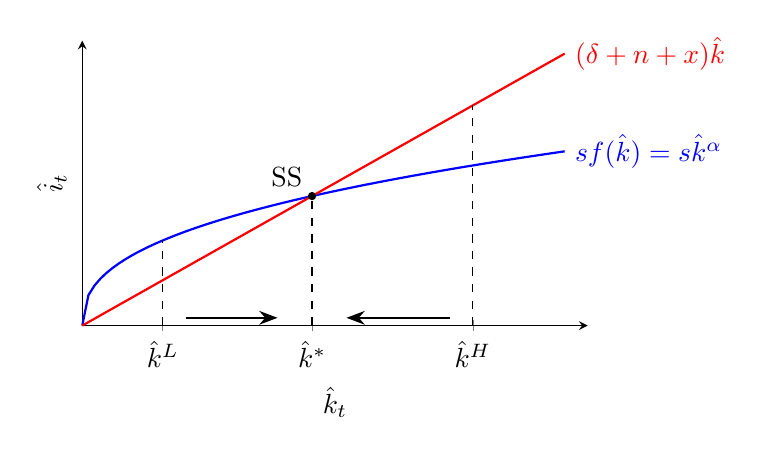
\begin{tikzpicture}
\begin{axis}[width=8cm,height=5.2cm,axis lines=left,xmin=0,xmax=2.2,ymin=0,ymax=1.1,
  xtick={0.35,1,1.7},xticklabels={$\hat k^L$,$\hat k^{*}$,$\hat k^H$},ytick=\empty,
  xlabel={$\hat k_t$},ylabel={$\hat i_t$},clip=false]
\addplot[thick,blue,domain=0:2.1,samples=80]{0.5*x^0.4} node[right]{$s f(\hat k)=s\hat k^{\alpha}$};
\addplot[thick,red,domain=0:2.1]{0.5*x} node[right]{$(\delta+n+x)\hat k$};
\fill (axis cs:1,0.5) circle(1.5pt) node[above left]{SS};
\draw[dashed] (axis cs:1,0)--(axis cs:1,0.5);
\draw[dashed] (axis cs:0.35,0)--(axis cs:0.35,0.33);
\draw[dashed] (axis cs:1.7,0)--(axis cs:1.7,0.85);
\draw[-{Stealth},thick] (axis cs:0.45,0.03)--(axis cs:0.85,0.03);
\draw[-{Stealth},thick] (axis cs:1.6,0.03)--(axis cs:1.15,0.03);
\end{axis}
\end{tikzpicture}
\end{center}
\textbf{How to read the diagram.} The horizontal axis is capital per effective worker $\hat k_t$; the vertical axis measures investment per effective worker. The blue curve is actual investment $s\hat k^{\alpha}$: it starts at the origin, is steep for small $\hat k$ and flattens out because of diminishing returns ($\alpha<1$). The red line is break-even investment $(\delta+n+x)\hat k$, a straight ray through the origin. By \eqref{eq:sol-fund}, $\dot{\hat k}$ is the vertical distance between the two; the arrows on the axis show the direction in which $\hat k$ moves.

\begin{itemize}
  \item $\hat k_t<\hat k^{*}$ (e.g.\ $\hat k^L$, low capital stock): $s\hat k_t^{\alpha}>(\delta+n+x)\hat k_t\Rightarrow\dot{\hat k}_t>0$, so $\hat k$ rises.
  \item $\hat k_t=\hat k^{*}$: $s\hat k_t^{\alpha}=(\delta+n+x)\hat k_t\Rightarrow\dot{\hat k}_t=0$, so $\hat k$ does not change over time.
  \item $\hat k_t>\hat k^{*}$ (e.g.\ $\hat k^H$, high capital stock): $s\hat k_t^{\alpha}<(\delta+n+x)\hat k_t\Rightarrow\dot{\hat k}_t<0$, so $\hat k$ falls.
\end{itemize}
\textbf{Why the crossing is unique and stable.} Divide \eqref{eq:sol-fund} by $\hat k$: $\dot{\hat k}/\hat k = s\hat k^{\alpha-1}-(\delta+n+x)$. The term $s\hat k^{\alpha-1}$ is strictly decreasing in $\hat k$ (since $\alpha-1<0$), tends to $+\infty$ as $\hat k\to0$ and to $0$ as $\hat k\to\infty$. So it crosses the constant $\delta+n+x$ exactly once, at $\hat k^*$; it is above it to the left and below it to the right.

\textit{Interpretation:} the system converges to the SS from any starting point $\hat k_0>0$. $\hat k$ grows only during the \emph{transition} (e.g.\ from $\hat k^L$ to $\hat k^{*}$); once the economy is at $\hat k^*$, growth of $\hat k$ stops.

%=====================================================================
\subsection{Technology development: a one-time rise in \texorpdfstring{$A$}{A} \pg{2}}

\paragraph{Experiment.} The economy is in SS. At date $t_0$ the technology level jumps once from $A$ to $A'>A$; afterwards it again grows at rate $x$. $K$ and $L$ cannot jump (they are stocks), and $s,n,\delta,x$ are unchanged.

\paragraph{Direct (impact) effect.} Per-capita output is $y=A^{1-\alpha}k^{\alpha}$ by (M1). Since $k=K/L$ is unchanged at $t_0$, $y$ jumps up immediately by the factor $(A'/A)^{1-\alpha}$: the production function itself has improved.

\paragraph{Indirect effect.} Capital per effective worker $\hat k=K/(AL)$ has $A$ in the denominator, so it falls at $t_0$ to $\hat k_{t_0}=K/(A'L)<\hat k^{*}$. In the phase diagram the curves do \emph{not} move: $\hat y=\hat k^{\alpha}$ and the break-even line do not depend on the level of $A$, so $\hat k^{*}$ in \eqref{eq:sol-kss} is unchanged. The economy simply jumps \emph{left} along the $\hat k$ axis. It is pushed back into the transition region: $\dot{\hat k}>0$, capital accumulation speeds up, and $\hat k$ converges back to the same $\hat k^{*}$.

\paragraph{Long run.} On the BGP $y_t=A_t(\hat k^*)^{\alpha}$, so the new long-run path of $y$ is higher than the old one by the full factor $A'/A$. The impact jump delivers $(A'/A)^{1-\alpha}$; the remaining factor $(A'/A)^{\alpha}$ comes from the extra capital accumulated during the transition.

\begin{center}
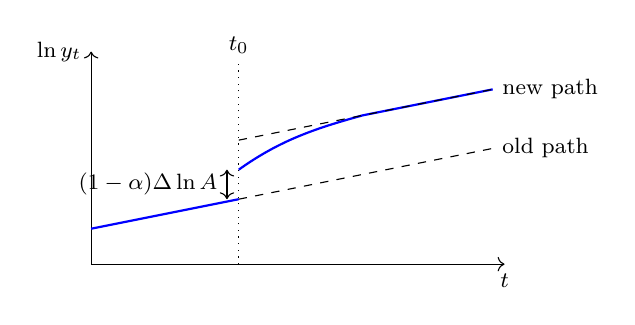
\begin{tikzpicture}[scale=0.75,every node/.style={font=\footnotesize}]
\draw[->](0,0)--(7,0) node[below]{$t$}; \draw[->](0,0)--(0,3.6) node[left]{$\ln y_t$};
\draw[dotted](2.5,0)--(2.5,3.4) node[above]{$t_0$};
\draw[thick,blue](0,0.6)--(2.5,1.1);
\draw[thick,blue](2.5,1.6) .. controls (3.2,2.1) and (3.8,2.3) .. (4.6,2.52)--(6.8,2.96);
\draw[dashed](2.5,1.1)--(6.8,1.96) node[right]{old path};
\draw[dashed](2.5,2.1)--(6.8,2.96);
\node[right] at (6.8,2.96){new path};
\draw[<->](2.3,1.1)--(2.3,1.6) node[midway,left]{$(1-\alpha)\Delta\ln A$};
\end{tikzpicture}
\end{center}
\textbf{How to read it.} The vertical axis is $\ln y$, so a constant growth rate shows up as a straight line with slope $x$. At $t_0$, $\ln y$ jumps by $(1-\alpha)\Delta\ln A$ (direct effect). It then grows faster than $x$ while $\hat k$ rebuilds (indirect effect), and finally runs along a new line of slope $x$ that lies $\Delta\ln A$ above the old one. The change in the level of $A$ has a level effect but no long-run growth effect.

%=====================================================================
\subsection{Evaluating the model against the growth facts \pg{3--5}}\label{sec:sol-eval}

Question: in the long run (and during transitions), do the variables of the Solow model behave like the variables in the data? Throughout we use \eqref{eq:sol-fund} and its growth-rate form
\begin{equation}\label{eq:sol-gk}
\frac{\dot{\hat k}_t}{\hat k_t}=s\hat k_t^{\alpha-1}-(\delta+n+x).
\end{equation}

\paragraph{Fact 1: in the long run, $y$ grows at the constant rate $x$.}
Step 1: relate growth of $y$ to growth of $\hat y$. Since $y_t=A_t\hat y_t$,
\begin{align*}
\frac{\dot y_t}{y_t} &= \frac{\dot A_t\hat y_t + A_t\dot{\hat y}_t}{A_t\hat y_t} && \text{(product rule)}\\
&= \frac{\dot A_t}{A_t} + \frac{\dot{\hat y}_t}{\hat y_t} = x + \frac{\dot{\hat y}_t}{\hat y_t}. \tag{F1a}
\end{align*}
Step 2: relate growth of $\hat y$ to growth of $\hat k$. Since $\hat y_t=\hat k_t^{\alpha}$,
\begin{align*}
\frac{\dot{\hat y}_t}{\hat y_t} &= \frac{\alpha\hat k_t^{\alpha-1}\dot{\hat k}_t}{\hat k_t^{\alpha}} && \text{(chain rule)}\\
&= \alpha\frac{\dot{\hat k}_t}{\hat k_t}. \tag{F1b}
\end{align*}
Because $\alpha$ is a constant, $\dot{\hat y}/\hat y$ depends only on $\dot{\hat k}/\hat k$.

Step 3: how does $\dot{\hat k}/\hat k$ change as the economy develops ($\hat k$ rises)? Differentiate \eqref{eq:sol-gk} with respect to $\hat k$:
\[
\frac{\partial(\dot{\hat k}/\hat k)}{\partial\hat k}=s(\alpha-1)\hat k^{\alpha-2}<0\qquad(\text{since }0<\alpha<1,\ s>0).
\]
Combined with (F1b), $\partial(\dot{\hat y}/\hat y)/\partial\hat k = \alpha s(\alpha-1)\hat k^{\alpha-2}<0$ as well.

Step 4: as $\hat k$ rises toward $\hat k^*$, the growth rates of $\hat k$ and $\hat y$ fall, reaching $0$ at the SS. Substituting into (F1a)--(F1b):
\[
\frac{\dot y_t}{y_t} = x+\alpha\frac{\dot{\hat k}_t}{\hat k_t}\ \longrightarrow\ x+\alpha\cdot 0 = x .
\]
\textit{Interpretation:} capital accumulation alone cannot sustain growth because of diminishing returns; in the long run per-capita income grows only because technology improves. The model reproduces fact 1, but the growth rate $x$ is exogenous (not explained).

\paragraph{Fact 2: balanced growth, $Y$, $C$, $I$ all grow at $x+n$.}
Write $Y_t=y_tL_t$ and take logs: $\ln Y_t=\ln y_t+\ln L_t$. Differentiate with respect to $t$:
\[
\frac{\dot Y_t}{Y_t}=\frac{\dot y_t}{y_t}+\frac{\dot L_t}{L_t}\ \longrightarrow\ x+n\quad\text{(long run, using fact 1)}.
\]
From (M2)--(M3), $C_t=(1-s)Y_t$ and $I_t=sY_t$. Taking logs, $\ln C_t=\ln(1-s)+\ln Y_t$; since $\ln(1-s)$ is a constant, its derivative is $0$, so $\dot C/C=\dot Y/Y=x+n$. In the same way $\dot I/I=\dot Y/Y=x+n$. The model displays balanced growth.

\paragraph{Fact 3: $K$ grows at a constant rate faster than $L$.}
Since $k_t=A_t\hat k_t$, by the product rule (as in (F1a))
\[
\frac{\dot k_t}{k_t}=\frac{\dot A_t}{A_t}+\frac{\dot{\hat k}_t}{\hat k_t} = x+\frac{\dot{\hat k}_t}{\hat k_t}\ \longrightarrow\ x \quad(\text{since } \dot{\hat k}/\hat k\to 0).
\]
Then $K_t=k_tL_t$ gives $\dot K/K=\dot k/k+n\to x+n$. This is constant, and it exceeds labour growth $n$ whenever $x>0$. So fact 3 holds as long as technology grows.

\paragraph{Fact 4: the rate of return to capital is constant.}
From (M5), $r_t=\text{MPK}=\alpha(A_tL_t)^{1-\alpha}K_t^{\alpha-1}=\alpha\hat k_t^{\alpha-1}$. The owner of capital earns $r_t$ but loses $\delta$ per unit through depreciation, so the net rate of return is
\[
r_t-\delta=\alpha\hat k_t^{\alpha-1}-\delta\ \longrightarrow\ \alpha(\hat k^*)^{\alpha-1}-\delta \quad\text{(long run)},
\]
a constant because $\hat k^*$ is constant. Similarly the labour share $w_tL_t/Y_t=1-\alpha$ is constant at all times.

\paragraph{Facts 6 and 7: conditional, not absolute, convergence.} The tools are:
(i) $y=A\hat y=A\hat k^{\alpha}$; (ii) $\dot y/y=x+\dot{\hat y}/\hat y$ (F1a); (iii) $\dot{\hat y}/\hat y=\alpha\,\dot{\hat k}/\hat k$ (F1b); (iv) $\dot{\hat k}/\hat k=s\hat k^{\alpha-1}-(\delta+n+x)$ \eqref{eq:sol-gk}; (v) $\partial(\dot{\hat k}/\hat k)/\partial\hat k<0$.
\begin{enumerate}[label=(\alph*)]
  \item \textbf{A country is poor because its $k=K/L$ is initially low, all parameters ($A$, $s$, $n$, $\delta$, $x$, $\alpha$) the same.}
  Low $k$ with the same $A$ means low $\hat k=k/A$, so by (i) $y$ is low. By (v), low $\hat k$ means a high $\dot{\hat k}/\hat k$, and by (ii)--(iii) a high $\dot y/y = x+\alpha\,\dot{\hat k}/\hat k$. The poor country is far below its SS, in its transition period, so it grows faster than the rich country. Both converge to the same $\hat k^*$ and the same path $y_t=A_t(\hat k^*)^{\alpha}$: \textbf{income convergence}.
  \item \textbf{A country is poor because its $A$ is low, all other parameters the same.}
  Both countries have the same $\hat k^*$ by \eqref{eq:sol-kss} (it does not depend on the level of $A$) and the same long-run growth rate $x$. In the long run $y^{P}_t/y^{R}_t = A^P_t(\hat k^*)^{\alpha}/(A^R_t(\hat k^*)^{\alpha}) = A^P/A^R<1$, a constant (both $A$'s grow at $x$). So the poor country \textbf{never catches up}: there is a permanent gap in income levels. During the transition, if the two countries start with similar $k$, the poor country has the \emph{higher} $\hat k=k/A$, hence by (v) the lower $\dot{\hat k}/\hat k$ and the lower $\dot y/y$: the relative gap widens (from $(A^P/A^R)^{1-\alpha}$ toward $A^P/A^R$) and then stays constant, while the absolute gap keeps growing at rate $x$.
  \item \textbf{Two countries have the same $y$ today, but one has a higher $s$ or a higher $x$.}
  Higher $s$ raises $\hat k^*$ \eqref{eq:sol-kss}, so the high-$s$ country is further below its SS and grows faster during the transition, toward a higher level path. Higher $x$ gives permanently faster long-run growth (fact 1). Either way the high-$s$/high-$x$ country grows faster: \textbf{divergence} from the same starting point.
\end{enumerate}
\textit{Conclusion:} the Solow model predicts convergence only among countries with similar parameters (conditional convergence, fact 7). Since not all countries are alike (poor countries may have lower $s$, $A$, or $x$), we should not expect a general narrowing of income gaps (no absolute convergence, fact 6).

\paragraph{Fact 5: large differences in income levels; growth miracles and disasters.}
On the BGP, combining $y_t=A_t\hat y^*$ with \eqref{eq:sol-kss},
\[
y_t = A_t\Big(\frac{s}{\delta+n+x}\Big)^{\frac{\alpha}{1-\alpha}} .
\]
Level differences can therefore come from differences in the technology level $A$ and, to some extent, the saving rate $s$. ``To some extent'': with $\alpha=1/3$ the exponent is $\alpha/(1-\alpha)=1/2$, so even a 4-fold difference in $s$ produces only a 2-fold difference in $y$. A 20-fold gap must therefore come mostly from $A$.

\emph{Speed of convergence.} How long can transitional growth last? Write \eqref{eq:sol-gk} in terms of $\ln\hat k$ and take a first-order Taylor expansion around $\ln\hat k^*$ (log-linearization: $f(u)\approx f(u^*)+f'(u^*)(u-u^*)$):
\begin{align*}
\frac{d\ln\hat k_t}{dt} &= s\,e^{-(1-\alpha)\ln\hat k_t}-(\delta+n+x) && \text{(since $\hat k^{\alpha-1}=e^{(\alpha-1)\ln\hat k}$)}\\
&\approx 0 - (1-\alpha)s(\hat k^*)^{\alpha-1}(\ln\hat k_t-\ln\hat k^*) && \text{(Taylor; value at SS is 0)}\\
&= -(1-\alpha)(\delta+n+x)(\ln\hat k_t-\ln\hat k^*) && \text{(SS: $s(\hat k^*)^{\alpha-1}=\delta+n+x$)}.
\end{align*}
So the log-gap to the SS closes at rate $\lambda=(1-\alpha)(\delta+n+x)$, the same $\lambda$ as in \eqref{eq:sol-path}. With $\alpha=1/3$ and $\delta+n+x=0.06$, $\lambda=0.04$: half of the gap closes in about $\ln 2/0.04\approx 17$ years. Transitional growth fades quickly as the SS is approached.

\begin{itemize}
  \item \textbf{Growth miracle} (5\% for decades): transitional growth cannot be sustained for long unless convergence is very slow, which requires a very high $\alpha$ (close to $1$, so $\lambda$ is small); otherwise it requires a high technology growth rate $x$.
  \item \textbf{Growth disaster:} requires a very low (or negative) value of $x$.
\end{itemize}

\begin{keybox}[title=Solow scorecard]
\begin{itemize}
  \item Long run: $\dot y/y=\dot k/k=x$; $\ \dot Y/Y=\dot C/C=\dot I/I=\dot K/K=x+n$; $\ r-\delta$ and factor shares constant. Facts 1--4 are reproduced.
  \item Predicts \emph{conditional} convergence (facts 6--7).
  \item Level differences come mainly from $A$ (and partly $s$); sustained growth comes only from the exogenous $x$, which the model does not explain.
\end{itemize}
\end{keybox}

%=====================================================================
\subsection{Welfare: the golden rule and dynamic (in)efficiency \pg{5--6}}

\paragraph{Setup.} Suppose a planner can choose the saving rate $s$ once and for all. Each $s$ gives a SS $\hat k^{ss}(s)$ via \eqref{eq:sol-kss}. Objective: find the $\hat k$ (and the $s$ that delivers it) that maximizes steady-state consumption per effective worker $\hat c^{ss}$. This is the \textbf{golden rule}.

\paragraph{Steady-state consumption as a function of $\hat k$.} In SS actual investment equals break-even investment, $\hat i^{ss}=s\hat y^{ss}=(\delta+n+x)\hat k^{ss}$, and $\hat y^{ss}=(\hat k^{ss})^{\alpha}$. Using (M2):
\begin{align*}
\hat c^{ss} &= \hat y^{ss}-\hat i^{ss} && \text{(M2)}\\
&= (\hat k^{ss})^{\alpha}-(\delta+n+x)\hat k^{ss}. && \text{(substitute SS values)}
\end{align*}

\paragraph{Maximizing.} Treat $\hat k$ as the choice variable:
\begin{align*}
\frac{\partial\hat c^{ss}}{\partial\hat k} &= \alpha\hat k^{\alpha-1}-(\delta+n+x)=0 && \text{(FOC)}\\
\alpha\hat k^{\alpha-1} &= \delta+n+x && \text{(i.e.\ $r=\delta+n+x$ by (M5))}\\
\hat k^{1-\alpha} &= \frac{\alpha}{\delta+n+x} && \text{(invert: $\hat k^{\alpha-1}=1/\hat k^{1-\alpha}$)}\\
\hat k_{gold} &= \Big(\frac{\alpha}{\delta+n+x}\Big)^{\frac{1}{1-\alpha}} .
\end{align*}
Second-order condition: $\partial^2\hat c^{ss}/\partial\hat k^2=\alpha(\alpha-1)\hat k^{\alpha-2}<0$, so this is a maximum. Since $\hat c^{ss}(\hat k)$ is concave, it is increasing for $\hat k<\hat k_{gold}$ and decreasing for $\hat k>\hat k_{gold}$.

\paragraph{Which saving rate delivers the golden rule?} Compare the two expressions
\[
\hat k^{ss}=\Big(\frac{s}{\delta+n+x}\Big)^{\frac1{1-\alpha}},\qquad
\hat k_{gold}=\Big(\frac{\alpha}{\delta+n+x}\Big)^{\frac1{1-\alpha}} .
\]
They are equal exactly when $s=\alpha$. Because $\hat k^{ss}$ is strictly increasing in $s$, $s>\alpha\Leftrightarrow\hat k^{ss}>\hat k_{gold}$ and $s<\alpha\Leftrightarrow\hat k^{ss}<\hat k_{gold}$.

\begin{center}
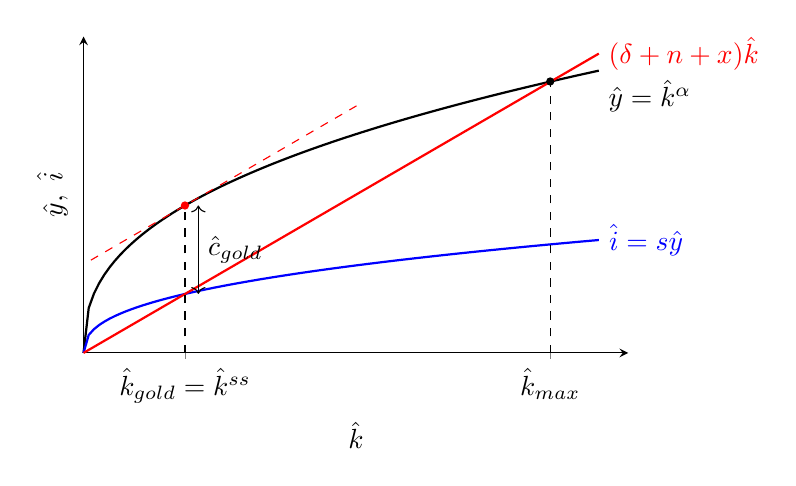
\begin{tikzpicture}
\begin{axis}[width=8.5cm,height=5.6cm,axis lines=left,xmin=0,xmax=3.7,ymin=0,ymax=1.85,
  xtick={0.689,3.17},xticklabels={$\hat k_{gold}=\hat k^{ss}$,$\hat k_{max}$},ytick=\empty,
  xlabel={$\hat k$},ylabel={$\hat y,\ \hat i$},clip=false]
\addplot[thick,black,domain=0:3.5,samples=100]{x^0.4};
\node[right] at (axis cs:3.5,1.5){$\hat y=\hat k^{\alpha}$};
\addplot[thick,blue,domain=0:3.5,samples=100]{0.4*x^0.4} node[right]{$\hat i=s\hat y$};
\addplot[thick,red,domain=0:3.5]{0.5*x};
\node[red,right] at (axis cs:3.5,1.75){$(\delta+n+x)\hat k$};
\addplot[dashed,red,domain=0.05:1.9]{0.862+0.5*(x-0.689)};
\fill[red] (axis cs:0.689,0.862) circle(1.5pt);
\fill (axis cs:3.17,1.587) circle(1.5pt);
\draw[dashed] (axis cs:0.689,0)--(axis cs:0.689,0.862);
\draw[dashed] (axis cs:3.17,0)--(axis cs:3.17,1.587);
\draw[<->] (axis cs:0.78,0.345)--(axis cs:0.78,0.862) node[midway,right]{$\hat c_{gold}$};
\end{axis}
\end{tikzpicture}
\end{center}
\textbf{How to read the diagram.} The black curve is output $\hat y$, the blue curve is investment $s\hat y$ and the red line is break-even investment. In SS, consumption $\hat c^{ss}$ is the vertical gap between $\hat y$ and the red line (because $\hat i^{ss}$ equals break-even investment). This gap is largest where the slope of $\hat y$ equals the slope of the red line, $\delta+n+x$: the dashed tangent touches $\hat y$ at $\hat k_{gold}$ and is parallel to the red line. The figure is drawn with $s=\alpha$, so the blue curve crosses the red line exactly at $\hat k_{gold}$. At $\hat k_{max}$ (where $\hat y$ meets the red line) all output must be invested to keep $\hat k$ constant ($s=1$) and consumption is zero.

\begin{keybox}[title=Golden rule and dynamic efficiency]
\[
\alpha\hat k_{gold}^{\alpha-1}=\delta+n+x\ \ (\text{i.e. } r-\delta=n+x),\qquad
\hat k_{gold}=\Big(\frac{\alpha}{\delta+n+x}\Big)^{\frac1{1-\alpha}},\qquad s_{gold}=\alpha .
\]
\begin{itemize}
  \item \textbf{Case 1, $s>\alpha$:} $\hat k^{ss}>\hat k_{gold}$. The economy is \textbf{dynamically inefficient}: lowering $s$ makes agents better off in \emph{all} periods.
  \item \textbf{Case 2, $0\le s<\alpha$:} $\hat k^{ss}<\hat k_{gold}$. The economy is \textbf{dynamically efficient}: changing $s$ involves a trade-off between periods, so no change is a Pareto improvement.
\end{itemize}
\end{keybox}
\textit{Interpretation of the golden rule condition:} at the golden rule the net return on capital $r-\delta$ equals the growth rate of the economy $n+x$. If $r-\delta<n+x$, there is ``too much'' capital: the extra output from the marginal unit of capital is less than what is needed just to maintain it.

\paragraph{Case 1 ($s>\alpha$): what happens if we lower $s$ to $\alpha$ at date $t_0$?}
\begin{enumerate}
  \item \textbf{$\hat k$ and $\hat y$.} Before $t_0$, $\dot{\hat k}=s\hat y-(\delta+n+x)\hat k=0$ at the old SS. At $t_0$, $s$ falls while $\hat k$ (a stock) cannot jump, so $s\hat y$ falls and $\dot{\hat k}<0$. $\hat k$ declines smoothly until it reaches the new SS, $\hat k_{gold}$. Since $\hat y_t=\hat k_t^{\alpha}$, $\hat y$ has the same shape.
  \item \textbf{$\hat c=(1-s)\hat y$.} At $t_0$, $\hat y$ is unchanged but $1-s$ rises, so $\hat c$ \emph{jumps up}. Afterwards $\hat c_t=(1-\alpha)\hat y_t$ falls with $\hat y$, settling at $\hat c_{gold}$. Since $\hat c^{ss}(\hat k)$ is maximized at $\hat k_{gold}$, $\hat c_{gold}>\hat c_{old}$. And since $\hat c_t$ declines monotonically toward $\hat c_{gold}$, it stays above $\hat c_{old}$ at every date. Consumption is higher in all periods: this is why $s>\alpha$ is inefficient.
  \item \textbf{$\hat i=s\hat y$.} At $t_0$, $\hat i$ jumps down (lower $s$, same $\hat y$), then declines further with $\hat y$ and levels off at the new SS.
\end{enumerate}
\begin{center}
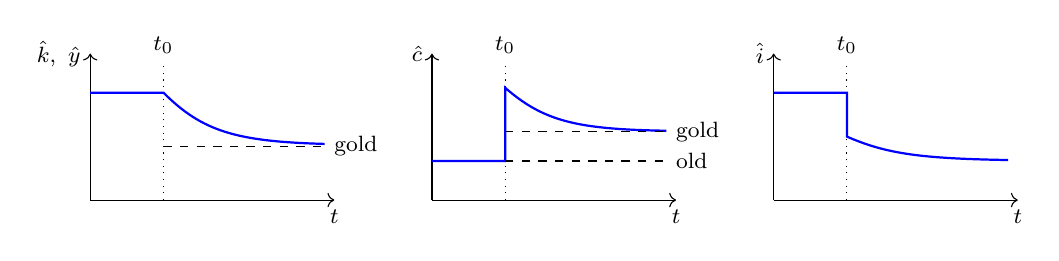
\begin{tikzpicture}[scale=0.62,every node/.style={font=\footnotesize}]
\draw[->](0,0)--(5,0) node[below]{$t$}; \draw[->](0,0)--(0,3) node[left]{$\hat k,\ \hat y$};
\draw[dotted](1.5,0)--(1.5,2.8) node[above]{$t_0$};
\draw[thick,blue](0,2.2)--(1.5,2.2) .. controls (2.3,1.4) and (3,1.2) .. (4.8,1.15);
\draw[dashed](1.5,1.1)--(4.8,1.1) node[right]{gold};
\begin{scope}[shift={(7,0)}]
\draw[->](0,0)--(5,0) node[below]{$t$}; \draw[->](0,0)--(0,3) node[left]{$\hat c$};
\draw[dotted](1.5,0)--(1.5,2.8) node[above]{$t_0$};
\draw[thick,blue](0,0.8)--(1.5,0.8)--(1.5,2.3) .. controls (2.3,1.6) and (3,1.45) .. (4.8,1.42);
\draw[dashed](1.5,0.8)--(4.8,0.8) node[right]{old};
\draw[dashed](1.5,1.4)--(4.8,1.4) node[right]{gold};
\end{scope}
\begin{scope}[shift={(14,0)}]
\draw[->](0,0)--(5,0) node[below]{$t$}; \draw[->](0,0)--(0,3) node[left]{$\hat i$};
\draw[dotted](1.5,0)--(1.5,2.8) node[above]{$t_0$};
\draw[thick,blue](0,2.2)--(1.5,2.2)--(1.5,1.3) .. controls (2.3,0.95) and (3,0.85) .. (4.8,0.82);
\end{scope}
\end{tikzpicture}
\end{center}
\textbf{How to read the panels.} Each panel plots one variable against time, with the policy change at $t_0$ (dotted line). Stocks ($\hat k$, and hence $\hat y$) move continuously; flows that depend directly on $s$ ($\hat c$, $\hat i$) jump at $t_0$ and then follow $\hat y$. In the middle panel the whole post-$t_0$ path of $\hat c$ lies above the old level.

\paragraph{Case 2 ($s<\alpha$): dynamic efficiency.} Here a change in $s$ creates a trade-off: it raises consumption and welfare in some periods but lowers it in others. For example, raising $s$ increases future $\hat k$ and output but reduces current $\hat c$ (see the next subsection); lowering $s$ raises $\hat c$ today but lowers it in the long run. No change in $s$ makes every period better off, so the allocation cannot be improved for all generations.

%=====================================================================
\subsection{Effects of a rise in \texorpdfstring{$s$}{s} (dynamically efficient region) \pg{8}}

\paragraph{Experiment.} The economy is in SS with $s_{old}<\alpha$. At $t_0$ the saving rate rises permanently to $s_{new}$ with $s_{old}<s_{new}\le\alpha$. All other parameters are unchanged; $\hat k$ cannot jump at $t_0$.

\begin{enumerate}
  \item \textbf{Growth rate of $\hat k$.} By \eqref{eq:sol-gk}, $\dot{\hat k}/\hat k=s\hat k^{\alpha-1}-(\delta+n+x)$. Before $t_0$ it equals $0$. At $t_0$, $s$ jumps up with $\hat k$ fixed, so $\dot{\hat k}/\hat k$ jumps up to a positive value. As $\hat k$ then rises, $s_{new}\hat k^{\alpha-1}$ falls, so $\dot{\hat k}/\hat k$ decays back to $0$.
  \item \textbf{Level of $\hat k$.} $\hat k$ rises, at a slowing pace, to a higher plateau. The new SS solves $s_{new}\hat k^{\alpha}=(\delta+n+x)\hat k$, so by \eqref{eq:sol-kss} $\hat k^{ss}_{new}=(s_{new}/(\delta+n+x))^{1/(1-\alpha)}>\hat k^{ss}_{old}$: the investment curve $s\hat k^\alpha$ shifts up and crosses the break-even line further right.
  \item \textbf{Growth rate of income per capita $y=Y/L$.} By (F1a)--(F1b), $\dot y/y=x+\alpha\,\dot{\hat k}/\hat k$. So $\dot y/y$ has the same shape as in item 1, scaled by $\alpha$, but it starts from and returns to $x$ (not $0$).
  \item \textbf{$\ln y$.} The slope of $\ln y$ against $t$ is $\dot y/y$. Before $t_0$ it is a straight line of slope $x$. After $t_0$ it becomes steeper, then bends back to slope $x$. It ends on a line parallel to, and above, the old path. The rise in $s$ has a \emph{level} effect, not a long-run \emph{growth} effect.
  \item \textbf{$\hat c=(1-s)\hat y$.} At $t_0$, $\hat y$ is fixed but $1-s$ falls, so $\hat c$ drops. Then, as $\hat k$ and $\hat y$ rise, $\hat c$ recovers and settles at a new SS above the old one: since $\hat k^{ss}_{old}<\hat k^{ss}_{new}\le\hat k_{gold}$ and $\hat c^{ss}(\hat k)$ is increasing below $\hat k_{gold}$. If $s_{new}=\alpha$, the new SS level is $\hat c_{gold}$. Current generations lose and future ones gain: the trade-off of dynamic efficiency.
\end{enumerate}

\begin{center}
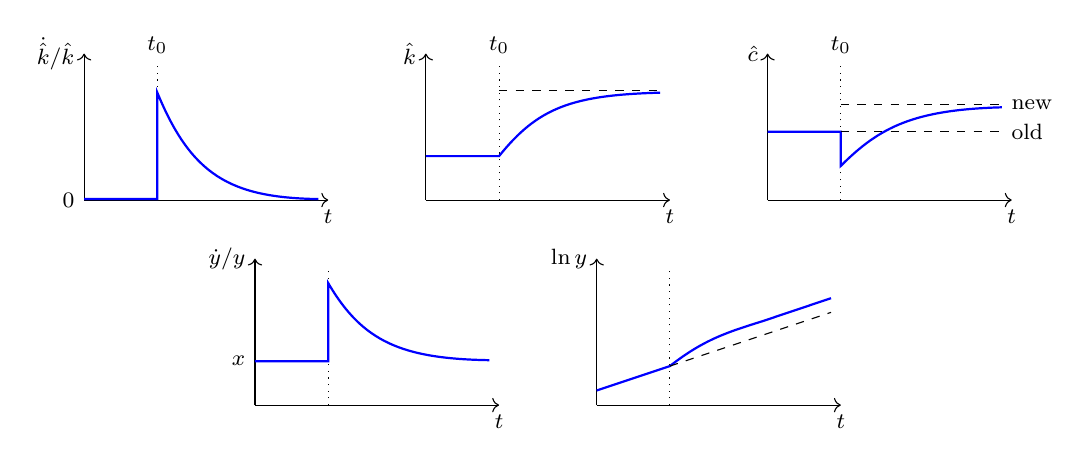
\begin{tikzpicture}[scale=0.62,every node/.style={font=\footnotesize}]
% row 1
\draw[->](0,0)--(5,0) node[below]{$t$}; \draw[->](0,0)--(0,3) node[left]{$\dot{\hat k}/\hat k$};
\draw[dotted](1.5,0)--(1.5,2.8) node[above]{$t_0$}; \node[left] at (0,0){$0$};
\draw[thick,blue](0,0.02)--(1.5,0.02)--(1.5,2.2) .. controls (2.2,0.5) and (3,0.05) .. (4.8,0.02);
\begin{scope}[shift={(7,0)}]
\draw[->](0,0)--(5,0) node[below]{$t$}; \draw[->](0,0)--(0,3) node[left]{$\hat k$};
\draw[dotted](1.5,0)--(1.5,2.8) node[above]{$t_0$};
\draw[thick,blue](0,0.9)--(1.5,0.9) .. controls (2.3,1.9) and (3,2.15) .. (4.8,2.2);
\draw[dashed](1.5,2.25)--(4.8,2.25);
\end{scope}
\begin{scope}[shift={(14,0)}]
\draw[->](0,0)--(5,0) node[below]{$t$}; \draw[->](0,0)--(0,3) node[left]{$\hat c$};
\draw[dotted](1.5,0)--(1.5,2.8) node[above]{$t_0$};
\draw[thick,blue](0,1.4)--(1.5,1.4)--(1.5,0.7) .. controls (2.3,1.5) and (3,1.85) .. (4.8,1.9);
\draw[dashed](1.5,1.4)--(4.8,1.4) node[right]{old};
\draw[dashed](1.5,1.95)--(4.8,1.95) node[right]{new};
\end{scope}
% row 2
\begin{scope}[shift={(3.5,-4.2)}]
\draw[->](0,0)--(5,0) node[below]{$t$}; \draw[->](0,0)--(0,3) node[left]{$\dot y/y$};
\draw[dotted](1.5,0)--(1.5,2.8); \node[left] at (0,0.9){$x$};
\draw[thick,blue](0,0.9)--(1.5,0.9)--(1.5,2.5) .. controls (2.2,1.3) and (3,0.95) .. (4.8,0.92);
\end{scope}
\begin{scope}[shift={(10.5,-4.2)}]
\draw[->](0,0)--(5,0) node[below]{$t$}; \draw[->](0,0)--(0,3) node[left]{$\ln y$};
\draw[dotted](1.5,0)--(1.5,2.8);
\draw[thick,blue](0,0.3)--(1.5,0.8) .. controls (2.2,1.35) and (2.7,1.5) .. (3.4,1.72)--(4.8,2.19);
\draw[dashed](1.5,0.8)--(4.8,1.9);
\end{scope}
\end{tikzpicture}
\end{center}
\textbf{How to read the panels.} Top row: growth of $\hat k$ (jumps, then decays to $0$), the level of $\hat k$ (rises smoothly to the higher SS), and consumption $\hat c$ (drops at $t_0$, then overshoots the old level). Bottom row: $\dot y/y$ (jumps above $x$, then returns to $x$) and $\ln y$, whose slope is $\dot y/y$. The dashed line in the $\ln y$ panel is the old path: the new path is steeper for a while and then runs parallel to it at a higher level.

\begin{tipbox}
In the Solow model a change in $s$ (or in the level of $A$) never changes the long-run growth rate of $y$; only $x$ does. Always draw $\ln y$ returning to slope $x$, parallel to the old path.
\end{tipbox}

%=====================================================================
\subsection{Application: foreign aid \pg{7}}

\paragraph{Setup.} A poor country is described by \eqref{eq:sol-fund}. Let ``aid'' denote the amount of aid per effective worker, received each period (a constant). Compare four forms of aid.

\begin{enumerate}
  \item \textbf{Consumption goods.} The aid is consumed directly:
  \[
  \hat c_t=(1-s)\hat k_t^{\alpha}+\text{aid},\qquad \dot{\hat k}_t=s\hat k_t^{\alpha}-(\delta+n+x)\hat k_t\ \ \text{(unchanged)}.
  \]
  The accumulation equation is unaffected, so the aid has no effect on the factors of production ($\hat k$, $\hat k^*$ and $\hat y$ are unchanged). It provides only temporary relief: more aid will be required in the future. It may still be necessary (e.g.\ famine relief) even though it is not a lasting solution.
  \item \textbf{Capital goods (a one-time transfer of capital).} Poor countries have low $\hat k$, so they are far below their SS. A transfer of capital raises $\hat k$ immediately, moving the economy to the right along the $\hat k$ axis in the phase diagram, and so speeds up the development process. The gain is lasting in the sense that it does not need to be repeated: the country is permanently further along its transition. But $\hat k^*$ in \eqref{eq:sol-kss} is unchanged, so the long-run path of $y$ is the same.
  \item \textbf{Technical assistance ($A\uparrow$).} Poor countries also have low technology levels. As in the one-time rise in $A$ above: the \emph{direct} effect raises $y$ immediately; the \emph{indirect} effect lowers $\hat k=K/(AL)$, pushing the economy back into transitional growth, so capital accumulation starts again. Long-run $y$ is permanently higher.
  \item \textbf{Money.} Money is not capital: the country treats the aid as extra income, saves only the fraction $s$ of it and consumes the rest. Investment per effective worker becomes $\hat i_t=s(\hat k_t^{\alpha}+\text{aid})$, so
  \begin{equation}\label{eq:sol-aid}
  \dot{\hat k}_t=s\hat k_t^{\alpha}+s\cdot\text{aid}-(\delta+n+x)\hat k_t .
  \end{equation}
\end{enumerate}

\paragraph{Effect of money aid on the steady state.} The new SS $\hat k^{ss}_{new}$ solves $s(\hat k^{\alpha}+\text{aid})=(\delta+n+x)\hat k$.
\begin{itemize}
  \item At the old SS $\hat k^{ss}$, $s(\hat k^{ss})^{\alpha}=(\delta+n+x)\hat k^{ss}$, so \eqref{eq:sol-aid} gives $\dot{\hat k}=s\cdot\text{aid}>0$: $\hat k$ starts to rise, and $\hat k^{ss}_{new}>\hat k^{ss}$.
  \item Implicit function theorem (if $F(\hat k,a)=0$ then $d\hat k/da=-F_a/F_{\hat k}$) with $F=s\hat k^{\alpha}+s\,a-(\delta+n+x)\hat k$ and $a=\text{aid}$:
  \[
  \frac{d\hat k^{ss}_{new}}{d\,\text{aid}}=\frac{s}{(\delta+n+x)-s\alpha\hat k^{\alpha-1}} .
  \]
  The denominator is positive: at the new SS, $(\delta+n+x)\hat k=s\hat k^{\alpha}+s\cdot\text{aid}>s\hat k^{\alpha}$, so $\delta+n+x>s\hat k^{\alpha-1}>s\alpha\hat k^{\alpha-1}$. Hence the effect is positive, and it is proportional to $s$.
\end{itemize}
\textit{Interpretation:} the effectiveness of money aid in raising $\hat k$ depends in part on $s$. If the fraction of the aid money that is saved is low, it does little for capital accumulation; most of it simply raises consumption, as in case 1.

\begin{center}
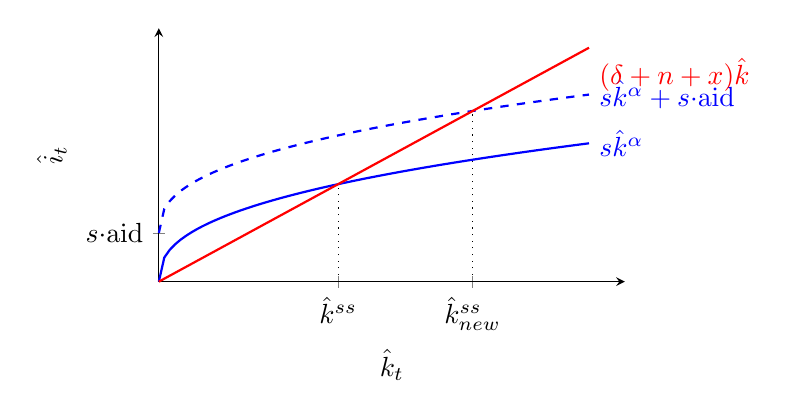
\begin{tikzpicture}
\begin{axis}[width=7.5cm,height=4.8cm,axis lines=left,xmin=0,xmax=2.6,ymin=0,ymax=1.3,
  xtick={1,1.75},xticklabels={$\hat k^{ss}$,$\hat k^{ss}_{new}$},ytick={0.25},yticklabels={$s\cdot$aid},
  xlabel={$\hat k_t$},ylabel={$\hat i_t$},clip=false]
\addplot[thick,blue,domain=0:2.4,samples=80]{0.5*x^0.4} node[right]{$s\hat k^{\alpha}$};
\addplot[thick,blue,dashed,domain=0:2.4,samples=80]{0.25+0.5*x^0.4} node[right]{$s\hat k^{\alpha}+s\cdot$aid};
\addplot[thick,red,domain=0:2.4]{0.5*x} node[below right]{$(\delta+n+x)\hat k$};
\draw[dotted](axis cs:1,0)--(axis cs:1,0.5); \draw[dotted](axis cs:1.75,0)--(axis cs:1.75,0.875);
\end{axis}
\end{tikzpicture}
\end{center}
\textbf{How to read the diagram.} Money aid shifts the investment curve up by the constant $s\cdot\text{aid}$, so the dashed curve starts at the intercept $s\cdot\text{aid}$ on the vertical axis. It crosses the unchanged break-even line further to the right, at $\hat k^{ss}_{new}$. The smaller $s$ is, the smaller the upward shift and the smaller the gain in $\hat k^{ss}$.

%=====================================================================
\subsection{Solow model with land and natural resources \pg{9--10}}

\paragraph{Question.} How would a fixed factor (land) and a non-renewable resource affect the long-run growth rate of an economy?

\paragraph{Setup.}
\begin{itemize}
  \item Inputs: capital $K_t$, effective labour $A_tL_t$, a non-renewable natural resource $R_t$ (the amount used in production each period), and land $T_t$.
  \item Growth assumptions: $\dot L_t/L_t=n$, $\dot A_t/A_t=x$, $\dot R_t/R_t=-b$ with $b>0$ (the resource input shrinks at rate $b$ as it is depleted), $\dot T_t=0$ (land is fixed).
  \item Exponents $\alpha,\beta,\gamma>0$ with $\alpha+\beta+\gamma<1$; effective labour gets exponent $1-\alpha-\beta-\gamma>0$, so production has constant returns in all four inputs.
  \item Saving rule and depreciation as before: $I_t=sY_t$, depreciation rate $\delta$.
\end{itemize}
\begin{align}
Y_t&=(A_tL_t)^{1-\alpha-\beta-\gamma}K_t^{\alpha}R_t^{\beta}T_t^{\gamma}, \label{eq:sol-lr1}\\
\dot K_t&=I_t-\delta K_t=sY_t-\delta K_t\ \Longrightarrow\ \frac{\dot K_t}{K_t}=s\frac{Y_t}{K_t}-\delta \quad\text{(divide by $K_t$)}. \label{eq:sol-lr2}
\end{align}

\paragraph{Growth rate of output.} Take logs of \eqref{eq:sol-lr1}:
\[
\ln Y_t=(1-\alpha-\beta-\gamma)(\ln A_t+\ln L_t)+\alpha\ln K_t+\beta\ln R_t+\gamma\ln T_t .
\]
Differentiate with respect to $t$, using $d\ln X/dt=\dot X/X$:
\begin{align*}
\frac{\dot Y_t}{Y_t}&=(1-\alpha-\beta-\gamma)\Big(\frac{\dot A_t}{A_t}+\frac{\dot L_t}{L_t}\Big)+\alpha\frac{\dot K_t}{K_t}+\beta\frac{\dot R_t}{R_t}+\gamma\frac{\dot T_t}{T_t}\\
&=(1-\alpha-\beta-\gamma)(x+n)+\alpha\frac{\dot K_t}{K_t}+\beta(-b)+\gamma\cdot 0 .
\end{align*}
\begin{equation}\label{eq:sol-lr3}
\frac{\dot Y_t}{Y_t}=(1-\alpha-\beta-\gamma)(x+n)-\beta b+\alpha\frac{\dot K_t}{K_t}.
\end{equation}

\paragraph{Balanced growth path (BGP).} Suppose a BGP exists on which $Y$ and $K$ grow at the same constant rate $g$. (This is the only possibility with constant growth: by \eqref{eq:sol-lr2}, constant $\dot K/K$ requires constant $Y/K$, i.e.\ $\dot Y/Y=\dot K/K$.) Set $\dot Y/Y=\dot K/K=g$ in \eqref{eq:sol-lr3}:
\begin{align*}
g&=(1-\alpha-\beta-\gamma)(x+n)-\beta b+\alpha g\\
(1-\alpha)g&=(1-\alpha-\beta-\gamma)(x+n)-\beta b && \text{(move $\alpha g$ to the left)}
\end{align*}
\begin{equation}\label{eq:sol-lr4}
g=\Big[\frac{1-\alpha-\beta-\gamma}{1-\alpha}\Big](x+n)-\Big[\frac{\beta}{1-\alpha}\Big]b \qquad\text{(divide by $1-\alpha>0$)}.
\end{equation}

\paragraph{Does the economy converge to the BGP?} Yes. Subtract \eqref{eq:sol-lr4}, written as $g=(1-\alpha-\beta-\gamma)(x+n)-\beta b+\alpha g$, from \eqref{eq:sol-lr3}; the constant terms cancel:
\begin{equation}\label{eq:sol-lr5}
\frac{\dot Y_t}{Y_t}-g=\alpha\Big(\frac{\dot K_t}{K_t}-g\Big).
\end{equation}
Recall from \eqref{eq:sol-lr2} that $\dot K/K$ moves in the same direction as $Y/K$, and $Y/K$ rises when $\dot Y/Y>\dot K/K$ and falls when $\dot Y/Y<\dot K/K$.
\begin{itemize}
  \item[(i)] $\dot K/K>g$. By \eqref{eq:sol-lr5} the RHS is positive, so $\dot Y/Y>g$. But since $\alpha<1$, $\dot Y/Y-g<\dot K/K-g$, i.e.\ $\dot Y/Y<\dot K/K$. So $Y/K$ falls during the transition, and by \eqref{eq:sol-lr2} $\dot K/K$ falls toward $g$.
  \item[(ii)] $\dot K/K<g$. By \eqref{eq:sol-lr5}, $\dot Y/Y<g$, and since $\alpha<1$, $\dot Y/Y>\dot K/K$. So $Y/K$ rises, and by \eqref{eq:sol-lr2} $\dot K/K$ rises toward $g$.
  \item[(iii)] $\dot K/K=g$. By \eqref{eq:sol-lr5}, $\dot Y/Y=g$, so $Y/K$ is constant and $\dot K/K$ stays at $g$.
\end{itemize}
\textit{Conclusion:} from (i)--(iii), the economy moves toward the BGP regardless of initial conditions, and once it reaches the BGP it remains there.

\paragraph{Long-run growth of per-capita variables.} All per-capita variables (e.g.\ $y=Y/L$, $k=K/L$) grow at $g-n$. Subtract $n$ from \eqref{eq:sol-lr4}:
\begin{align*}
g-n&=\frac{(1-\alpha-\beta-\gamma)(x+n)-\beta b-(1-\alpha)n}{1-\alpha} && \text{(common denominator)}\\
&=\frac{(1-\alpha-\beta-\gamma)x+\big[(1-\alpha-\beta-\gamma)-(1-\alpha)\big]n-\beta b}{1-\alpha} && \text{(collect $n$)}\\
&=\frac{(1-\alpha-\beta-\gamma)x-(\beta+\gamma)n-\beta b}{1-\alpha} .
\end{align*}
\begin{keybox}[title=Long-run per-capita growth with land and resources]
\begin{equation}\label{eq:sol-lr6}
g-n=\underbrace{\Big[\frac{1-\alpha-\beta-\gamma}{1-\alpha}\Big]x}_{(a)}-\underbrace{\Big[\frac{\beta}{1-\alpha}\Big]b}_{(b)}-\underbrace{\Big[\frac{\beta+\gamma}{1-\alpha}\Big]n}_{(c)}
\end{equation}
\begin{itemize}
  \item (b) \textbf{Resource depletion:} the resource is being used up, so less is available each period. This adversely affects production, and growth slows.
  \item (c) \textbf{Congestion:} with a depletable resource and a fixed factor, population growth means each worker has less land and less resource to work with. This congestion slows per-capita growth.
  \item (a) \textbf{Technology:} $g-n$ can still be positive if $x$ is sufficiently large, precisely if $(1-\alpha-\beta-\gamma)x>\beta b+(\beta+\gamma)n$. Technological progress can outrun depletion and congestion.
\end{itemize}
\end{keybox}
\textit{Check:} with no land and no resource ($\beta=\gamma=0$), \eqref{eq:sol-lr6} reduces to $g-n=x$, the standard Solow result (fact 1).

\section{The Ramsey(-Cass-Koopmans) Model and Fiscal Policy / Endogenous Growth}

The Solow model takes the saving rate as a fixed parameter. The Ramsey(-Cass-Koopmans) model keeps the same production side but lets households \emph{choose} how much to consume and save by maximising lifetime utility. The saving rate therefore becomes an outcome that depends on preferences. We then use the model to study fiscal policy (lump-sum and proportional taxes), and finally productive government spending, which can generate endogenous (policy-dependent) long-run growth.

%==============================================================
\subsection{Setup \pg{27}}

\paragraph{Timing and notation.} Time $t\ge0$ is \emph{continuous}. A dot denotes a time derivative, $\dot z_t\equiv dz_t/dt$, and $\dot z_t/z_t$ is the growth rate of $z_t$. A hat denotes a quantity \emph{per effective worker}, i.e.\ divided by $A_tL_t$.

\begin{itemize}
\item $Y_t$, $K_t$, $C_t$, $I_t$: aggregate output, capital stock, consumption, gross investment.
\item $L_t=L_0e^{nt}$: population = labour force; $n$ = population growth rate. Normalise $L_0=1$.
\item $A_t=A_0e^{xt}$: labour-augmenting technology, so $\dot A_t/A_t=x$; $x$ = rate of technological progress. Normalise $A_0=1$ where convenient.
\item $\hat k_t=K_t/(A_tL_t)$, $\hat y_t=Y_t/(A_tL_t)$, $\hat c_t=C_t/(A_tL_t)$, $\hat i_t=I_t/(A_tL_t)$: capital, output, consumption, investment per effective worker.
\item $w_t$: real wage per worker; $r_t$: rental rate of capital (gross of depreciation); $\delta$: depreciation rate.
\item $\alpha\in(0,1)$: capital share in production.
\item $\rho>0$: rate of time preference (subjective discount rate).
\item $\theta>0$: curvature of utility; $1/\theta$ is the intertemporal elasticity of substitution (IES).
\end{itemize}

\paragraph{Firms.} Many competitive firms rent capital and hire labour. They take the prices $w_t$ and $r_t$ as given and choose the \emph{inputs} $K_t$ and $L_t$:
\[
\max_{K_t,\,L_t}\ \pi_t = Y_t - w_tL_t - r_tK_t,\qquad Y_t=(A_tL_t)^{1-\alpha}K_t^{\alpha}.
\]
Dividing the production function by $A_tL_t$ gives the intensive form
\[
\hat y_t=\frac{(A_tL_t)^{1-\alpha}K_t^\alpha}{A_tL_t}=\Big(\frac{K_t}{A_tL_t}\Big)^{\alpha}=\hat k_t^{\alpha}.
\]
The first-order conditions set each price equal to the marginal product:
\begin{align}
r_t&=\frac{\partial Y_t}{\partial K_t}=\alpha (A_tL_t)^{1-\alpha}K_t^{\alpha-1}=\alpha\hat k_t^{\alpha-1}\qquad(=MPK), \label{rm:r}\\
w_t&=\frac{\partial Y_t}{\partial L_t}=(1-\alpha)A_t^{1-\alpha}L_t^{-\alpha}K_t^{\alpha}=(1-\alpha)A_t\hat k_t^{\alpha}. \label{rm:w}
\end{align}
A useful identity follows (Euler's theorem for constant returns to scale, i.e.\ factor payments exhaust output):
\begin{equation}
\frac{w_t}{A_t}+r_t\hat k_t=(1-\alpha)\hat k_t^\alpha+\alpha\hat k_t^{\alpha-1}\hat k_t=\hat k_t^\alpha=\hat y_t. \label{rm:exhaust}
\end{equation}

\paragraph{Households.} The economy has a large number of identical, infinitely lived households, so we can study one representative household. It owns the capital, rents it to firms, supplies labour inelastically, and takes $w_t,r_t$ as given. Period utility is CRRA:
\[
u(c)=\frac{c^{1-\theta}}{1-\theta},\qquad u'(c)=c^{-\theta}>0,\qquad u''(c)=-\theta c^{-\theta-1}<0 .
\]

\emph{From per-capita to per-effective-worker utility.} The household weights each member's utility, $L_t\,u(c_t)$ with $c_t=C_t/L_t=A_t\hat c_t$ consumption per person, and discounts at $\rho$:
\begin{align*}
U&=\int_0^\infty \frac{c_t^{1-\theta}}{1-\theta}\,L_t\,e^{-\rho t}\,dt
=\int_0^\infty \frac{(e^{xt}\hat c_t)^{1-\theta}}{1-\theta}\,e^{nt}e^{-\rho t}\,dt
&&\text{(using $c_t=A_t\hat c_t$, $A_t=e^{xt}$, $L_t=e^{nt}$)}\\
&=\int_0^\infty \frac{\hat c_t^{\,1-\theta}}{1-\theta}\,e^{-[\rho-n-(1-\theta)x]t}\,dt
&&\text{(collect the exponents)}.
\end{align*}
Define the \emph{effective discount rate}
\begin{equation}
\gamma\equiv\rho-n-(1-\theta)x>0 . \label{rm:gamma}
\end{equation}
The assumption $\gamma>0$ guarantees that lifetime utility is finite.

\emph{Budget constraint.} Income is wages plus capital rentals; it is spent on consumption and gross investment:
\[
C_t+I_t=w_tL_t+r_tK_t,\qquad I_t=\dot K_t+\delta K_t .
\]
Divide by $A_tL_t$:
\[
\hat c_t+\hat i_t=\frac{w_t}{A_t}+r_t\hat k_t .
\]
To write $\hat i_t$ in terms of $\hat k_t$, take logs of $\hat k_t=K_t/(A_tL_t)$ and differentiate with respect to $t$:
\begin{align*}
\frac{\dot{\hat k}_t}{\hat k_t}&=\frac{\dot K_t}{K_t}-\frac{\dot A_t}{A_t}-\frac{\dot L_t}{L_t}=\frac{\dot K_t}{K_t}-x-n
&&\text{(growth rate of a ratio = difference of growth rates)}\\
\Rightarrow\ \frac{\dot K_t}{A_tL_t}&=\dot{\hat k}_t+(n+x)\hat k_t
&&\text{(multiply by $\hat k_t$)}\\
\Rightarrow\ \hat i_t&=\frac{\dot K_t+\delta K_t}{A_tL_t}=\dot{\hat k}_t+(\delta+n+x)\hat k_t .
\end{align*}
So gross investment per effective worker must cover depreciation ($\delta$), the new workers ($n$) and the extra efficiency units ($x$) before $\hat k$ can rise. In a steady state ($\dot{\hat k}=0$), $\hat i=(\delta+n+x)\hat k$. Substituting $\hat i_t$ out of the budget constraint:
\begin{equation}
\boxed{\ \dot{\hat k}_t=\frac{w_t}{A_t}+(r_t-\delta-n-x)\hat k_t-\hat c_t\ } \label{rm:bc}
\end{equation}
Substituting $\hat i$ out makes $\hat k_t$ the variable that the household controls over time (through its choice of $\hat c_t$).

\paragraph{Household problem.} Choose paths $\{\hat c_t,\hat k_t\}_{t\ge0}$ to
\[
\max\ \int_0^\infty \frac{\hat c_t^{\,1-\theta}}{1-\theta}\,e^{-\gamma t}\,dt
\quad\text{s.t. \eqref{rm:bc}, given } \hat k_0>0 \text{ and the price paths } \{w_t,r_t\}.
\]

%==============================================================
\subsection{Optimal control: Hamiltonian and the Euler equation \pg{27--28}}

\paragraph{The maximum principle (tool).} Consider $\max\int_0^\infty v(c_t,k_t,t)\,dt$ subject to $\dot k_t=g(c_t,k_t,t)$ with $k_0$ given. Here $c$ is the \emph{control} variable (it can jump), $k$ is the \emph{state} variable (predetermined, it moves only through $\dot k$), and $\psi_t$ is the \emph{co-state} variable (a multiplier on the law of motion). Form the (present-value) Hamiltonian
\[
\mathcal H(c_t,k_t,\psi_t,t)=v(c_t,k_t,t)+\psi_t\,g(c_t,k_t,t).
\]
An optimal path must satisfy
\begin{align*}
&\text{(i)}\ \frac{\partial\mathcal H}{\partial c_t}=0,\qquad
\text{(ii)}\ -\frac{\partial\mathcal H}{\partial k_t}=\dot\psi_t,\qquad
\text{(iii)}\ \frac{\partial\mathcal H}{\partial \psi_t}=\dot k_t,\\
&\text{(iv) transversality condition (TC): }\ \lim_{t\to\infty}\psi_tk_t=0 .
\end{align*}
Condition (iii) just returns the constraint (as with a Lagrangian, differentiating with respect to the multiplier gives back the constraint). The TC says the discounted value of capital left over ``at the end of time'' must be zero: it is never optimal to die with valuable unused capital.

\paragraph{Applying it.} Here $c=\hat c$, $k=\hat k$, $v=\frac{\hat c^{1-\theta}}{1-\theta}e^{-\gamma t}$, $g$ = RHS of \eqref{rm:bc}:
\[
\mathcal H_t=\frac{\hat c_t^{\,1-\theta}}{1-\theta}e^{-\gamma t}+\psi_t\Big[\frac{w_t}{A_t}+(r_t-\delta-n-x)\hat k_t-\hat c_t\Big].
\]
The household takes $w_t$ and $r_t$ as given, so they do not depend on its own $\hat k_t$. The conditions are:
\begin{align}
\frac{\partial\mathcal H_t}{\partial\hat c_t}=0:&\qquad \hat c_t^{-\theta}e^{-\gamma t}=\psi_t, \label{rm:foc1}\\
-\frac{\partial\mathcal H_t}{\partial\hat k_t}=\dot\psi_t:&\qquad \dot\psi_t=-\psi_t(r_t-\delta-n-x)\ \Longleftrightarrow\ \frac{\dot\psi_t}{\psi_t}=-(r_t-\delta-n-x), \label{rm:foc2}\\
\frac{\partial\mathcal H_t}{\partial\psi_t}=\dot{\hat k}_t:&\qquad \dot{\hat k}_t=\frac{w_t}{A_t}+(r_t-\delta-n-x)\hat k_t-\hat c_t, \label{rm:foc3}
\end{align}
plus the TC $\lim_{t\to\infty}\psi_t\hat k_t=0$.

\emph{Interpretation of $\psi_t$.} By \eqref{rm:foc1}, $\psi_t$ equals the discounted marginal utility of consumption at $t$. It is the \emph{present-value shadow price} of one unit of income (or capital) at date $t$. The TC therefore says the present value of the capital stock must go to zero.

\paragraph{Deriving the Euler equation.} Differentiate \eqref{rm:foc1} with respect to $t$. Use the product rule and the chain rule, $\frac{d}{dt}\hat c_t^{-\theta}=-\theta\hat c_t^{-\theta-1}\dot{\hat c}_t$:
\begin{align*}
\dot\psi_t&=-\theta\,\hat c_t^{-\theta-1}\dot{\hat c}_t\,e^{-\gamma t}-\gamma\,\hat c_t^{-\theta}e^{-\gamma t}\\
&=-\theta\,\underbrace{\hat c_t^{-\theta}e^{-\gamma t}}_{=\psi_t}\,\frac{\dot{\hat c}_t}{\hat c_t}-\gamma\,\underbrace{\hat c_t^{-\theta}e^{-\gamma t}}_{=\psi_t}
&&\text{(factor out $\hat c_t^{-\theta}e^{-\gamma t}$)}\\
\Rightarrow\ \frac{\dot\psi_t}{\psi_t}&=-\theta\frac{\dot{\hat c}_t}{\hat c_t}-\gamma
&&\text{(divide by $\psi_t$).}
\end{align*}
Set this equal to \eqref{rm:foc2}:
\begin{align*}
-\theta\frac{\dot{\hat c}_t}{\hat c_t}-\gamma&=-(r_t-\delta-n-x)\\
\theta\frac{\dot{\hat c}_t}{\hat c_t}&=r_t-\delta-n-x-\gamma
&&\text{(multiply by $-1$, move $\gamma$)}\\
&=r_t-\delta-n-x-\rho+n+(1-\theta)x
&&\text{(substitute $\gamma$ from \eqref{rm:gamma})}\\
&=r_t-\delta-\rho-\theta x
&&\text{($n$ cancels; $-x+x-\theta x=-\theta x$).}
\end{align*}
Hence
\begin{equation}
\frac{\dot{\hat c}_t}{\hat c_t}=\frac1\theta\big[r_t-\delta-\rho-\theta x\big]. \label{rm:euler0}
\end{equation}
\emph{Interpretation.} Consumption per effective worker rises when the net return to saving, $r_t-\delta$, exceeds the ``required'' return $\rho+\theta x$. Here $\rho$ is impatience and $\theta x$ reflects that per-capita consumption already grows at $x$, so with high $\theta$ the household is reluctant to make it grow even faster. The IES $1/\theta$ scales how strongly consumption growth reacts to the return gap.

\paragraph{Imposing equilibrium.} Substitute the firm conditions \eqref{rm:r}--\eqref{rm:w} into \eqref{rm:euler0} and \eqref{rm:foc3}. For the capital equation:
\begin{align*}
\dot{\hat k}_t&=\frac{w_t}{A_t}+(r_t-\delta-n-x)\hat k_t-\hat c_t\\
&=(1-\alpha)\hat k_t^\alpha+(\alpha\hat k_t^{\alpha-1}-\delta-n-x)\hat k_t-\hat c_t
&&\text{(substitute $w_t,r_t$)}\\
&=(1-\alpha)\hat k_t^\alpha+\alpha\hat k_t^{\alpha}-(\delta+n+x)\hat k_t-\hat c_t
&&\text{(multiply out)}\\
&=\hat k_t^\alpha-(\delta+n+x)\hat k_t-\hat c_t .
\end{align*}

\begin{keybox}[title={Ramsey system: 2 nonlinear ODEs in 2 unknowns $(\hat c_t,\hat k_t)$}]
\begin{align}
\text{Euler equation (EE):}&\qquad \frac{\dot{\hat c}_t}{\hat c_t}=\frac1\theta\big[\alpha\hat k_t^{\alpha-1}-\delta-\rho-\theta x\big], \label{rm:EE}\\
\text{Resource constraint (RC):}&\qquad \dot{\hat k}_t=\hat k_t^\alpha-(\delta+n+x)\hat k_t-\hat c_t . \label{rm:RC}
\end{align}
The RC says that output not consumed is invested. The EE describes optimal saving. There are two ways to study the time paths: (1) a phase diagram; (2) log-linearise \eqref{rm:EE}--\eqref{rm:RC} around the steady state and solve the linear system for the policy functions.
\end{keybox}

%==============================================================
\subsection{Steady state and phase diagram \pg{29}}

\paragraph{Steady state.} In a steady state, $\dot{\hat c}=0$ and $\dot{\hat k}=0$.

From \eqref{rm:EE} with $\dot{\hat c}=0$ (and $\hat c>0$):
\begin{align}
\alpha\hat k_{ss}^{\alpha-1}&=\delta+\rho+\theta x \notag\\
\hat k_{ss}^{\alpha-1}&=\frac{\delta+\rho+\theta x}{\alpha}\notag\\
\hat k_{ss}&=\Big[\frac{\alpha}{\delta+\rho+\theta x}\Big]^{\frac1{1-\alpha}}
&&\text{(raise both sides to the power $\tfrac{1}{\alpha-1}$).} \label{rm:kss}
\end{align}
From \eqref{rm:RC} with $\dot{\hat k}=0$, evaluated at $\hat k_{ss}$:
\begin{equation}
\hat c_{ss}=\hat k_{ss}^\alpha-(\delta+n+x)\hat k_{ss}. \label{rm:css}
\end{equation}
Note that $\hat k_{ss}$ is pinned down by the EE alone, and $\hat c_{ss}$ then follows from the RC.

\paragraph{The $\dot{\hat c}=0$ locus.} This is the vertical line $\hat k=\hat k_{ss}$: $\dot{\hat c}=0$ for any $\hat c$ when $\hat k=\hat k_{ss}$.
\begin{itemize}
\item Left of it ($\hat k<\hat k_{ss}$), the MPK is higher (since $\alpha-1<0$), so $\dot{\hat c}>0$: $\hat c$ rises (arrows point up). Example: at $\hat k=\tfrac12\hat k_{ss}$,
\[
\alpha\hat k^{\alpha-1}=\alpha\big(\tfrac12\big)^{\alpha-1}\hat k_{ss}^{\alpha-1}=\big(\tfrac12\big)^{\alpha-1}(\delta+\rho+\theta x)>\delta+\rho+\theta x,
\]
because $(\tfrac12)^{\alpha-1}=2^{1-\alpha}>1$. So the bracket in \eqref{rm:EE} is positive.
\item Right of it ($\hat k>\hat k_{ss}$), $\dot{\hat c}<0$: $\hat c$ falls (arrows point down).
\end{itemize}

\paragraph{The $\dot{\hat k}=0$ locus.} From \eqref{rm:RC}, $\dot{\hat k}=0\iff \hat c=\hat k^\alpha-(\delta+n+x)\hat k$. This is a hump: it starts at the origin, peaks at the golden-rule capital stock $\hat k_{gr}$ (derived below, and $\hat k_{gr}>\hat k_{ss}$), and returns to zero at $\hat k_{max}=(\delta+n+x)^{-1/(1-\alpha)}$, where all output is needed just to maintain $\hat k$.
\begin{itemize}
\item Above the hump, $\hat c_t$ exceeds $\hat k_t^\alpha-(\delta+n+x)\hat k_t$ at the \emph{current} $\hat k_t$, so $\dot{\hat k}<0$: $\hat k$ moves left.
\item Below the hump, $\dot{\hat k}>0$: $\hat k$ moves right.
\end{itemize}

\begin{center}
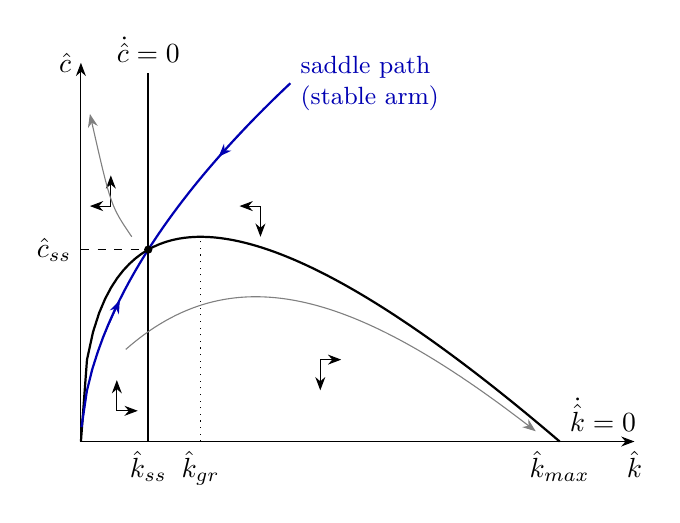
\begin{tikzpicture}[x=0.38cm,y=2.6cm,>=Stealth]
\draw[->] (0,0)--(18.5,0) node[below]{$\hat k$};
\draw[->] (0,0)--(0,1.85) node[left]{$\hat c$};
\draw[thick,domain=0:16,samples=80] plot (\x,{sqrt(\x)-0.25*\x}) node[above right]{$\dot{\hat k}=0$};
\draw[thick] (2.25,0)--(2.25,1.8) node[above]{$\dot{\hat c}=0$};
\draw[thick,blue!70!black,domain=0.02:7,samples=40] plot (\x,{0.9375*(\x/2.25)^0.55}) node[right,align=left,font=\small]{saddle path\\(stable arm)};
\draw[dashed] (0,0.9375) node[left]{$\hat c_{ss}$}--(2.25,0.9375);
\fill (2.25,0.9375) circle (1.5pt);
\node[below] at (2.25,0) {$\hat k_{ss}$}; \node[below] at (4,0) {$\hat k_{gr}$}; \node[below] at (16,0) {$\hat k_{max}$};
\draw[dotted] (4,0)--(4,1);
\draw[->,blue!70!black] (0.8,0.53)--(1.3,0.69); \draw[->,blue!70!black] (6,1.61)--(4.6,1.39);
% quadrant arrows
\draw[->] (1,1.15)--(1,1.3); \draw[->] (1,1.15)--(0.3,1.15);
\draw[->] (6,1.15)--(6,1.0);\draw[->] (6,1.15)--(5.3,1.15);
\draw[->] (1.2,0.15)--(1.2,0.3);\draw[->] (1.2,0.15)--(1.9,0.15);
\draw[->] (8,0.4)--(8,0.25);\draw[->] (8,0.4)--(8.7,0.4);
% divergent trajectories
\draw[gray,->] (1.7,1.0) .. controls (1.0,1.15) .. (0.3,1.6);
\draw[gray,->] (1.5,0.45) .. controls (5,0.9) and (9,0.75) .. (15.2,0.05);
\end{tikzpicture}
\end{center}
\emph{How to read it.} The horizontal axis is capital per effective worker, the vertical axis consumption per effective worker. The two loci split the plane into four regions. In each region the black arrows show the direction of motion: vertical arrows from the EE (up left of $\hat k_{ss}$, down right of it), horizontal arrows from the RC (left above the hump, right below it). Only paths on the blue \emph{saddle path} (stable arm) converge to the steady state; grey paths that start off it diverge.

\paragraph{Why the saddle path is the solution.} $\hat k_0$ is given, but $\hat c_0$ is free (a control can jump). We show that every starting $\hat c_0$ other than the one on the saddle path violates an optimality condition.
\begin{enumerate}
\item \textbf{Start below the saddle path} (consumption too low). The path heads right and down and eventually reaches $\hat k_{max}$ with $\hat c=0$: the saving rate equals 1. This cannot be optimal, since $u'(\hat c)=\hat c^{-\theta}\to\infty$ as $\hat c\to0$, so moving some consumption to those dates raises utility. Formally, it violates the TC. Since $\hat k_{max}>\hat k_{gr}$, the MPK there is low: $\alpha\hat k_{max}^{\alpha-1}-\delta<n+x$. Then by \eqref{rm:foc2}
\[
\frac{\dot\psi_t}{\psi_t}=-\big[\alpha\hat k_{max}^{\alpha-1}-\delta-n-x\big]>0,
\]
so $\psi_t$ does not shrink and $\lim_{t\to\infty}\psi_t\hat k_t=\lim\psi_t\hat k_{max}>0$. The household is \emph{over-saving}.
\item \textbf{Start above the saddle path} (consumption too high). The path ends up in the upper-left region where $\hat c$ rises and $\hat k$ falls. With $\hat k$ falling, rising consumption can only be financed by saving less and less. $\hat k$ hits zero in finite time, output then becomes zero, and the consumption level cannot be sustained. This \emph{violates the resource constraint} (and the Euler equation, since $\hat c$ would have to jump down).
\item \textbf{Start on the saddle path.} The economy converges to $(\hat k_{ss},\hat c_{ss})$, which lies on both loci and so satisfies the EE and the RC. It also satisfies the TC. At $\hat k_{ss}$, $\alpha\hat k_{ss}^{\alpha-1}-\delta=\rho+\theta x$, so
\[
\frac{\dot\psi_t}{\psi_t}=-\big[\rho+\theta x-n-x\big]=-\big[\rho-n-(1-\theta)x\big]=-\gamma<0 .
\]
So $\psi_t\to0$ exponentially while $\hat k_t\to\hat k_{ss}$, and $\psi_t\hat k_t\to0$.
\end{enumerate}
\begin{keybox}[title={Equilibrium path}]
Given $\hat k_0$, $\hat c_0$ jumps to the unique point on the saddle path, and the economy then moves along it monotonically to $(\hat k_{ss},\hat c_{ss})$. If $\hat k_0<\hat k_{ss}$, both $\hat k$ and $\hat c$ rise over time. This is the model's predicted development path.
\end{keybox}

%==============================================================
\subsection{Golden rule vs.\ modified golden rule \pg{31}}

The \textbf{golden rule} capital stock maximises steady-state consumption (exactly as in Solow). Steady-state consumption is output minus the investment needed to keep $\hat k$ constant:
\[
\max_{\hat k}\ \hat c=\hat y-\hat i=\hat k^\alpha-(\delta+n+x)\hat k .
\]
FOC: $\alpha\hat k^{\alpha-1}-(\delta+n+x)=0$. Solving as in \eqref{rm:kss}:
\begin{equation}
\hat k_{gr}=\Big[\frac{\alpha}{\delta+n+x}\Big]^{\frac1{1-\alpha}} . \label{rm:kgr}
\end{equation}
(The second derivative, $\alpha(\alpha-1)\hat k^{\alpha-2}<0$, confirms a maximum.)

\paragraph{Comparison with $\hat k_{ss}$.} The map $z\mapsto z^{1/(1-\alpha)}$ is increasing, so
\begin{align*}
\hat k_{gr}>\hat k_{ss}
&\iff \frac{\alpha}{\delta+n+x}>\frac{\alpha}{\delta+\rho+\theta x}
\iff \delta+\rho+\theta x>\delta+n+x\\
&\iff \rho-n-(1-\theta)x>0\iff\gamma>0,
\end{align*}
which holds by assumption \eqref{rm:gamma}.

\begin{keybox}[title={Modified golden rule: $\hat k_{ss}<\hat k_{gr}$}]
In the Ramsey steady state the net return is $\alpha\hat k_{ss}^{\alpha-1}-\delta=\rho+\theta x$, while the golden rule requires $\alpha\hat k_{gr}^{\alpha-1}-\delta=n+x$. Impatient households stop accumulating before reaching the golden rule: raising $\hat k$ further would raise consumption only in the far future, which they discount too heavily. Hence the Ramsey economy can never be dynamically inefficient (over-accumulate capital), unlike Solow with an arbitrary saving rate.
\end{keybox}

\paragraph{Co-state dynamics.} From \eqref{rm:foc2} with $r=\alpha\hat k^{\alpha-1}$, $\dfrac{\dot\psi}{\psi}=-\big[\alpha\hat k^{\alpha-1}-\delta-n-x\big]$, and by \eqref{rm:kgr}:
\begin{itemize}
\item at $\hat k=\hat k_{gr}$: $\dot\psi/\psi=0$;
\item at $\hat k<\hat k_{gr}$ (MPK high): $\dot\psi/\psi<0$, so $\psi$ shrinks;
\item at $\hat k>\hat k_{gr}$ (MPK low): $\dot\psi/\psi>0$, so $\psi$ grows.
\end{itemize}
This is why paths ending at $\hat k_{max}>\hat k_{gr}$ violate the TC, while the path ending at $\hat k_{ss}<\hat k_{gr}$ satisfies it.

%==============================================================
\subsection{Growth properties and income levels \pg{31--32}}

In the steady state, $\hat k$, $\hat y=\hat k^\alpha$ and $\hat c$ are constant. Recover per-capita and aggregate variables using ``growth rate of a product = sum of growth rates'':
\begin{align*}
\frac{Y_t}{L_t}=A_t\hat y_t\ &\Rightarrow\ \text{growth}\Big(\frac{Y}{L}\Big)=x+\underbrace{\text{growth}(\hat y)}_{0}=x,\\
Y_t=A_tL_t\hat y_t\ &\Rightarrow\ \text{growth}(Y)=x+n .
\end{align*}
The same holds for $K/L$ and $C/L$ (growth $x$) and for $K$ and $C$ (growth $x+n$).

\begin{keybox}[title={Long-run growth properties (also hold in Solow)}]
\begin{itemize}
\item Per-capita variables ($Y/L$, $K/L$, $C/L$, and the wage $w=(1-\alpha)A\hat k^\alpha$) grow at rate $x$; aggregates grow at $x+n$.
\item The capital--output ratio $K/Y=\hat k/\hat y$ is constant.
\item The rate of return to capital $r-\delta=\alpha\hat k^{\alpha-1}-\delta$ is constant. Both $K/L$ and $A$ rise over time, but they have exactly offsetting effects on the MPK.
\item Factor shares are constant: $wL/Y=1-\alpha$, $rK/Y=\alpha$.
\end{itemize}
These are consistent with the Kaldor stylised facts of long-run growth.
\end{keybox}

\paragraph{Income levels.} Output per capita on the steady-state path is
\[
\frac{Y_t}{L_t}=A_t\hat y_{ss}=A_t\hat k_{ss}^{\alpha}=\Big[\frac{\alpha}{\delta+\rho+\theta x}\Big]^{\frac{\alpha}{1-\alpha}}A_0e^{xt}.
\]
\begin{itemize}
\item Income convergence across countries requires similar $A_0$ and $x$, and, to a lesser extent, similar preference parameters $\rho,\theta$.
\item A growth ``miracle'' corresponds to a high $x$, a growth ``disaster'' to a low $x$.
\item Because the bracket varies little for plausible parameters, a factor-10 difference in income requires roughly a factor-10 difference in technology $A$.
\end{itemize}

%==============================================================
\subsection{The saving rate \pg{32--33}}

Why do the preference parameters $\rho,\theta$ affect income? Because they pin down the saving rate, which in Solow was exogenous. Define the gross saving rate $s_t\equiv\hat i_t/\hat y_t$. In the steady state, $\hat i=(\delta+n+x)\hat k_{ss}$ and $\hat y=\hat k_{ss}^\alpha$:
\begin{align*}
s_{ss}&=\frac{(\delta+n+x)\hat k_{ss}}{\hat k_{ss}^\alpha}=(\delta+n+x)\hat k_{ss}^{1-\alpha}\\
&=(\delta+n+x)\Big[\Big(\frac{\alpha}{\delta+\rho+\theta x}\Big)^{\frac1{1-\alpha}}\Big]^{1-\alpha}
&&\text{(substitute \eqref{rm:kss})}\\
&=\frac{\alpha(\delta+n+x)}{\delta+\rho+\theta x}.
\end{align*}
\begin{keybox}[title={Steady-state saving rate}]
\[
s_{ss}=\frac{\alpha(\delta+n+x)}{\delta+\rho+\theta x}\qquad(<\alpha\text{, since }\gamma>0;\ \alpha=\text{golden-rule saving rate}).
\]
\end{keybox}

\paragraph{Comparative statics} (sign of each partial derivative):
\begin{itemize}
\item $\rho$: $\dfrac{\partial s_{ss}}{\partial\rho}=-\dfrac{\alpha(\delta+n+x)}{(\delta+\rho+\theta x)^2}<0$. Households discount the future more heavily (the factor $e^{-\rho t}$ falls), so they are less willing to save.
\item $\theta$: $\dfrac{\partial s_{ss}}{\partial\theta}=-\dfrac{\alpha(\delta+n+x)\,x}{(\delta+\rho+\theta x)^2}<0$ (for $x>0$). A larger $\theta$ means more curvature in $u$ and a stronger desire to smooth consumption. Since consumption per capita grows at $x$, smoothing means shifting consumption toward the present, so households save less.
\item $n$: $\dfrac{\partial s_{ss}}{\partial n}=\dfrac{\alpha}{\delta+\rho+\theta x}>0$. Note that $\hat k_{ss}$ and $\hat y_{ss}$ do not depend on $n$ (see \eqref{rm:kss}), so the MPK in steady state is unaffected. The saving rate rises because more investment, $(\delta+n+x)\hat k_{ss}$, is needed just to equip the new workers and keep $\hat k$ at $\hat k_{ss}$ (``capital widening'').
\end{itemize}

\paragraph{Transitional dynamics of the saving rate.} Along the saddle path (say $\hat k_0<\hat k_{ss}$), $s_t$ may rise or fall toward $s_{ss}$, because two effects push in opposite directions:
\begin{itemize}
\item \textbf{Substitution effect (SE):} as $\hat k\uparrow$, the return $MPK-\delta$ falls, so saving becomes less rewarding and $s_t\downarrow$.
\item \textbf{Income effect (IE):} households want a reasonably flat profile for $\hat c$. Early in development, income $\hat y$ is low relative to its future level, so they consume a large share of it. As $\hat y$ rises, $\hat c$ rises more slowly than $\hat y$, so $\hat c/\hat y\downarrow$, i.e.\ $s_t=\hat i/\hat y\uparrow$.
\end{itemize}
The parameter $\theta$ governs the strength of the IE. A high $\theta$ (strong smoothing motive) gives a large IE: the initial consumption share $\hat c/\hat y$ is high and falls over time, so $s_t$ rises during the transition. (Barro--Sala-i-Martin, Cobb--Douglas case: $s_t$ is constant if $s_{ss}=1/\theta$, rises over the transition if $s_{ss}>1/\theta$, and falls if $s_{ss}<1/\theta$.)

%==============================================================
\subsection{Fiscal policy I: lump-sum tax \pg{33--34}}

\paragraph{Setup.} Add a government to the baseline model.
\begin{itemize}
\item $G_t$: government spending. It is \emph{completely wasteful}: it enters neither the utility function nor the production function.
\item $T_t$: aggregate tax revenue, raised \emph{lump-sum} (the amount paid does not depend on any household choice).
\item Balanced budget: $T_t=G_t$. Per effective worker, $\tau\equiv T_t/(A_tL_t)$ and $\hat g\equiv G_t/(A_tL_t)$, so $\tau=\hat g$ for all $t$.
\item Firms face the same problem as before, so $r_t,w_t$ are still given by \eqref{rm:r}--\eqref{rm:w}.
\end{itemize}

\paragraph{Household problem.} Same objective, but taxes reduce resources:
\[
\max\int_0^\infty\frac{\hat c_t^{1-\theta}}{1-\theta}e^{-\gamma t}dt\quad\text{s.t.}\quad
\dot{\hat k}_t=\frac{w_t}{A_t}+(r_t-\delta-n-x)\hat k_t-\hat c_t-\tau .
\]
The Hamiltonian adds the term $-\psi_t\tau$. Because $\tau$ depends on neither $\hat c_t$ nor $\hat k_t$, the derivatives $\partial\mathcal H/\partial\hat c$ and $\partial\mathcal H/\partial\hat k$ are unchanged. Conditions \eqref{rm:foc1}--\eqref{rm:foc2}, and hence the Euler equation, are exactly as in the baseline. Using \eqref{rm:exhaust} and $\tau=\hat g$ in the budget constraint:
\begin{align}
\frac{\dot{\hat c}_t}{\hat c_t}&=\frac1\theta\big[\alpha\hat k_t^{\alpha-1}-\delta-\rho-\theta x\big] &&\text{(same as baseline)}, \label{rm:EEls}\\
\dot{\hat k}_t&=\hat k_t^\alpha-(\delta+n+x)\hat k_t-\hat c_t-\hat g &&\text{(one extra term, $-\hat g$)}. \label{rm:RCls}
\end{align}

\paragraph{Steady state.} $\dot{\hat c}=0$ in \eqref{rm:EEls} gives the same $\hat k_{ss}=\big[\frac{\alpha}{\delta+\rho+\theta x}\big]^{\frac1{1-\alpha}}$ as \eqref{rm:kss}. $\dot{\hat k}=0$ in \eqref{rm:RCls} gives
\[
\hat c_{ss}=\hat k_{ss}^\alpha-(\delta+n+x)\hat k_{ss}-\hat g .
\]

\begin{center}
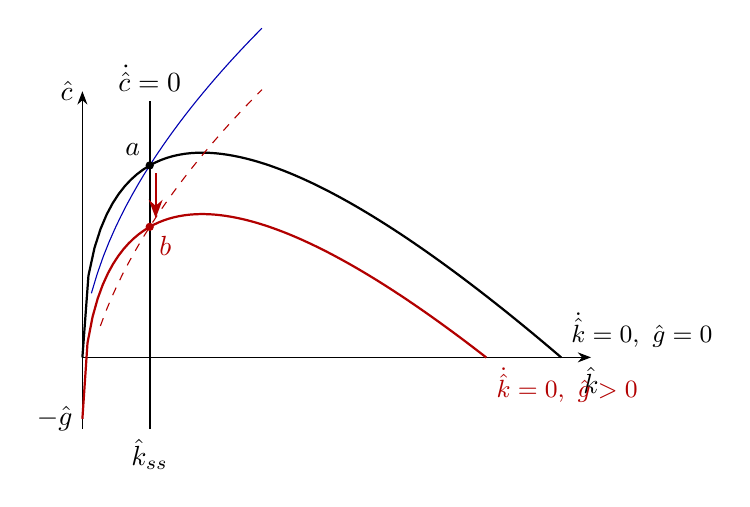
\begin{tikzpicture}[x=0.38cm,y=2.6cm,>=Stealth]
\draw[->] (0,0)--(17,0) node[below]{$\hat k$};
\draw[->] (0,-0.35)--(0,1.3) node[left]{$\hat c$};
\draw[thick,domain=0:16,samples=80] plot (\x,{sqrt(\x)-0.25*\x}) node[above right,font=\small]{$\dot{\hat k}=0,\ \hat g=0$};
\draw[thick,red!70!black,domain=0:13.5,samples=80] plot (\x,{sqrt(\x)-0.25*\x-0.3}) node[below right,font=\small]{$\dot{\hat k}=0,\ \hat g>0$};
\draw[thick] (2.25,-0.35)--(2.25,1.25) node[above]{$\dot{\hat c}=0$};
\draw[blue!70!black,domain=0.3:6,samples=30] plot (\x,{0.9375*(\x/2.25)^0.55});
\draw[red!70!black,dashed,domain=0.6:6,samples=30] plot (\x,{0.9375*(\x/2.25)^0.55-0.3});
\fill (2.25,0.9375) circle (1.5pt) node[above left]{$a$};
\fill[red!70!black] (2.25,0.6375) circle (1.5pt) node[below right]{$b$};
\draw[->,thick,red!70!black] (2.45,0.9)--(2.45,0.68);
\node[left] at (0,-0.3) {$-\hat g$};
\node[below] at (2.25,-0.35) {$\hat k_{ss}$};
\end{tikzpicture}
\end{center}
\emph{How to read it.} The black hump is the baseline $\dot{\hat k}=0$ locus; the red hump is the same curve shifted down by $\hat g$ at every $\hat k$ (a parallel shift, starting at $-\hat g$ on the vertical axis). The vertical $\dot{\hat c}=0$ line does not move, because the Euler equation is unchanged. The steady state moves straight down from $a$ to $b$. The solid blue and dashed red curves are the old and new saddle paths.

\begin{keybox}[title={Permanent rise in a lump-sum tax ($\hat g=0\to\hat g>0$)}]
The tax is a pure drain on wealth. The $\dot{\hat k}=0$ locus shifts down in parallel by $\hat g$; the $\dot{\hat c}=0$ locus does not move. At the moment of the change, $\hat k=\hat k_{ss}$ is already at the new steady-state value, so $\hat c$ jumps immediately from $a$ to $b$, falling one-for-one with the tax. There are no transitional dynamics: short-run effect = long-run effect. $\hat k_{ss}$, and therefore income $\hat y_{ss}$, are unaffected by $\hat g$. Foreign aid is a negative lump-sum tax: a parallel shift \emph{up}, and $\hat c$ jumps up by the amount of aid.
\end{keybox}
\begin{tipbox}
Lump-sum taxes do not change the after-tax return to capital, so the saving incentive (the EE) is untouched. To smooth consumption, the household absorbs the whole permanent tax at once by cutting $\hat c$ by exactly $\tau$. Does the ``taxes don't affect income'' result survive distortionary taxation? No, as shown next.
\end{tipbox}

%==============================================================
\subsection{Fiscal policy II: proportional income tax \pg{34--36}}

\paragraph{Setup.} Now the government taxes all income (wages and capital rentals) at a constant rate $\tau\in[0,1]$. Spending $G_t$ is still wasteful.
\begin{itemize}
\item \textbf{Firms:} unchanged, $w_t=(1-\alpha)Y_t/L_t=(1-\alpha)A_t\hat k_t^\alpha$ and $r_t=\alpha Y_t/K_t=\alpha\hat k_t^{\alpha-1}$.
\item \textbf{Government:} $\tau(w_tL_t+r_tK_t)=G_t$. Divide both sides by $A_tL_t$ and use \eqref{rm:exhaust}:
\[
\tau\Big(\frac{w_t}{A_t}+r_t\hat k_t\Big)=\hat g_t\ \Longrightarrow\ \hat g_t=\tau\hat y_t=\tau\hat k_t^{\alpha}.
\]
\item \textbf{Households:} after-tax income is $(1-\tau)(w_tL_t+r_tK_t)$. Repeating the steps behind \eqref{rm:bc}:
\begin{equation}
\dot{\hat k}_t=(1-\tau)\frac{w_t}{A_t}+\big[(1-\tau)r_t-\delta-n-x\big]\hat k_t-\hat c_t . \label{rm:bcpt}
\end{equation}
Depreciation is not tax-deductible here: the household earns $(1-\tau)r_t$ and loses $\delta$.
\end{itemize}

\paragraph{Optimality.} The Hamiltonian is
\[
\mathcal H_t=\frac{\hat c_t^{1-\theta}}{1-\theta}e^{-\gamma t}+\psi_t\Big[(1-\tau)\frac{w_t}{A_t}+\big[(1-\tau)r_t-\delta-n-x\big]\hat k_t-\hat c_t\Big].
\]
(As before, the constraint enters only through $\psi_t$ times its right-hand side, much like a Lagrange multiplier.) Conditions:
\begin{align}
\frac{\partial\mathcal H_t}{\partial\hat c_t}=0:&\qquad \hat c_t^{-\theta}e^{-\gamma t}=\psi_t, \label{rm:pt1}\\
-\frac{\partial\mathcal H_t}{\partial\hat k_t}=\dot\psi_t:&\qquad \frac{\dot\psi_t}{\psi_t}=-\big[(1-\tau)r_t-\delta-n-x\big], \label{rm:pt2}
\end{align}
plus \eqref{rm:bcpt} and the TC $\lim_{t\to\infty}\psi_t\hat k_t=0$. Differentiating \eqref{rm:pt1} gives $\dot\psi_t/\psi_t=-\theta\dot{\hat c}_t/\hat c_t-\gamma$ (same steps as before). Equating with \eqref{rm:pt2}:
\begin{align*}
\theta\frac{\dot{\hat c}_t}{\hat c_t}&=(1-\tau)r_t-\delta-n-x-\gamma=(1-\tau)r_t-\delta-\rho-\theta x .
\end{align*}
For the capital equation, substitute the firm conditions into \eqref{rm:bcpt}:
\begin{align*}
\dot{\hat k}_t&=(1-\tau)(1-\alpha)\hat k_t^\alpha+(1-\tau)\alpha\hat k_t^{\alpha}-(\delta+n+x)\hat k_t-\hat c_t\\
&=(1-\tau)\hat k_t^\alpha-(\delta+n+x)\hat k_t-\hat c_t .
\end{align*}
(Equivalently: output $\hat k^\alpha$ = $\hat c+\hat i+\hat g$ with $\hat g=\tau\hat k^\alpha$.)

\begin{keybox}[title={Ramsey model with a proportional income tax}]
\begin{align}
\frac{\dot{\hat c}_t}{\hat c_t}&=\frac1\theta\big[(1-\tau)\alpha\hat k_t^{\alpha-1}-\delta-\rho-\theta x\big], \label{rm:EEpt}\\
\dot{\hat k}_t&=(1-\tau)\hat k_t^\alpha-(\delta+n+x)\hat k_t-\hat c_t . \label{rm:RCpt}
\end{align}
Steady state (solve \eqref{rm:EEpt}$=0$ exactly as for \eqref{rm:kss}, with $\alpha$ replaced by $\alpha(1-\tau)$):
\[
\hat k_{ss}=\Big[\frac{\alpha(1-\tau)}{\delta+\rho+\theta x}\Big]^{\frac1{1-\alpha}},\qquad
\hat c_{ss}=(1-\tau)\hat k_{ss}^\alpha-(\delta+n+x)\hat k_{ss}.
\]
\end{keybox}

\begin{center}
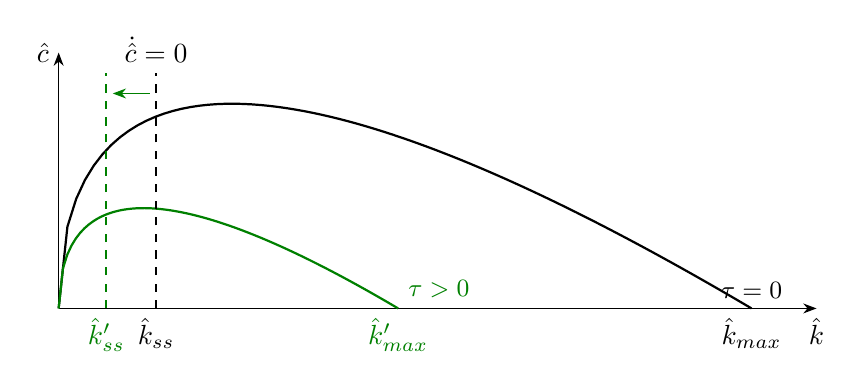
\begin{tikzpicture}[x=0.55cm,y=2.6cm,>=Stealth]
\draw[->] (0,0)--(17.5,0) node[below]{$\hat k$};
\draw[->] (0,0)--(0,1.25) node[left]{$\hat c$};
\draw[thick,domain=0:16,samples=80] plot (\x,{sqrt(\x)-0.25*\x}) node[above,font=\small]{$\tau=0$};
\draw[thick,green!50!black,domain=0:7.84,samples=80] plot (\x,{0.7*sqrt(\x)-0.25*\x}) node[above right,font=\small]{$\tau>0$};
\draw[dashed,thick] (2.25,0)--(2.25,1.15) node[above]{$\dot{\hat c}=0$};
\draw[dashed,thick,green!50!black] (1.1,0)--(1.1,1.15);
\draw[->,green!50!black] (2.1,1.05)--(1.25,1.05);
\node[below] at (2.25,0) {$\hat k_{ss}$}; \node[below,green!50!black] at (1.1,0) {$\hat k_{ss}'$};
\node[below] at (16,0) {$\hat k_{max}$}; \node[below,green!50!black] at (7.84,0) {$\hat k_{max}'$};
\end{tikzpicture}
\end{center}
\emph{How to read it.} Black curves are for $\tau=0$, green curves for $\tau>0$. The vertical $\dot{\hat c}=0$ line shifts left (from $\hat k_{ss}$ to $\hat k'_{ss}$) because the after-tax return is lower. The $\dot{\hat k}=0$ hump falls by $\tau\hat k^\alpha$. This gap is small at low $\hat k$ and grows with $\hat k$, so the shift is \emph{not} parallel, and the right intercept $\hat k_{max}=\big[(1-\tau)/(\delta+n+x)\big]^{1/(1-\alpha)}$ also moves left.

\paragraph{Two effects of a tax increase.}
\begin{enumerate}
\item \textbf{Distortion of the return to capital.} The after-tax MPK $(1-\tau)\alpha\hat k^{\alpha-1}$ falls, so the $\dot{\hat c}=0$ locus shifts left: $\hat k_{ss}\downarrow$. The saving rate also falls:
\[
s_{ss}=(\delta+n+x)\hat k_{ss}^{1-\alpha}=\frac{\alpha(1-\tau)(\delta+n+x)}{\delta+\rho+\theta x}.
\]
\item \textbf{Lower disposable income.} The $\dot{\hat k}=0$ locus shifts down, non-parallel, as described above.
\end{enumerate}
\begin{keybox}[title={Proportional vs.\ lump-sum taxation}]
Unlike the lump-sum case, a proportional tax lowers long-run capital and income, $\hat y_{ss}=\hat k_{ss}^\alpha$, because it distorts the saving decision. After a permanent increase in $\tau$, $\hat k$ cannot jump. $\hat c$ jumps onto the new saddle path (up or down, depending on whether the substitution or the income effect dominates), and then $\hat k$ and $\hat c$ decline gradually toward the new, lower steady state. So, unlike the lump-sum case, there are transitional dynamics.
\end{keybox}

\paragraph{Revenue and the Laffer curve.} In steady state the revenue per effective worker is
\[
\hat g^*=\tau\hat y^*=\tau\hat k_{ss}^\alpha=\tau\Big[\frac{\alpha(1-\tau)}{\delta+\rho+\theta x}\Big]^{\frac{\alpha}{1-\alpha}}.
\]
\begin{enumerate}[label=(\roman*)]
\item $\tau=0\Rightarrow\hat g^*=0$: no tax, no revenue.
\item $\tau=1\Rightarrow\hat g^*=0$: with a 100\% tax there is no disposable income, hence no investment, so $\hat k_{ss}=0$ and there is no output in the long run.
\item $0<\tau<1\Rightarrow\hat g^*>0$.
\end{enumerate}
So revenue is hump-shaped in $\tau$. Which $\tau$ maximises it? Write $a\equiv\frac{\alpha}{1-\alpha}$ and $B\equiv\big[\frac{\alpha}{\delta+\rho+\theta x}\big]^{a}>0$, so $\hat g^*=B\,\tau(1-\tau)^{a}$. By the product rule:
\begin{align*}
\frac{d\hat g^*}{d\tau}&=B\Big[(1-\tau)^{a}+\tau\cdot a(1-\tau)^{a-1}\cdot(-1)\Big]\\
&=B(1-\tau)^{a-1}\big[(1-\tau)-a\tau\big]
&&\text{(factor out $(1-\tau)^{a-1}$)}.
\end{align*}
Set it to zero (for $\tau<1$, $B(1-\tau)^{a-1}>0$, so the bracket must vanish):
\begin{align*}
1-\tau&=\frac{\alpha}{1-\alpha}\tau\\
(1-\alpha)(1-\tau)&=\alpha\tau &&\text{(multiply by $1-\alpha$)}\\
1-\alpha-\tau+\alpha\tau&=\alpha\tau\\
\tau&=1-\alpha .
\end{align*}
The bracket is positive for $\tau<1-\alpha$ and negative for $\tau>1-\alpha$, so this is a maximum. The constant $B$ dropped out.

\begin{center}
\begin{tikzpicture}[x=5cm,y=7cm,>=Stealth]
\draw[->] (0,0)--(1.1,0) node[below]{$\tau$};
\draw[->] (0,0)--(0,0.48) node[left]{$\hat g^*$};
\draw[thick,domain=0:1,samples=80] plot (\x,{\x*sqrt(1-\x)});
\draw[dashed] (0.6667,0)--(0.6667,0.3849);
\node[below] at (0.6667,0) {$1-\alpha$};
\node[below] at (1,0) {$1$}; \node[below left] at (0,0) {$0$};
\end{tikzpicture}
\end{center}
\emph{How to read it.} The horizontal axis is the tax rate, the vertical axis steady-state revenue (drawn for $\alpha=1/3$). Revenue is zero at both ends. Raising $\tau$ above $1-\alpha$ shrinks the tax base $\hat y^*$ so much that revenue falls: this is the wrong side of the Laffer curve.

\begin{keybox}[title={Revenue-maximising tax rate}]
\[
\tau^*=1-\alpha\qquad(\text{the labour share}).
\]
\end{keybox}

%==============================================================
\subsection{Infrastructure (productive public capital) in the Ramsey model \pg{36--37}}

\paragraph{Setup.} The government taxes income at rate $\tau$ and spends the revenue on infrastructure, which raises firms' productivity.
\begin{itemize}
\item \textbf{No technological change:} $A$ is a constant ($x=0$, no $A_0e^{xt}$). We therefore work in \emph{per-capita} terms (no hats): $k_t=K_t/L_t$, $c_t=C_t/L_t$, $y_t=Y_t/L_t$.
\item $g_t$: productive government services per capita. Firms and households take it as given.
\item $\beta\in(0,1)$: elasticity of output with respect to $g$. We assume $\alpha+\beta<1$ (relaxed in the next subsection).
\item Other notation as before; $\rho>n$ so that utility is finite.
\end{itemize}

\paragraph{Households.} With $x=0$ the effective discount rate \eqref{rm:gamma} becomes $\rho-n$. Per capita, the budget constraint (same steps as \eqref{rm:bcpt} with $x=0$) is
\[
\max\int_0^\infty\frac{c_t^{1-\theta}}{1-\theta}e^{-(\rho-n)t}dt\quad\text{s.t.}\quad
\dot k_t=(1-\tau)w_t+\big[(1-\tau)r_t-\delta-n\big]k_t-c_t .
\]
Hamiltonian:
\[
\mathcal H_t=\frac{c_t^{1-\theta}}{1-\theta}e^{-(\rho-n)t}+\psi_t\Big[(1-\tau)w_t+\big((1-\tau)r_t-\delta-n\big)k_t-c_t\Big].
\]
Conditions:
\begin{align}
c_t^{-\theta}e^{-(\rho-n)t}&=\psi_t, \label{rm:in1}\\
\dot\psi_t&=-\big[(1-\tau)r_t-\delta-n\big]\psi_t,\qquad \lim_{t\to\infty}\psi_tk_t=0, \label{rm:in2}\\
\dot k_t&=(1-\tau)w_t+\big[(1-\tau)r_t-\delta-n\big]k_t-c_t . \label{rm:in3}
\end{align}
Differentiate \eqref{rm:in1} with respect to $t$ and divide by $\psi_t$: $\dot\psi_t/\psi_t=-\theta\dot c_t/c_t-(\rho-n)$. Equate with \eqref{rm:in2}:
\begin{align*}
-\theta\frac{\dot c_t}{c_t}-(\rho-n)&=-\big[(1-\tau)r_t-\delta-n\big]\\
\theta\frac{\dot c_t}{c_t}&=(1-\tau)r_t-\delta-n-\rho+n=(1-\tau)r_t-\delta-\rho,
\end{align*}
\begin{equation}
\frac{\dot c_t}{c_t}=\frac1\theta\big[(1-\tau)r_t-\delta-\rho\big]. \label{rm:in4}
\end{equation}

\paragraph{Firms.} $\max\{Y_t-w_tL_t-r_tK_t\}$ s.t.
\begin{equation}
Y_t=AL_t^{1-\alpha}K_t^\alpha g_t^\beta\quad\Longleftrightarrow\quad y_t=Ak_t^\alpha g_t^\beta\quad\text{(divide by $L_t$)}. \label{rm:in5}
\end{equation}
For given $g_t$ there are constant returns in $(K,L)$, so factor payments exhaust output. FOCs:
\begin{align}
w_t&=\frac{\partial Y_t}{\partial L_t}=(1-\alpha)AL_t^{-\alpha}K_t^\alpha g_t^\beta=(1-\alpha)\underbrace{Ak_t^\alpha g_t^\beta}_{y_t}=(1-\alpha)y_t, \label{rm:in6}\\
r_t&=\frac{\partial Y_t}{\partial K_t}=\alpha Ak_t^{\alpha-1}g_t^\beta=\alpha\frac{y_t}{k_t}. \label{rm:in7}
\end{align}
Hence $w_t+r_tk_t=(1-\alpha)y_t+\alpha y_t=y_t$.

\paragraph{Government.} Balanced budget, all revenue spent on infrastructure:
\begin{equation}
G_t=\tau(w_tL_t+r_tK_t)=\tau Y_t\ \Longrightarrow\ g_t=\frac{G_t}{L_t}=\tau y_t . \label{rm:in8}
\end{equation}

\paragraph{Reduced form.} Substitute \eqref{rm:in8} into \eqref{rm:in5} and solve for $y_t$:
\begin{align}
y_t&=Ak_t^\alpha(\tau y_t)^\beta=A\tau^\beta k_t^\alpha y_t^\beta \notag\\
y_t^{1-\beta}&=A\tau^\beta k_t^\alpha &&\text{(divide by $y_t^\beta$)} \notag\\
y_t&=A^{\frac1{1-\beta}}\tau^{\frac{\beta}{1-\beta}}k_t^{\frac{\alpha}{1-\beta}} &&\text{(raise to the power $\tfrac1{1-\beta}$).} \label{rm:in9}
\end{align}
Then from \eqref{rm:in7}:
\begin{equation}
r_t=\alpha\frac{y_t}{k_t}=\alpha A^{\frac1{1-\beta}}\tau^{\frac{\beta}{1-\beta}}k_t^{\frac{\alpha}{1-\beta}-1}
=\alpha A^{\frac1{1-\beta}}\tau^{\frac{\beta}{1-\beta}}k_t^{\frac{\alpha+\beta-1}{1-\beta}}, \label{rm:in10}
\end{equation}
using $\frac{\alpha}{1-\beta}-1=\frac{\alpha-(1-\beta)}{1-\beta}$. With $\alpha+\beta<1$ the exponent is negative, so the private return to capital still diminishes in $k$.

\paragraph{Dynamic system.} Use $w_t+r_tk_t=y_t$ in \eqref{rm:in3}, i.e.\ $(1-\tau)w_t+(1-\tau)r_tk_t=(1-\tau)y_t$, then \eqref{rm:in9}. For the EE, use \eqref{rm:in10} in \eqref{rm:in4}.
\begin{keybox}[title={Infrastructure model}]
\begin{align*}
\text{RC:}\quad \dot k_t&=(1-\tau)y_t-(\delta+n)k_t-c_t\\
&=(1-\tau)A^{\frac1{1-\beta}}\tau^{\frac{\beta}{1-\beta}}k_t^{\frac{\alpha}{1-\beta}}-(\delta+n)k_t-c_t,\\
\text{EE:}\quad \frac{\dot c_t}{c_t}&=\frac1\theta\Big[(1-\tau)\alpha A^{\frac1{1-\beta}}\tau^{\frac{\beta}{1-\beta}}k_t^{\frac{\alpha+\beta-1}{1-\beta}}-\delta-\rho\Big].
\end{align*}
\end{keybox}
This has the same structure as the proportional-tax model, with output $\propto k^{\alpha/(1-\beta)}$ instead of $\hat k^\alpha$. The phase diagram looks the same.

\paragraph{Steady state} ($\dot c=\dot k=0$). Let $\Phi(\tau)\equiv(1-\tau)\tau^{\frac{\beta}{1-\beta}}$. Setting the EE bracket to zero:
\begin{align*}
\alpha\,\Phi(\tau)A^{\frac1{1-\beta}}k_{ss}^{\frac{\alpha+\beta-1}{1-\beta}}&=\delta+\rho\\
k_{ss}^{-\frac{1-\alpha-\beta}{1-\beta}}&=\frac{\delta+\rho}{\alpha\Phi(\tau)A^{\frac1{1-\beta}}}\\
k_{ss}&=\Big[\frac{\alpha\Phi(\tau)A^{\frac1{1-\beta}}}{\delta+\rho}\Big]^{\frac{1-\beta}{1-\alpha-\beta}}
&&\text{(raise to the power $-\tfrac{1-\beta}{1-\alpha-\beta}$).}
\end{align*}
\begin{keybox}[title={Steady state with infrastructure (requires $\alpha+\beta<1$)}]
\begin{align}
k_{ss}&=\Big[\frac{\alpha(1-\tau)\tau^{\frac{\beta}{1-\beta}}A^{\frac1{1-\beta}}}{\delta+\rho}\Big]^{\frac{1-\beta}{1-\alpha-\beta}}, \label{rm:in11}\\
c_{ss}&=(1-\tau)\tau^{\frac{\beta}{1-\beta}}A^{\frac1{1-\beta}}k_{ss}^{\frac{\alpha}{1-\beta}}-(\delta+n)k_{ss}. \label{rm:in12}
\end{align}
\end{keybox}

\paragraph{Effect of $\tau$ on $k_{ss}$.} It is not obvious, because the tax works in two directions: it finances productive $g$ (good for the return to capital) and it lowers the after-tax return (bad). The outer exponent $\frac{1-\beta}{1-\alpha-\beta}$ is positive, so $k_{ss}$ moves in the same direction as $\Phi(\tau)$. Differentiate $\Phi$ with the product rule:
\begin{align*}
\Phi'(\tau)&=-\tau^{\frac{\beta}{1-\beta}}+\frac{\beta}{1-\beta}(1-\tau)\tau^{\frac{\beta}{1-\beta}-1}\\
&=\frac{\tau^{\frac{\beta}{1-\beta}-1}}{1-\beta}\Big[-(1-\beta)\tau+\beta(1-\tau)\Big]
&&\text{(factor out $\tfrac{1}{1-\beta}\tau^{\frac{\beta}{1-\beta}-1}$)}\\
&=\frac{\tau^{\frac{\beta}{1-\beta}-1}}{1-\beta}\,(\beta-\tau)
&&\text{($-\tau+\beta\tau+\beta-\beta\tau=\beta-\tau$).}
\end{align*}
The prefactor is positive, so $\operatorname{sign}\Phi'(\tau)=\operatorname{sign}(\beta-\tau)$.
\begin{keybox}[title={Tax and steady-state capital with productive spending}]
\begin{itemize}
\item $\tau<\beta$: $\Phi'>0$, so raising $\tau$ \emph{raises} $k_{ss}$. Infrastructure is scarce and its productivity gain dominates.
\item $\tau>\beta$: $\Phi'<0$, so raising $\tau$ \emph{lowers} $k_{ss}$. The distortion of the after-tax return dominates.
\item $k_{ss}$ (and hence $y_{ss}$) is maximised at $\tau=\beta$: set the tax share equal to the output elasticity of public services (natural efficiency condition $\partial Y/\partial G=1$, since $\partial Y/\partial G=\beta Y/G=\beta/\tau$).
\end{itemize}
\end{keybox}

%==============================================================
\subsection{Endogenous growth: the AK case $\beta=1-\alpha$ \pg{38}}

\paragraph{Setup.} Same model, but now $\alpha+\beta=1$, i.e.\ $\beta=1-\alpha$. Then
\[
\frac1{1-\beta}=\frac1\alpha,\qquad \frac{\beta}{1-\beta}=\frac{1-\alpha}{\alpha},\qquad \frac{\alpha}{1-\beta}=1,\qquad \frac{\alpha+\beta-1}{1-\beta}=0 .
\]
Substitute into \eqref{rm:in9}--\eqref{rm:in10}:
\[
y_t=\underbrace{A^{\frac1\alpha}\tau^{\frac{1-\alpha}{\alpha}}}_{\equiv\tilde A}\,k_t\quad(\text{linear in }k:\ \text{an ``AK'' technology}),\qquad
r_t=\alpha\tilde A\quad(\text{constant}).
\]
Because the government expands $g$ in proportion to output, the return to private capital no longer diminishes as $k$ grows.

\paragraph{Dynamics.} The EE \eqref{rm:in4} becomes
\[
\frac{\dot c_t}{c_t}=\frac1\theta\Big[(1-\tau)\alpha A^{\frac1\alpha}\tau^{\frac{1-\alpha}{\alpha}}-\delta-\rho\Big]\equiv\gamma_c\qquad\text{(a constant)}.
\]
Here $\gamma_c$ denotes the consumption growth rate, not the effective discount rate $\gamma$ of \eqref{rm:gamma}. Assume $\gamma_c>0$, i.e.\ $(1-\tau)\alpha\tilde A>\delta+\rho$. Divide the RC $\dot k_t=(1-\tau)\tilde Ak_t-(\delta+n)k_t-c_t$ by $k_t$:
\[
\frac{\dot k_t}{k_t}=(1-\tau)A^{\frac1\alpha}\tau^{\frac{1-\alpha}{\alpha}}-(\delta+n)-\frac{c_t}{k_t}.
\]
So $\dot c/c$ is constant, while $\dot k/k$ is a decreasing linear function of the ratio $c/k$.

\begin{center}
\begin{tikzpicture}[x=1cm,y=1cm,>=Stealth]
\draw[->] (0,-1.2)--(0,3) node[left]{$\frac{\dot c}{c},\ \frac{\dot k}{k}$};
\draw[->] (0,0)--(5.5,0) node[below]{$\frac ck$};
\draw[thick] (0,1.2)--(5,1.2) node[right]{$\frac{\dot c}{c}=\gamma_c$};
\draw[thick,blue!70!black] (0,2.6)--(3.8,-1.2) node[right]{$\frac{\dot k}{k}$};
\node[left,font=\small] at (0,2.6) {$(1-\tau)\frac yk-\delta-n$};
\draw[dashed] (1.4,1.2)--(1.4,0) node[below]{$(\frac ck)^*$};
\draw[->,blue!70!black] (0.9,1.7)--(0.4,2.2);
\draw[->,blue!70!black] (2.0,0.6)--(2.6,0.0);
\end{tikzpicture}
\end{center}
\emph{How to read it.} The horizontal axis is the consumption--capital ratio, the vertical axis growth rates. The flat line is consumption growth $\gamma_c$, which does not depend on $c/k$. The downward-sloping line is capital growth: more consumption out of a given capital stock leaves less for investment. Its intercept is $(1-\tau)\frac yk-\delta-n$ with $\frac yk=\tilde A$. They cross at $(c/k)^*$, where $c$ and $k$ grow at the same rate. The arrows show that $c/k$ moves away from the crossing.

\paragraph{Instability of $c/k$ away from $(c/k)^*$.} Setting $\gamma_c=(1-\tau)\tilde A-(\delta+n)-(c/k)^*$ defines
\[
\Big(\frac ck\Big)^*=(1-\tau)\tilde A-(\delta+n)-\gamma_c .
\]
The growth rate of a ratio is the difference of growth rates, so
\begin{align*}
\frac{d}{dt}\ln\frac{c_t}{k_t}&=\frac{\dot c_t}{c_t}-\frac{\dot k_t}{k_t}
=\gamma_c-\Big[(1-\tau)\tilde A-(\delta+n)-\frac{c_t}{k_t}\Big]
=\frac{c_t}{k_t}-\Big(\frac ck\Big)^* .
\end{align*}
\begin{itemize}
\item If $\frac ck<(\frac ck)^*$: $c/k$ falls and keeps falling toward 0. Consumption is too low and capital piles up, so the value of capital does not vanish: this \emph{violates the TC}.
\item If $\frac ck>(\frac ck)^*$: $c/k$ rises without bound. Consumption grows faster than output can support, $k$ eventually hits zero: this \emph{violates the RC}.
\end{itemize}
(For the TC to hold on the balanced path we need $(c/k)^*>0$, i.e.\ $(1-\tau)\tilde A-\delta-n>\gamma_c$.)

\begin{keybox}[title={AK growth with productive government: no transitional dynamics}]
The only optimal choice is for $c_0$ to jump so that $c_0/k_0=(c/k)^*$ immediately. From then on $c$, $k$ and $y=\tilde Ak$ all grow at the same constant rate
\[
\gamma_c=\frac1\theta\Big[(1-\tau)\alpha A^{\frac1\alpha}\tau^{\frac{1-\alpha}{\alpha}}-\delta-\rho\Big]
\]
forever. The ``steady state'' is now a constant \emph{growth rate} (balanced growth), not $\dot c=\dot k=0$ as in the baseline. Long-run growth is \emph{endogenous}: policy ($\tau$) and preferences ($\rho,\theta$) affect the growth rate, not just income levels. Growth is maximised where $(1-\tau)\tau^{\frac{1-\alpha}{\alpha}}=\Phi(\tau)$ peaks. By the derivative computed above with $\beta=1-\alpha$, this is at $\tau=\beta=1-\alpha$.
\end{keybox}
\begin{tipbox}
Compare: with $\alpha+\beta<1$, taxes for infrastructure change the \emph{level} of $k_{ss}$ (maximised at $\tau=\beta$). With $\alpha+\beta=1$, the same tax changes the \emph{growth rate} (also maximised at $\tau=\beta$). The knife-edge $\alpha+\beta=1$ removes diminishing returns to the accumulable factor, which is what makes growth endogenous.
\end{tipbox}

\section{Tools: Dynamic Programming, Continuous-Time Stochastic Processes, Markov Chains}

This section collects the mathematical tools used throughout the course: (i) dynamic programming in continuous time (the Hamilton--Jacobi--Bellman, or HJB, equation), with and without uncertainty; (ii) the Kolmogorov forward equation for the evolution of a distribution; (iii) Brownian motion and its relatives; (iv) It\^o's lemma; (v) discrete Markov chains.

%=====================================================================
\subsection{Overview: three forms of the HJB equation \pg{11--12}}

\paragraph{Notation used in this subsection.}
\begin{itemize}
\item $t$: time (continuous); $T$: terminal date ($T=\infty$ for an infinite horizon).
\item $x$: \emph{state variable} (e.g.\ wealth or capital). It is given at each instant and can only be changed gradually.
\item $u$: \emph{control variable} (e.g.\ consumption). The agent chooses it at each instant.
\item $f(x,u,t)$: flow return (instantaneous payoff, e.g.\ utility of consumption).
\item $g(x,u,t)$: law of motion of the state, $\dot x\equiv dx/dt=g(x,u,t)$ (e.g.\ the budget constraint).
\item $\rho>0$: subjective discount rate.
\item $V$: value function, the maximal attainable value of the objective starting from a given state (and date). Subscripts denote partial derivatives: $V_t=\partial V/\partial t$, $V_x=\partial V/\partial x$, $V_{xx}=\partial^2V/\partial x^2$; $V'(x)$ is the ordinary derivative when $V$ depends on $x$ only.
\item $W_t$: standard Brownian motion (defined in Section~\ref{sec:sbm}); $dW_t$ is its increment.
\item $\mu(x,u)$, $\sigma(x)$: drift and volatility of the state when it is stochastic, $dx=\mu(x,u)\,dt+\sigma(x)\,dW$.
\end{itemize}

\begin{keybox}[title=Three forms of the HJB equation]
\begin{itemize}
\item \textbf{Classic HJB} (deterministic, time-dependent, typically finite horizon; a partial differential equation (PDE) in $(x,t)$):
\begin{equation}\label{eq:hjb-classic}
-V_t(x,t)=\max_u\big\{f(x,u,t)+V_x(x,t)\,g(x,u,t)\big\}.
\end{equation}
\item \textbf{Stationary HJB} (deterministic, infinite horizon, time enters only through discounting at rate $\rho$; an ordinary differential equation (ODE) in $x$ only):
\begin{equation}\label{eq:hjb-stat}
\rho V(x)=\max_u\big\{f(x,u)+V'(x)\,g(x,u)\big\}.
\end{equation}
\item \textbf{Stochastic HJB} (state follows $dx=\mu(x,u)\,dt+\sigma(x)\,dW$; a second-order ODE):
\begin{equation}\label{eq:hjb-stoch}
\rho V(x)=\max_u\Big\{f(x,u)+V_x(x)\,\mu(x,u)+\tfrac12\sigma^2(x)V_{xx}(x)\Big\}.
\end{equation}
\end{itemize}
\end{keybox}

How to read the differences:
\begin{itemize}
\item \textbf{Finite horizon / time-dependent problem.} The value changes with calendar time, and this is captured by $V_t$ on the left-hand side. Any discounting is written inside $f$ (e.g.\ $f=e^{-\rho t}u(c)$), so there is no separate $\rho V$ term. Look at $f$ to decide whether the factor $e^{-\rho t}$ must be written in.
\item \textbf{Infinite horizon, stationary problem.} Calendar time no longer matters (the future always looks the same from the current state), so $V$ depends on $x$ only and discounting appears as the term $\rho V$.
\item \textbf{Deterministic vs.\ stochastic.} Deterministic DP has no $dW$ term. Stochastic DP $=$ deterministic DP $+$ It\^o's lemma: randomness adds the second-order term $\tfrac12\sigma^2V_{xx}$.
\end{itemize}
The three equations are derived step by step below.

%=====================================================================
\subsection{Deterministic dynamic programming and the classic HJB \pg{11--12}}

\paragraph{Setup.} The generic deterministic problem is
\begin{equation}\label{eq:ddp-problem}
\max_{\{u_t\}}\int_0^T f(x_t,u_t,t)\,dt\qquad\text{s.t.}\qquad \dot x_t=g(x_t,u_t,t),\quad x_0\ \text{given}.
\end{equation}
Example: $x$ = wealth, $u$ = consumption, $\dot x=g$ is the budget constraint (how wealth changes given income and spending).

\paragraph{Key assumptions.} Dynamic programming works because the problem can be split into ``what happens now'' and ``the continuation problem from tomorrow on''. This requires:
\begin{enumerate}
\item Today's action affects current and future returns, but not past returns.
\item Current returns depend on current and past actions (through the state), but not on future actions.
\end{enumerate}
Under these assumptions, the value from date $t$ onward depends only on the current state $x$ and date $t$:
\[
V(x,t)=\max_{\{u_s\}_{s\ge t}}\int_t^T f(x_s,u_s,s)\,ds\quad\text{s.t. } \dot x_s=g(x_s,u_s,s),\ x_t=x.
\]

\paragraph{Derivation of the classic HJB from the Bellman equation.}
Split the interval $[t,T]$ into a short first piece $[t,t+\Delta t]$ and the rest. Over the short piece the agent picks $u$ and earns approximately $f(x,u,t)\,\Delta t$; after it, the agent is at state $x+\Delta x$ at date $t+\Delta t$ and behaves optimally, earning $V(x+\Delta x,t+\Delta t)$. This gives the \emph{Bellman equation}
\begin{align*}
V(x,t)&=\max_u\Big\{f(x,u,t)\,\Delta t+V(x+\Delta x,\,t+\Delta t)\Big\},\qquad \Delta x\approx g(x,u,t)\,\Delta t.
\intertext{First-order Taylor expansion of the continuation value around $(x,t)$:}
V(x+\Delta x,t+\Delta t)&\approx V(x,t)+V_x(x,t)\,g(x,u,t)\,\Delta t+V_t(x,t)\,\Delta t.
\intertext{Substitute into the Bellman equation:}
V(x,t)&=\max_u\Big\{f(x,u,t)\,\Delta t+V(x,t)+V_x\,g(x,u,t)\,\Delta t+V_t\,\Delta t\Big\}.
\intertext{Subtract $V(x,t)$ from both sides ($V$ does not depend on $u$, so it can be taken out of the max):}
0&=\max_u\Big\{f(x,u,t)\,\Delta t+V_x\,g(x,u,t)\,\Delta t\Big\}+V_t\,\Delta t.
\intertext{Divide by $\Delta t$ and let $\Delta t\to0$ (the approximation errors are of order $(\Delta t)^2$ and vanish):}
-V_t(x,t)&=\max_u\Big\{f(x,u,t)+V_x(x,t)\,g(x,u,t)\Big\},
\end{align*}
which is \eqref{eq:hjb-classic}. The first-order condition (FOC) of the maximisation is $f_u+V_x\,g_u=0$: the marginal flow return of the control equals the marginal loss in continuation value. $V_x$ is the \emph{shadow price} of the state (the value of one more unit of $x$).

%---------------------------------------------------------------------
\subsubsection{Worked example: consumption with CRRA utility and a linear budget constraint}

\paragraph{Setup.}
\begin{itemize}
\item $c_t\ge0$: consumption (control); $k_t$: capital / the ``cake'' (state), $k_0$ given.
\item Utility: CRRA, $u(c)=\dfrac{c^{1-\gamma}}{1-\gamma}$, with $\gamma>0$, $\gamma\ne1$ = coefficient of relative risk aversion ($1/\gamma$ = elasticity of intertemporal substitution). Marginal utility is $u'(c)=c^{-\gamma}$.
\item Discount rate $\rho>0$; infinite horizon.
\item Law of motion (continuous time): $\dot k_t=a\,k_t-c_t$, where $a$ is the constant net rate of return on the stock. Cases: $a=0$ is pure cake eating (then $\int_0^\infty c_t\,dt=k_0$); $a=-\delta$ is a cake that depreciates at rate $\delta$; $a=A-\delta$ is the AK model with depreciation.
\end{itemize}
The problem is
\begin{equation}\label{eq:cake-problem}
\max_{\{c_t\}}\int_0^\infty e^{-\rho t}\,\frac{c_t^{1-\gamma}}{1-\gamma}\,dt\qquad\text{s.t.}\qquad \dot k_t=a\,k_t-c_t,\quad k_0\ \text{given}.
\end{equation}
We solve it with the classic HJB, keeping the factor $e^{-\rho t}$ inside $f$ (so $f(k,c,t)=e^{-\rho t}c^{1-\gamma}/(1-\gamma)$, $g(k,c)=ak-c$).

\paragraph{Step 1: HJB.} From \eqref{eq:hjb-classic},
\begin{equation}\label{eq:cake-hjb}
-V_t(k,t)=\max_c\Big\{e^{-\rho t}\frac{c^{1-\gamma}}{1-\gamma}+V_k(k,t)\,(ak-c)\Big\}.
\end{equation}

\paragraph{Step 2: FOC.} Differentiate the bracket with respect to $c$ and set to zero:
\begin{align}
e^{-\rho t}c^{-\gamma}-V_k&=0\notag\\
\Longrightarrow\quad e^{-\rho t}c^{-\gamma}&=V_k\qquad\text{(discounted marginal utility = shadow price of capital)}\notag\\
\Longrightarrow\quad c^{-\gamma}&=V_k\,e^{\rho t}\qquad\text{(multiply by $e^{\rho t}$)}\notag\\
\Longrightarrow\quad c^*&=\big(V_k\,e^{\rho t}\big)^{-1/\gamma}\qquad\text{(raise to the power $-1/\gamma$).}\label{eq:cake-foc}
\end{align}
Plugging \eqref{eq:cake-foc} back into \eqref{eq:cake-hjb} gives a PDE in $V$ alone:
\[
-V_t=e^{-\rho t}\frac{\big(V_ke^{\rho t}\big)^{-\frac{1-\gamma}{\gamma}}}{1-\gamma}+V_k\Big(ak-\big(V_ke^{\rho t}\big)^{-1/\gamma}\Big).
\]

\paragraph{Step 3: Guess.} Because utility is CRRA and the constraint is linear, guess a value function of the same power form:
\begin{equation}\label{eq:cake-guess}
V(k,t)=B\,e^{-\rho t}\,\frac{k^{1-\gamma}}{1-\gamma},\qquad B>0\ \text{an unknown constant}.
\end{equation}
Its derivatives are
\begin{align*}
V_t&=-\rho B\,e^{-\rho t}\frac{k^{1-\gamma}}{1-\gamma}\qquad\text{(derivative of $e^{-\rho t}$ is $-\rho e^{-\rho t}$)},\\
V_k&=B\,e^{-\rho t}k^{-\gamma}\qquad\text{(derivative of $k^{1-\gamma}/(1-\gamma)$ is $k^{-\gamma}$)}.
\end{align*}

\paragraph{Step 4: Consumption rule implied by the guess.} Insert $V_k$ into \eqref{eq:cake-foc}:
\begin{align*}
c^*&=\big(B\,e^{-\rho t}k^{-\gamma}\,e^{\rho t}\big)^{-1/\gamma}=\big(B\,k^{-\gamma}\big)^{-1/\gamma}=B^{-1/\gamma}\,k.
\end{align*}
Define $\theta\equiv B^{-1/\gamma}$, so $c^*=\theta k$: consumption is a constant fraction $\theta$ of capital. A useful identity: $\theta^{1-\gamma}=\theta\cdot\theta^{-\gamma}=\theta B$.

\paragraph{Step 5: Substitute into the HJB and solve for $B$.}
Each term of \eqref{eq:cake-hjb}, evaluated at $c^*=\theta k$:
\begin{align*}
-V_t&=\rho B\,e^{-\rho t}\frac{k^{1-\gamma}}{1-\gamma},\\
e^{-\rho t}\frac{(c^*)^{1-\gamma}}{1-\gamma}&=e^{-\rho t}\frac{\theta^{1-\gamma}k^{1-\gamma}}{1-\gamma}=B\,e^{-\rho t}\frac{\theta\,k^{1-\gamma}}{1-\gamma}\quad\text{(using $\theta^{1-\gamma}=\theta B$)},\\
V_k\,(ak-c^*)&=B\,e^{-\rho t}k^{-\gamma}(a-\theta)k=B\,e^{-\rho t}(a-\theta)\,k^{1-\gamma}.
\end{align*}
So the HJB becomes
\[
\rho B\,e^{-\rho t}\frac{k^{1-\gamma}}{1-\gamma}=B\,e^{-\rho t}\frac{\theta\,k^{1-\gamma}}{1-\gamma}+B\,e^{-\rho t}(a-\theta)\,k^{1-\gamma}.
\]
Divide both sides by $B\,e^{-\rho t}k^{1-\gamma}$ (this is where the guess is verified: $k$ and $t$ drop out, so the guess works if a constant $\theta$ solves what is left):
\begin{align*}
\frac{\rho}{1-\gamma}&=\frac{\theta}{1-\gamma}+a-\theta\\
\frac{\rho}{1-\gamma}&=\theta\Big(\frac{1}{1-\gamma}-1\Big)+a=\frac{\gamma}{1-\gamma}\,\theta+a\qquad\text{(collect $\theta$ terms)}\\
\rho&=\gamma\,\theta+(1-\gamma)a\qquad\text{(multiply by $1-\gamma$)}\\
\theta&=\frac{\rho-(1-\gamma)a}{\gamma}.
\end{align*}
Finally $B=\theta^{-\gamma}$.

\begin{keybox}[title={Solution of the deterministic CRRA problem}]
\[
\frac{c^*}{k}=\theta=\frac{\rho-(1-\gamma)a}{\gamma},\qquad B=\Big(\frac{\rho-(1-\gamma)a}{\gamma}\Big)^{-\gamma},\qquad V(k,t)=B\,e^{-\rho t}\frac{k^{1-\gamma}}{1-\gamma}.
\]
We need $\theta>0$, i.e.\ $\rho>(1-\gamma)a$; this guarantees that utility is finite and the transversality condition $\lim_{t\to\infty}e^{-\rho t}V_k k_t=0$ holds (no capital is left unused ``at infinity'').
For the depreciating-cake form $\dot k=(1-\delta)k-c$ set $a=1-\delta$: $B=\big(\frac{\rho+(\gamma-1)(1-\delta)}{\gamma}\big)^{-\gamma}$.
\end{keybox}

\paragraph{Interpretation.}
\begin{itemize}
\item Capital grows at $\dot k/k=a-\theta=\dfrac{a-\rho}{\gamma}$, and since $c=\theta k$, consumption grows at the same rate. This is the usual Euler equation $\dot c/c=(r-\rho)/\gamma$ with $r=a$.
\item $\partial\theta/\partial a=-(1-\gamma)/\gamma$: a higher return lowers the consumption share if $\gamma<1$ (substitution effect dominates: save more) and raises it if $\gamma>1$ (income effect dominates). With log utility ($\gamma\to1$) $\theta=\rho$, independent of $a$.
\end{itemize}

\begin{tipbox}
Recipe for guess-and-verify: write the HJB $\to$ take the FOC $\to$ guess $V$ of the same functional form as utility $\to$ compute $V_t,V_k$ (and $V_{kk}$ if stochastic) $\to$ substitute into the HJB $\to$ divide out $k$ and $t$ $\to$ solve for the constant $\to$ recover $c^*$.
\end{tipbox}

%=====================================================================
\subsection{The stationary HJB (infinite horizon) \pg{12}}

\paragraph{Setup.} Infinite horizon, flow return $e^{-\rho t}f(x,u)$ where $f$ does not depend on $t$, and law of motion $\dot x=g(x,u)$ that does not depend on $t$:
\[
\max_{\{u_t\}}\int_0^\infty e^{-\rho t}f(x_t,u_t)\,dt\quad\text{s.t.}\quad \dot x_t=g(x_t,u_t),\ x_0\ \text{given}.
\]
Define the \emph{current-value} value function $V(x)$ = maximal value of $\int_t^\infty e^{-\rho(s-t)}f\,ds$ starting from $x_t=x$. Because the problem looks identical at every date, $V$ does not depend on $t$.

\paragraph{Derivation (from the discounted Bellman equation).}
\begin{align*}
V(x)&=\max_u\Big\{f(x,u)\,\Delta t+e^{-\rho\Delta t}\,V(x+\Delta x)\Big\},\qquad \Delta x\approx g(x,u)\,\Delta t.
\intertext{Use $e^{-\rho\Delta t}\approx1-\rho\Delta t$ and $V(x+\Delta x)\approx V(x)+V'(x)g(x,u)\Delta t$:}
V(x)&=\max_u\Big\{f\,\Delta t+(1-\rho\Delta t)\big(V(x)+V'(x)g\,\Delta t\big)\Big\}\\
&=\max_u\Big\{f\,\Delta t+V(x)+V'(x)g\,\Delta t-\rho V(x)\Delta t-\rho V'(x)g\,(\Delta t)^2\Big\}.
\intertext{Subtract $V(x)$, divide by $\Delta t$, let $\Delta t\to0$ (the $(\Delta t)^2$ term vanishes):}
\rho V(x)&=\max_u\Big\{f(x,u)+V'(x)\,g(x,u)\Big\},
\end{align*}
which is \eqref{eq:hjb-stat}. It is an ODE: only derivatives with respect to the single variable $x$ appear.

\paragraph{Link to the classic HJB.} Writing the present-value function as $\tilde V(x,t)=e^{-\rho t}V(x)$ in \eqref{eq:hjb-classic} gives $\tilde V_t=-\rho e^{-\rho t}V$ and $\tilde V_x=e^{-\rho t}V'$; dividing the classic HJB by $e^{-\rho t}$ yields exactly \eqref{eq:hjb-stat}. This is why the factor $e^{-\rho t}$ is \emph{absent} from the flow return in a stationary HJB: it was divided out in this step. (In the example above, $V(k,t)=e^{-\rho t}\cdot B k^{1-\gamma}/(1-\gamma)$ has precisely this form.)

\begin{keybox}[title=Asset-pricing interpretation]
\[
\underbrace{\rho V(x)}_{\text{required (riskless) return}}=\underbrace{f(x,u)}_{\text{dividend}}+\underbrace{V'(x)\,g(x,u)}_{\text{capital gain }=dV/dt}.
\]
\end{keybox}
Think of $V$ as the price of an asset that pays the flow $f$. Holding it must earn the riskless return $\rho V$, which comes from the dividend plus the change in the asset's value as the state moves ($dV/dt=V'(x)\dot x$, chain rule).

%=====================================================================
\subsection{Stochastic dynamic programming: the stochastic AK model \pg{12--13}}

\paragraph{Derivation of the stochastic HJB.} Let the state follow $dx=\mu(x,u)\,dt+\sigma(x)\,dW$ (a diffusion; see Section~\ref{sec:diffusions}). The Bellman equation now has an expectation, because tomorrow's state is random:
\begin{align*}
V(x)&=\max_u\Big\{f(x,u)\,\Delta t+e^{-\rho\Delta t}\,\mathbb{E}\big[V(x+\Delta x)\big]\Big\}.
\intertext{By It\^o's lemma (Section~\ref{sec:ito}), $\mathbb{E}[V(x+\Delta x)]\approx V(x)+\big(V'(x)\mu(x,u)+\tfrac12\sigma^2(x)V''(x)\big)\Delta t$, because the $dW$ term has mean zero and $(\Delta x)^2\approx\sigma^2\Delta t$. Repeating the steps of the stationary case:}
\rho V(x)&=\max_u\Big\{f(x,u)+V_x\,\mu(x,u)+\tfrac12\sigma^2(x)V_{xx}\Big\},
\end{align*}
which is \eqref{eq:hjb-stoch}: \emph{SDP $=$ deterministic DP $+$ It\^o's lemma}. It is a second-order ODE (the time-dependent version would be a PDE). The expectation in the objective is fully captured by the extra term $\tfrac12\sigma^2V_{xx}$; no $\mathbb{E}$ and no $e^{-\rho t}$ remain in the equation.

%---------------------------------------------------------------------
\subsubsection{Example: the stochastic AK growth model}

\paragraph{Setup.}
\begin{itemize}
\item $k_t$: capital (state); $c_t$: consumption (control).
\item Technology: output $=Ak$ with constant productivity $A>0$ (no depreciation, or $A$ is net of depreciation).
\item Shocks: capital is hit by multiplicative (proportional) shocks of volatility $\sigma>0$; $W_t$ is a standard Brownian motion.
\item Preferences: CRRA with risk aversion $\gamma>0$, $\gamma\ne1$, discount rate $\rho$.
\end{itemize}
The household solves
\begin{equation}\label{eq:sak-problem}
\max_{\{c_t\}}\ \mathbb{E}_0\int_0^\infty e^{-\rho t}\frac{c_t^{1-\gamma}}{1-\gamma}\,dt\qquad\text{s.t.}\qquad dk_t=(Ak_t-c_t)\,dt+\sigma k_t\,dW_t.
\end{equation}
So the drift is $\mu(k,c)=Ak-c$ and the volatility is $\sigma(k)=\sigma k$; thus $\sigma(k)^2=\sigma^2k^2$.

\paragraph{Step 1: Stationary stochastic HJB.} Applying \eqref{eq:hjb-stoch}:
\begin{equation}\label{eq:sak-hjb}
\rho V(k)=\max_c\Big\{\frac{c^{1-\gamma}}{1-\gamma}+V_k\,(Ak-c)+\tfrac12\sigma^2k^2\,V_{kk}\Big\}.
\end{equation}

\paragraph{Step 2: FOC.} Differentiate with respect to $c$: $c^{-\gamma}-V_k=0$, so
\begin{equation}\label{eq:sak-foc}
c^*=V_k^{-1/\gamma}.
\end{equation}

\paragraph{Step 3: Guess.} $V(k)=B\,\dfrac{k^{1-\gamma}}{1-\gamma}$ (letter $B$ to avoid a clash with productivity $A$; no $e^{-\rho t}$ because the HJB is stationary). Then
\[
V_k=B\,k^{-\gamma},\qquad V_{kk}=-\gamma B\,k^{-\gamma-1}.
\]
From \eqref{eq:sak-foc}: $c^*=(Bk^{-\gamma})^{-1/\gamma}=B^{-1/\gamma}k\equiv\theta k$, and again $\theta^{1-\gamma}=\theta B$.

\paragraph{Step 4: Substitute into \eqref{eq:sak-hjb}.} Term by term:
\begin{align*}
\frac{(c^*)^{1-\gamma}}{1-\gamma}&=\frac{\theta^{1-\gamma}k^{1-\gamma}}{1-\gamma}=\frac{B\theta\,k^{1-\gamma}}{1-\gamma},\\
V_k(Ak-c^*)&=Bk^{-\gamma}(A-\theta)k=B(A-\theta)\,k^{1-\gamma},\\
\tfrac12\sigma^2k^2V_{kk}&=\tfrac12\sigma^2k^2\big(-\gamma Bk^{-\gamma-1}\big)=-\tfrac12\gamma\sigma^2B\,k^{1-\gamma}.
\end{align*}
Hence
\[
\rho B\frac{k^{1-\gamma}}{1-\gamma}=\frac{B\theta\,k^{1-\gamma}}{1-\gamma}+B(A-\theta)k^{1-\gamma}-\tfrac12\gamma\sigma^2B\,k^{1-\gamma}.
\]
\paragraph{Step 5: Solve for $\theta$.} Divide by $Bk^{1-\gamma}$:
\begin{align*}
\frac{\rho}{1-\gamma}&=\frac{\theta}{1-\gamma}+A-\theta-\frac{\gamma\sigma^2}{2}\\
&=\frac{\gamma}{1-\gamma}\theta+A-\frac{\gamma\sigma^2}{2}\qquad\text{(collect $\theta$ terms as before)}\\
\rho&=\gamma\theta+(1-\gamma)\Big(A-\frac{\gamma\sigma^2}{2}\Big)\qquad\text{(multiply by $1-\gamma$)}\\
\theta&=\frac{\rho-(1-\gamma)\big(A-\tfrac12\gamma\sigma^2\big)}{\gamma}.
\end{align*}

\begin{keybox}[title=Stochastic AK model: consumption rule]
\[
\frac{c^*}{k}=\theta=B^{-1/\gamma}=\frac{\rho-(1-\gamma)\big(A-\tfrac12\gamma\sigma^2\big)}{\gamma},\qquad V(k)=\theta^{-\gamma}\frac{k^{1-\gamma}}{1-\gamma}.
\]
Capital follows $dk=(A-\theta)k\,dt+\sigma k\,dW$ (a geometric Brownian motion), with expected growth rate $A-\theta$.
With $\sigma=0$ this collapses to the deterministic solution with $a=A$.
\end{keybox}
\paragraph{Interpretation.} Risk enters exactly like a reduction of the return from $A$ to the \emph{certainty-equivalent return} $A-\tfrac12\gamma\sigma^2$: the more risk-averse the household ($\gamma$) and the riskier capital ($\sigma$), the lower the risk-adjusted return. Since $\partial\theta/\partial\sigma^2=-(1-\gamma)/2$, more risk acts like a lower return: it raises the consumption share when $\gamma>1$ (income effect dominates) and lowers it, i.e.\ raises saving, when $\gamma<1$ (substitution effect dominates). This mirrors the effect of $a$ in the deterministic case.

%=====================================================================
\subsection{Kolmogorov forward (Fokker--Planck) equation \pg{13}}

\paragraph{Setup.} $x_t$ follows the diffusion $dx=\mu(x)\,dt+\sigma(x)\,dW_t$. Let $g(x,t)$ be the probability density of $x$ across the population (or across possible realisations) at date $t$, with initial density $g(x,0)$ given. Notation: $g_t=\partial g/\partial t$.

\begin{keybox}[title={Kolmogorov forward equation (KFE, also called Fokker--Planck, KFP)}]
\begin{equation}\label{eq:kfe}
g_t(x,t)=-\frac{\partial}{\partial x}\big(\mu(x)\,g(x,t)\big)+\frac12\frac{\partial^2}{\partial x^2}\big(\sigma^2(x)\,g(x,t)\big).
\end{equation}
\end{keybox}
\begin{itemize}
\item First term: the drift transports mass (it shifts the density in the direction of $\mu$). Second term: the volatility spreads the density out.
\item \textbf{Stationary distribution:} set $g_t=0$ and solve the resulting ODE in $x$. This is how the stationary wealth distribution is obtained in Huggett/Aiyagari-type models in continuous time.
\item A unique solution is pinned down by the normalisation (boundary) condition $\int_{-\infty}^{\infty}g(x,t)\,dx=1$ (plus $g\to0$ at the boundaries).
\end{itemize}

\paragraph{Moments.} Once $g(x,t)$ is known, the expectation of any function $f$ is
\[
\mathbb{E}[f(x_t)]=\int f(x)\,g(x,t)\,dx,
\]
so, differentiating under the integral and using \eqref{eq:kfe},
\begin{equation}\label{eq:kfe-moment}
\frac{d\,\mathbb{E}[f(x_t)]}{dt}=\int f(x)\,g_t(x,t)\,dx=\int f(x)\Big[-\frac{\partial}{\partial x}\big(\mu g\big)+\frac12\frac{\partial^2}{\partial x^2}\big(\sigma^2g\big)\Big]dx.
\end{equation}
Integrating by parts (once for the first term, twice for the second; boundary terms vanish because $g\to0$) gives the equivalent form
\[
\frac{d\,\mathbb{E}[f(x_t)]}{dt}=\mathbb{E}\Big[\mu(x_t)f'(x_t)+\tfrac12\sigma^2(x_t)f''(x_t)\Big],
\]
which is exactly the expected drift of $f(x_t)$ from It\^o's lemma. Example: $f(x)=x$ gives $d\,\mathbb{E}[x_t]/dt=\mathbb{E}[\mu(x_t)]$.

\paragraph{Application: stationary distribution of an Ornstein--Uhlenbeck process.} Take $\mu(x)=\kappa(\bar x-x)$, $\sigma(x)=\sigma$ (see Section~\ref{sec:diffusions}). Set $g_t=0$ in \eqref{eq:kfe}:
\begin{align*}
0&=-\frac{d}{dx}\big(\mu g\big)+\frac{\sigma^2}{2}\frac{d^2g}{dx^2}=\frac{d}{dx}\Big[-\mu g+\frac{\sigma^2}{2}g'\Big].
\intertext{So the bracket (the probability flux) is constant; it must be zero since $g,g'\to0$ at $\pm\infty$:}
\frac{g'}{g}&=\frac{2\mu(x)}{\sigma^2}=\frac{2\kappa(\bar x-x)}{\sigma^2}.
\intertext{Integrate ($\int g'/g\,dx=\ln g$):}
\ln g(x)&=-\frac{\kappa}{\sigma^2}(x-\bar x)^2+\text{const}\quad\Longrightarrow\quad g(x)\propto\exp\Big(-\frac{(x-\bar x)^2}{2\,\sigma^2/(2\kappa)}\Big).
\end{align*}
So the stationary distribution is $N\big(\bar x,\ \sigma^2/(2\kappa)\big)$: centred at the long-run mean, and tighter when mean reversion $\kappa$ is strong relative to the shock volatility $\sigma$.

%=====================================================================
\subsection{From a random walk to Brownian motion: the binomial tree \pg{14}}

\paragraph{Discrete random walk.} $x_t=x_{t-1}+\varepsilon_t$ with $\varepsilon_t\overset{iid}{\sim}N(0,1)$. Iterating forward,
\[
x_{t+T}=x_t+\sum_{j=1}^{T}\varepsilon_{t+j}.
\]
\paragraph{Three properties we want to carry into continuous time.}
\begin{enumerate}
\item $\mathbb{E}(x_{t+1}\mid x_t)=x_t$: $x$ is a \emph{martingale}; the best forecast of tomorrow is today, i.e.\ no trend/no drift. (Because $\mathbb{E}\varepsilon_{t+1}=0$.)
\item $\operatorname{Var}(x_{t+\tau}\mid x_t)=\tau$: the conditional variance grows linearly with the horizon. (Sum of $\tau$ independent unit-variance shocks.)
\item The conditional distribution of $x_{t+1}$ given the information set $\mathcal F_t$ (everything known at $t$) is Gaussian.
\end{enumerate}

\paragraph{Binomial tree.} Divide time into small steps of length $\Delta t$. In each step, $x$ moves up or down by a fixed amount $\Delta h$:
\[
x_{t+\Delta t}=x_t+\varepsilon_{t+\Delta t},\qquad \varepsilon=\begin{cases}+\Delta h&\text{with probability }p,\\-\Delta h&\text{with probability }q=1-p.\end{cases}
\]

\begin{center}
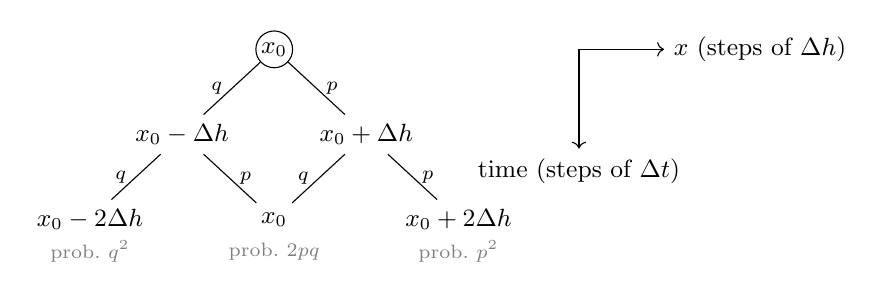
\begin{tikzpicture}[scale=0.9,every node/.style={font=\small}]
\node[draw,circle,inner sep=1pt] (a) at (0,0) {$x_0$};
\node (b1) at (-1.3,-1.2) {$x_0-\Delta h$}; \node (b2) at (1.3,-1.2) {$x_0+\Delta h$};
\node (c1) at (-2.6,-2.4) {$x_0-2\Delta h$}; \node (c2) at (0,-2.4) {$x_0$}; \node (c3) at (2.6,-2.4) {$x_0+2\Delta h$};
\draw (a)--node[left,font=\scriptsize]{$q$}(b1); \draw (a)--node[right,font=\scriptsize]{$p$}(b2);
\draw (b1)--node[left,font=\scriptsize]{$q$}(c1); \draw (b1)--node[right,font=\scriptsize]{$p$}(c2);
\draw (b2)--node[left,font=\scriptsize]{$q$}(c2); \draw (b2)--node[right,font=\scriptsize]{$p$}(c3);
\node[gray,font=\scriptsize] at (-2.6,-2.85) {prob.\ $q^2$};
\node[gray,font=\scriptsize] at (0,-2.85) {prob.\ $2pq$};
\node[gray,font=\scriptsize] at (2.6,-2.85) {prob.\ $p^2$};
\draw[->] (4.3,0)--(5.5,0) node[right]{$x$ (steps of $\Delta h$)};
\draw[->] (4.3,0)--(4.3,-1.4) node[below]{time (steps of $\Delta t$)};
\end{tikzpicture}
\end{center}
\textit{How to read the figure.} Time runs downward, one row per step $\Delta t$; the horizontal position is the value of $x$. From each node the process goes right (up by $\Delta h$) with probability $p$ or left (down by $\Delta h$) with probability $q$. The tree recombines (up-then-down and down-then-up both return to $x_0$), so after two steps the probabilities of the three possible values are $q^2$, $2pq$, $p^2$.

\paragraph{Moments of one step.}
\begin{align*}
\mathbb{E}[\Delta x]&=p\,\Delta h+q\,(-\Delta h)=(p-q)\,\Delta h,\\
\mathbb{E}[(\Delta x)^2]&=p\,(\Delta h)^2+q\,(\Delta h)^2=(\Delta h)^2.
\end{align*}
\paragraph{Choosing the step size.} Set $p=q=\tfrac12$ (no drift, property 1) and $\Delta h=\sigma\sqrt{\Delta t}$, so that $(\Delta h)^2/\Delta t=\sigma^2$. Over a horizon $T$ there are $n=T/\Delta t$ independent steps, so
\[
\operatorname{Var}(x_T-x_0)=n\,(\Delta h)^2=\frac{T}{\Delta t}\,\sigma^2\Delta t=\sigma^2T\qquad(=T\text{ when }\sigma=1),
\]
which is property 2. As $\Delta t\to0$, $x_T-x_0$ is a sum of many iid steps, so by the central limit theorem it becomes Gaussian (property 3).

\begin{tipbox}
The step must scale with $\sqrt{\Delta t}$, not $\Delta t$. If $\Delta h\propto\Delta t$, the variance $\frac{T}{\Delta t}(\Delta h)^2\propto T\Delta t\to0$ and the limit is deterministic; if $\Delta h$ shrinks more slowly than $\sqrt{\Delta t}$ the variance explodes. Only $\Delta h=\sigma\sqrt{\Delta t}$ gives a finite, non-zero variance per unit of time.
\end{tipbox}

%=====================================================================
\subsection{Brownian motion and diffusions \pg{14--16}}

\subsubsection{Standard Brownian motion (SBM)}\label{sec:sbm}
The limit of the binomial tree with $\sigma=1$ is the \emph{standard Brownian motion} $W_t$ (also called a Wiener process). It is a continuous-time Markov process with the following features:
\begin{enumerate}
\item \textbf{Continuous sample paths} (no jumps).
\item \textbf{Nowhere differentiable:} over a step, $\dfrac{\Delta x}{\Delta t}\sim\dfrac{\Delta h}{\Delta t}=\dfrac{\sigma\sqrt{\Delta t}}{\Delta t}=\dfrac{\sigma}{\sqrt{\Delta t}}\to\infty$ as $\Delta t\to0$. Hence $dW/dt$ does not exist; we always work with the increment $dW$ instead.
\item \textbf{Stationary, independent increments:} increments over non-overlapping intervals are independent, and their distribution depends only on the length of the interval.
\item \textbf{Mean zero, variance equal to elapsed time:} $W(0)=0$, $W(t)\sim N(0,t)$, and $W(t)-W(s)\sim N(0,t-s)$ for $s<t$.
\end{enumerate}

\paragraph{Increments.} For any discrete interval $\Delta t$,
\[
\Delta W_t=\varepsilon_t\sqrt{\Delta t},\qquad \varepsilon_t\sim N(0,1)\ \text{iid}.
\]
As $\Delta t\to0$, $dW=\varepsilon\sqrt{dt}$, and
\begin{align*}
\mathbb{E}[dW]&=\mathbb{E}[\varepsilon]\sqrt{dt}=0,\\
\mathbb{E}[(dW)^2]&=\mathbb{E}[\varepsilon^2]\,dt=dt\qquad(\text{since }\mathbb{E}[\varepsilon^2]=\operatorname{Var}\varepsilon=1).
\end{align*}
So $dW\sim N(0,dt)$, and summing increments, $W_t-W_s\sim N(0,t-s)$. Moreover $(dW)^2$ is of order $dt$ (not $dt^2$), which is why second-order terms survive in It\^o's lemma; in the limit one treats $(dW)^2=dt$ as non-random.

\paragraph{$p$-th variation.} For a partition $0=t_0<t_1<\dots<t_n=T$,
\[
V^p=\lim_{\max_k\Delta t_k\to0}\ \sum_{k=1}^n\big|x_{t_k}-x_{t_{k-1}}\big|^p.
\]
For SBM on $[0,T]$: each increment has size of order $\sqrt{\Delta t}$ and there are $T/\Delta t$ of them, so the sum is of order $\frac{T}{\Delta t}(\Delta t)^{p/2}$:
\begin{itemize}
\item $p=1$: order $T/\sqrt{\Delta t}\to\infty$, so $V^1=\infty$ (paths have infinite length; another sign of non-differentiability);
\item $p=2$: order $T$, and in fact $V^2=T$ exactly (\emph{quadratic variation} = elapsed time; this is the integrated form of $(dW)^2=dt$);
\item $p>2$: order $T(\Delta t)^{p/2-1}\to0$, so $V^p=0$.
\end{itemize}

\subsubsection{General (arithmetic) Brownian motion and diffusions}\label{sec:diffusions}
\begin{itemize}
\item \textbf{General (arithmetic) BM.} Build it from SBM by adding a drift $\mu$ and a volatility $\sigma$ (both constants):
\[
x_t=x_0+\mu t+\sigma W_t\qquad\Longleftrightarrow\qquad dx_t=\mu\,dt+\sigma\,dW_t.
\]
The second form is a \emph{stochastic differential equation} (SDE). Then $x_t-x_s\sim N\big(\mu(t-s),\ \sigma^2(t-s)\big)$.
\item \textbf{General diffusion.} Let drift and volatility depend on the state and time:
\[
dx_t=\underbrace{\mu(x,t)\,dt}_{\text{drift}}+\underbrace{\sigma(x,t)\,dW_t}_{\text{diffusion (random fluctuation)}}.
\]
By choosing $\mu(\cdot)$ and $\sigma(\cdot)$ one can generate almost any continuous-time stochastic process with continuous paths. Two important special cases follow.
\end{itemize}

\paragraph{Ornstein--Uhlenbeck (OU) process.} $\mu(x)=\kappa(\bar x-x)$ with $\kappa>0$, $\sigma(x,t)=\sigma$:
\begin{equation}\label{eq:ou}
dx_t=\kappa(\bar x-x_t)\,dt+\sigma\,dW_t.
\end{equation}
\begin{itemize}
\item $\bar x$: long-run mean; $\kappa$: speed of mean reversion (how fast $x$ is pulled back to $\bar x$).
\item When $x>\bar x$ the drift is negative, and when $x<\bar x$ it is positive, so $x$ is always pushed toward $\bar x$.
\item Taking expectations of \eqref{eq:ou} ($\mathbb{E}\,dW=0$): $\frac{d}{dt}\mathbb{E}[x_t]=\kappa(\bar x-\mathbb{E}[x_t])$, so $\mathbb{E}[x_t]=\bar x+(x_0-\bar x)e^{-\kappa t}$: the gap to the mean decays at rate $\kappa$.
\item It is the continuous-time analogue of an AR(1): discretising with step $\Delta t$, $x_{t+\Delta t}\approx(1-\kappa\Delta t)\,x_t+\kappa\Delta t\,\bar x+\sigma\sqrt{\Delta t}\,\varepsilon$, an AR(1) with persistence $\phi=1-\kappa\Delta t\approx e^{-\kappa\Delta t}$.
\item Its stationary distribution is $N(\bar x,\sigma^2/(2\kappa))$ (derived from the KFE above).
\end{itemize}

\begin{center}
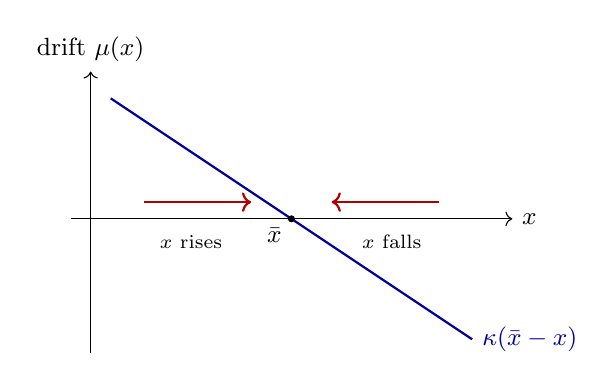
\begin{tikzpicture}[scale=0.85,every node/.style={font=\small}]
\draw[->] (-0.3,0)--(6.3,0) node[right]{$x$};
\draw[->] (0,-2)--(0,2.2) node[above]{drift $\mu(x)$};
\draw[thick,blue!60!black] (0.3,1.8)--(5.7,-1.8) node[right]{$\kappa(\bar x-x)$};
\fill (3,0) circle (1.5pt) node[below left]{$\bar x$};
\draw[->,thick,red!70!black] (0.8,0.25)--(2.4,0.25);
\draw[->,thick,red!70!black] (5.2,0.25)--(3.6,0.25);
\node[font=\scriptsize] at (1.5,-0.35) {$x$ rises};
\node[font=\scriptsize] at (4.5,-0.35) {$x$ falls};
\end{tikzpicture}
\end{center}
\textit{How to read the figure.} The horizontal axis is the current value of $x$; the vertical axis is the drift (expected change per unit of time). The drift line slopes down with slope $-\kappa$ and crosses zero at $\bar x$. To the left of $\bar x$ the drift is positive, so $x$ tends to rise; to the right it is negative, so $x$ tends to fall (red arrows). A steeper line (larger $\kappa$) means faster mean reversion.

\paragraph{Geometric Brownian motion (GBM).} $\mu(x,t)=\mu x$, $\sigma(x,t)=\sigma x$:
\begin{equation}\label{eq:gbm}
dx_t=\mu x_t\,dt+\sigma x_t\,dW_t\qquad\Longleftrightarrow\qquad \frac{dx_t}{x_t}=\mu\,dt+\sigma\,dW_t.
\end{equation}
\begin{itemize}
\item $\mu$ is the expected growth rate of $x$ and $\sigma$ the volatility of its growth rate.
\item The variance of $dx$ is not constant: it is $\sigma^2x^2dt$, proportional to the level of $x$ squared.
\item $x_t>0$ for all $t$ if $x_0>0$. Using It\^o's lemma (Example 2 below), $x_t=x_0\exp\!\big((\mu-\tfrac12\sigma^2)t+\sigma W_t\big)$, so $\log x_t$ is an arithmetic BM and $x_t$ is log-normal with $\mathbb{E}[x_t]=x_0e^{\mu t}$.
\end{itemize}

\subsubsection{Standard vs.\ general BM; BM vs.\ GBM}
\begin{itemize}
\item \textbf{Standard BM:} $W_0=0$ and independent increments $W_{t_2}-W_{t_1}\sim N(0,t_2-t_1)$; in discrete steps $W_t=W_{t-\Delta t}+\varepsilon\sqrt{\Delta t}$, so it is centred at 0.
\item \textbf{General (arithmetic) BM:} has a drift, so it is not centred at 0 (its mean is $x_0+\mu t$). With constant $\mu,\sigma$ its increments are still stationary and independent: $x_t-x_s\sim N\big(\mu(t-s),\sigma^2(t-s)\big)$; and the underlying shock is still $dW_t\sim N(0,dt)$.
\item \textbf{BM = additive shocks:} the size of a shock does not depend on the level of $x$ (e.g.\ labour income).
\item \textbf{GBM = multiplicative shocks:} shocks are proportional to the level of $x$ (e.g.\ investment / capital income: a return shock hits each unit of wealth). This is why capital in the stochastic AK model follows a GBM.
\end{itemize}

%=====================================================================
\subsection{It\^o's lemma \pg{16--17}}\label{sec:ito}

\paragraph{Setup.} $x_t$ follows the diffusion $dx_t=\mu(x,t)\,dt+\sigma(x,t)\,dW_t$, which in integral form reads
\[
x_t=x_0+\int_0^t\mu(x_s,s)\,ds+\int_0^t\sigma(x_s,s)\,dW_s,
\]
where the last term is an It\^o integral. Let $y=f(x,t)$ be a smooth function. Question: given the SDE for $x$, what is the SDE for $y$?

\paragraph{Derivation.} Take a second-order Taylor expansion of $f$:
\[
dy=f_x\,dx+f_t\,dt+\tfrac12f_{xx}(dx)^2+f_{xt}\,dx\,dt+\tfrac12f_{tt}(dt)^2+\dots
\]
In ordinary calculus only first-order terms survive. Here, because $dW=\varepsilon\sqrt{dt}$, the term $(dx)^2$ contains $(dW)^2$, which is of order $dt$ and must be kept. Use the multiplication rules
\[
(dt)^2=0,\qquad dt\cdot dW=0,\qquad (dW)^2=dt
\]
(the first two are of order $dt^{3/2}$ or $dt^2$, negligible relative to $dt$). Then
\begin{align*}
(dx)^2&=\mu^2(dt)^2+2\mu\sigma\,dt\,dW+\sigma^2(dW)^2\qquad\text{(expand the square)}\\
&=0+0+\sigma^2dt=\sigma^2dt,
\end{align*}
and $dx\,dt=0$, $(dt)^2=0$.

\begin{keybox}[title=It\^o's lemma]
\[
dy=\frac{\partial y}{\partial x}dx+\frac{\partial y}{\partial t}dt+\frac12\frac{\partial^2y}{\partial x^2}(dx)^2,
\]
and after substituting $dx$ and $(dx)^2=\sigma^2dt$:
\begin{equation}\label{eq:ito}
dy=\Big(\mu f_x+f_t+\tfrac12\sigma^2f_{xx}\Big)dt+\sigma f_x\,dW.
\end{equation}
Two variables $g(x,y)$:
\[
dg=g_x\,dx+g_y\,dy+\tfrac12g_{xx}(dx)^2+\tfrac12g_{yy}(dy)^2+g_{xy}\,dx\,dy.
\]
\end{keybox}
\textit{Interpretation.} Compared with the ordinary chain rule, the drift of $y$ has an extra term $\tfrac12\sigma^2f_{xx}$: if $f$ is convex, volatility raises the expected change of $y$; if concave, it lowers it (Jensen's inequality).

\begin{tipbox}
Shortcut: when computing $(dx)^2$, square only the $dW$ term; everything with $dt$ drops out.
\end{tipbox}

\paragraph{Example 1: $y=e^x$ with $dx=\mu\,dt+\sigma\,dW$ (arithmetic BM).}
Derivatives: $\dfrac{\partial y}{\partial x}=e^x$, $\dfrac{\partial y}{\partial t}=0$, $\dfrac{\partial^2y}{\partial x^2}=e^x$; and $(dx)^2=\sigma^2dt$.
\begin{align*}
dy&=e^x\,dx+0\cdot dt+\tfrac12e^x(dx)^2\qquad\text{(It\^o's lemma)}\\
&=e^x(\mu\,dt+\sigma\,dW)+\tfrac12e^x\sigma^2dt\qquad\text{(substitute $dx$ and $(dx)^2$)}\\
&=e^x\mu\,dt+e^x\sigma\,dW+\tfrac12e^x\sigma^2dt\\
&=\Big(e^x\mu+\tfrac12\sigma^2e^x\Big)dt+e^x\sigma\,dW\qquad\text{(collect $dt$ terms)}\\
&=\Big(\mu+\tfrac12\sigma^2\Big)y\,dt+\sigma y\,dW\qquad\text{(use $e^x=y$)}.
\end{align*}
So $y=e^x$ is a GBM with growth rate $\mu+\tfrac12\sigma^2>\mu$: because $e^x$ is convex, the volatility of $x$ raises the expected growth of $y$.

\paragraph{Example 2: $y=\log x$.} Derivatives: $y_x=1/x$, $y_{xx}=-1/x^2$, $y_t=0$. Intuitively, since $\log$ is concave, $y$ grows more slowly than the naive guess.

\emph{(a) With $dx=\mu\,dt+\sigma\,dW$ (arithmetic BM):} $(dx)^2=\sigma^2dt$, so
\begin{align*}
dy&=\frac1x(\mu\,dt+\sigma\,dW)-\frac12\frac{1}{x^2}\sigma^2dt\\
&=\Big(\frac{\mu}{x}-\frac{\sigma^2}{2x^2}\Big)dt+\frac{\sigma}{x}\,dW.
\end{align*}
\emph{(b) With GBM $dx=\mu x\,dt+\sigma x\,dW$ (the usual case):} now $(dx)^2=\sigma^2x^2dt$, so
\begin{align*}
dy&=\frac1x(\mu x\,dt+\sigma x\,dW)-\frac12\frac{1}{x^2}\sigma^2x^2dt\\
&=\mu\,dt+\sigma\,dW-\tfrac12\sigma^2dt\\
&=\Big(\mu-\tfrac12\sigma^2\Big)dt+\sigma\,dW.
\end{align*}
\begin{keybox}[title=Log of a GBM]
$d\log x_t=\big(\mu-\tfrac12\sigma^2\big)dt+\sigma\,dW_t$, an arithmetic BM. Integrating from $0$ to $t$: $\log x_t=\log x_0+(\mu-\tfrac12\sigma^2)t+\sigma W_t$, i.e.\ $x_t=x_0\exp\!\big((\mu-\tfrac12\sigma^2)t+\sigma W_t\big)$.
\end{keybox}
The mean growth rate of $x$ is $\mu$, but the growth rate of $\log x$ (the median/typical path) is lower by $\tfrac12\sigma^2$.

\paragraph{Example 3: product of two correlated GBMs.}
\textit{Setup.}
\[
dx=\mu_1x\,dt+\sigma_1x\,dW_1,\qquad dy=\mu_2y\,dt+\sigma_2y\,dW_2,\qquad dW_2=\rho\,dW_1+\sqrt{1-\rho^2}\,dZ,
\]
where $W_1$ and $Z$ are two uncorrelated SBMs and $\rho\in[-1,1]$ is the correlation between $dW_1$ and $dW_2$ (here $\rho$ is a correlation, not the discount rate). Find $dg$ for $g=xy$.

\textit{Step 1: derivatives.} $g_x=y$, $g_y=x$, $g_{xx}=0$, $g_{yy}=0$, $g_{xy}=1$.

\textit{Step 2: the cross term.} Using $(dW_1)^2=dt$ and $dW_1\,dZ=0$ (uncorrelated), and dropping all products involving $dt$:
\begin{align*}
dx\,dy&=\sigma_1\sigma_2\,xy\,dW_1\,dW_2\\
&=\sigma_1\sigma_2\,xy\,dW_1\big(\rho\,dW_1+\sqrt{1-\rho^2}\,dZ\big)\\
&=\sigma_1\sigma_2\,xy\,\big(\rho\,dt+0\big)=\rho\,\sigma_1\sigma_2\,g\,dt.
\end{align*}
\textit{Step 3: apply the two-variable It\^o formula.}
\begin{align*}
dg&=y\,dx+x\,dy+\tfrac12\cdot0\cdot(dx)^2+\tfrac12\cdot0\cdot(dy)^2+1\cdot dx\,dy\\
&=y(\mu_1x\,dt+\sigma_1x\,dW_1)+x(\mu_2y\,dt+\sigma_2y\,dW_2)+\rho\sigma_1\sigma_2\,xy\,dt\\
&=(\mu_1+\mu_2+\rho\sigma_1\sigma_2)\,g\,dt+\sigma_1g\,dW_1+\sigma_2g\,dW_2.
\end{align*}
\textit{Step 4: volatility of $g$.} The shock term $\sigma_1\,dW_1+\sigma_2\,dW_2$ has variance per unit of time
$\sigma_1^2+\sigma_2^2+2\rho\sigma_1\sigma_2$ (variance of a sum with covariance $\rho\sigma_1\sigma_2$).

\begin{keybox}[title=Takeaways]
The product of two GBMs is again a GBM, with
\[
\frac{dg}{g}=(\mu_1+\mu_2+\rho\sigma_1\sigma_2)\,dt+\sigma_g\,d\widetilde W,\qquad \sigma_g=\sqrt{\sigma_1^2+\sigma_2^2+2\rho\sigma_1\sigma_2},
\]
where $\widetilde W$ is an SBM. Similarly, the sum of arithmetic (additive) BMs is again an arithmetic BM.
\end{keybox}
\textit{Interpretation.} The drift of the product is not just $\mu_1+\mu_2$: positive correlation ($\rho>0$) adds $\rho\sigma_1\sigma_2$, because when $x$ is high $y$ also tends to be high. Check via logs: $d\log g=d\log x+d\log y$ has drift $\mu_1+\mu_2-\tfrac12(\sigma_1^2+\sigma_2^2)$, which equals $\mu_g-\tfrac12\sigma_g^2$ with $\mu_g=\mu_1+\mu_2+\rho\sigma_1\sigma_2$, as it must.

%=====================================================================
\subsection{Markov chains: transition matrix and stationary distribution \pg{70}}

\paragraph{Setup (HW Q3).}
\begin{itemize}
\item $\lambda_t$: gross growth rate of the economy; it takes two values: bad state $\lambda_1=0.98$ (output shrinks 2\%), good state $\lambda_2=1.03$ (output grows 3\%).
\item $\lambda_t$ follows a (first-order) \emph{Markov chain}: the probability distribution of $\lambda_{t+1}$ depends only on the current state $\lambda_t$, not on earlier history.
\item $p_{ij}=\Pr(\lambda_{t+1}=\lambda_j\mid\lambda_t=\lambda_i)$: transition probabilities, collected in the \emph{transition matrix} $P$ (rows = today's state, columns = tomorrow's state; each row sums to 1).
\item $\pi_i$: long-run (stationary) probability of being in state $i$.
\end{itemize}
\[
P=\begin{bmatrix}p_{11}&1-p_{11}\\1-p_{22}&p_{22}\end{bmatrix}=\begin{bmatrix}0.8&0.2\\0.15&0.85\end{bmatrix}.
\]

\begin{center}
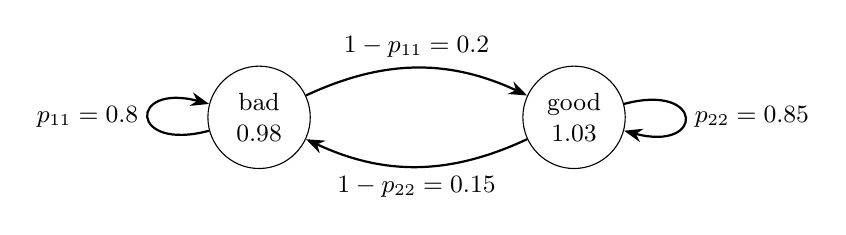
\begin{tikzpicture}[every node/.style={font=\small},>=Stealth]
\node[draw,circle,minimum size=1.3cm,align=center] (s1) at (0,0) {bad\\$0.98$};
\node[draw,circle,minimum size=1.3cm,align=center] (s2) at (4,0) {good\\$1.03$};
\draw[->,thick] (s1) to[bend left=25] node[above]{$1-p_{11}=0.2$} (s2);
\draw[->,thick] (s2) to[bend left=25] node[below]{$1-p_{22}=0.15$} (s1);
\draw[->,thick] (s1) to[loop left] node[left]{$p_{11}=0.8$} (s1);
\draw[->,thick] (s2) to[loop right] node[right]{$p_{22}=0.85$} (s2);
\end{tikzpicture}
\end{center}
\textit{How to read the figure.} Each circle is a state. An arrow from state $i$ to state $j$ carries the probability of moving from $i$ today to $j$ tomorrow; self-loops are the probabilities of staying. The probabilities on the arrows leaving any state sum to 1 (one row of $P$).

\paragraph{Reading the matrix.}
\begin{itemize}
\item If today we are in state 1 ($\lambda_t=0.98$): stay in state 1 with probability $p_{11}=0.8$; move to state 2 ($\lambda_{t+1}=1.03$) with probability $0.2$.
\item If today we are in state 2 ($\lambda_t=1.03$): stay in state 2 with probability $p_{22}=0.85$; move to state 1 ($\lambda_{t+1}=0.98$) with probability $0.15$.
\end{itemize}
Conditional expectations of next period's growth:
\begin{align*}
\mathbb{E}[\lambda_{t+1}\mid\lambda_t=0.98]&=0.8(0.98)+0.2(1.03)=0.784+0.206=0.990,\\
\mathbb{E}[\lambda_{t+1}\mid\lambda_t=1.03]&=0.15(0.98)+0.85(1.03)=0.147+0.8755=1.0225.
\end{align*}
Expected duration of a spell in state $i$ is $1/(1-p_{ii})$: $1/0.2=5$ periods for the bad state, $1/0.15\approx6.67$ periods for the good state.

\paragraph{Stationary distribution.} The goal is the unconditional mean $\mathbb{E}[\lambda]=\pi_1\lambda_1+\pi_2\lambda_2$, which requires the long-run probabilities $\pi=(\pi_1,\pi_2)$ (a row vector). Stationarity means that if today's state distribution is $\pi$, tomorrow's is also $\pi$:
\[
\pi=\pi P,\qquad \pi_1+\pi_2=1.
\]
Written out (probability of being in state $j$ tomorrow = sum over today's states of ``probability of being there'' times ``probability of moving to $j$''):
\begin{align}
\pi_1&=\pi_1p_{11}+\pi_2(1-p_{22}),\label{eq:mc1}\\
\pi_2&=\pi_1(1-p_{11})+\pi_2p_{22}.\label{eq:mc2}
\end{align}
Equations \eqref{eq:mc1} and \eqref{eq:mc2} are the same condition (adding them gives $\pi_1+\pi_2=\pi_1+\pi_2$), so we use one of them together with the adding-up constraint.

\textit{Step 1: rearrange \eqref{eq:mc1}.}
\begin{align*}
\pi_1-\pi_1p_{11}&=\pi_2(1-p_{22})\qquad\text{(move $\pi_1p_{11}$ to the left)}\\
\pi_1(1-p_{11})&=\pi_2(1-p_{22})\qquad\text{(flow out of state 1 = flow into state 1)}\\
\pi_2&=\frac{1-p_{11}}{1-p_{22}}\,\pi_1.
\end{align*}
\textit{Step 2: use $\pi_1+\pi_2=1$.}
\begin{align*}
\pi_1\Big(1+\frac{1-p_{11}}{1-p_{22}}\Big)&=1\\
\pi_1\,\frac{(1-p_{22})+(1-p_{11})}{1-p_{22}}&=1\\
\pi_1&=\frac{1-p_{22}}{2-p_{11}-p_{22}},\qquad \pi_2=1-\pi_1=\frac{1-p_{11}}{2-p_{11}-p_{22}}.
\end{align*}
\textit{Step 3: plug in the numbers.} $2-p_{11}-p_{22}=2-0.8-0.85=0.35$, so
\[
\pi_1=\frac{0.15}{0.35}=\frac37\approx0.4286,\qquad \pi_2=\frac{0.2}{0.35}=\frac47\approx0.5714.
\]
\textit{Check:} first column of $\pi P$: $\tfrac37(0.8)+\tfrac47(0.15)=\tfrac{2.4+0.6}{7}=\tfrac37=\pi_1$. \checkmark

\textit{Step 4: unconditional mean growth.}
\[
\mathbb{E}[\lambda]=\pi_1\lambda_1+\pi_2\lambda_2=\frac37(0.98)+\frac47(1.03)=\frac{2.94+4.12}{7}=\frac{7.06}{7}\approx1.0086.
\]

\begin{keybox}[title=Two-state Markov chain]
\[
\pi_1=\frac{1-p_{22}}{2-p_{11}-p_{22}},\qquad \pi_2=\frac{1-p_{11}}{2-p_{11}-p_{22}}.
\]
In HW Q3: $\pi=(3/7,\,4/7)$ and $\mathbb{E}[\lambda]\approx1.0086$, i.e.\ average growth of about $0.86\%$ per period.
\end{keybox}
\textit{Interpretation.} In the long run the economy spends more time in the good state because the good state is more persistent ($p_{22}=0.85>p_{11}=0.8$): the probability of leaving it is smaller. Each $\pi_i$ is proportional to the probability of \emph{leaving the other state}. Starting from any initial state, the rows of $P^n$ converge to $\pi$ as $n\to\infty$; the speed of convergence is governed by the second eigenvalue of $P$, $p_{11}+p_{22}-1=0.65$ (which is also the first-order autocorrelation of $\lambda_t$).

\section{Asset Pricing: Lucas Tree and Complete Markets}

This section has two parts. Part one is the Lucas (1978) tree model: a single representative household prices a risky asset (a ``tree''), and we derive the consumption-based asset-pricing formula. Part two is the complete-markets (Arrow--Debreu) economy with many households: we derive the equilibrium allocation, show that it coincides with a planner's solution, and use Arrow--Debreu prices to price any asset.

%======================================================================
\subsection{Lucas tree model: setup \pg{18}}

\paragraph{Setup.}
\begin{itemize}
  \item \textbf{Time} is discrete, $t=0,1,2,\dots$; agents live forever and discount the future with factor $\beta\in(0,1)$.
  \item \textbf{Assets.} The only assets are identical, infinitely lived \emph{trees}. Each tree yields $d_t$ units of fruit in period $t$. $d_t$ is random and exogenous (the ``dividend''). Fruit is \emph{nondurable}: it must be eaten in the period it appears or it rots.
  \item \textbf{Endowment economy}: there is no production and no storage. The only goods available are the fruit.
  \item \textbf{Notation.}
  \begin{itemize}
    \item $C_t$: consumption of fruit per person; $L_t$: population.
    \item $k_t$: number of trees (shares) per person; $k^i_t$: trees held by household $i$ at the \emph{start} of period $t$.
    \item $p_t$: equilibrium price of one tree, in units of fruit. It is an \emph{ex-dividend} price: if a tree is sold in period $t$, the sale happens \emph{after} the current owner has collected the fruit $d_t$.
    \item $u(\cdot)$: period utility, with $u'>0$, $u''<0$.
    \item $E_t[\cdot]$: expectation conditional on all information available at date $t$ (in particular $d_t$ and $p_t$ are known at $t$).
  \end{itemize}
  \item \textbf{Resource constraint}: aggregate consumption equals aggregate fruit,
  \begin{equation}\label{eq:s4_rc}
    C_tL_t = d_t k_t L_t \quad\Longleftrightarrow\quad C_t = d_t k_t .
  \end{equation}
  Normalizing the supply of trees to one per person ($k_t=1$) gives $C_t=d_t$.
\end{itemize}

\paragraph{Household budget constraint.}
In period $t$ household $i$ arrives with $k^i_t$ trees. Its income is the fruit from those trees plus the value of the trees if sold. It spends on consumption and on the trees it carries into $t+1$:
\begin{equation}\label{eq:s4_bc}
  \underbrace{p_t k^i_{t+1} + C^i_t}_{\text{spending: new trees + consumption}}
  \;=\;
  \underbrace{(d_t + p_t)\,k^i_t}_{\text{income: dividends + value of trees}} .
\end{equation}
Solve \eqref{eq:s4_bc} for next period's holdings. Subtract $C^i_t$ and divide by $p_t$:
\begin{align}
  k^i_{t+1} &= \frac{(d_t+p_t)k^i_t - C^i_t}{p_t} \notag\\
            &= \Big(1+\frac{d_t}{p_t}\Big)k^i_t - \frac{C^i_t}{p_t}. \label{eq:s4_lom_k}
\end{align}

\paragraph{Wealth and return.}
Define wealth at the start of $t$ (value of fruit plus value of trees) and the gross return on a tree from $t$ to $t+1$:
\begin{equation}\label{eq:s4_def_mR}
  m^i_t \equiv (p_t+d_t)\,k^i_t,
  \qquad
  R_{t+1} \equiv \frac{p_{t+1}+d_{t+1}}{p_t}.
\end{equation}
$R_{t+1}$ = (capital gain + dividend) per unit of money invested. Derive the law of motion of wealth:
\begin{align}
  m^i_{t+1} &= (p_{t+1}+d_{t+1})\,k^i_{t+1} && \text{(definition at $t+1$)}\notag\\
  &= (p_{t+1}+d_{t+1})\,\frac{(d_t+p_t)k^i_t - C^i_t}{p_t} && \text{(substitute \eqref{eq:s4_lom_k})}\notag\\
  &= \frac{p_{t+1}+d_{t+1}}{p_t}\,\big(m^i_t - C^i_t\big) && \text{(use $m^i_t=(p_t+d_t)k^i_t$)}\notag\\
  &= R_{t+1}\,\big(m^i_t - C^i_t\big). && \text{(definition of $R_{t+1}$)} \label{eq:s4_lom_m}
\end{align}
Interpretation: whatever wealth is not eaten is invested in trees and earns the random gross return $R_{t+1}$.

\paragraph{Household problem.}
The household chooses a consumption plan to maximize expected discounted utility from date $t$ onward (expectations are taken at $t$, not at $0$):
\begin{equation}\label{eq:s4_seq}
  V(m^i_t) = \max_{\{C^i_{t+n}\}_{n\ge0}} E_t\sum_{n=0}^{\infty}\beta^n u(C^i_{t+n})
  \quad\text{s.t. \eqref{eq:s4_lom_m} in every period.}
\end{equation}
The value function $V$ depends on current wealth $m^i_t$ (it also depends on the current state of the dividend process, which we suppress). The recursive (Bellman) form is
\begin{equation}\label{eq:s4_bellman}
  V(m^i_t) = \max_{C^i_t}\Big\{u(C^i_t) + \beta E_t\big[V(m^i_{t+1})\big]\Big\},
  \qquad m^i_{t+1} = R_{t+1}(m^i_t - C^i_t).
\end{equation}
We substitute the law of motion for $m^i_{t+1}$ directly into the objective, so there is no separate constraint or multiplier.

%======================================================================
\subsection{Euler equation and the stochastic discount factor \pg{18--19}}

\paragraph{Step 1: first-order condition.}
Differentiate the right-hand side of \eqref{eq:s4_bellman} with respect to $C^i_t$ (chain rule: $\frac{d}{dC}V(m(C)) = V'(m)\,\frac{\partial m}{\partial C}$):
\begin{align*}
  0 &= u'(C^i_t) + \beta E_t\Big[V'(m^i_{t+1})\,\frac{\partial m^i_{t+1}}{\partial C^i_t}\Big].
\end{align*}
From \eqref{eq:s4_lom_m}, $\partial m^i_{t+1}/\partial C^i_t = -R_{t+1}$. Substitute and move the expectation term to the left:
\begin{equation}\label{eq:s4_foc}
  u'(C^i_t) = \beta E_t\big[R_{t+1}\,V'(m^i_{t+1})\big].
\end{equation}
Meaning: eating one more unit today gives $u'(C^i_t)$; investing it instead gives $R_{t+1}$ units of wealth tomorrow, each worth $V'(m^i_{t+1})$, discounted by $\beta$.

\paragraph{Step 2: envelope condition.}
\emph{Envelope theorem}: if $V(\theta)=\max_x f(x,\theta)$ with maximizer $x^*(\theta)$, then $V'(\theta) = \partial f(x^*,\theta)/\partial\theta$ (the indirect effect through $x^*$ is zero because $\partial f/\partial x=0$ at the optimum).
Apply it to \eqref{eq:s4_bellman} with $\theta = m^i_t$. Since $\partial m^i_{t+1}/\partial m^i_t = R_{t+1}$,
\begin{align*}
  V'(m^i_t) &= \beta E_t\big[R_{t+1}\,V'(m^i_{t+1})\big] && \text{(envelope theorem)}\\
            &= u'(C^i_t). && \text{(by the FOC \eqref{eq:s4_foc})}
\end{align*}
This holds at every date, so shifting it one period forward:
\begin{equation}\label{eq:s4_env}
  V'(m^i_{t+1}) = u'(C^i_{t+1}).
\end{equation}
The marginal value of wealth equals the marginal utility of consumption.

\paragraph{Step 3: Euler equation.}
Substitute \eqref{eq:s4_env} into \eqref{eq:s4_foc}, then the definition of $R_{t+1}$:
\begin{align*}
  u'(C^i_t) &= \beta E_t\big[R_{t+1}\,u'(C^i_{t+1})\big]\\
  &= \beta E_t\Big[\frac{p_{t+1}+d_{t+1}}{p_t}\,u'(C^i_{t+1})\Big].
\end{align*}
Multiply both sides by $p_t$ and divide by $u'(C^i_t)$ (both are known at $t$, so they can move inside $E_t$):
\begin{equation}\label{eq:s4_euler_i}
  p_t = \beta E_t\!\left[\frac{u'(C^i_{t+1})}{u'(C^i_t)}\,(p_{t+1}+d_{t+1})\right].
\end{equation}
This is the asset-pricing Euler equation, a \emph{first-order stochastic difference equation} in $p_t$. Interpretation: at the optimum the cost of a tree today ($p_t$, in fruit) equals the expected value of what it pays tomorrow (price + dividend), converted into today's fruit using the marginal rate of substitution $\beta u'(C_{t+1})/u'(C_t)$.

\paragraph{Step 4: equilibrium.}
All households are identical (representative agent), and fruit cannot be stored. So in equilibrium everybody holds one tree and eats its fruit: $C^i_t = C_t = d_t$ (from \eqref{eq:s4_rc} with $k_t=1$). The only source of goods is $d$, and what comes in must be eaten. Substituting $C_t=d_t$ into \eqref{eq:s4_euler_i}:

\begin{keybox}[title=Lucas asset-pricing formula]
\begin{equation}\label{eq:s4_lucas}
  p_t = \beta E_t\!\left[\frac{u'(d_{t+1})}{u'(d_t)}\,(p_{t+1}+d_{t+1})\right]
  \quad\Longleftrightarrow\quad
  p_t = E_t\big[M_{t,t+1}\,(p_{t+1}+d_{t+1})\big],
\end{equation}
where the \textbf{stochastic discount factor (SDF)} between $t$ and $t+n$ is
\begin{equation}\label{eq:s4_sdf}
  M_{t,t+n} \equiv \beta^n\,\frac{u'(d_{t+n})}{u'(d_t)} .
\end{equation}
Dividing \eqref{eq:s4_lucas} by $p_t$ gives the equivalent form $1 = E_t\big[M_{t,t+1}R_{t+1}\big]$.
\end{keybox}
The SDF is ``stochastic'' because $d_{t+n}$ is random: a unit of fruit at $t+n$ is worth more today if it arrives in a state where fruit is scarce ($d_{t+n}$ low, $u'(d_{t+n})$ high). Note $M_{t,t+1}M_{t+1,t+2}=M_{t,t+2}$: the $u'(d_{t+1})$ terms cancel.

\paragraph{Risk-free rate.} A one-period risk-free bond pays $1$ for sure at $t+1$. Applying \eqref{eq:s4_lucas} to its payoff (price $=E_t[M_{t,t+1}\cdot 1]$) gives the gross risk-free rate $1+r_{f,t} = 1/E_t[M_{t,t+1}]$.

%======================================================================
\subsection{Iterating forward: price = present value of dividends \pg{19}}

Equation \eqref{eq:s4_lucas} links $p_t$ to $p_{t+1}$. Iterating it removes future prices.

\emph{Law of iterated expectations}: $E_t\big[E_{t+1}[X]\big]=E_t[X]$.

Write \eqref{eq:s4_lucas} at $t+1$: $p_{t+1}=E_{t+1}[M_{t+1,t+2}(p_{t+2}+d_{t+2})]$. Substitute into \eqref{eq:s4_lucas} at $t$:
\begin{align*}
  p_t &= E_t\big[M_{t,t+1}d_{t+1}\big] + E_t\big[M_{t,t+1}\,p_{t+1}\big]\\
  &= E_t\big[M_{t,t+1}d_{t+1}\big] + E_t\Big[M_{t,t+1}\,E_{t+1}\big[M_{t+1,t+2}(p_{t+2}+d_{t+2})\big]\Big]
     && \text{(substitute $p_{t+1}$)}\\
  &= E_t\big[M_{t,t+1}d_{t+1}\big] + E_t\big[M_{t,t+2}(p_{t+2}+d_{t+2})\big]
     && \text{(iterated exp.; $M_{t,t+1}M_{t+1,t+2}=M_{t,t+2}$)}\\
  &= E_t\big[M_{t,t+1}d_{t+1}+M_{t,t+2}d_{t+2}\big] + E_t\big[M_{t,t+2}\,p_{t+2}\big].
\end{align*}
Repeating $n$ times:
\begin{equation}\label{eq:s4_iter}
  p_t = E_t\sum_{j=1}^{n} M_{t,t+j}\,d_{t+j} \;+\; E_t\big[M_{t,t+n}\,p_{t+n}\big].
\end{equation}
\textbf{No-bubble (transversality) condition}: $\lim_{n\to\infty}E_t[M_{t,t+n}p_{t+n}] = 0$, i.e.\ the discounted value of the asset far in the future vanishes. Imposing it and letting $n\to\infty$:
\begin{keybox}[title=Fundamental value]
\begin{equation}\label{eq:s4_pv}
  p_t = E_t\sum_{j=1}^{\infty} M_{t,t+j}\,d_{t+j}
      = E_t\sum_{j=1}^{\infty} \beta^j\,\frac{u'(d_{t+j})}{u'(d_t)}\,d_{t+j}.
\end{equation}
\end{keybox}
The price of a tree is the expected present value of all its future dividends, where each dividend is discounted with the SDF (time discounting $\beta^j$ times a marginal-utility adjustment for risk).

%======================================================================
\subsection{Special case 1: CRRA and log utility --- the price/dividend ratio \pg{19--20}}

\paragraph{Setup.} CRRA utility $u(c)=\frac{c^{1-\rho}}{1-\rho}$, $\rho>0$ (log utility $u=\ln c$ when $\rho=1$). Then $u'(c)=c^{-\rho}$, and in equilibrium $c=d$, so $u'(d)=d^{-\rho}$.

Substitute into \eqref{eq:s4_lucas}:
\begin{align}
  p_t &= \beta E_t\Big[\frac{d_{t+1}^{-\rho}}{d_t^{-\rho}}(p_{t+1}+d_{t+1})\Big]\notag\\
      &= \beta\, d_t^{\rho}\,E_t\big[d_{t+1}^{-\rho}(p_{t+1}+d_{t+1})\big]. \label{eq:s4_crra}
\end{align}

\paragraph{Log utility ($\rho=1$).}
Set $\rho=1$ in \eqref{eq:s4_crra} and divide both sides by $d_t$:
\begin{align*}
  \frac{p_t}{d_t} &= \beta E_t\Big[\frac{p_{t+1}+d_{t+1}}{d_{t+1}}\Big] && \text{(divide by $d_t$)}\\
  &= \beta\Big(1 + E_t\Big[\frac{p_{t+1}}{d_{t+1}}\Big]\Big). && \text{(split the fraction)}
\end{align*}
This is a difference equation in the price/dividend (P/D) ratio. Apply it again at $t+1$ and use iterated expectations:
\begin{align*}
  \frac{p_t}{d_t} &= \beta\Big(1 + \beta\Big(1 + E_t\Big[\frac{p_{t+2}}{d_{t+2}}\Big]\Big)\Big)
  = \beta + \beta^2 + \beta^2E_t\Big[\frac{p_{t+2}}{d_{t+2}}\Big]\\
  &= \beta + \beta^2 + \dots + \beta^n + \beta^n E_t\Big[\frac{p_{t+n}}{d_{t+n}}\Big]. && \text{(after $n$ steps)}
\end{align*}
Under the no-bubble condition $\lim_{n\to\infty}\beta^nE_t[p_{t+n}/d_{t+n}]=0$, the last term vanishes. The rest is a geometric series ($\sum_{j=1}^\infty \beta^j = \beta/(1-\beta)$ for $|\beta|<1$):
\begin{keybox}[title=Log utility: constant P/D ratio]
\[
  \frac{p_t}{d_t} = \frac{\beta}{1-\beta}\qquad\text{(for every $t$ and every dividend process).}
\]
\end{keybox}
Check with \eqref{eq:s4_pv}: with log utility $M_{t,t+j}d_{t+j} = \beta^j\frac{d_t}{d_{t+j}}d_{t+j}=\beta^jd_t$, which is not random, so $p_t=d_t\sum_{j\ge1}\beta^j = d_t\beta/(1-\beta)$. Same answer.

\paragraph{Interpretation.} The price is proportional to today's dividend and does not depend on expected \emph{future} dividends. Why?
\begin{itemize}
  \item \emph{Substitution (cash-flow) effect}: good news about $d_{t+j}$ raises the tree's future payoff, which raises its price.
  \item \emph{Income (discounting) effect}: higher $d_{t+j}$ also means higher future consumption, so $u'(d_{t+j})$ (the SDF) falls and future fruit is worth less today, which lowers its price.
  \item With log utility the two effects cancel exactly: $u'(d)\cdot d = 1$. This is the same logic as constant expenditure shares under log/Cobb--Douglas preferences.
\end{itemize}

\paragraph{General CRRA with i.i.d.\ growth.}
The constant P/D ratio holds for every dividend process only when $\rho=1$. For $\rho\ne1$, a constant ratio needs extra assumptions. Assume dividend growth $g_{t+1}\equiv d_{t+1}/d_t$ is i.i.d. Guess $p_t = v\,d_t$ for a constant $v$ and substitute into \eqref{eq:s4_crra}:
\begin{align*}
  v\,d_t &= \beta\,d_t^{\rho}\,E_t\big[d_{t+1}^{-\rho}(v+1)d_{t+1}\big]
          = \beta(1+v)\,d_t^{\rho}\,E_t\big[d_{t+1}^{1-\rho}\big]\\
  v &= \beta(1+v)\,E_t\Big[\Big(\frac{d_{t+1}}{d_t}\Big)^{1-\rho}\Big] && \text{(divide by $d_t$)}\\
  v &= \beta(1+v)\,E\big[g^{1-\rho}\big]. && \text{(i.i.d.: the expectation is a constant)}
\end{align*}
Collect the $v$ terms: $v\big(1-\beta E[g^{1-\rho}]\big)=\beta E[g^{1-\rho}]$, so
\[
  \frac{p_t}{d_t} = v = \frac{\beta E[g^{1-\rho}]}{1-\beta E[g^{1-\rho}]},\qquad \text{provided } \beta E[g^{1-\rho}]<1 .
\]
With $\rho=1$, $g^{0}=1$ and we recover $\beta/(1-\beta)$. Comparative statics: higher growth raises $E[g^{1-\rho}]$ (and hence $v$) if $\rho<1$ (substitution effect dominates), and lowers it if $\rho>1$ (income effect dominates).

%======================================================================
\subsection{Special case 2: risk neutrality, martingales and efficient markets \pg{19--20}}

\paragraph{Setup.} Risk neutrality means $u$ is linear, so $u'$ is constant and $u'(d_{t+1})/u'(d_t)=1$. Then $M_{t,t+1}=\beta$ (no adjustment for risk), and from the bond-pricing result $1+r_f = 1/\beta$, i.e.\ $\beta=\frac{1}{1+r_f}$ with $r_f$ the (constant) risk-free rate.

Substitute into \eqref{eq:s4_lucas}:
\begin{align}
  p_t &= \beta E_t\big[p_{t+1}+d_{t+1}\big] = \frac{1}{1+r_f}E_t\big[p_{t+1}+d_{t+1}\big] \notag\\
  \Longleftrightarrow\quad E_t\big[p_{t+1}+d_{t+1}\big] &= \frac{p_t}{\beta} = (1+r_f)\,p_t
  \quad\Longleftrightarrow\quad E_t[R_{t+1}] = 1+r_f . \label{eq:s4_rn}
\end{align}

\paragraph{Martingale.} A process $x_t$ is a \emph{martingale} with respect to information sets $I_t$ if $E[x_{t+1}\mid I_t]=x_t$. A random walk $x_{t+1}=x_t+\varepsilon_{t+1}$ with $E[\varepsilon_{t+1}\mid I_t]=0$ is a special case.

Under risk neutrality the price is a martingale \emph{after adjusting for discounting and dividends}: by \eqref{eq:s4_rn} the expected return is the constant $1+r_f$. For example, if the asset pays no dividends, $E_t[\beta^{t+1}p_{t+1}]=\beta^tp_t$, so the discounted price $\beta^tp_t$ is a martingale. Hence expected returns are constant and \emph{changes in returns cannot be predicted} from current information.

\paragraph{Risk aversion breaks the martingale property.}
Write $1=E_t[M_{t,t+1}R_{t+1}]$ using $E[XY]=E[X]E[Y]+\mathrm{Cov}(X,Y)$:
\begin{align*}
  1 &= E_t[M_{t,t+1}]\,E_t[R_{t+1}] + \mathrm{Cov}_t(M_{t,t+1},R_{t+1})\\
  E_t[R_{t+1}] &= \frac{1-\mathrm{Cov}_t(M_{t,t+1},R_{t+1})}{E_t[M_{t,t+1}]}
  = (1+r_{f,t})\big[1-\mathrm{Cov}_t(M_{t,t+1},R_{t+1})\big].
\end{align*}
With risk aversion $M_{t,t+1}$ varies with $d_{t+1}$, so $r_{f,t}$ and the covariance term can move over time with the state. Expected returns then vary over time, and returns can be predictable even though markets are efficient. An asset whose return is high when $M$ is low (good times) has a negative covariance and must offer a risk premium.

\begin{keybox}[title=Lucas takeaway]
Asset prices are in general \emph{not} a random walk or martingale. ``Martingale $\Leftrightarrow$ efficient markets'' holds only under risk neutrality. With risk-averse agents an efficient market (no arbitrage, prices reflect all available information) can produce predictable returns, because required returns change with marginal utility.
\end{keybox}
The efficient-markets hypothesis (EMH) says prices reflect all available information. Combined with \eqref{eq:s4_rn}, today's price $p_t$ summarizes the market's \emph{expectation} of the discounted future payoff. It does not make the future price known: $p_{t+1}$ is still random.

\paragraph{Comments on the Lucas model.}
\begin{enumerate}
  \item It is a representative-agent model: one consumer whose preferences and endowment stand for the whole economy.
  \item There is no trade in equilibrium (any trade would be between identical agents). Prices adjust until the representative agent is just willing to hold the tree and eat its fruit; the Euler equation \eqref{eq:s4_lucas} gives exactly that price.
\end{enumerate}

%======================================================================
\subsection{Complete markets: the Arrow--Debreu economy \pg{21--22}}

\paragraph{Setup: uncertainty.}
\begin{itemize}
  \item Each period a state $s_t$ is drawn from a finite set $S$. It follows a Markov chain with transition probabilities $\Pr[s_{t+1}=s'\mid s_t=s]=\pi(s'\mid s)$.
  \item The \emph{history} up to $t$ is $s^t\equiv(s_0,s_1,\dots,s_t)$. Given the initial state $s_0$, its probability is the product of one-step transitions (chain rule of probability plus the Markov property):
  \begin{equation}\label{eq:s4_hist}
    \pi(s^t\mid s_0) = \pi(s_t\mid s_{t-1})\,\pi(s_{t-1}\mid s_{t-2})\cdots\pi(s_1\mid s_0).
  \end{equation}
\end{itemize}

\begin{center}
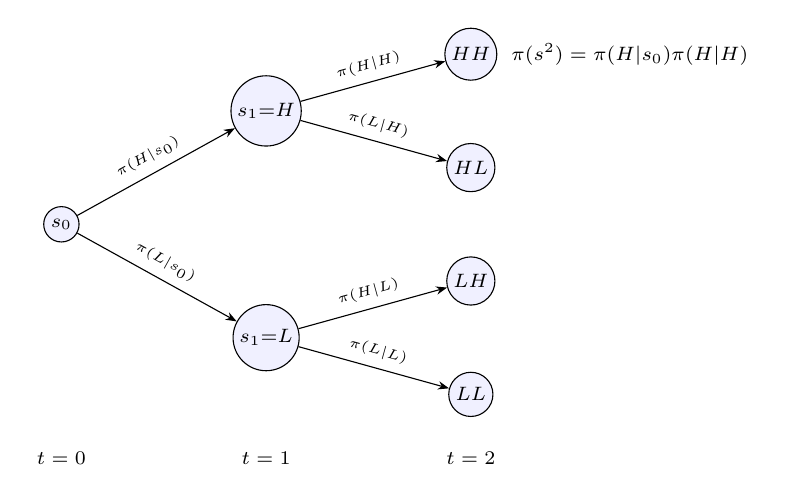
\begin{tikzpicture}[x=2.6cm,y=0.9cm,
  nd/.style={circle,draw,fill=blue!6,inner sep=1.5pt,font=\scriptsize}]
  \node[nd] (r) at (0,0) {$s_0$};
  \node[nd] (a) at (1,1.6) {$s_1{=}H$};
  \node[nd] (b) at (1,-1.6) {$s_1{=}L$};
  \node[nd] (aa) at (2,2.4) {$HH$};
  \node[nd] (ab) at (2,0.8) {$HL$};
  \node[nd] (ba) at (2,-0.8) {$LH$};
  \node[nd] (bb) at (2,-2.4) {$LL$};
  \foreach \u/\v/\l in {r/a/{\pi(H|s_0)},r/b/{\pi(L|s_0)},a/aa/{\pi(H|H)},a/ab/{\pi(L|H)},b/ba/{\pi(H|L)},b/bb/{\pi(L|L)}}
    \draw[-{Stealth[length=4pt]}] (\u) -- node[midway,above,sloped,font=\tiny]{$\l$} (\v);
  \node[font=\scriptsize] at (0,-3.3) {$t=0$};
  \node[font=\scriptsize] at (1,-3.3) {$t=1$};
  \node[font=\scriptsize] at (2,-3.3) {$t=2$};
  \node[font=\scriptsize,anchor=west] at (2.15,2.4) {$\pi(s^2)=\pi(H|s_0)\pi(H|H)$};
\end{tikzpicture}
\end{center}
\emph{How to read the event tree.} Time runs left to right; each node is a history $s^t$ (here with two states, $H$ and $L$). Each branch is labelled with its one-step transition probability, and the probability of reaching a node is the product of the probabilities along its path, as in \eqref{eq:s4_hist}. An Arrow--Debreu security (defined below) is a claim to one unit of goods at exactly one node.

\paragraph{Setup: households.}
\begin{itemize}
  \item $I$ households, $i=1,\dots,I$. Household $i$ has a stochastic endowment $y^i_t(s^t)$ (goods received at $t$ after history $s^t$).
  \item $c^i_t(s^t)$: consumption of $i$ at $t$ after history $s^t$. A consumption plan $c^i$ lists this for all $(t,s^t)$.
  \item Preferences: expected discounted utility. Writing the expectation out as a probability-weighted sum over histories,
  \begin{equation}\label{eq:s4_U}
    U(c^i) = E_0\sum_{t=0}^{\infty}\beta^t u\big(c^i_t\big)
    = \sum_{t=0}^{\infty}\sum_{s^t}\beta^t\,\pi(s^t\mid s_0)\,u\big[c^i_t(s^t)\big].
  \end{equation}
  The sum over $t$ runs over time; the sum over $s^t$ with weights $\pi(s^t\mid s_0)$ runs over all possible histories (this is what $E_0$ means).
\end{itemize}

\paragraph{Key price.} $q^0_t(s^t)$ is the price, paid at date $0$, of a claim to one unit of consumption at date $t$ delivered only if history $s^t$ occurs. This is the \textbf{Arrow--Debreu (AD) price}.

\textbf{Arrow--Debreu security}: a theoretical asset that pays 1 unit of the good at a specific date $t$ and history $s^t$, and 0 otherwise. Markets are \emph{complete} when such a security can be traded for every $(t,s^t)$. (Analogy: like an option bought at time 0 that pays only in one particular contingency.)

With complete markets all trading happens once, at date $0$. Household $i$ faces a single budget constraint: the value of its consumption plan cannot exceed the value of its endowment,
\begin{equation}\label{eq:s4_ad_bc}
  \sum_{t=0}^{\infty}\sum_{s^t} q^0_t(s^t)\,c^i_t(s^t) \;\le\; \sum_{t=0}^{\infty}\sum_{s^t} q^0_t(s^t)\,y^i_t(s^t).
\end{equation}

\paragraph{Household optimization.} Maximize \eqref{eq:s4_U} subject to \eqref{eq:s4_ad_bc}, taking prices $q^0_t(s^t)$ as given. With multiplier $\mu^i>0$:
\[
\mathcal L^i = \sum_{t}\sum_{s^t}\beta^t\pi(s^t\mid s_0)\,u\big[c^i_t(s^t)\big]
 + \mu^i\sum_{t}\sum_{s^t}q^0_t(s^t)\big[y^i_t(s^t)-c^i_t(s^t)\big].
\]
Differentiate with respect to $c^i_t(s^t)$ for one particular $(t,s^t)$; only one term of each sum survives:
\begin{equation}\label{eq:s4_ad_foc}
  \beta^t\,\pi(s^t\mid s_0)\,u'\big[c^i_t(s^t)\big] = \mu^i\, q^0_t(s^t).
\end{equation}
Meaning: the expected discounted marginal utility of consuming in node $(t,s^t)$ equals the cost of that consumption ($q^0_t$) times the marginal utility of time-0 wealth ($\mu^i$).

\paragraph{Allocation across households.}
Write \eqref{eq:s4_ad_foc} for household $i$ and for household $1$ at the same node, and divide. $\beta^t$, $\pi(s^t\mid s_0)$ and $q^0_t(s^t)$ are common to both and cancel:
\begin{equation}\label{eq:s4_ratio}
  \frac{u'[c^i_t(s^t)]}{u'[c^1_t(s^t)]} = \frac{\mu^i}{\mu^1}
  \quad\Longrightarrow\quad
  c^i_t(s^t) = u'^{-1}\Big\{u'[c^1_t(s^t)]\,\frac{\mu^i}{\mu^1}\Big\},
\end{equation}
where $u'^{-1}$ is the inverse function of $u'$ (it exists since $u''<0$). Household 1 serves as the benchmark.

In equilibrium goods markets clear at every node (the aggregate resource constraint binds). Substitute \eqref{eq:s4_ratio} into it:
\begin{equation}\label{eq:s4_agg}
  \sum_{i=1}^{I} u'^{-1}\Big\{u'[c^1_t(s^t)]\,\frac{\mu^i}{\mu^1}\Big\} = \sum_{i=1}^I y^i_t(s^t).
\end{equation}
This is one equation in one unknown, $c^1_t(s^t)$. The left side is strictly increasing in $c^1_t$, so $c^1_t(s^t)$ is pinned down by the aggregate endowment $Y_t(s^t)\equiv\sum_iy^i_t(s^t)$ alone (given the constants $\mu^i/\mu^1$). Then \eqref{eq:s4_ratio} gives every other $c^i_t$.

\begin{keybox}[title=Complete-markets allocation]
Each household's consumption depends only on (i) the multiplier ratios $\mu^i/\mu^1$, which are constant over time and states, and (ii) the \emph{current aggregate} endowment $Y_t(s^t)$. It does \emph{not} depend on the past history or on the household's own endowment realization. Households fully insure idiosyncratic risk by trading AD securities; only aggregate risk moves consumption.
This result requires (1) complete markets and (2) time-separable expected-utility preferences.
\end{keybox}

\paragraph{CRRA utility and risk aversion.}
\[
u(c)=\begin{cases}\dfrac{c^{1-\gamma}}{1-\gamma}, & \gamma\neq1,\\[6pt] \ln c, & \gamma=1,\end{cases}
\qquad
\text{RRA}\equiv-\frac{c\,u''(c)}{u'(c)}=-\frac{c\,(-\gamma c^{-\gamma-1})}{c^{-\gamma}}=\gamma .
\]
Relative risk aversion is the constant $\gamma$. Larger $\gamma$ = more risk averse. $\gamma>0$ is risk averse (including log utility, $\gamma=1$); $\gamma=0$ is risk neutral (linear utility); $\gamma<0$ would be risk loving.

%======================================================================
\subsection{The Pareto (planner) problem and its equivalence with equilibrium \pg{22}}

\paragraph{Setup.} A social planner chooses all households' consumption at every node. It maximizes a weighted sum of utilities with \emph{Pareto weights} $\lambda_i>0$, subject only to aggregate resources:
\[
  \max_{\{c^i_t(s^t)\}}\ W=\sum_{i=1}^I\lambda_i U_i(c^i)
  \quad\text{s.t.}\quad \sum_i c^i_t(s^t)\le\sum_i y^i_t(s^t)\quad \text{for all } t,s^t.
\]
The planner faces one resource constraint per node, with multiplier $\theta_t(s^t)\ge0$:
\[
\mathcal L = \sum_{t}\sum_{s^t}\Big\{\beta^t\pi(s^t\mid s_0)\sum_i\lambda_i\, u_i\big[c^i_t(s^t)\big]
 + \theta_t(s^t)\sum_i\big[y^i_t(s^t)-c^i_t(s^t)\big]\Big\}.
\]
$\theta_t(s^t)$ is the shadow price of one extra unit of goods at node $(t,s^t)$, measured in units of the planner's objective. It is common to all households (one constraint per node), and it is strictly positive because more goods always raise $W$.

\paragraph{FOC.} Differentiate with respect to $c^i_t(s^t)$:
\begin{equation}\label{eq:s4_pl_foc}
  \beta^t\pi(s^t\mid s_0)\,\lambda_i\,u_i'\big[c^i_t(s^t)\big] = \theta_t(s^t)
  \quad\Longleftrightarrow\quad
  \beta^t\pi(s^t\mid s_0)\,u_i'\big[c^i_t(s^t)\big] = \lambda_i^{-1}\,\theta_t(s^t).
\end{equation}
Divide the condition for $i$ by that for household 1 ($\beta^t\pi\,\theta_t$ cancels):
\begin{equation}\label{eq:s4_pl_ratio}
  \frac{u_i'[c^i_t(s^t)]}{u_1'[c^1_t(s^t)]} = \frac{\lambda_1}{\lambda_i}
  \quad\Longrightarrow\quad
  c^i_t(s^t)=u_i'^{-1}\Big\{\frac{\lambda_1}{\lambda_i}\,u_1'\big[c^1_t(s^t)\big]\Big\}.
\end{equation}
A household with a larger Pareto weight $\lambda_i$ gets a lower marginal utility, i.e.\ higher consumption, at every node.

\paragraph{Equivalence.} Compare \eqref{eq:s4_pl_foc} with the household FOC \eqref{eq:s4_ad_foc}. They are identical if
\[
  \lambda_i = \frac{1}{\mu^i}\qquad\text{and}\qquad \theta_t(s^t) = q^0_t(s^t)\ \ (\text{up to a common scale}).
\]
So a competitive equilibrium allocation solves the planner problem with weights equal to inverse marginal utilities of wealth (First Welfare Theorem), and a planner allocation can be supported as an equilibrium (Second Welfare Theorem). Since multipliers are only defined up to scale, normalize the price of current consumption to one, $q^0_0(s_0)=1$:
\[
  q^0_t(s^t) = \frac{\theta_t(s^t)}{\theta_0(s_0)}.
\]

\begin{keybox}[title=Welfare theorems as a computational shortcut]
\begin{enumerate}
  \item Solve the planner problem for the optimal quantities $c^i_t(s^t)$.
  \item Read off equilibrium prices from the shadow prices: $q^0_t(s^t)=\theta_t(s^t)/\theta_0(s_0)$, which by \eqref{eq:s4_ad_foc} equals $\beta^t\pi(s^t\mid s_0)\,u'[c^i_t(s^t)]/u'[c^i_0(s_0)]$ for any $i$.
  \item Find the weights $\lambda_i$ (or the shares) from each household's budget constraint \eqref{eq:s4_ad_bc}.
\end{enumerate}
A ratio such as $\theta_1/\theta_0$ is an intertemporal price: a discount factor, i.e.\ the inverse of a gross interest rate. It shows how the market values future goods relative to current goods.
\end{keybox}

%======================================================================
\subsection{Asset pricing under complete markets: worked examples \pg{23--25}}

AD securities are a convenient vehicle for pricing: once we know $q$, we know the value of everything.

\subsubsection{Two dates, two states}
\paragraph{Setup.} Dates $0$ and $1$. At date 1 one of two states $s\in\{1,2\}$ (e.g.\ high, low) occurs with probability $\pi(s)$. A representative household has endowment $y_0$ and $y(s)$, consumes $c_0$ and $c(s)$, and can buy $c(s)$ at the AD price $q(s)$ (price of date-0 goods $=1$):
\[
  \max_{c_0,\,c(1),\,c(2)}\ u(c_0)+\beta\sum_s\pi(s)\,u(c(s))
  \quad\text{s.t.}\quad c_0+\sum_s q(s)c(s) = y_0+\sum_s q(s)y(s).
\]
\paragraph{FOCs} (multiplier $\lambda$ on the budget constraint):
\begin{align*}
  [c_0]:&\quad u'(c_0)=\lambda,\\
  [c(s)]:&\quad \beta\pi(s)\,u'(c(s))=\lambda\, q(s).
\end{align*}
Substitute $\lambda=u'(c_0)$ into the second condition and solve for $q(s)$; then divide the expressions for $s=1$ and $s=2$ ($\beta$ and $u'(c_0)$ cancel):
\[
  q(s) = \beta\,\pi(s)\,\frac{u'(c(s))}{u'(c_0)},
  \qquad
  \frac{q(1)}{q(2)} = \frac{\pi(1)\,u'(c(1))}{\pi(2)\,u'(c(2))}.
\]
Interpretation: the claim on state $s$ is expensive when (i) $s$ is likely ($\pi(s)$ high), so people want to buy it, and (ii) consumption in $s$ is scarce ($c(s)$ low, so $u'(c(s))$ high).

\subsubsection{Deterministic two-household economy (HW3 Q3)}
\paragraph{Setup.} Two households with identical preferences $\sum_t\beta^tu(c^i_t)$ and \emph{deterministic} endowments (so there is no $E_0$ and no $s^t$):
\[
  y^1_t = 1,0,0,1,0,0,\dots,\qquad y^2_t = 0,1,1,0,1,1,\dots,
  \qquad Y_t \equiv y^1_t+y^2_t = 1\ \ \forall t.
\]
Household 1 receives the good at $t=0,3,6,\dots$; household 2 at all other dates. Feasibility: $c^1_t+c^2_t=1$. Goal: AD prices $q^0_t$ and the allocation.

\paragraph{AD prices.} Household 1 solves
\[
\mathcal L = \sum_{t=0}^\infty\beta^tu(c^1_t) - \lambda_1\Big(\sum_{t=0}^\infty q^0_tc^1_t - \sum_{t=0}^\infty q^0_t y^1_t\Big).
\]
\begin{align*}
  \text{FOC } [c^1_t]:&\quad \beta^tu'(c^1_t) = \lambda_1q^0_t
  \;\Rightarrow\; q^0_t = \frac{\beta^tu'(c^1_t)}{\lambda_1}.\\
  \text{Normalize } q^0_0=1:&\quad 1 = \frac{u'(c^1_0)}{\lambda_1}\;\Rightarrow\;\lambda_1=u'(c^1_0).
\end{align*}
Substituting back, and doing the same for household 2:
\[
  q^0_t = \frac{\beta^t u'(c^1_t)}{u'(c^1_0)} = \frac{\beta^t u'(c^2_t)}{u'(c^2_0)}.
\]
Both households face the same prices, so at the optimum they agree on every $q^0_t$.

\paragraph{Allocation.} There is no aggregate risk or variability ($Y_t=1$) and markets are complete. By \eqref{eq:s4_ratio}, $u'(c^1_t)/u'(c^2_t)$ is constant over time. With $c^2_t=1-c^1_t$, the ratio $u'(c^1_t)/u'(1-c^1_t)$ is strictly decreasing in $c^1_t$, so $c^1_t$ must itself be constant. Write
\[
  c^1_t=\phi\,Y_t=\phi,\qquad c^2_t=(1-\phi)Y_t=1-\phi .
\]
Then
\[
  q^0_t = \frac{\beta^tu'(\phi)}{u'(\phi)} = \beta^t.
\]
Longer maturities are cheaper purely because of time discounting ($\beta<1$); there is no risk in this economy.

\paragraph{Solving for $\phi$.} Use household 1's budget constraint with $q^0_t=\beta^t$. Geometric series: $\sum_{k=0}^\infty ar^k=\frac{a}{1-r}$ for $|r|<1$.
\begin{align*}
  \sum_{t=0}^\infty \beta^t\phi &= \sum_{t=0}^\infty\beta^t y^1_t && \text{(budget constraint)}\\
  \frac{\phi}{1-\beta} &= 1+\beta^3+\beta^6+\dots = \sum_{k=0}^\infty\beta^{3k} = \frac{1}{1-\beta^3} && \text{($y^1_t=1$ only at $t=0,3,6,\dots$)}\\
  \phi &= \frac{1-\beta}{1-\beta^3} && \text{(multiply by $1-\beta$)}\\
  &= \frac{1}{1+\beta+\beta^2}. && \text{(since $1-\beta^3=(1-\beta)(1+\beta+\beta^2)$)}
\end{align*}
\begin{keybox}[title=HW3 Q3 answer]
$q^0_t=\beta^t$, \quad $c^1_t=\phi=\dfrac{1}{1+\beta+\beta^2}$, \quad $c^2_t=1-\phi=\dfrac{\beta+\beta^2}{1+\beta+\beta^2}$ for all $t$.
\end{keybox}
Comparative statics: $\beta\to0$ gives $\phi\to1$. An impatient world values mainly the present, and household 1 owns the date-0 endowment, so it is ``rich''. $\beta\to1$ gives $\phi\to\tfrac13$: all dates count equally and household 1 owns one third of all goods. Since $\phi$ falls as $\beta$ rises, household 1 benefits from impatience.

\subsubsection{Markov endowment with log utility}
\paragraph{Setup.} Two households, identical log preferences
\[
U(c^i)=\sum_{t=0}^\infty\sum_{s^t}\beta^t\pi(s^t\mid s_0)\ln c^i_t(s^t).
\]
Endowments: $y^1_t=s_t$ and $y^2_t=1$, where $s_t\in\{0,1\}$ follows a two-state Markov chain with time-invariant transition probabilities $\pi(s'\mid s)$. Aggregate endowment $Y(s_t)=1+s_t\in\{1,2\}$. Now there \emph{is} aggregate risk.

\paragraph{Planner's allocation.} By \eqref{eq:s4_pl_ratio} the allocation at each node depends only on the current $Y_t$. So the planner (weights $\theta$ and $1-\theta$, with $\theta\in(0,1)$) solves a static problem node by node:
\[
\max_{c^1_t,c^2_t}\ \theta\ln c^1_t+(1-\theta)\ln c^2_t\quad\text{s.t.}\quad c^1_t+c^2_t=Y_t .
\]
\begin{align*}
  \text{FOCs (multiplier $\lambda$):}&\quad \frac{\theta}{c^1_t}=\lambda,\qquad \frac{1-\theta}{c^2_t}=\lambda\\
  \text{Equate:}&\quad \frac{\theta}{c^1_t}=\frac{1-\theta}{Y_t-c^1_t}\\
  \text{Cross-multiply:}&\quad \theta Y_t-\theta c^1_t=(1-\theta)c^1_t\;\Rightarrow\; c^1_t=\theta Y_t,\quad c^2_t=(1-\theta)Y_t.
\end{align*}
Each household consumes a constant \emph{share} of the aggregate endowment.

\paragraph{AD prices.} Use the decentralized FOC \eqref{eq:s4_ad_foc} for household 1, normalized so $q^0_0(s_0)=1$ (as in the deterministic case, but now with probabilities):
\begin{align*}
  q^0_t(s^t) &= \beta^t\pi(s^t\mid s_0)\,\frac{u'(c^1_t(s^t))}{u'(c^1_0(s_0))}
  = \beta^t\pi(s^t\mid s_0)\,\frac{c^1_0(s_0)}{c^1_t(s^t)} && (u'(c)=1/c)\\
  &= \beta^t\pi(s^t\mid s_0)\,\frac{\theta Y(s_0)}{\theta Y(s_t)} . && (c^1=\theta Y)
\end{align*}
\begin{keybox}[title=AD prices with log utility]
\[
  q^0_t(s^t) = \beta^t\,\pi(s^t\mid s_0)\,\frac{Y(s_0)}{Y(s_t)} .
\]
\end{keybox}
Goods delivered in a low-endowment node are expensive (scarcity), goods in a high-endowment node are cheap.

\textbf{Price of a sure claim at $t=2$.} Sum the AD prices over all histories of length 2:
\[
  \sum_{s^2}q^0_2(s^2)=\beta^2\,E_0\Big[\frac{Y(s_0)}{Y(s_2)}\Big].
\]
For instance with $s_0=0$ ($Y=1$): $\beta^2\big[\Pr(s_2=0\mid s_0=0)\cdot1+\Pr(s_2=1\mid s_0=0)\cdot\tfrac12\big]<\beta^2$. In the deterministic example $q^0_t=\beta^t$; here the price differs from $\beta^2$ because of aggregate uncertainty.

\textbf{Share $\theta$.} Plug into household 1's budget constraint. Note $q^0_t(s^t)Y(s_t)=\beta^t\pi(s^t\mid s_0)Y(s_0)$, so
\begin{align*}
  \sum_t\sum_{s^t}q^0_t\,\theta Y(s_t) &= \theta Y(s_0)\sum_t\beta^t = \frac{\theta Y(s_0)}{1-\beta}
  && \text{(value of consumption)}\\
  \sum_t\sum_{s^t}q^0_t\, s_t &= Y(s_0)\,E_0\sum_t\beta^t\frac{s_t}{1+s_t}
  && \text{(value of endowment)}\\
  \Rightarrow\quad \theta &= (1-\beta)\,E_0\sum_{t=0}^\infty\beta^t\frac{s_t}{1+s_t}. && \text{(equate, solve)}
\end{align*}
Household 1's share is the (normalized) expected discounted value of its share of the aggregate endowment.

\subsubsection{Risk sharing with other preferences}
\paragraph{One risk-neutral household.} Suppose household 1 has linear utility ($u_1'=1$) and household 2 is risk averse ($u_2''<0$). The efficiency condition \eqref{eq:s4_pl_ratio} becomes $\lambda_1\cdot1=\lambda_2u_2'(c^2_t)$, so $u_2'(c^2_t)$ and hence $c^2_t$ is constant:
\[
  c^2_t=\phi\ (\text{constant}),\qquad c^1_t=Y_t-\phi .
\]
Efficient risk sharing lets the risk-neutral household bear \emph{all} aggregate risk; the risk-averse household is fully insured (assuming $Y_t\ge\phi$).

\paragraph{CARA utility.} $u_i(c)=-\frac{1}{b_i}e^{-b_ic}$ with coefficient of absolute risk aversion $b_i>0$; so $u_i'(c)=e^{-b_ic}$.
\begin{align*}
  \lambda_1e^{-b_1c^1_t}&=\lambda_2e^{-b_2c^2_t} && \text{(efficiency, \eqref{eq:s4_pl_ratio})}\\
  \ln\lambda_1-b_1c^1_t&=\ln\lambda_2-b_2\big(Y_t-c^1_t\big) && \text{(take logs; $c^2_t=Y_t-c^1_t$)}\\
  (b_1+b_2)\,c^1_t&=b_2Y_t+\ln(\lambda_1/\lambda_2) && \text{(collect $c^1_t$ terms)}
\end{align*}
\begin{keybox}[title=CARA risk sharing]
\[
  c^1_t = \frac{b_2}{b_1+b_2}Y_t + \kappa,\qquad
  c^2_t=\frac{b_1}{b_1+b_2}Y_t-\kappa,\qquad
  \kappa\equiv\frac{\ln(\lambda_1/\lambda_2)}{b_1+b_2}.
\]
\end{keybox}
The sharing rule is linear. The constant transfer $\kappa$ comes from the Pareto weights (i.e.\ from initial wealth). The \emph{slope} $\partial c^1_t/\partial Y_t=b_2/(b_1+b_2)$ is the fraction of aggregate fluctuations household 1 absorbs: if $b_1>b_2$ (household 1 more risk averse), it bears the smaller share of the risk. This says nothing about consumption \emph{levels}, which depend on $\kappa$. With $b_1=b_2$, each absorbs half of every fluctuation.

\begin{center}
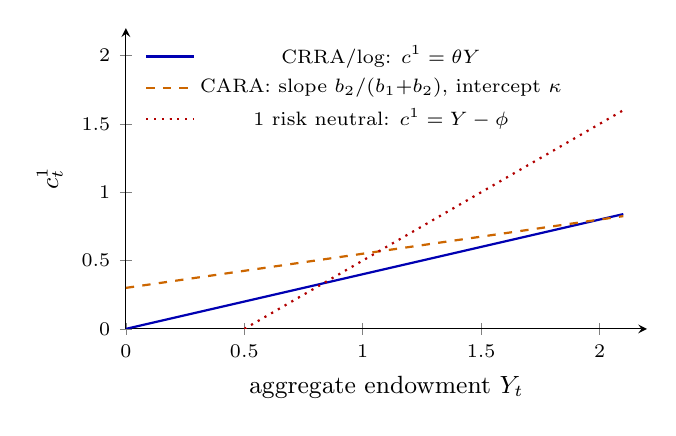
\begin{tikzpicture}
\begin{axis}[width=8.2cm,height=5.4cm,xmin=0,xmax=2.2,ymin=0,ymax=2.2,
  axis lines=left,xlabel={aggregate endowment $Y_t$},ylabel={$c^1_t$},
  xlabel style={font=\small},ylabel style={font=\small},tick label style={font=\scriptsize},
  legend style={font=\scriptsize,at={(0.02,0.98)},anchor=north west,draw=none,fill=none}]
  \addplot[blue!70!black,thick,domain=0:2.1]{0.4*x};
  \addlegendentry{CRRA/log: $c^1=\theta Y$}
  \addplot[orange!80!black,thick,dashed,domain=0:2.1]{0.25*x+0.3};
  \addlegendentry{CARA: slope $b_2/(b_1{+}b_2)$, intercept $\kappa$}
  \addplot[red!70!black,thick,dotted,domain=0.5:2.1]{x-0.5};
  \addlegendentry{1 risk neutral: $c^1=Y-\phi$}
\end{axis}
\end{tikzpicture}
\end{center}
\emph{How to read the figure.} The horizontal axis is aggregate endowment $Y_t$, the vertical axis is household 1's consumption. The slope of each line is the share of aggregate risk household 1 bears. With log/CRRA preferences it bears a constant proportion (ray through the origin); with CARA a constant slope plus a fixed transfer; if household 1 is risk neutral the slope is 1 and household 2's consumption $Y_t-c^1_t=\phi$ is flat.

\begin{tipbox}
CRRA (log) $\Rightarrow$ constant consumption \emph{shares}; CARA $\Rightarrow$ constant \emph{slopes} plus a transfer; a risk-neutral agent fully insures the risk-averse one. In every case only aggregate risk is shared --- idiosyncratic risk is fully diversified away under complete markets.
\end{tipbox}

%======================================================================
\subsection{Pricing redundant assets; the risk-neutral measure \pg{26}}

\paragraph{Setup.} Two dates as in the two-state example. States $s$ at date 1 occur with physical probabilities $\pi(s)$; AD prices $q(s)$ are known. A \emph{redundant asset} is any asset whose payoff $x(s)$ (in each state $s$) can be replicated by a portfolio of AD securities: hold $x(s)$ units of the AD security for state $s$.

\paragraph{No arbitrage.} Two portfolios with identical payoffs in every state must have the same price; otherwise one could buy the cheap one, sell the expensive one, and earn a riskless profit. Hence:
\begin{align*}
  P(x) &= \sum_s q(s)\,x(s) && \text{(cost of the replicating AD portfolio)}\\
  &= \sum_s \pi(s)\,\frac{q(s)}{\pi(s)}\,x(s) && \text{(multiply and divide by $\pi(s)$)}\\
  &= E\big[m\,x\big],\qquad m(s)\equiv\frac{q(s)}{\pi(s)}. && \text{(definition of expectation)}
\end{align*}
Using $q(s)=\beta\pi(s)u'(c(s))/u'(c_0)$ from the two-state example,
\[
  m(s)=\beta\,\frac{u'(c(s))}{u'(c_0)} = \text{IMRS (intertemporal marginal rate of substitution)}.
\]
$m$ is the stochastic discount factor: it measures how much the household values a payoff in each state. It is the static counterpart of $M_{t,t+1}$ in \eqref{eq:s4_sdf}.

\paragraph{Risk-free rate.} A risk-free bond pays $x(s)=1$ in every state. Its price is
\[
  \sum_sq(s)=\sum_s\pi(s)m(s)=E[m]\equiv\frac{1}{R_f}
  \quad\Longrightarrow\quad R_f=\frac{1}{E[m]} \quad\text{(HW3 Q2(c))}.
\]
The gross risk-free rate is the inverse of the expected IMRS.

\paragraph{Risk-neutral (equivalent martingale) measure.} Define
\[
  \pi^*(s)\equiv R_f\,q(s) = R_f\,\pi(s)\,m(s) = \frac{m(s)}{E[m]}\,\pi(s).
\]
Each $\pi^*(s)>0$ (since $q(s)>0$), and they sum to one:
$\sum_s\pi^*(s)=R_f\sum_sq(s)=R_f\cdot\frac{1}{R_f}=1$. So $\pi^*$ is a probability measure: the physical probabilities reweighted by $m(s)/E[m]$. Now rewrite the pricing formula:
\begin{align*}
  P(x) &= \sum_s q(s)\,x(s) = \sum_s \frac{\pi^*(s)}{R_f}\,x(s) && \text{(since $q(s)=\pi^*(s)/R_f$)}\\
       &= \frac{1}{R_f}\,E^*[x], && \text{($E^*$: expectation under $\pi^*$)}
\end{align*}
\begin{keybox}[title=Risk-neutral pricing]
\[
  P(x) = E[m\,x] = \frac{E^*[x]}{R_f},\qquad \pi^*(s)=\frac{m(s)}{E[m]}\,\pi(s).
\]
\begin{itemize}
  \item Risk-averse agents: $m(s)$ is high in bad states (low $c(s)$, high $u'$), so $\pi^*$ \emph{overweights bad states} and \emph{underweights good states}.
  \item Risk-neutral agents: $u'$ constant, so $m(s)=\beta$ for all $s$, $m(s)/E[m]=\beta/\beta=1$, and $\pi^*(s)=\pi(s)$. Prices are then simply discounted expected payoffs.
\end{itemize}
\end{keybox}
Interpretation: all risk adjustment can be put either into the discount factor ($E[mx]$ with physical probabilities) or into the probabilities ($E^*[x]/R_f$ with a risk-free discount rate). Both give the same price.

\paragraph{Numerical example.} Let $\pi(1)=\pi(2)=\tfrac12$, $\beta=0.95$, log utility, $c_0=1$, $c(1)=1.1$ (good state), $c(2)=0.9$ (bad state).
\begin{itemize}
  \item SDF: $m(1)=0.95/1.1\approx0.864$, \ $m(2)=0.95/0.9\approx1.056$; \ $E[m]\approx0.960$, so $R_f\approx1.042$.
  \item Risk-neutral probabilities: $\pi^*(s)=m(s)/(2E[m])$, giving $\pi^*(1)=\frac{1/1.1}{1/1.1+1/0.9}=0.45$ and $\pi^*(2)=0.55$. The bad state gets more weight than its physical probability $0.5$.
  \item Claim to consumption, $x(s)=c(s)$: $P=E[mx]=\tfrac12(0.95)+\tfrac12(0.95)=0.95$. Check: $E^*[x]/R_f=(0.45\cdot1.1+0.55\cdot0.9)/1.042=0.99/1.042\approx0.95$.
  \item Its expected return is $E[x]/P=1/0.95\approx1.053>R_f\approx1.042$: the asset pays off in good times, so it carries a risk premium.
\end{itemize}

\section{Heterogeneous Agents and Distributions}

This section studies economies in which households are hit by \emph{idiosyncratic} (individual-specific) income shocks that they cannot fully insure. Because different households experience different shock histories, they end up with different wealth levels, so the economy has a whole \emph{distribution} of agents rather than a single representative agent. We need two tools to describe it:
\begin{itemize}
  \item the \textbf{Hamilton--Jacobi--Bellman (HJB) equation}, which describes the optimal choices of one household, and
  \item the \textbf{Kolmogorov forward (KF) equation}, also called the Fokker--Planck equation, which describes how the cross-sectional distribution of households evolves given those choices.
\end{itemize}
Equilibrium then requires that the prices households take as given (the interest rate, the wage) clear markets once we aggregate over the distribution.

%--------------------------------------------------------------------
\subsection{Huggett model: motivation and setup \pg{39}}

\paragraph{Motivation.}
\begin{itemize}
  \item \textbf{Markets are incomplete.} In the data, only about one third of \emph{permanent} income shocks are insured through markets (or other arrangements); the rest passes through to consumption. A representative-agent model with complete markets cannot capture this.
  \item \textbf{Self-insurance.} In the Huggett model households cannot buy insurance against income shocks. Instead they \emph{self-insure}: they accumulate a \textbf{buffer stock of savings} in good times and run it down in bad times, which smooths consumption against idiosyncratic shocks.
  \item \textbf{Two sources of market incompleteness:}
    \begin{enumerate}
      \item the only asset available for saving or borrowing is a single \emph{risk-free bond} (no state-contingent claims, so no insurance contracts);
      \item there is a \emph{borrowing constraint}: households cannot borrow beyond a limit.
    \end{enumerate}
  \item \textbf{Two kinds of heterogeneity:}
    \begin{itemize}
      \item \emph{ex-ante}: agents differ in fixed characteristics from the start (e.g.\ different preferences or abilities);
      \item \emph{ex-post}: agents are identical ex-ante but become different because they receive different realisations of random shocks.
    \end{itemize}
    Huggett and Aiyagari models use \textbf{ex-post} heterogeneity: everybody faces the same income process, but luck differs.
\end{itemize}

\paragraph{Setup (continuous time).}
\begin{itemize}
  \item Time $t\ge0$ is continuous. There is a continuum of households of total mass $1$.
  \item $a_t$: a household's wealth (bond holdings) at time $t$. $a_t<0$ means the household is a borrower.
  \item $y_t$: the household's labour income (an endowment, no labour choice). It takes two values, $y_t\in\{y_1,y_2\}$ with $y_1<y_2$: $y_1$ is the ``bad'' state (e.g.\ unemployment) and $y_2$ the ``good'' state.
  \item Income follows a two-state \textbf{Poisson process}: a household in state $j$ jumps to the other state at rate $\lambda_j>0$, i.e.\ over a short interval of length $\Delta$ it switches with probability $\lambda_j\Delta$ and stays with probability $1-\lambda_j\Delta$ (up to terms of order $\Delta^2$). We write $-j$ for ``the other state'' (if $j=1$ then $-j=2$ and vice versa). Later the income process is generalised, e.g.\ to a diffusion.
  \item $c_t$: consumption, chosen by the household. $u(\cdot)$: instantaneous utility, strictly increasing and strictly concave ($u'>0$, $u''<0$). $\rho>0$: discount rate.
  \item $r$: the interest rate on the bond. The household takes $r$ as given; in equilibrium it is determined by market clearing.
  \item $\underline a$: the borrowing limit (exogenous).
\end{itemize}

The household solves
\begin{equation}\label{eq:hug-problem}
  \max_{\{c_t\}_{t\ge0}} \; E_0\!\int_0^\infty e^{-\rho t}u(c_t)\,dt
  \quad\text{s.t.}\quad
  \dot a_t = y_t + r a_t - c_t,\qquad a_t\ge \underline a ,
\end{equation}
where $\dot a_t\equiv da_t/dt$. The budget constraint says wealth grows by income plus interest minus consumption.

\paragraph{The borrowing limit and the natural borrowing limit.}
We require $\underline a\ge -y_1/r$ (for $r>0$). To see where $-y_1/r$ comes from, ask: what is the largest debt a household could \emph{surely} repay? In the worst case its income stays at $y_1$ forever. The present value of that income stream is
\begin{align*}
  \int_0^\infty e^{-rt}y_1\,dt
  &= y_1\Big[-\tfrac{1}{r}e^{-rt}\Big]_0^\infty &&\text{(integrate the exponential)}\\
  &= \frac{y_1}{r}. &&\text{(}e^{-rt}\to0\text{ as }t\to\infty\text{)}
\end{align*}
Even consuming (almost) nothing, the household can repay at most $y_1/r$, so lenders would never lend more: debt must satisfy $-a_t\le y_1/r$, i.e.\ $a_t\ge -y_1/r$. This is the \textbf{natural borrowing limit}. Any \emph{ad hoc} limit $\underline a$ must be at least as tight: $\underline a\ge -y_1/r$.
\begin{itemize}
  \item Special case $\underline a=0$: households can only save, never borrow.
\end{itemize}

\paragraph{Equilibrium concept.} In \textbf{general equilibrium}, bonds are in \textbf{zero net supply}: they are IOUs between households, so total borrowing must equal total lending, i.e.\ aggregate wealth is zero. The interest rate $r$ adjusts to make this hold.

%--------------------------------------------------------------------
\subsection{The HJB equation with Poisson income switching \pg{40}}

Let $v_j(a)$ be the value (maximised expected lifetime utility) of a household with wealth $a$ and current income $y_j$. Since the problem is stationary (nothing depends on calendar time given $r$), $v_j$ depends only on $(a,j)$.

\paragraph{Derivation (heuristic, via a short time step).}
Consider a short interval of length $\Delta$. The household consumes $c$, so wealth moves from $a$ to $a+\Delta(y_j+ra-c)$. With probability $1-\lambda_j\Delta$ income stays at $y_j$; with probability $\lambda_j\Delta$ it switches to $y_{-j}$. The discrete-time Bellman equation is
\begin{equation*}
  v_j(a)=\max_c\Big\{\Delta\,u(c) + e^{-\rho\Delta}\Big[(1-\lambda_j\Delta)\,v_j\big(a+\Delta s\big) + \lambda_j\Delta\, v_{-j}\big(a+\Delta s\big)\Big]\Big\},
  \qquad s\equiv y_j+ra-c.
\end{equation*}
Use the first-order approximations $e^{-\rho\Delta}\approx 1-\rho\Delta$ and $v_j(a+\Delta s)\approx v_j(a)+v_j'(a)\Delta s$ (Taylor expansion), and drop all terms of order $\Delta^2$:
\begin{align*}
  v_j(a) &= \max_c\Big\{\Delta u(c) + (1-\rho\Delta)\big[v_j(a)+v_j'(a)\Delta s - \lambda_j\Delta v_j(a) + \lambda_j\Delta v_{-j}(a)\big]\Big\}\\
  &= \max_c\Big\{\Delta u(c) + v_j(a) - \rho\Delta v_j(a) + v_j'(a)\Delta s + \lambda_j\Delta\big(v_{-j}(a)-v_j(a)\big)\Big\}.
\end{align*}
Subtract $v_j(a)$ from both sides, move $\rho\Delta v_j(a)$ to the left and divide by $\Delta$:
\begin{equation}\label{eq:hug-hjb}
  \rho v_j(a) = \max_c\Big\{u(c) + v_j'(a)\,(y_j+ra-c) + \lambda_j\big(v_{-j}(a)-v_j(a)\big)\Big\},\qquad j=1,2.
\end{equation}

\textbf{Reading the HJB.} The left side is the ``return'' on the value $v_j$ at rate $\rho$. The right side is the flow payoff: utility $u(c)$, plus the value of the change in wealth ($v_j'(a)\times\dot a$), plus the expected capital gain or loss from a switch in income: with intensity $\lambda_j$ the value jumps from $v_j(a)$ to $v_{-j}(a)$.

\paragraph{Optimal consumption.} Maximising the right side of \eqref{eq:hug-hjb} over $c$ gives the first-order condition
\begin{equation}\label{eq:hug-foc}
  u'\big(c_j(a)\big) = v_j'(a)\quad\Longrightarrow\quad c_j(a)=(u')^{-1}\big(v_j'(a)\big).
\end{equation}
The marginal utility of consuming one more unit equals the marginal value of keeping it as wealth. The implied \textbf{saving policy} in state $j$ is
\begin{equation}\label{eq:hug-saving}
  s_j(a)\equiv y_j + ra - c_j(a)\quad(=\dot a\text{ for a household in state }j\text{ with wealth }a).
\end{equation}

%--------------------------------------------------------------------
\subsection{Kolmogorov forward equation with Poisson shocks \pg{40}}

Given the policies $s_j(a)$, we now track how the population distributes itself over wealth and income.

\paragraph{Setup.}
\begin{itemize}
  \item $\tilde a_t,\tilde y_t$: wealth and income of a randomly drawn household at time $t$ (tildes denote random variables).
  \item Joint CDF in income state $j$:\quad $G_j(a,t)\equiv\Pr\big(\tilde a_t\le a,\ \tilde y_t=y_j\big)$.
  \item Density: $g_j(a,t)\equiv\partial_a G_j(a,t)$, so $g_j(a,t)\,da$ is the mass of households with income $y_j$ and wealth in $[a,a+da]$. Here $\partial_a$ and $\partial_t$ denote partial derivatives in the wealth and time dimensions.
  \item Note $G_1+G_2$ is the marginal CDF of wealth, and $\int (g_1+g_2)\,da=1$.
\end{itemize}

\paragraph{Step 1: the law of motion over a short interval.}
Over an interval of length $\Delta$, a household in state $j$ moves deterministically along its saving policy, $\tilde a_{t+\Delta}=\tilde a_t+\Delta\,s_j(\tilde a_t)$, and its income switches to $-j$ with probability $\lambda_j\Delta$.

Which households are in state $j$ with wealth $\le a$ at $t+\Delta$? Two groups:
\begin{itemize}
  \item households that were in $j$ and did \emph{not} switch (probability $1-\lambda_j\Delta$) and whose wealth satisfies $\tilde a_t+\Delta s_j(\tilde a_t)\le a$, i.e.\ (to first order) $\tilde a_t\le a-\Delta s_j(a)$;
  \item households that were in $-j$ and \emph{did} switch into $j$ (probability $\lambda_{-j}\Delta$), with $\tilde a_t\le a-\Delta s_{-j}(a)$.
\end{itemize}
Hence
\begin{equation}\label{eq:kf-discrete}
  G_j(a,t+\Delta) = (1-\lambda_j\Delta)\,G_j\big(a-\Delta s_j(a),t\big) + \lambda_{-j}\Delta\,G_{-j}\big(a-\Delta s_{-j}(a),t\big).
\end{equation}

\paragraph{Step 2: take the limit $\Delta\to0$.}
Taylor-expand in the wealth argument: $G_j(a-\Delta s_j(a),t)\approx G_j(a,t)-\Delta s_j(a)\,\partial_aG_j(a,t)$. Substitute into \eqref{eq:kf-discrete}:
\begin{align*}
  G_j(a,t+\Delta) &= (1-\lambda_j\Delta)\big[G_j(a,t)-\Delta s_j(a)\partial_aG_j(a,t)\big] + \lambda_{-j}\Delta\,G_{-j}(a,t) + O(\Delta^2)\\
  &= G_j(a,t) - \Delta s_j(a)\partial_aG_j(a,t) - \lambda_j\Delta G_j(a,t) + \lambda_{-j}\Delta G_{-j}(a,t) + O(\Delta^2).
\end{align*}
Subtract $G_j(a,t)$ from both sides and divide by $\Delta$:
\begin{equation*}
  \frac{G_j(a,t+\Delta)-G_j(a,t)}{\Delta} = - s_j(a)\partial_aG_j(a,t) - \lambda_j G_j(a,t) + \lambda_{-j} G_{-j}(a,t) + O(\Delta).
\end{equation*}
Let $\Delta\to0$; the left side becomes $\partial_tG_j(a,t)$:
\begin{equation}\label{eq:kf-cdf}
  \partial_t G_j(a,t) = -s_j(a)\,\partial_a G_j(a,t) - \lambda_j G_j(a,t) + \lambda_{-j}G_{-j}(a,t).
\end{equation}

\paragraph{Step 3: from the CDF to the density.}
Differentiate \eqref{eq:kf-cdf} with respect to $a$. On the left, $\partial_a\partial_tG_j=\partial_t\partial_aG_j=\partial_t g_j$. On the right, $\partial_a\big[s_j(a)\partial_aG_j\big]=\partial_a\big[s_j(a)g_j\big]$ and $\partial_aG_{\pm j}=g_{\pm j}$. Therefore
\begin{keybox}[title=Kolmogorov forward equation (two-state Poisson income)]
\begin{equation}\label{eq:kf-density}
  \partial_t g_j(a,t) = -\partial_a\big[s_j(a)\,g_j(a,t)\big] \;-\; \underbrace{\lambda_j g_j(a,t)}_{\text{outflow from }j} \;+\; \underbrace{\lambda_{-j}g_{-j}(a,t)}_{\text{inflow from }-j},\qquad j=1,2.
\end{equation}
\end{keybox}
\textbf{Interpretation.} The density at $(a,j)$ changes for two reasons. (i) \emph{Drift in the wealth dimension}: $-\partial_a[s_jg_j]$ is minus the derivative of the flow of households moving through wealth level $a$ (the ``flux'' $s_jg_j$); if more households flow out of a small wealth interval than flow in, the density there falls. (ii) \emph{Jumps in the income dimension}: households in $j$ leave at rate $\lambda_j$, and households in $-j$ arrive at rate $\lambda_{-j}$.

\paragraph{Implied stationary income distribution.}
Let $\pi_j(t)\equiv\int g_j(a,t)\,da$ be the share of households in income state $j$. Integrate \eqref{eq:kf-density} over all $a$. The drift term integrates to the net flux through the boundaries of the wealth space, $-[s_jg_j]_{\underline a}^{\infty}$, which is zero because no household leaves the state space (at $\underline a$ wealth cannot fall, and $g_j\to0$ as $a\to\infty$). So
\begin{equation*}
  \dot\pi_j(t) = -\lambda_j\pi_j(t)+\lambda_{-j}\pi_{-j}(t).
\end{equation*}
In a stationary state $\dot\pi_j=0$, so $\lambda_1\pi_1=\lambda_2\pi_2$; with $\pi_1+\pi_2=1$ this gives
\begin{equation}\label{eq:pi-stat}
  \pi_1=\frac{\lambda_2}{\lambda_1+\lambda_2},\qquad \pi_2=\frac{\lambda_1}{\lambda_1+\lambda_2}.
\end{equation}
The flow out of the bad state equals the flow into it; the bad state is more common when it is hard to leave ($\lambda_1$ small) and easy to enter ($\lambda_2$ large).

%--------------------------------------------------------------------
\subsection{Huggett stationary equilibrium \pg{40}}

A \textbf{stationary} equilibrium is one in which the distribution no longer changes over time: $\partial_t g_j(a,t)=0$. We then drop the $t$ argument and write $g_j(a)$. Setting the left side of \eqref{eq:kf-density} to zero removes the time dimension, and the partial derivative in $a$ becomes an ordinary derivative.

\begin{keybox}[title=Huggett stationary equilibrium]
An interest rate $r$, value functions $v_j$, policies $c_j,s_j$ and densities $g_j$ ($j=1,2$) such that:
\begin{align}
  \text{(HJB)}\quad & \rho v_j(a) = \max_c\Big\{u(c) + v_j'(a)\,(y_j+ra-c) + \lambda_j\big(v_{-j}(a)-v_j(a)\big)\Big\},\label{eq:hug-eq-hjb}\\
  \text{(KF)}\quad & 0 = -\frac{d}{da}\big[s_j(a)\,g_j(a)\big] - \lambda_j g_j(a) + \lambda_{-j}g_{-j}(a),\label{eq:hug-eq-kf}\\
  \text{(density)}\quad & \int_{\underline a}^\infty \big(g_1(a)+g_2(a)\big)\,da = 1,\qquad g_1,g_2\ge 0,\label{eq:hug-eq-dens}\\
  \text{(bond market)}\quad & S(r) \equiv \int_{\underline a}^\infty a\,g_1(a)\,da + \int_{\underline a}^\infty a\,g_2(a)\,da = 0,\label{eq:hug-eq-mkt}
\end{align}
with $s_j(a)=y_j+ra-c_j(a)$ and $u'(c_j(a))=v_j'(a)$ from \eqref{eq:hug-foc}.
\end{keybox}
\begin{itemize}
  \item The HJB gives individual behaviour for a given $r$; the KF equation aggregates that behaviour into a distribution; the density condition normalises total mass to one.
  \item $S(r)$ is aggregate wealth (aggregate saving) at interest rate $r$. Because bonds are in zero net supply, $S(r)=0$: total lending (positive $a$) equals total borrowing (negative $a$).
  \item The system is recursive in $r$: given $r$ we can solve \eqref{eq:hug-eq-hjb}, then \eqref{eq:hug-eq-kf}--\eqref{eq:hug-eq-dens}, then evaluate $S(r)$. Equilibrium is the $r$ that sets $S(r)=0$.
\end{itemize}

%--------------------------------------------------------------------
\subsection{The borrowing constraint as a boundary condition \pg{40--41}}

The constraint $a\ge\underline a$ is imposed at the \textbf{lower boundary} of the wealth space, as a condition on the value function at $a=\underline a$. This is how it enters the numerical (finite-difference) code.

\paragraph{Step 1: saving at the constraint cannot be negative.}
A household sitting exactly at $a=\underline a$ cannot let its wealth fall further. So its saving there must be non-negative:
\begin{equation}\label{eq:bc-saving}
  s_j(\underline a) = y_j + r\underline a - c_j(\underline a) \;\ge\; 0 .
\end{equation}
If instead $s_j(\underline a)<0$, wealth would fall below $\underline a$ an instant later, which is impossible in the model.

\paragraph{Step 2: translate into a condition on $v_j'(\underline a)$.}
Rearranging \eqref{eq:bc-saving}: $c_j(\underline a)\le y_j+r\underline a$. Since $u$ is concave, $u'$ is decreasing, so a smaller argument gives a larger marginal utility:
\begin{align*}
  c_j(\underline a)\le y_j+r\underline a
  &\;\Longrightarrow\; u'\big(c_j(\underline a)\big)\ \ge\ u'\big(y_j+r\underline a\big) &&\text{(}u'\text{ decreasing)}\\
  &\;\Longrightarrow\; v_j'(\underline a)\ \ge\ u'\big(y_j+r\underline a\big). &&\text{(FOC \eqref{eq:hug-foc} at }a=\underline a\text{)}
\end{align*}
\begin{keybox}[title=State-constraint boundary condition]
\begin{equation}\label{eq:state-constraint}
  v_j'(\underline a)\;\ge\;u'\big(y_j+r\underline a\big),\qquad j=1,2.
\end{equation}
\end{keybox}
\textbf{Interpretation.} At the borrowing limit the marginal value of wealth is at least the marginal utility of consuming all current income. In practice, in the finite-difference scheme the derivative at the boundary is set to $v_j'(\underline a)=u'(y_j+r\underline a)$ whenever the unconstrained choice would imply dissaving, which forces $c_j(\underline a)= y_j+r\underline a$ and $s_j(\underline a)=0$. Typically the constraint binds for low-income households: they would like to borrow more but cannot, and a mass of them sits at $\underline a$.

%--------------------------------------------------------------------
\subsection{Variations: Huggett, Bewley and Aiyagari \pg{41--42}}

All three models share the same household block (HJB + KF); they differ in \emph{what the asset is} and therefore in the market-clearing condition. Write $A(r)$ for aggregate household asset demand at interest rate $r$ (in Huggett, $A(r)=S(r)$ from \eqref{eq:hug-eq-mkt}).

\subsubsection*{(a) Huggett: assets in zero net supply}
Equilibrium condition: $A(r)=0$. \textbf{Computation} by iterating on the interest rate:
\begin{enumerate}
  \item Guess $r$.
  \item Solve the HJB \eqref{eq:hug-eq-hjb} for $v_j$, hence $c_j(a)$ and $s_j(a)$.
  \item Solve the KF equation \eqref{eq:hug-eq-kf} with \eqref{eq:hug-eq-dens} for $g_j$.
  \item Compute $S(r)$ from \eqref{eq:hug-eq-mkt}.
  \item If $S(r)>0$ (excess saving), lower $r$; if $S(r)<0$ (excess borrowing), raise $r$. Return to step 2 until $S(r)\approx0$ (e.g.\ by bisection).
\end{enumerate}
This works because $S(r)$ is increasing in $r$: a higher return makes households save more and borrow less.

\begin{center}
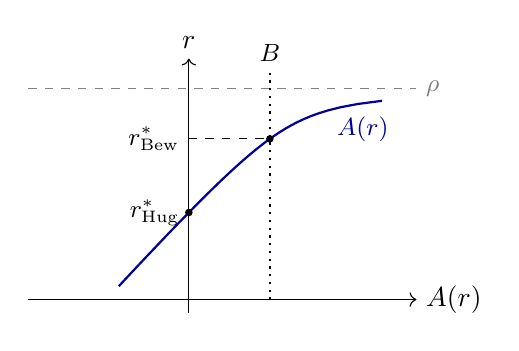
\begin{tikzpicture}[scale=0.85]
  \draw[->] (-2.4,0)--(3.4,0) node[right]{$A(r)$};
  \draw[->] (0,-0.2)--(0,3.6) node[above]{$r$};
  \draw[dashed,gray] (-2.4,3.15)--(3.4,3.15) node[right]{\small $\rho$};
  \draw[thick,blue!60!black,domain=0.2:2.97,samples=60,variable=\t]
     plot ({0.15*(\t-1.3)/(3.15-\t)+0.9*(\t-1.3)},{\t});
  \node[blue!60!black] at (2.6,2.55) {\small $A(r)$};
  \fill (0,1.3) circle (1.6pt) node[left]{\small $r^*_{\text{Hug}}$};
  \draw[dotted,thick] (1.21,0)--(1.21,3.4) node[above]{\small $B$};
  \fill (1.21,2.4) circle (1.6pt);
  \draw[dashed] (0,2.4)--(1.21,2.4);
  \node[left] at (0,2.4) {\small $r^*_{\text{Bew}}$};
\end{tikzpicture}
\end{center}
\textbf{How to read the figure.} The horizontal axis is aggregate asset demand, the vertical axis the interest rate. The curve $A(r)$ slopes up because a higher $r$ raises saving; it diverges to $+\infty$ as $r\uparrow\rho$ because when the return on saving approaches the rate of time preference, households keep accumulating buffer-stock wealth without bound. Huggett's equilibrium is where $A(r)$ crosses the vertical axis ($A=0$); with positive bond supply $B$ (Bewley, below) the equilibrium is where $A(r)$ meets the vertical line at $B$, so $r^*_{\text{Bew}}>r^*_{\text{Hug}}$.

\subsubsection*{(b) Bewley: assets in positive supply}
\textbf{Setup.}
\begin{itemize}
  \item The government issues an exogenous amount $B>0$ of bonds, which households hold. A larger $B$ affects the equilibrium $r$ (see figure).
  \item It finances interest payments $rB$ and government spending $G$ by collecting taxes according to a tax function $\tau(a,y)$ (tax paid by a household with wealth $a$ and income $y$).
  \item $g(a,y_j;r)$: stationary density over $(a,y_j)$ when the interest rate is $r$ (same as $g_j(a)$ above, with the dependence on $r$ made explicit).
\end{itemize}
\textbf{Conditions.}
\begin{align*}
  \text{Total tax revenue:}\quad & T(r)=\sum_j\int_a \tau(a,y_j)\,g(a,y_j;r)\,da,\\
  \text{Government budget constraint:}\quad & G(r)+rB=T(r),\\
  \text{Asset market clearing:}\quad & A(r)=B.
\end{align*}
Given $B$ and the tax function, spending $G(r)$ is whatever the budget constraint allows. Households must now be willing to hold the positive stock $B$, which requires a higher interest rate than in Huggett.

\subsubsection*{(c) Aiyagari: adding production}
\textbf{Setup.}
\begin{itemize}
  \item A representative firm with constant-returns-to-scale (CRS) technology, and no aggregate shocks:
  $Y=K^\alpha L^{1-\alpha}$, $0<\alpha<1$; $K$: capital, $L$: effective labour.
  \item Capital depreciates at rate $\delta$. The firm rents capital at rental rate $r+\delta$ (households earn $r$ net of depreciation) and hires labour at wage $w$. Markets are competitive.
  \item Households own the capital: their wealth $a$ is now claims on $K$, so the asset is in \emph{positive} supply determined by the firm's demand for capital.
\end{itemize}

\paragraph{Firm optimisation.} The firm solves $\max_{K,L}\ K^\alpha L^{1-\alpha}-(r+\delta)K-wL$. The first-order conditions set factor prices equal to marginal products:
\begin{align}
  \partial_K:\quad & r+\delta=\alpha K^{\alpha-1}L^{1-\alpha}=\alpha\Big(\frac{K}{L}\Big)^{\alpha-1},\label{eq:aiy-r}\\
  \partial_L:\quad & w=(1-\alpha)K^{\alpha}L^{-\alpha}=(1-\alpha)\Big(\frac{K}{L}\Big)^{\alpha}.\label{eq:aiy-w}
\end{align}
Solve \eqref{eq:aiy-r} for the capital--labour ratio:
\begin{align*}
  \Big(\frac{K}{L}\Big)^{\alpha-1}&=\frac{r+\delta}{\alpha}
  &&\text{(divide by }\alpha\text{)}\\
  \frac{K}{L}&=\Big(\frac{r+\delta}{\alpha}\Big)^{\frac{1}{\alpha-1}}=\Big(\frac{\alpha}{r+\delta}\Big)^{\frac{1}{1-\alpha}}.
  &&\text{(raise to the power }1/(\alpha-1)\text{)}
\end{align*}
Substitute into \eqref{eq:aiy-w}:
\begin{equation}\label{eq:aiy-wr}
  w(r)=(1-\alpha)\Big(\frac{\alpha}{r+\delta}\Big)^{\frac{\alpha}{1-\alpha}}.
\end{equation}
So the wage is pinned down by $r$ alone (CRS means only the ratio $K/L$ matters), and $w'(r)<0$: a higher cost of capital means less capital per worker and a lower wage. Hence the whole model can again be solved by iterating on a single price $r$.

\paragraph{Household problem (discrete-time version).} With labour productivity $y_j$ (the household supplies $y_j$ efficiency units of labour inelastically), the budget constraint is
\begin{equation*}
  c+a'=w\,y_j+(1+r)a,\qquad a'\ge\underline a,
\end{equation*}
where $a'$ is next period's wealth. The household problem is exactly Huggett's, with income $w y_j$ instead of $y_j$.

\paragraph{Two market-clearing conditions.}
\begin{itemize}
  \item \textbf{Labour market} (labour supply is exogenous):
  \begin{equation}\label{eq:aiy-L}
    L=\sum_j\int_a y_j\,g(a,y_j;r)\,da=\sum_j y_j\int_a g(a,y_j;r)\,da=\sum_j y_j\pi_j,
  \end{equation}
  where $\pi_j\equiv\int_a g(a,y_j;r)\,da$ is the stationary share of households with productivity $y_j$ (for the two-state Poisson process, \eqref{eq:pi-stat}). Since $\pi_j$ depends only on the exogenous income process, $L$ does not depend on $r$.
  \item \textbf{Capital market}: household asset supply equals firm capital demand. Multiplying the capital--labour ratio by $L$,
  \begin{equation}\label{eq:aiy-K}
    A(r)=K(r)\equiv L\Big(\frac{\alpha}{r+\delta}\Big)^{\frac{1}{1-\alpha}}.
  \end{equation}
\end{itemize}

\begin{center}
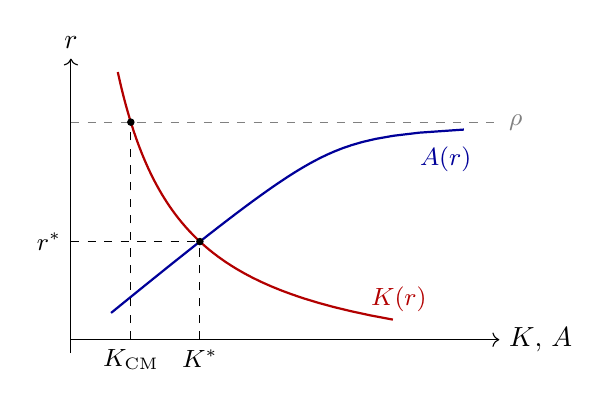
\begin{tikzpicture}[scale=0.85]
  \draw[->] (0,0)--(6.4,0) node[right]{$K$, $A$};
  \draw[->] (0,-0.2)--(0,4.2) node[above]{$r$};
  \draw[dashed,gray] (0,3.25)--(6.4,3.25) node[right]{\small $\rho$};
  \draw[thick,blue!60!black,domain=0.4:3.14,samples=60,variable=\t]
     plot ({0.6+1.2*(\t-0.4)+0.08*(\t-0.4)/(3.25-\t)},{\t});
  \node[blue!60!black] at (5.6,2.7) {\small $A(r)$};
  \draw[thick,red!70!black,domain=0.3:4.0,samples=60,variable=\t]
     plot ({4.6/(\t+0.6)-0.3},{\t});
  \node[red!70!black] at (4.9,0.6) {\small $K(r)$};
  \fill (1.927,1.466) circle (1.6pt);
  \draw[dashed] (0,1.466)--(1.927,1.466); \node[left] at (0,1.466) {\small $r^*$};
  \draw[dashed] (1.927,0)--(1.927,1.466); \node[below] at (1.927,0) {\small $K^*$};
  \fill (0.895,3.25) circle (1.6pt);
  \draw[dashed] (0.895,0)--(0.895,3.25); \node[below] at (0.895,0) {\small $K_{\text{CM}}$};
\end{tikzpicture}
\end{center}
\textbf{How to read the figure.} The red curve $K(r)$ is firms' capital demand from \eqref{eq:aiy-K}; it slopes down because a higher rental cost lowers the desired capital stock. The blue curve $A(r)$ is households' aggregate asset supply from the HJB+KF block; it slopes up and explodes as $r\uparrow\rho$. Their intersection gives $(r^*,K^*)$. Under complete markets (representative agent) the steady-state interest rate would be $r=\rho$, giving the smaller capital stock $K_{\text{CM}}$ where $K(r)$ reaches $\rho$; precautionary saving pushes $r^*<\rho$ and $K^*>K_{\text{CM}}$.

\paragraph{Continuous-time Aiyagari with diffusion income.}
\textbf{Setup.} Replace the two-state income process by a continuous productivity $z\in[z_{\min},z_{\max}]$ following a diffusion
\begin{equation*}
  dz_t=\mu(z_t)\,dt+\sigma(z_t)\,dW_t,
\end{equation*}
where $\mu(z)$ is the drift, $\sigma(z)$ the volatility, and $W_t$ a standard Brownian motion. Labour income is $wz$, so wealth evolves as $\dot a=wz+ra-c$, and the saving policy is $s(a,z)=wz+ra-c(a,z)$. The value function is $V(a,z)$ and the stationary density $g(a,z)$.

\emph{Ito's lemma} (used for the HJB): if $dz=\mu\,dt+\sigma\,dW$ and $a$ moves deterministically, then $E[dV]=\big(\partial_aV\,\dot a+\mu\,\partial_zV+\tfrac12\sigma^2\partial_{zz}V\big)dt$. Replacing the Poisson jump term in \eqref{eq:hug-hjb} by this expected drift of $V$ gives the HJB below. The KF equation is the ``adjoint'' of the HJB operator: each derivative acting on $V$ becomes a derivative of (coefficient $\times\, g$) with the sign flipped for first derivatives.

\begin{keybox}[title={Aiyagari stationary system (continuous time, diffusion income)}]
\begin{align}
  \text{(HJB)}\quad & \rho V(a,z) = \max_c\Big\{u(c) + \partial_aV(a,z)\,(wz+ra-c) + \mu(z)\,\partial_zV(a,z) \notag\\
  &\hspace{8.5em} + \tfrac12\sigma^2(z)\,\partial_{zz}V(a,z)\Big\},\label{eq:aiy-hjb}\\
  \text{(KF)}\quad & 0 = -\partial_a\big[s(a,z)g(a,z)\big] - \partial_z\big[\mu(z)g(a,z)\big] + \tfrac12\partial_{zz}\big[\sigma^2(z)g(a,z)\big],\label{eq:aiy-kf}\\
  \text{(density)}\quad & 1 = \int_{z_{\min}}^{z_{\max}}\!\!\int_{\underline a}^\infty g(a,z)\,da\,dz,\label{eq:aiy-dens}\\
  \text{(capital supply)}\quad & K = \int_{z_{\min}}^{z_{\max}}\!\!\int_{\underline a}^\infty a\,g(a,z)\,da\,dz,\label{eq:aiy-Ksupply}\\
  \text{(market clearing)}\quad & K = L\Big(\frac{\alpha}{r+\delta}\Big)^{\frac{1}{1-\alpha}},\qquad L=\int_{z_{\min}}^{z_{\max}}\!\!\int_{\underline a}^\infty z\,g(a,z)\,da\,dz,\label{eq:aiy-clear}
\end{align}
with $w=w(r)$ from \eqref{eq:aiy-wr}, the FOC $u'(c(a,z))=\partial_aV(a,z)$, and the state-constraint condition $\partial_aV(\underline a,z)\ge u'(wz+r\underline a)$.
\end{keybox}
\textbf{Interpretation.} \eqref{eq:aiy-kf} is \eqref{eq:kf-density} with the Poisson jump terms replaced by drift and diffusion in $z$, and $\partial_t g=0$ imposed. The first integral normalises the distribution; the second aggregates household wealth into the capital stock; the last line requires that this capital equals what firms demand at $r$.

\begin{tipbox}
The algorithm is always the same: guess the price $r$ (and hence $w(r)$) $\to$ solve the HJB $\to$ solve the KF equation $\to$ aggregate $\to$ check market clearing ($A=0$, $A=B$ or $A=K(r)$) $\to$ update $r$. Precautionary saving pushes $r$ below $\rho$: at $r=\rho$ households facing uninsurable risk and a borrowing limit would accumulate wealth without bound, so asset supply can equal any finite demand only at some $r<\rho$. In Aiyagari this means $K$ exceeds its complete-markets level.
\end{tipbox}

%--------------------------------------------------------------------
\subsection{Power laws, Pareto distribution and Zipf's law \pg{96}}

Many economic size variables (wealth, firm size, city size) have very fat right tails. Power laws are the standard way to describe them.

\paragraph{Setup.}
\begin{itemize}
  \item $S$: a positive random variable (``size''), with realisations $s$.
  \item $s_m>0$: the minimum possible value of $s$ (the scale parameter).
  \item $\alpha>0$: the shape (tail) parameter.
  \item $N$: number of observations (e.g.\ number of cities).
\end{itemize}

\paragraph{Pareto distribution.} The density is
\begin{equation}\label{eq:pareto-pdf}
  f(s)=\frac{\alpha s_m^\alpha}{s^{\alpha+1}}=\alpha s_m^\alpha s^{-\alpha-1},\qquad s\ge s_m.
\end{equation}
\emph{CDF.} Integrate the density from the minimum:
\begin{align*}
  F(s)&=\int_{s_m}^{s}\alpha s_m^\alpha x^{-\alpha-1}\,dx\\
  &=\alpha s_m^\alpha\Big[\frac{x^{-\alpha}}{-\alpha}\Big]_{s_m}^{s} &&\text{(antiderivative of }x^{-\alpha-1}\text{)}\\
  &=s_m^\alpha\big(s_m^{-\alpha}-s^{-\alpha}\big)\\
  &=1-\Big(\frac{s_m}{s}\Big)^\alpha.
\end{align*}
\emph{Survival function} (probability of exceeding $s$):
\begin{equation}\label{eq:pareto-surv}
  \bar S(s)\equiv\Pr(S>s)=1-F(s)=\Big(\frac{s_m}{s}\Big)^\alpha .
\end{equation}
Taking logs,
\begin{equation}\label{eq:pareto-logsurv}
  \log\bar S(s)=\alpha\log\Big(\frac{s_m}{s}\Big)=\alpha\log s_m-\alpha\log s .
\end{equation}
\begin{itemize}
  \item The Pareto is a \textbf{long-tailed} distribution: $\bar S(s)$ decays only like a power of $s$, not exponentially.
  \item $\alpha\uparrow\Rightarrow$ the survival function falls faster $\Rightarrow$ thinner tail $\Rightarrow$ lower probability of extreme values. (The mean is finite only if $\alpha>1$, the variance only if $\alpha>2$.)
\end{itemize}

\paragraph{Rank--size relation.}
With $N$ observations, the \textbf{rank} $R(s)$ of an observation of size $s$ is the number of observations larger than $s$ (the largest has rank $\approx1$). For large $N$ this is $N$ times the probability of exceeding $s$:
\begin{equation}\label{eq:rank}
  R(s)=N\,\bar S(s)=N\Big(\frac{s_m}{s}\Big)^\alpha .
\end{equation}
Take logs of \eqref{eq:rank} and use \eqref{eq:pareto-logsurv}:
\begin{align*}
  \log R(s)&=\log N+\log\bar S(s)\\
  &=\underbrace{\log N+\alpha\log s_m}_{\text{constant}}-\alpha\log s .
\end{align*}
\begin{keybox}[title=Log rank vs.\ log size]
Under a Pareto distribution, a plot of $\log(\text{rank})$ against $\log(\text{size})$ is a \textbf{straight line with slope $-\alpha$}. This is how the tail exponent is estimated in practice.
\end{keybox}

\paragraph{Power law (PL).} A more general way to state the same idea: $S$ follows a power law if there exist constants $k,\zeta>0$ such that
\begin{equation}\label{eq:pl}
  \Pr(S>x)=k\,x^{-\zeta}\qquad\text{for all } x\ge x_m,
\end{equation}
where $x_m\equiv k^{1/\zeta}$. The restriction $x\ge x_m$ is needed: a probability cannot exceed one, and $kx^{-\zeta}\le1\iff x\ge k^{1/\zeta}$. In empirical work ``power law'' usually means \eqref{eq:pl} holds in the upper tail (for large $x$).
\begin{itemize}
  \item $\zeta$ smaller $\Rightarrow$ $\Pr(S>x)$ decays more slowly $\Rightarrow$ fatter tail $\Rightarrow$ more inequality (more mass in very large values).
  \item \textbf{Relation to Pareto.} Comparing \eqref{eq:pl} with \eqref{eq:pareto-surv}, $(x_m/x)^\alpha=x_m^\alpha x^{-\alpha}$, so the Pareto distribution is the power law with $\zeta=\alpha$ and $k=x_m^{\zeta}$. Conversely an exact power law on $[x_m,\infty)$ is a Pareto distribution; a variable that only satisfies \eqref{eq:pl} in its tail is ``Pareto in the tail''.
\end{itemize}

\paragraph{Zipf's law.} Zipf's law is the special case $\zeta=1$:
\begin{equation*}
  \Pr(S>x)=\frac{k}{x}\;\propto\;\frac1x :
\end{equation*}
the probability that the variable exceeds a threshold $x$ is inversely proportional to $x$.

\emph{Equivalent rank form.} Let $S_{(r)}$ denote the size of the element with rank $r$ ($r$-th largest). By \eqref{eq:rank}, $r=N\Pr(S>S_{(r)})=N k\,S_{(r)}^{-\zeta}$. Solve for $S_{(r)}$:
\begin{align*}
  S_{(r)}^{\zeta}&=\frac{Nk}{r} &&\text{(multiply by }S_{(r)}^{\zeta}/r\text{)}\\
  S_{(r)}&=\Big(\frac{Nk}{r}\Big)^{1/\zeta}\;\propto\;r^{-1/\zeta}. &&\text{(raise to the power }1/\zeta\text{)}
\end{align*}
Under Zipf ($\zeta=1$) this becomes $S_{(r)}\propto 1/r$: the size (or frequency) of an element is \textbf{inversely proportional to its rank}. The 2nd largest is half the size of the largest, the 3rd largest a third, and so on.

\paragraph{The city size ``puzzle''.} City sizes follow a power law with exponent $\zeta\approx1$, i.e.\ Zipf's law.
\begin{center}
\begin{tikzpicture}[scale=0.8]
  \draw[->] (0,0)--(5,0) node[right]{\small $\ln$ population};
  \draw[->] (0,0)--(0,3.6) node[above]{\small $\ln$ rank};
  \foreach \x/\y in {0.7/2.95,1.1/2.62,1.5/2.40,1.9/2.08,2.3/1.85,2.7/1.52,3.1/1.30,3.5/0.98,3.9/0.72,4.2/0.55}
    \fill[gray] (\x,\y) circle (1.3pt);
  \draw[thick,blue!60!black] (0.5,3.1)--(4.4,0.4) node[right]{\small slope $\approx-1$};
\end{tikzpicture}
\end{center}
\textbf{How to read the figure.} Each dot is a city: horizontal position is log population, vertical position is log rank (the largest city has rank 1, so $\ln\text{rank}=0$ at the far right). By the keybox above, under a power law the dots lie on a straight line whose slope is $-\zeta$. For US cities (Gabaix 1999) the fitted line is
\begin{equation*}
  \ln\text{rank}=10.53-1.005\,\ln\text{size},
\end{equation*}
so $\zeta\approx1$: Zipf's law holds almost exactly.
\begin{tipbox}
The puzzle is \emph{why} the exponent is so close to exactly 1. Standard explanation (Gabaix): Gibrat's law, i.e.\ cities grow at random rates whose distribution is independent of their size, plus a lower reflecting barrier, generates a Pareto steady-state distribution with $\zeta\to1$.
\end{tipbox}

\section{Business Cycles: Detrending and the RBC Model}

This section has two parts. First, we explain how economists separate a macroeconomic time series into a slow-moving \emph{trend} and a \emph{cyclical} component (linear detrending and the Hodrick--Prescott filter). Second, we build and solve the basic \emph{Real Business Cycle} (RBC) model, whose job is to explain the cyclical component.

%=====================================================================
\subsection{Business cycles and linear detrending \pg{43}}

\paragraph{Setup.}
\begin{itemize}
  \item Time is discrete, $t=1,2,\dots,T$ (e.g.\ quarters or years).
  \item $x_t>0$: an observed macro series in levels (e.g.\ real GDP).
  \item \textbf{Business cycle} = the deviation of a series from its trend. Because real GDP grows over time, we must first remove the trend component; what remains is the cycle that business-cycle models try to explain.
\end{itemize}

\paragraph{Method 1: linear (log-linear) detrending.}
Assume the series is the \emph{product} of a deterministic exponential trend and a cyclical factor:
\begin{equation}\label{eq:s6_lintrend}
x_t=\underbrace{x_0e^{\gamma t}}_{\text{trend}}\cdot\underbrace{\bar x_t}_{\text{cycle}} ,
\end{equation}
where
\begin{itemize}
  \item $x_0>0$ is the trend level at $t=0$;
  \item $\gamma$ is the constant trend growth rate (since $\frac{d}{dt}\ln(x_0e^{\gamma t})=\gamma$);
  \item $\bar x_t>0$ is the cyclical factor: $\bar x_t>1$ means the series is above trend (expansion), $\bar x_t<1$ below trend (contraction), $\bar x_t=1$ exactly on trend.
\end{itemize}
Take natural logs of \eqref{eq:s6_lintrend}, using $\ln(ab)=\ln a+\ln b$ and $\ln e^{\gamma t}=\gamma t$:
\begin{align}
\ln x_t&=\ln x_0+\ln e^{\gamma t}+\ln\bar x_t \notag\\
&=\underbrace{\ln x_0}_{a}+\underbrace{\gamma}_{b}\,t+\underbrace{\ln\bar x_t}_{e_t}. \label{eq:s6_linreg}
\end{align}
This is a linear regression of $\ln x_t$ on a constant and a time trend, $\ln x_t=a+bt+e_t$.
\begin{itemize}
  \item Estimate $a$ and $b$ by OLS: $\hat b=\dfrac{\sum_t(t-\bar t)(\ln x_t-\overline{\ln x})}{\sum_t(t-\bar t)^2}$, $\hat a=\overline{\ln x}-\hat b\,\bar t$ (bars denote sample means).
  \item The cyclical component is the OLS residual: the fitted trend is \emph{subtracted from} the series,
  \[
  \ln\bar x_t=\ln x_t-\hat a-\hat b\,t .
  \]
  Since $\ln\bar x_t\approx\bar x_t-1$ for $\bar x_t$ near 1, the residual is approximately the percentage deviation from trend.
  \item \textbf{Problem:} real series contain a \emph{stochastic} trend (permanent shocks shift the level of GDP for good). A straight line cannot follow such shifts, so part of the permanent component stays in the residual. The resulting ``cycle'' is too persistent: measured cycles last too long.
\end{itemize}

%=====================================================================
\subsection{The Hodrick--Prescott (HP) filter \pg{43--44}}

\paragraph{Setup.}
\begin{itemize}
  \item $y_t$: the \emph{log} of the observed series at date $t$, for $t=1,\dots,T$ (data, taken as given).
  \item $y_t^g$: the trend (``growth'') component at $t$. The whole path $\{y_t^g\}_{t=1}^T$ is the choice variable.
  \item $y_t^c\equiv y_t-y_t^g$: the cyclical component (the part of the data the trend does not explain).
  \item $\mu\ge0$: a bound on how much the trend's growth rate may change; $\lambda\ge0$: the associated Lagrange multiplier, called the \emph{smoothing parameter}.
\end{itemize}
The HP trend is \emph{not} linear: it is allowed to bend slowly, so it also absorbs a slowly moving stochastic growth component that linear detrending misses.

\paragraph{The problem.} Choose the trend path to stay close to the data, subject to the trend being smooth:
\begin{equation}\label{eq:s6_hp}
\min_{\{y_t^g\}_{t=1}^T}\ \sum_{t=1}^T\left(y_t-y_t^g\right)^2
\quad\text{s.t.}\quad
\sum_{t=2}^{T-1}\Big[(y_{t+1}^g-y_t^g)-(y_t^g-y_{t-1}^g)\Big]^2\le\mu .
\end{equation}
\begin{itemize}
  \item $y_{t+1}^g-y_t^g$ is the trend growth rate between $t$ and $t+1$ (a log difference).
  \item $(y_{t+1}^g-y_t^g)-(y_t^g-y_{t-1}^g)=y_{t+1}^g-2y_t^g+y_{t-1}^g$ is the \emph{second difference}: the change in the trend growth rate. A straight line has all second differences equal to zero.
  \item In words: minimize the sum of squared deviations of the trend from the data, subject to the sum of squared second differences (how much trend growth changes) not being too large.
\end{itemize}

\paragraph{Lagrangian.}
\begin{equation}\label{eq:s6_hpL}
\mathcal L=\underbrace{\sum_{t=1}^{T}(y_t-y_t^g)^2}_{\text{(i) fit}}
+\underbrace{\lambda\Big[\sum_{t=2}^{T-1}\big(y_{t+1}^g-2y_t^g+y_{t-1}^g\big)^2-\mu\Big]}_{\text{(ii) smoothness}} .
\end{equation}
\begin{itemize}
  \item Think of $\mathcal L$ as a score that we want to make as small as possible.
  \item Term (i) penalizes the trend for deviating from the data.
  \item Term (ii) penalizes the trend for deviating from a straight line (for changing its growth rate). The weight on this penalty is $\lambda$.
  \item The constant $-\lambda\mu$ does not depend on $\{y_t^g\}$, so for a given $\lambda$ the problem is equivalent to the familiar penalized form
  \[
  \min_{\{y_t^g\}}\ \sum_{t=1}^{T}(y_t-y_t^g)^2+\lambda\sum_{t=2}^{T-1}\big(y_{t+1}^g-2y_t^g+y_{t-1}^g\big)^2 .
  \]
  In practice one picks $\lambda$ directly instead of $\mu$ (a larger $\lambda$ corresponds to a tighter bound $\mu$).
\end{itemize}

\paragraph{First-order condition.} To keep notation light write $g_t\equiv y_t^g$ and $D_s\equiv g_{s+1}-2g_s+g_{s-1}$ for $s=2,\dots,T-1$. Take an interior date $3\le t\le T-2$. The variable $g_t$ appears in the fit term $(y_t-g_t)^2$ and in exactly three second differences:
\begin{align*}
D_{t-1}&=g_t-2g_{t-1}+g_{t-2} &&(\text{coefficient on }g_t:\ +1),\\
D_t&=g_{t+1}-2g_t+g_{t-1} &&(\text{coefficient on }g_t:\ -2),\\
D_{t+1}&=g_{t+2}-2g_{t+1}+g_t &&(\text{coefficient on }g_t:\ +1).
\end{align*}
Differentiate the penalized objective with respect to $g_t$ (chain rule: $\frac{\partial}{\partial g}(f(g))^2=2f(g)f'(g)$) and set to zero:
\begin{align*}
0&=-2(y_t-g_t)+2\lambda\big[D_{t-1}\cdot 1+D_t\cdot(-2)+D_{t+1}\cdot 1\big]\\
\text{Divide by 2:}\quad y_t-g_t&=\lambda\big[D_{t-1}-2D_t+D_{t+1}\big]\\
\text{Expand:}\quad y_t-g_t&=\lambda\big[(g_t-2g_{t-1}+g_{t-2})-2(g_{t+1}-2g_t+g_{t-1})+(g_{t+2}-2g_{t+1}+g_t)\big]\\
\text{Collect terms:}\quad y_t-g_t&=\lambda\big[g_{t-2}-4g_{t-1}+6g_t-4g_{t+1}+g_{t+2}\big].
\end{align*}
\begin{keybox}[title=HP filter first-order condition]
For interior dates,
\[
y_t^c=y_t-y_t^g=\lambda\big(y_{t-2}^g-4y_{t-1}^g+6y_t^g-4y_{t+1}^g+y_{t+2}^g\big),
\]
i.e.\ the cycle equals $\lambda$ times the fourth difference of the trend. At the ends the pattern is truncated, e.g.\ $y_1-y_1^g=\lambda(y_1^g-2y_2^g+y_3^g)$ and $y_2-y_2^g=\lambda(-2y_1^g+5y_2^g-4y_3^g+y_4^g)$. Stacking all $T$ conditions: $(I+\lambda K'K)\,y^g=y$, where $K$ is the $(T-2)\times T$ second-difference matrix, so $y^g=(I+\lambda K'K)^{-1}y$ is a linear filter of the data.
\end{keybox}
Interpretation: at the optimum, the marginal gain from moving the trend closer to the data (left side) equals the marginal cost in lost smoothness (right side). Because $K$ maps any constant or linear sequence to zero, summing the FOCs gives $\sum_t y_t^c=0$: the cycle averages to zero.

\paragraph{Role of the smoothing parameter $\lambda$.}
\begin{itemize}
  \item $\lambda=0$: no smoothness penalty, so the best fit is $y_t^g=y_t$ for all $t$. The trend equals the data and there is no cycle.
  \item $\lambda\to\infty$: any nonzero second difference becomes infinitely costly, so $(y_{t+1}^g-y_t^g)-(y_t^g-y_{t-1}^g)=0$ for all $t$. Constant growth means $y^g$ is a \textbf{linear trend}, and the HP filter collapses to Method 1.
  \item In between, a larger $\lambda$ gives a smoother trend and a larger, more persistent cycle.
\end{itemize}
\begin{keybox}[title=Standard values of $\lambda$]
Quarterly data: $\lambda=1600$. \quad Annual data: $\lambda=100$ (conventional) or $\lambda=6.25$ (Ravn--Uhlig). \quad Monthly data: $\lambda=14400$.\\[2pt]
The Ravn--Uhlig rule rescales by the fourth power of the observation-frequency ratio: $1600/4^4=6.25$ for annual data.
\end{keybox}

%=====================================================================
\subsection{The RBC model: setup \pg{62}}

\begin{keybox}[title=RBC model]
RBC model $=$ neoclassical growth model $+$ endogenous labour/leisure choice $+$ random technology (TFP) shocks.
\end{keybox}

\paragraph{Setup (variables and parameters).} Time is discrete, $t=0,1,2,\dots$; there is no population or trend growth.
\begin{itemize}
  \item $y_t$: output; $c_t$: consumption; $i_t$: investment; $k_t$: capital stock at the start of period $t$ (chosen at $t-1$, so it is \emph{predetermined} at $t$).
  \item $l_t\in[0,1]$: hours worked. The time endowment is normalized to 1, so leisure is $1-l_t$.
  \item $A_t$: total factor productivity (labour-augmenting technology), random.
  \item $w_t$: real wage; $r_t$: real interest rate, \emph{net} of depreciation. The rental price of capital is $r_t+\delta$.
  \item $\alpha\in(0,1)$: capital share; $\delta\in(0,1]$: depreciation rate; $\beta\in(0,1)$: discount factor; $b>0$: weight on leisure; $\rho_A$: persistence of TFP; $\sigma_A$: standard deviation of TFP shocks.
\end{itemize}

\paragraph{Production and goods market.} A Cobb--Douglas technology with constant returns to scale:
\begin{equation}\label{eq:s6_prod}
y_t=k_t^{\alpha}(A_tl_t)^{1-\alpha},\qquad y_t=c_t+i_t .
\end{equation}

\paragraph{Capital accumulation.} Capital depreciates at rate $\delta$ and is replenished by investment; substituting $i_t=y_t-c_t$:
\begin{equation}\label{eq:s6_kacc}
k_{t+1}=(1-\delta)k_t+i_t=(1-\delta)k_t+y_t-c_t .
\end{equation}

\paragraph{Household preferences.} An infinitely lived representative household maximizes
\begin{equation}\label{eq:s6_U}
U=E_0\sum_{t=0}^\infty\beta^t u(c_t,1-l_t),\qquad u(c_t,1-l_t)=\ln c_t+b\ln(1-l_t).
\end{equation}
\begin{itemize}
  \item $\beta^t$ discounts utility in period $t$ back to period $0$; $\beta\to1$ means the household values the future more.
  \item A larger $b$ means leisure is more important relative to consumption.
  \item $E_0$ is the expectation conditional on information at $t=0$: the household faces uncertainty about future TFP, so it maximizes \emph{expected} utility. More generally $E_t$ denotes expectation given information at $t$ (which includes $A_t$ and $k_t$).
\end{itemize}

\paragraph{Technology process.} Log TFP follows an AR(1):
\begin{equation}\label{eq:s6_ar1}
\ln A_t=\rho_A\ln A_{t-1}+\varepsilon_{A,t},\qquad -1<\rho_A<1,\qquad \varepsilon_{A,t}\sim\text{i.i.d. }N(0,\sigma_A^2).
\end{equation}
\begin{itemize}
  \item $\rho_A$ measures persistence: after a shock $\varepsilon_{A,t}$, $\ln A_{t+j}$ is affected by $\rho_A^{\,j}\varepsilon_{A,t}$.
  \item $|\rho_A|<1$ makes the process stationary: shocks do not explode and eventually die out, and the unconditional mean of $\ln A_t$ is $0$ (so $A=1$ on average).
  \item $\rho_A=0$: TFP is a pure i.i.d.\ shock with no memory. $\rho_A=1$: random walk, every shock is permanent.
\end{itemize}

%=====================================================================
\subsection{Firm's problem \pg{62}}

A representative firm rents capital and hires labour in competitive markets, taking $w_t$ and $r_t$ as given. Each period it solves
\[
\max_{k_t,l_t}\ \pi_t=k_t^{\alpha}(A_tl_t)^{1-\alpha}-w_tl_t-(r_t+\delta)k_t .
\]
\textbf{FOC for labour.} Differentiate with respect to $l_t$ (power rule; $(A_tl_t)^{1-\alpha}=A_t^{1-\alpha}l_t^{1-\alpha}$):
\begin{align*}
0&=(1-\alpha)k_t^{\alpha}A_t^{1-\alpha}l_t^{-\alpha}-w_t\\
\Rightarrow\ w_t&=(1-\alpha)k_t^{\alpha}(A_tl_t)^{-\alpha}A_t \quad\text{(regroup }A_t^{1-\alpha}l_t^{-\alpha}=(A_tl_t)^{-\alpha}A_t)\\
&=(1-\alpha)\Big(\frac{k_t}{A_tl_t}\Big)^{\alpha}A_t\\
&=(1-\alpha)\frac{y_t}{l_t}\quad\text{(multiply and divide by }l_t\text{ and use \eqref{eq:s6_prod})}.
\end{align*}
\textbf{FOC for capital.} Differentiate with respect to $k_t$:
\begin{align*}
0&=\alpha k_t^{\alpha-1}(A_tl_t)^{1-\alpha}-(r_t+\delta)\\
\Rightarrow\ r_t+\delta&=\alpha\Big(\frac{A_tl_t}{k_t}\Big)^{1-\alpha}=\alpha\frac{y_t}{k_t}
\quad\text{(since }k_t^{\alpha-1}=k_t^{\alpha}/k_t).
\end{align*}
\begin{keybox}[title=Factor prices]
\begin{equation}\label{eq:s6_prices}
w_t=MPL_t=(1-\alpha)\Big(\frac{k_t}{A_tl_t}\Big)^{\alpha}A_t=(1-\alpha)\frac{y_t}{l_t},
\qquad
r_t=MPK_t-\delta=\alpha\Big(\frac{A_tl_t}{k_t}\Big)^{1-\alpha}-\delta=\alpha\frac{y_t}{k_t}-\delta .
\end{equation}
\end{keybox}
\begin{itemize}
  \item Factors are paid their marginal products. With constant returns, $w_tl_t+(r_t+\delta)k_t=(1-\alpha)y_t+\alpha y_t=y_t$, so profits are zero (Euler's theorem for homogeneous functions).
  \item The firm's problem is \textbf{static} (no dynamic programming): it rents $k_t$ freely each period instead of owning it, and takes prices as given, so nothing it does today affects its future options. It simply maximizes current profit.
  \item The household's problem is \textbf{dynamic}, with two margins: \emph{intertemporal} (consume today vs.\ save in capital, because $k$ carries over) and \emph{intratemporal} (work vs.\ leisure within a period).
\end{itemize}

%=====================================================================
\subsection{Household optimality conditions \pg{63}}

\paragraph{Household budget constraint.} The household owns the capital stock, rents it to the firm at $r_t+\delta$, loses $\delta k_t$ to depreciation, earns $w_tl_t$, and consumes $c_t$. Next period's capital is therefore
\begin{align}
k_{t+1}&=(1-\delta)k_t+(r_t+\delta)k_t+w_tl_t-c_t\notag\\
&=(1+r_t)k_t+w_tl_t-c_t . \label{eq:s6_hhbc}
\end{align}
(Using $w_tl_t+(r_t+\delta)k_t=y_t$ turns \eqref{eq:s6_hhbc} back into the resource constraint \eqref{eq:s6_kacc}.)

\paragraph{(1) Intuitive (perturbation) approach.} At an optimum, a small feasible change in the plan cannot raise utility, so marginal cost $=$ marginal benefit.

\emph{Consume or save?} Cut consumption at $t$ by a small $\Delta c$ and save it.
\begin{itemize}
  \item Cost today: utility falls by $\beta^t\,u_c(t)\,\Delta c=\beta^t\frac{1}{c_t}\Delta c$ (since $\partial\ln c/\partial c=1/c$).
  \item Benefit tomorrow: the saving returns $(1+r_{t+1})\Delta c$ of extra consumption at $t+1$, worth $\beta^{t+1}\frac{1+r_{t+1}}{c_{t+1}}\Delta c$; as $r_{t+1},c_{t+1}$ are not known at $t$, take $E_t$.
\end{itemize}
Setting cost $=$ expected benefit and dividing by $\beta^t\Delta c$:
\begin{align}
\beta^t\frac{1}{c_t}\Delta c&=\beta^{t+1}E_t\Big[\frac{1+r_{t+1}}{c_{t+1}}\Big]\Delta c\notag\\
\Rightarrow\quad \frac1{c_t}&=\beta E_t\Big[\frac{1+r_{t+1}}{c_{t+1}}\Big]\qquad\text{(consumption Euler equation).}\label{eq:s6_euler}
\end{align}

\emph{Work or leisure?} Work a little more, $\Delta l$, at date $t$.
\begin{itemize}
  \item Cost: leisure falls by $\Delta l$; utility falls by $\beta^t\frac{b}{1-l_t}\Delta l$ (chain rule: $\frac{\partial}{\partial l}b\ln(1-l)=-\frac{b}{1-l}$).
  \item Benefit: extra earnings $w_t\Delta l$ are consumed, raising utility by $\beta^t\frac{1}{c_t}w_t\Delta l$.
\end{itemize}
Setting them equal and dividing by $\beta^t\Delta l$:
\begin{equation}\label{eq:s6_labour}
\frac{b}{1-l_t}=\frac{w_t}{c_t}\quad\Longleftrightarrow\quad w_t=\frac{b\,c_t}{1-l_t}\qquad\text{(intratemporal labour-supply condition).}
\end{equation}
Interpretation: the real wage equals the marginal rate of substitution between leisure and consumption, $u_{1-l}/u_c=\frac{b/(1-l_t)}{1/c_t}$.

\paragraph{(2) Lagrangian approach.} The household solves
\[
\max_{\{c_t,l_t,k_{t+1}\}_{t\ge0}}E_0\sum_{t=0}^\infty\beta^t\big[\ln c_t+b\ln(1-l_t)\big]\quad\text{s.t. \eqref{eq:s6_hhbc} for every }t,
\]
given $k_0$ and taking $\{w_t,r_t\}$ as given. Attach a (current-value) multiplier $\lambda_t$ to each period's constraint, inside the discounted sum:
\[
\mathcal L=E_0\sum_{t=0}^\infty\beta^t\Big\{\ln c_t+b\ln(1-l_t)+\lambda_t\big[(1+r_t)k_t+w_tl_t-c_t-k_{t+1}\big]\Big\}.
\]
$\lambda_t$ is the marginal utility of one extra unit of goods (wealth) at date $t$.

Differentiate term by term (the derivative of an expectation is the expectation of the derivative):
\begin{itemize}
  \item $[c_t]$: $c_t$ appears only in period $t$: $\beta^t\big(\frac1{c_t}-\lambda_t\big)=0\ \Rightarrow\ \dfrac1{c_t}=\lambda_t$.
  \item $[l_t]$: chain rule on $\ln(1-l_t)$: $\beta^t\big(-\frac{b}{1-l_t}+\lambda_tw_t\big)=0\ \Rightarrow\ \dfrac{b}{1-l_t}=w_t\lambda_t$.
  \item $[k_{t+1}]$: $k_{t+1}$ appears in period $t$'s constraint (as $-k_{t+1}$) and in period $t+1$'s constraint (as $(1+r_{t+1})k_{t+1}$):
  \[
  -\beta^t\lambda_t+\beta^{t+1}E_t\big[\lambda_{t+1}(1+r_{t+1})\big]=0\ \Rightarrow\ \lambda_t=\beta E_t\big[(1+r_{t+1})\lambda_{t+1}\big].
  \]
\end{itemize}
Eliminate $\lambda$: substitute $\lambda_t=1/c_t$ and $\lambda_{t+1}=1/c_{t+1}$ into $[k_{t+1}]$ to get \eqref{eq:s6_euler}; substitute $\lambda_t=1/c_t$ into $[l_t]$ to get \eqref{eq:s6_labour}. The same answers as the intuitive approach.

The \textbf{transversality condition} (TVC) completes the optimality conditions: $\lim_{T\to\infty}\beta^TE_0[\lambda_Tk_{T+1}]=0$, i.e.\ the household does not accumulate capital whose discounted value never gets consumed.

\paragraph{(3) Bellman (dynamic programming) view.} Equivalently, with value function $V(k_t,A_t)$,
\[
V(k_t,A_t)=\max_{c_t,l_t,k_{t+1}}\big\{\ln c_t+b\ln(1-l_t)+\beta E_tV(k_{t+1},A_{t+1})\big\}\ \ \text{s.t. \eqref{eq:s6_hhbc}}.
\]
The FOC for $k_{t+1}$ (after substituting $c_t$ from the constraint) is $\frac1{c_t}=\beta E_t[V_k(k_{t+1},A_{t+1})]$, and the \emph{envelope theorem} (the derivative of the value function w.r.t.\ a state equals the partial derivative of the objective, holding choices fixed) gives $V_k(k_t,A_t)=\frac{1+r_t}{c_t}$. Combining the two yields \eqref{eq:s6_euler} again.

\begin{keybox}[title=Two household optimality conditions]
\[
\frac1{c_t}=\beta E_t\Big[\frac{1+r_{t+1}}{c_{t+1}}\Big]\quad\text{(intertemporal)},\qquad\qquad w_t=\frac{b\,c_t}{1-l_t}\quad\text{(intratemporal)}.
\]
\end{keybox}

%=====================================================================
\subsection{Special case: full depreciation ($\delta=1$), closed form \pg{64}}

With $\delta=1$, capital lasts one period and \eqref{eq:s6_kacc} becomes $k_{t+1}=i_t=y_t-c_t$. Also, from \eqref{eq:s6_prices}, $1+r_{t+1}=\alpha\frac{y_{t+1}}{k_{t+1}}-1+1=\alpha\frac{y_{t+1}}{k_{t+1}}$.

\paragraph{Guess.} There is a constant saving rate $s$ (to be verified):
\[
c_t=(1-s)y_t,\qquad k_{t+1}=i_t=s\,y_t .
\]
The strategy (guess and verify): use the labour condition to show $l_t$ is constant if $s$ is constant, then use the Euler equation to show the guess is consistent with a constant $s$ and find its value.

\paragraph{Step 1: labour condition $\Rightarrow$ constant hours.} Combine the firm's wage $w_t=(1-\alpha)y_t/l_t$ from \eqref{eq:s6_prices} with \eqref{eq:s6_labour}:
\begin{align*}
(1-\alpha)\frac{y_t}{l_t}&=\frac{b\,c_t}{1-l_t}\\
\text{Substitute }c_t=(1-s)y_t:\quad (1-\alpha)\frac{y_t}{l_t}&=\frac{b(1-s)y_t}{1-l_t}\\
\text{Divide by }(1-s)y_t\text{, multiply by }l_t:\quad \frac{1-\alpha}{1-s}&=\frac{b\,l_t}{1-l_t}.
\end{align*}
The left side is a constant if $s$ is constant, so $l_t/(1-l_t)$, and hence $l_t$, is constant: $l_t=l$ for all $t$.

\paragraph{Step 2: Euler equation $\Rightarrow$ $s$ is constant and equals $\alpha\beta$.}
\begin{align*}
\frac1{c_t}&=\beta E_t\Big[\frac{1+r_{t+1}}{c_{t+1}}\Big]\\
\text{Substitute the guess and }1+r_{t+1}=\alpha\tfrac{y_{t+1}}{k_{t+1}}:\quad
\frac1{(1-s)y_t}&=\beta E_t\Big[\frac{\alpha\,y_{t+1}/k_{t+1}}{(1-s)y_{t+1}}\Big]\\
\text{Cancel }y_{t+1}\text{ inside the expectation:}\quad
\frac1{(1-s)y_t}&=\beta E_t\Big[\frac{\alpha}{(1-s)k_{t+1}}\Big]\\
\text{Substitute }k_{t+1}=sy_t:\quad
\frac1{(1-s)y_t}&=\beta E_t\Big[\frac{\alpha}{(1-s)s\,y_t}\Big]\\
y_t\text{ is known at }t\text{, so }E_t\text{ drops:}\quad
\frac1{(1-s)y_t}&=\frac{\alpha\beta}{(1-s)s\,y_t}\\
\text{Multiply both sides by }(1-s)s\,y_t:\quad s&=\alpha\beta .
\end{align*}
The random $y_{t+1}$ cancels \emph{before} taking expectations; this is why the guess works despite uncertainty. Since $s=\alpha\beta$ is a constant, the guess is verified.

\paragraph{Step 3: solve for hours.} Plug $s=\alpha\beta$ into Step 1 and solve for $l$:
\begin{align*}
\frac{1-\alpha}{1-\alpha\beta}&=\frac{b\,l}{1-l}\\
\text{Cross-multiply:}\quad (1-\alpha)(1-l)&=b(1-\alpha\beta)\,l\\
\text{Collect }l:\quad (1-\alpha)&=l\big[(1-\alpha)+b(1-\alpha\beta)\big]\\
\Rightarrow\quad l&=\frac{1-\alpha}{(1-\alpha)+b(1-\alpha\beta)} .
\end{align*}

\begin{keybox}[title={$\delta=1$ closed-form solution}]
\[
s=\alpha\beta,\qquad c_t=(1-\alpha\beta)y_t,\qquad k_{t+1}=\alpha\beta\,y_t,\qquad
l_t=l=\frac{1-\alpha}{(1-\alpha)+b(1-\alpha\beta)},\qquad w_t=\frac{b(1-\alpha\beta)}{1-l}\,y_t .
\]
\end{keybox}
Interpretation: the household always saves the fraction $\alpha\beta$ of output and works a fixed number of hours, regardless of the TFP shock. More patience ($\beta\uparrow$) or a more productive capital ($\alpha\uparrow$) raises saving; a stronger taste for leisure ($b\uparrow$) lowers hours ($\partial l/\partial b<0$ because $b$ appears only in the denominator).

\begin{tipbox}
Why do hours not respond to TFP? A positive TFP shock raises the wage. \emph{Substitution effect:} leisure is now more expensive, so work more. \emph{Income (wealth) effect:} the household is richer, so it consumes more of everything, including leisure, and works less. With $\ln c+b\ln(1-l)$ utility and $\delta=1$, consumption rises one-for-one in percent with the wage, and the two effects exactly cancel.
\end{tipbox}

%=====================================================================
\subsection{The $\delta=1$ case: successes, failures, and propagation \pg{64--65}}

\paragraph{Successes.}
\begin{itemize}
  \item Output, consumption, investment and next period's capital are all procyclical: $c_t=(1-s)y_t$, $i_t=k_{t+1}=s\,y_t$ move with $y_t$.
  \item Consumption is less volatile than output in levels: $\mathrm{var}(c_t)=(1-s)^2\mathrm{var}(y_t)<\mathrm{var}(y_t)$.
\end{itemize}

\paragraph{Failures.}
\begin{enumerate}
  \item \textbf{Zero variation in hours}: $l_t=l$, while hours are strongly procyclical in the data.
  \item \textbf{Investment too smooth}: $\mathrm{var}(i_t)=\mathrm{var}(sy_t)=s^2\mathrm{var}(y_t)<\mathrm{var}(y_t)$. In the data $\mathrm{var}(c)<\mathrm{var}(y)<\mathrm{var}(i)$. (In logs, $\ln c_t=\ln(1-s)+\ln y_t$ and $\ln i_t=\ln s+\ln y_t$, so in percentage terms $c$, $i$, $y$ are \emph{equally} volatile, also counterfactual.)
  \item \textbf{Wages too procyclical}: substituting $c_t=(1-s)y_t$ into \eqref{eq:s6_labour} gives $w_t=\frac{b(1-s)}{1-l}\,y_t$, proportional to output. In the data wages are only mildly procyclical (wage rigidity).
  \item \textbf{Weak propagation}: technology shocks have only temporary effects on output beyond the persistence of $A_t$ itself. With $\delta=1$, capital is used up every period, so there is no slowly decaying capital stock to carry the shock forward.
\end{enumerate}

\paragraph{Output dynamics with $\delta=1$: an AR(2).} Let $\tilde y_t\equiv\ln y_t-E[\ln y_t]$ and $a_t\equiv\ln A_t$.
\begin{align*}
\ln y_t&=\alpha\ln k_t+(1-\alpha)\ln A_t+(1-\alpha)\ln l &&\text{(log of \eqref{eq:s6_prod})}\\
&=\alpha\big(\ln s+\ln y_{t-1}\big)+(1-\alpha)a_t+(1-\alpha)\ln l &&\text{(substitute }k_t=sy_{t-1})\\
\Rightarrow\ \tilde y_t&=\alpha\tilde y_{t-1}+(1-\alpha)a_t &&\text{(subtract the mean; constants drop).}
\end{align*}
Now remove $a_t$ using the AR(1) \eqref{eq:s6_ar1}. Write the last line at $t-1$ and multiply by $\rho_A$: $\rho_A\tilde y_{t-1}=\alpha\rho_A\tilde y_{t-2}+(1-\alpha)\rho_Aa_{t-1}$. Subtract this from the line at $t$:
\begin{align*}
\tilde y_t-\rho_A\tilde y_{t-1}&=\alpha\tilde y_{t-1}-\alpha\rho_A\tilde y_{t-2}+(1-\alpha)(a_t-\rho_Aa_{t-1})\\
\Rightarrow\ \tilde y_t&=(\alpha+\rho_A)\tilde y_{t-1}-\alpha\rho_A\tilde y_{t-2}+(1-\alpha)\varepsilon_{A,t}.
\end{align*}
\begin{keybox}[title={Output is AR(2) when $\delta=1$}]
\[
\tilde y_t=(\alpha+\rho_A)\tilde y_{t-1}-\alpha\rho_A\tilde y_{t-2}+(1-\alpha)\varepsilon_{A,t}.
\]
\end{keybox}
Interpretation: the two roots are $\rho_A$ (TFP persistence) and $\alpha$ (capital carries part of today's output into tomorrow). The impulse response is $(1-\alpha)$ on impact and $(1-\alpha)(\alpha+\rho_A)$ one period later, so it is \emph{hump-shaped} if $\alpha+\rho_A>1$. But with $\alpha\approx1/3$ the capital channel adds little: output persistence is essentially that of $A_t$.

\begin{center}
\renewcommand{\arraystretch}{1.15}
\begin{tabular}{p{2.2cm}p{6cm}p{6cm}}
\hline
 & General case ($\delta<1$) & Special case ($\delta=1$)\\\hline
TFP & AR(1) & AR(1)\\
Capital & accumulates smoothly; a shock propagates for a long time & fully depreciates each period; a shock's effect is short-lived\\
Hours $l_t$ & endogenous, time-varying & constant\\
Output IRF & jumps on impact, long tail & hump shape, dies out quickly\\\hline
\end{tabular}
\end{center}

\begin{center}
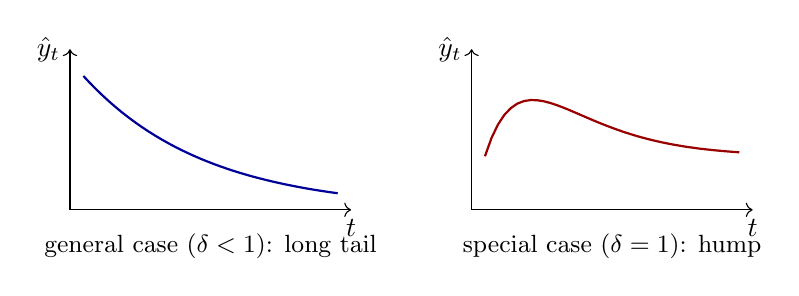
\begin{tikzpicture}[scale=0.85]
  \draw[->] (0,0)--(4.2,0) node[below]{$t$}; \draw[->] (0,0)--(0,2.4) node[left]{$\hat y_t$};
  \draw[thick,blue!60!black,domain=0.2:4,samples=40] plot(\x,{2*exp(-0.55*(\x-0.2))});
  \node at (2.1,-0.55){\small general case ($\delta<1$): long tail};
  \begin{scope}[xshift=6cm]
  \draw[->] (0,0)--(4.2,0) node[below]{$t$}; \draw[->] (0,0)--(0,2.4) node[left]{$\hat y_t$};
  \draw[thick,red!60!black,domain=0.2:4,samples=40] plot(\x,{0.8+3.2*(\x-0.2)*exp(-1.4*(\x-0.2))});
  \node at (2.1,-0.55){\small special case ($\delta=1$): hump};
  \end{scope}
\end{tikzpicture}
\end{center}
How to read the figure: each panel plots the response of (log) output to a one-time positive TFP shock, with time on the horizontal axis. In the general case output jumps on impact and then decays slowly, because the extra capital built during the boom wears out only gradually. In the $\delta=1$ case the AR(2) dynamics can produce a small hump, but the response dies out quickly because no capital survives from one period to the next.

\paragraph{Two solution methods.}
\begin{itemize}
  \item \textbf{Planner:} choose quantities directly to maximize welfare subject to the aggregate resource constraint, then recover prices from marginal products. No $w_t,r_t$ appear:
  \[
  \max_{\{c_t,l_t,k_{t+1}\}}E_0\sum_{t=0}^\infty\beta^t\big(\ln c_t+b\ln(1-l_t)\big)\quad\text{s.t.}\quad c_t+k_{t+1}=k_t^\alpha(A_tl_t)^{1-\alpha}+(1-\delta)k_t .
  \]
  \item \textbf{Decentralized:} given prices, solve the household and firm problems subject to their own constraints, then impose market clearing (which pins down prices).
  \item In the RBC model the two methods differ only in the constraint used (aggregate resource constraint vs.\ household budget constraint); there are no distortions, so by the welfare theorems they give the same allocation.
\end{itemize}

%=====================================================================
\subsection{General model ($\delta<1$): equilibrium system \pg{65}}

With $\delta<1$ there is no closed-form solution, so we (i) collect the equilibrium conditions, (ii) find the non-stochastic steady state, (iii) log-linearize around it, and (iv) solve the linear system.

\paragraph{Equilibrium.} Combine the resource constraint \eqref{eq:s6_kacc} with \eqref{eq:s6_prod}, the Euler equation \eqref{eq:s6_euler}, the interest rate from \eqref{eq:s6_prices}, and the labour condition \eqref{eq:s6_labour} with the firm's wage:
\begin{keybox}[title={Equilibrium system (unknowns $c_t,k_{t+1},l_t,r_t$; given $k_t$ and $A_t$)}]
\begin{align}
&c_t+k_{t+1}=(1-\delta)k_t+k_t^{\alpha}(A_tl_t)^{1-\alpha} \label{eq:s6_E1}\\
&\frac1{c_t}=\beta E_t\Big[\frac{1+r_{t+1}}{c_{t+1}}\Big]\label{eq:s6_E2}\\
&r_t=\alpha\Big(\frac{A_tl_t}{k_t}\Big)^{1-\alpha}-\delta\label{eq:s6_E3}\\
&(1-\alpha)\Big(\frac{k_t}{A_tl_t}\Big)^{\alpha}A_t=\frac{b\,c_t}{1-l_t}\label{eq:s6_E4}
\end{align}
plus the TFP process $\ln A_t=\rho_A\ln A_{t-1}+\varepsilon_{A,t}$ and the TVC.
\end{keybox}
Equation \eqref{eq:s6_E4} sets the wage paid by the firm equal to the wage required by the household ($w_t$ has been substituted out).

%=====================================================================
\subsection{Steady state \pg{66}}

In the non-stochastic steady state all shocks are zero, so $\ln A^*=0$, i.e.\ $A^*=1$, and every variable is constant: $x_t=x_{t+1}=x^*$. There is no uncertainty, so the expectation operator disappears. Equations \eqref{eq:s6_E1}--\eqref{eq:s6_E4} become
\begin{align*}
&\text{(a)}\quad c^*+k^*=k^{*\alpha}(A^*l^*)^{1-\alpha}+(1-\delta)k^*,\\
&\text{(b)}\quad \frac1{c^*}=\beta\frac{1+r^*}{c^*},\\
&\text{(c)}\quad r^*=\alpha\Big(\frac{A^*l^*}{k^*}\Big)^{1-\alpha}-\delta,\\
&\text{(d)}\quad w^*=\frac{b\,c^*}{1-l^*}=(1-\alpha)\Big(\frac{k^*}{A^*l^*}\Big)^{\alpha}A^*.
\end{align*}
Solve them in order, setting $A^*=1$.

\textbf{Step 1 (interest rate) from (b).} Multiply both sides by $c^*$:
\[
1=\beta(1+r^*)\quad\Rightarrow\quad r^*=\frac1\beta-1 .
\]
The steady-state interest rate is pinned down by impatience alone.

\textbf{Step 2 (capital--labour ratio) from (c).}
\begin{align*}
r^*+\delta&=\alpha\Big(\frac{l^*}{k^*}\Big)^{1-\alpha}\\
\Rightarrow\ \Big(\frac{k^*}{l^*}\Big)^{1-\alpha}&=\frac{\alpha}{r^*+\delta}\quad\text{(invert both sides)}\\
\Rightarrow\ \frac{k^*}{l^*}&=\Big(\frac{\alpha}{r^*+\delta}\Big)^{\frac1{1-\alpha}}.
\end{align*}

\textbf{Step 3 (ratios and wage).} With $y^*=k^{*\alpha}l^{*1-\alpha}$:
\begin{align*}
\frac{y^*}{k^*}&=\Big(\frac{k^*}{l^*}\Big)^{\alpha-1}=\frac{r^*+\delta}{\alpha}\quad\text{(from Step 2)},\\
w^*&=(1-\alpha)\Big(\frac{k^*}{l^*}\Big)^{\alpha}\quad\text{(from (d))}.
\end{align*}
From (a), the $k^*$ terms give $c^*=y^*-\delta k^*$ (investment just replaces depreciation, $i^*=\delta k^*$), so
\[
\frac{c^*}{k^*}=\frac{y^*}{k^*}-\delta=\frac{r^*+\delta}{\alpha}-\delta .
\]

\textbf{Step 4 (hours) from (d).} Write $c^*=\frac{c^*}{k^*}\cdot\frac{k^*}{l^*}\cdot l^*$ and substitute into $\frac{b\,c^*}{1-l^*}=(1-\alpha)\big(\frac{k^*}{l^*}\big)^{\alpha}$:
\begin{align*}
b\,\frac{c^*}{k^*}\,\frac{k^*}{l^*}\,\frac{l^*}{1-l^*}&=(1-\alpha)\Big(\frac{k^*}{l^*}\Big)^{\alpha}\\
\text{Divide by }\tfrac{k^*}{l^*}:\quad b\,\frac{c^*}{k^*}\,\frac{l^*}{1-l^*}&=(1-\alpha)\Big(\frac{k^*}{l^*}\Big)^{\alpha-1}=(1-\alpha)\frac{y^*}{k^*}\\
\Rightarrow\ \frac{l^*}{1-l^*}&=\frac{(1-\alpha)\,y^*/k^*}{b\,c^*/k^*}\\
\Rightarrow\ l^*&=\frac{(1-\alpha)\,y^*/k^*}{(1-\alpha)\,y^*/k^*+b\,c^*/k^*}\quad\Big(\text{using }\tfrac{l}{1-l}=z\iff l=\tfrac{z}{1+z}\Big).
\end{align*}

\textbf{Step 5 (levels).} $k^*=\frac{k^*}{l^*}\,l^*$, \ $y^*=\frac{y^*}{k^*}\,k^*$, \ $c^*=y^*-\delta k^*$, \ $i^*=\delta k^*$.

\begin{keybox}[title=Steady state of the RBC model]
\[
r^*=\tfrac1\beta-1,\quad \frac{k^*}{l^*}=\Big(\frac{\alpha}{r^*+\delta}\Big)^{\frac1{1-\alpha}},\quad
\frac{y^*}{k^*}=\frac{r^*+\delta}{\alpha},\quad \frac{c^*}{k^*}=\frac{r^*+\delta}{\alpha}-\delta,\quad
l^*=\frac{(1-\alpha)\,y^*/k^*}{(1-\alpha)\,y^*/k^*+b\,c^*/k^*}.
\]
\end{keybox}
Check: with $\delta=1$, $y^*/k^*=\frac{1}{\alpha\beta}$ and $c^*/k^*=\frac{1-\alpha\beta}{\alpha\beta}$, so $l^*=\frac{1-\alpha}{(1-\alpha)+b(1-\alpha\beta)}$, the same as the closed form. Interpretation: more patience ($\beta\uparrow$) lowers $r^*$, raises the capital--labour ratio and the wage; a stronger preference for leisure ($b\uparrow$) lowers $l^*$ but leaves all ratios unchanged.

%=====================================================================
\subsection{Log-linearization \pg{66}}

\paragraph{Definitions and approximation rules.} For any positive variable $x_t$ with steady state $x^*$, define the log-deviation
\[
\hat x_t\equiv\ln\frac{x_t}{x^*}\quad\Longleftrightarrow\quad x_t=x^*e^{\hat x_t}.
\]
$\hat x_t$ is approximately the percentage deviation of $x_t$ from steady state (e.g.\ $\hat x_t=0.01$: one percent above). We use the first-order Taylor approximation $e^{z}\approx1+z$ for small $z$, and drop all products of hatted variables (second-order terms). This gives three rules:
\begin{align*}
\text{(R1)}&\quad x_t=x^*e^{\hat x_t}\approx x^*(1+\hat x_t),\\
\text{(R2)}&\quad k_t^{a}l_t^{b}=(k^*e^{\hat k_t})^{a}(l^*e^{\hat l_t})^{b}=k^{*a}l^{*b}e^{a\hat k_t+b\hat l_t}\approx k^{*a}l^{*b}\big(1+a\hat k_t+b\hat l_t\big),\\
\text{(R3)}&\quad 1+r_t=1+r^*e^{\hat r_t}\approx(1+r^*)+r^*\hat r_t,\qquad 1-l_t\approx(1-l^*)-l^*\hat l_t .
\end{align*}
Since $A^*=1$, $\hat A_t=\ln A_t$ exactly, so the TFP process is already linear: $\hat A_t=\rho_A\hat A_{t-1}+\varepsilon_{A,t}$.

The recipe for each equation: substitute $x_t=x^*e^{\hat x_t}$, apply (R1)--(R3), then subtract the steady-state version of the equation so that only hatted terms remain.

\paragraph{Equation \eqref{eq:s6_E1}: resource constraint.} Apply (R1) to $c_t,k_{t+1},k_t$ and (R2) to output:
\[
c^*(1+\hat c_t)+k^*(1+\hat k_{t+1})=(1-\delta)k^*(1+\hat k_t)+k^{*\alpha}(A^*l^*)^{1-\alpha}\big[1+\alpha\hat k_t+(1-\alpha)(\hat A_t+\hat l_t)\big].
\]
Subtract the steady-state equation (a), $c^*+k^*=(1-\delta)k^*+y^*$ with $y^*=k^{*\alpha}(A^*l^*)^{1-\alpha}$:
\begin{equation}\label{eq:s6_L1}
c^*\hat c_t+k^*\hat k_{t+1}=(1-\delta)k^*\hat k_t+y^*\big[\alpha\hat k_t+(1-\alpha)(\hat A_t+\hat l_t)\big].
\end{equation}
Note that the left-hand capital term comes from $k_{t+1}$, so it carries $\hat k_{t+1}$. It is convenient to divide by $k^*$ and use $(1-\delta)+\alpha\frac{y^*}{k^*}=1-\delta+r^*+\delta=1+r^*=\frac1\beta$:
\begin{equation}\label{eq:s6_L1b}
\hat k_{t+1}=\frac1\beta\,\hat k_t+(1-\alpha)\frac{y^*}{k^*}\big(\hat A_t+\hat l_t\big)-\frac{c^*}{k^*}\,\hat c_t .
\end{equation}

\paragraph{Equation \eqref{eq:s6_E2}: Euler equation.} Left side: $\frac1{c_t}=\frac{1}{c^*}e^{-\hat c_t}\approx\frac1{c^*}(1-\hat c_t)$. Right side, using (R3) and (R1):
\begin{align*}
\beta E_t\Big[\frac{1+r_{t+1}}{c_{t+1}}\Big]
&\approx\beta E_t\Big[\big((1+r^*)+r^*\hat r_{t+1}\big)\frac{1}{c^*}(1-\hat c_{t+1})\Big]\\
\text{Factor out }(1+r^*):\quad&=\frac{\beta(1+r^*)}{c^*}E_t\Big[\Big(1+\frac{r^*}{1+r^*}\hat r_{t+1}\Big)(1-\hat c_{t+1})\Big]\\
\text{Use }\beta(1+r^*)=1,\ \tfrac{r^*}{1+r^*}=\beta r^*:\quad&=\frac1{c^*}E_t\big[(1+\beta r^*\hat r_{t+1})(1-\hat c_{t+1})\big]\\
\text{Drop the product of hats:}\quad&\approx\frac1{c^*}\big(1+\beta r^*E_t\hat r_{t+1}-E_t\hat c_{t+1}\big).
\end{align*}
Equate the two sides, multiply by $c^*$, and subtract 1:
\begin{align}
-\hat c_t&=\beta r^*E_t\hat r_{t+1}-E_t\hat c_{t+1}\notag\\
\Rightarrow\quad \hat c_t&=E_t\hat c_{t+1}-\beta r^*E_t\hat r_{t+1}. \label{eq:s6_L2}
\end{align}
Interpretation: a higher expected interest rate makes consumption today low relative to tomorrow (consumption grows faster).

\paragraph{Equation \eqref{eq:s6_E3}: interest rate.} Rewrite as $r_t+\delta=\alpha A_t^{1-\alpha}l_t^{1-\alpha}k_t^{-(1-\alpha)}$. Left side by (R3): $r^*+\delta+r^*\hat r_t$. Right side by (R2), and using (c), $\alpha(l^*/k^*)^{1-\alpha}=r^*+\delta$:
\[
r^*+\delta+r^*\hat r_t=(r^*+\delta)\big[1+(1-\alpha)(\hat A_t+\hat l_t-\hat k_t)\big].
\]
Subtract the steady state $r^*+\delta$:
\begin{equation}\label{eq:s6_L3}
r^*\hat r_t=(r^*+\delta)(1-\alpha)\big(\hat A_t+\hat l_t-\hat k_t\big).
\end{equation}
Interpretation: more TFP or more hours per unit of capital raise the marginal product of capital; more capital lowers it.

\paragraph{Equation \eqref{eq:s6_E4}: labour market.} Left side $=(1-\alpha)k_t^{\alpha}A_t^{1-\alpha}l_t^{-\alpha}$; by (R2) it is $\approx w^*\big(1+\alpha\hat k_t+(1-\alpha)\hat A_t-\alpha\hat l_t\big)$. For the right side, from (R3),
\[
1-l_t\approx(1-l^*)\Big(1-\frac{l^*}{1-l^*}\hat l_t\Big)
\ \Rightarrow\ \frac{1}{1-l_t}\approx\frac{1}{1-l^*}\Big(1+\frac{l^*}{1-l^*}\hat l_t\Big)\quad\Big(\text{using }\tfrac{1}{1-z}\approx1+z\Big),
\]
so $\frac{b\,c_t}{1-l_t}\approx\frac{b\,c^*}{1-l^*}\big(1+\hat c_t+\frac{l^*}{1-l^*}\hat l_t\big)=w^*\big(1+\hat c_t+\frac{l^*}{1-l^*}\hat l_t\big)$ by (d). Equate, divide by $w^*$, subtract 1:
\begin{equation}\label{eq:s6_L4}
\alpha\hat k_t+(1-\alpha)\hat A_t-\alpha\hat l_t=\hat c_t+\frac{l^*}{1-l^*}\,\hat l_t .
\end{equation}
The left side is the percentage change in the wage offered by firms ($\hat w_t$); the right side is the percentage change in the wage households require. For later use, the log-linear output is $\hat y_t=\alpha\hat k_t+(1-\alpha)(\hat A_t+\hat l_t)$ (by (R2) applied to \eqref{eq:s6_prod}).

\begin{keybox}[title=Log-linear RBC system]
\begin{align*}
\eqref{eq:s6_L1}&:\ c^*\hat c_t+k^*\hat k_{t+1}=(1-\delta)k^*\hat k_t+y^*\big[\alpha\hat k_t+(1-\alpha)(\hat A_t+\hat l_t)\big]\\
\eqref{eq:s6_L2}&:\ \hat c_t=E_t\hat c_{t+1}-\beta r^*E_t\hat r_{t+1}\\
\eqref{eq:s6_L3}&:\ r^*\hat r_t=(r^*+\delta)(1-\alpha)(\hat A_t+\hat l_t-\hat k_t)\\
\eqref{eq:s6_L4}&:\ \alpha\hat k_t+(1-\alpha)\hat A_t-\alpha\hat l_t=\hat c_t+\tfrac{l^*}{1-l^*}\hat l_t\\
&\phantom{:}\ \ \hat A_t=\rho_A\hat A_{t-1}+\varepsilon_{A,t}
\end{align*}
\end{keybox}

%=====================================================================
\subsection{Method of undetermined coefficients \pg{66}}

\paragraph{State variables and guess.} At date $t$ the state is $(\hat k_t,\hat A_t)$: $\hat k_t$ is endogenous but predetermined (chosen at $t-1$), $\hat A_t$ is exogenous. Everything else is a function of the state. Because the system is linear, guess linear policy rules with unknown coefficients $a_i,b_i$:
\begin{equation}\label{eq:s6_guess}
\hat c_t=a_1\hat k_t+b_1\hat A_t,\quad
\hat k_{t+1}=a_2\hat k_t+b_2\hat A_t,\quad
\hat l_t=a_3\hat k_t+b_3\hat A_t,\quad
\hat r_t=a_4\hat k_t+b_4\hat A_t .
\end{equation}
Once the $a_i,b_i$ are known, the whole path of $\hat c_t,\hat k_{t+1},\hat l_t,\hat r_t$ follows from any shock sequence.

\paragraph{Procedure.} Substitute \eqref{eq:s6_guess} into the log-linear system and require each equation to hold for \emph{all} values of $\hat k_t$ and $\hat A_t$; this means the coefficient on $\hat k_t$ and the coefficient on $\hat A_t$ must match separately. Define the shorthand $\eta\equiv\frac{l^*}{1-l^*}$ and $\theta\equiv\frac{(r^*+\delta)(1-\alpha)}{r^*}$.

\emph{From \eqref{eq:s6_L4}.} Collect $\hat l_t$: $(\alpha+\eta)\hat l_t=\alpha\hat k_t+(1-\alpha)\hat A_t-\hat c_t$. Substitute the guesses for $\hat l_t,\hat c_t$ and match:
\[
\hat k_t:\ a_3=\frac{\alpha-a_1}{\alpha+\eta},\qquad \hat A_t:\ b_3=\frac{1-\alpha-b_1}{\alpha+\eta}.
\]
\emph{From \eqref{eq:s6_L3}.} Divide by $r^*$: $\hat r_t=\theta(\hat A_t+\hat l_t-\hat k_t)$. Match:
\[
\hat k_t:\ a_4=\theta(a_3-1),\qquad \hat A_t:\ b_4=\theta(1+b_3).
\]
\emph{From \eqref{eq:s6_L1b}.} Substitute the guesses and match:
\[
\hat k_t:\ a_2=\frac1\beta+(1-\alpha)\frac{y^*}{k^*}a_3-\frac{c^*}{k^*}a_1,\qquad
\hat A_t:\ b_2=(1-\alpha)\frac{y^*}{k^*}(1+b_3)-\frac{c^*}{k^*}b_1 .
\]
\emph{From \eqref{eq:s6_L2}.} First compute the expectations. Since $\hat k_{t+1}$ is known at $t$ and $E_t\hat A_{t+1}=\rho_A\hat A_t$ (because $E_t\varepsilon_{A,t+1}=0$):
\begin{align*}
E_t\hat c_{t+1}&=a_1\hat k_{t+1}+b_1\rho_A\hat A_t=a_1(a_2\hat k_t+b_2\hat A_t)+b_1\rho_A\hat A_t,\\
E_t\hat r_{t+1}&=a_4(a_2\hat k_t+b_2\hat A_t)+b_4\rho_A\hat A_t .
\end{align*}
Substitute into $\hat c_t=E_t\hat c_{t+1}-\beta r^*E_t\hat r_{t+1}$ and match:
\begin{align*}
\hat k_t:&\quad a_1=a_1a_2-\beta r^*a_4a_2,\\
\hat A_t:&\quad b_1=a_1b_2+b_1\rho_A-\beta r^*\big(a_4b_2+b_4\rho_A\big).
\end{align*}

\paragraph{Solving.} Work in two blocks.
\begin{enumerate}
  \item \textbf{The $a$'s.} $a_3$, $a_4$, $a_2$ are linear in $a_1$ (from the first three ``$\hat k_t$'' conditions). Substituting them into $a_1=a_2(a_1-\beta r^*a_4)$ gives a \emph{quadratic} equation in $a_1$, hence two candidate solutions.
  \item \textbf{Pick the stable root.} One root gives $|a_2|<1$ (capital returns to steady state); the other gives $|a_2|>1$ (capital explodes). The explosive path violates the transversality condition $\lim_{T\to\infty}\beta^TE_0[\lambda_Tk_{T+1}]=0$ (capital would be accumulated forever and never consumed, or would hit zero), so we keep the root with $|a_2|<1$: $k_t$ cannot grow forever.
  \item \textbf{The $b$'s.} Given the $a$'s, the four ``$\hat A_t$'' conditions are \emph{linear} in $(b_1,b_2,b_3,b_4)$ and have a unique solution.
\end{enumerate}
For example, with $\alpha=0.33$, $\beta=0.99$, $\delta=0.025$, $b=2$, $\rho_A=0.95$ (quarterly), one finds $l^*\approx0.30$, $a_1\approx0.53$, $a_2\approx0.95$, $a_3\approx-0.27$, $b_1\approx0.28$, $b_2\approx0.08$, $b_3\approx0.50$. The other root of the quadratic gives $a_2\approx1.07>1$ and is discarded.

Interpretation: $a_2$ close to (but below) 1 means capital adjusts slowly back to steady state; this slow adjustment is the model's internal propagation mechanism. $b_3>0$ means hours rise after a positive TFP shock (unlike the $\delta=1$ case).

%=====================================================================
\subsection{Impulse response functions \pg{67}}

An \textbf{impulse response function} (IRF) traces the path of each variable after a single shock, with no further shocks, starting from steady state.

\paragraph{Procedure using the policy rules \eqref{eq:s6_guess}.}
\begin{itemize}
  \item $t=0$: the economy is in steady state, so all hatted variables are $0$: $\hat k_0=\hat A_0=0$.
  \item $t=1$: a one-time shock $\varepsilon_{A,1}>0$ hits; afterwards $\varepsilon_{A,t}=0$. From $\hat A_t=\rho_A\hat A_{t-1}+\varepsilon_{A,t}$: $\hat A_1=\varepsilon_{A,1}$, $\hat A_2=\rho_A\varepsilon_{A,1}$, and in general $\hat A_t=\rho_A^{\,t-1}\varepsilon_{A,1}$.
\end{itemize}
Period 1 (capital is predetermined, so it has not yet reacted):
\begin{align*}
\hat k_1&=a_2\hat k_0+b_2\hat A_0=0,\\
\hat c_1&=a_1\hat k_1+b_1\hat A_1=b_1\varepsilon_{A,1},\\
\hat l_1&=a_3\hat k_1+b_3\hat A_1=b_3\varepsilon_{A,1},\\
\hat r_1&=a_4\hat k_1+b_4\hat A_1=b_4\varepsilon_{A,1}.
\end{align*}
Period 2 and later: iterate forward,
\begin{align*}
\hat k_2&=a_2\hat k_1+b_2\hat A_1=b_2\varepsilon_{A,1},\qquad \hat c_2=a_1\hat k_2+b_1\rho_A\varepsilon_{A,1},\ \dots\\
\hat k_{t+1}&=a_2\hat k_t+b_2\hat A_t,\qquad \hat c_t=a_1\hat k_t+b_1\hat A_t,\qquad \hat l_t=a_3\hat k_t+b_3\hat A_t,
\end{align*}
and output follows from $\hat y_t=\alpha\hat k_t+(1-\alpha)(\hat A_t+\hat l_t)$.

\begin{center}
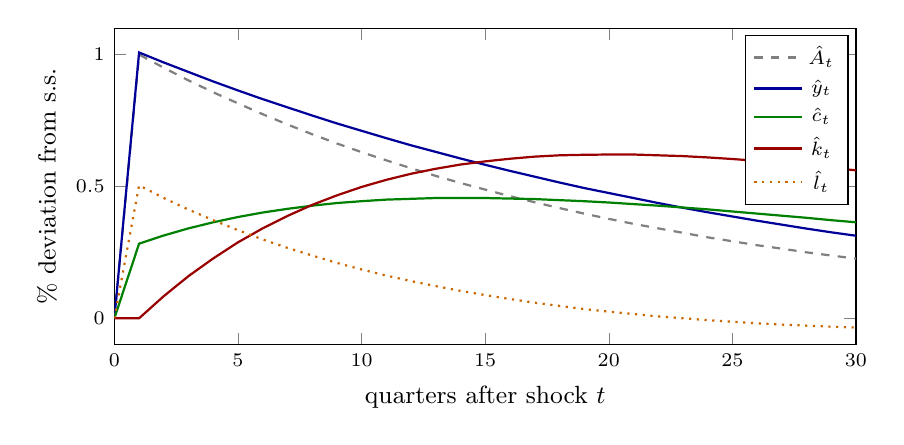
\begin{tikzpicture}
\begin{axis}[width=11cm,height=5.6cm,xmin=0,xmax=30,ymin=-0.1,ymax=1.1,
  xlabel={quarters after shock $t$},ylabel={\% deviation from s.s.},
  legend style={font=\scriptsize,at={(0.99,0.98)},anchor=north east},
  tick label style={font=\scriptsize},label style={font=\small}]
\addplot[thick,gray,dashed] coordinates {(0,0.000) (1,1.000) (2,0.950) (3,0.902) (4,0.857) (5,0.815) (6,0.774) (7,0.735) (8,0.698) (9,0.663) (10,0.630) (11,0.599) (12,0.569) (13,0.540) (14,0.513) (15,0.488) (16,0.463) (17,0.440) (18,0.418) (19,0.397) (20,0.377) (21,0.358) (22,0.341) (23,0.324) (24,0.307) (25,0.292) (26,0.277) (27,0.264) (28,0.250) (29,0.238) (30,0.226)};
\addlegendentry{$\hat A_t$}
\addplot[thick,blue!60!black] coordinates {(0,0.000) (1,1.008) (2,0.970) (3,0.934) (4,0.898) (5,0.864) (6,0.831) (7,0.800) (8,0.769) (9,0.739) (10,0.711) (11,0.683) (12,0.656) (13,0.631) (14,0.606) (15,0.582) (16,0.559) (17,0.537) (18,0.515) (19,0.494) (20,0.475) (21,0.456) (22,0.437) (23,0.419) (24,0.402) (25,0.386) (26,0.370) (27,0.355) (28,0.340) (29,0.326) (30,0.313)};
\addlegendentry{$\hat y_t$}
\addplot[thick,green!50!black] coordinates {(0,0.000) (1,0.283) (2,0.314) (3,0.341) (4,0.364) (5,0.384) (6,0.401) (7,0.415) (8,0.427) (9,0.437) (10,0.444) (11,0.450) (12,0.453) (13,0.456) (14,0.456) (15,0.456) (16,0.454) (17,0.452) (18,0.448) (19,0.444) (20,0.439) (21,0.433) (22,0.427) (23,0.420) (24,0.413) (25,0.405) (26,0.397) (27,0.389) (28,0.381) (29,0.372) (30,0.364)};
\addlegendentry{$\hat c_t$}
\addplot[thick,red!60!black] coordinates {(0,0.000) (1,0.000) (2,0.084) (3,0.160) (4,0.227) (5,0.288) (6,0.341) (7,0.388) (8,0.430) (9,0.466) (10,0.498) (11,0.525) (12,0.548) (13,0.567) (14,0.583) (15,0.595) (16,0.605) (17,0.613) (18,0.618) (19,0.620) (20,0.621) (21,0.621) (22,0.618) (23,0.615) (24,0.610) (25,0.604) (26,0.597) (27,0.589) (28,0.580) (29,0.571) (30,0.561)};
\addlegendentry{$\hat k_t$}
\addplot[thick,orange!80!black,dotted] coordinates {(0,0.000) (1,0.504) (2,0.456) (3,0.412) (4,0.372) (5,0.334) (6,0.299) (7,0.267) (8,0.238) (9,0.210) (10,0.185) (11,0.162) (12,0.141) (13,0.122) (14,0.104) (15,0.088) (16,0.073) (17,0.059) (18,0.047) (19,0.035) (20,0.025) (21,0.016) (22,0.007) (23,-0.000) (24,-0.007) (25,-0.013) (26,-0.019) (27,-0.024) (28,-0.028) (29,-0.032) (30,-0.035)};
\addlegendentry{$\hat l_t$}
\end{axis}
\end{tikzpicture}
\end{center}
How to read the figure: it plots the IRFs to a 1\% TFP shock at $t=1$, computed from the policy rules with the example parameters above. The horizontal axis is quarters after the shock; the vertical axis is the percent deviation from steady state. Output and hours jump on impact (output by more than TFP because hours rise); consumption rises by less and keeps rising (households smooth consumption, saving much of the windfall); capital is predetermined, so it starts at 0 and builds up slowly, peaking long after the shock. Because the extra capital wears off only slowly, output stays above steady state for many periods: the ``long tail'' of the general case.

%=====================================================================
\subsection{Frisch elasticity of labour supply \pg{67}}

\paragraph{Definition.} The \textbf{Frisch elasticity} is the elasticity of hours with respect to the wage, holding the marginal utility of wealth $\lambda_t$ (here $\lambda_t=1/c_t$) fixed:
\[
\varepsilon^{F}\equiv\frac{\partial\ln l_t}{\partial\ln w_t}\Big|_{\lambda_t\text{ fixed}}.
\]
Holding $\lambda_t$ fixed shuts down the income (wealth) effect, so the Frisch elasticity measures the pure \emph{intertemporal substitution} of labour: how willingly people shift work toward periods with temporarily high wages. Since temporary shocks barely change lifetime wealth, this is the elasticity that matters for business-cycle fluctuations in hours.

\paragraph{Case 1: separable power disutility.} Let $u=\ln c-\chi\frac{l^{1+\gamma}}{1+\gamma}$ with $\chi,\gamma>0$. The $[l_t]$ FOC (as in the Lagrangian above) is
\begin{align*}
\chi l_t^{\gamma}&=w_t\lambda_t\\
\text{Take logs:}\quad \ln\chi+\gamma\ln l_t&=\ln w_t+\ln\lambda_t\\
\text{Differentiate with }\lambda_t\text{ fixed:}\quad \gamma\,d\ln l_t&=d\ln w_t\\
\Rightarrow\quad \varepsilon^F&=\frac1\gamma .
\end{align*}

\paragraph{Case 2: the log-leisure utility of this section.} With $u=\ln c+b\ln(1-l)$ the FOC is $\frac{b}{1-l_t}=w_t\lambda_t$.
\begin{align*}
\text{Take logs:}\quad \ln b-\ln(1-l_t)&=\ln w_t+\ln\lambda_t\\
\text{Differentiate with }\lambda_t\text{ fixed:}\quad \frac{dl_t}{1-l_t}&=d\ln w_t\\
\text{Use }dl_t=l_t\,d\ln l_t:\quad \frac{l_t}{1-l_t}\,d\ln l_t&=d\ln w_t\\
\Rightarrow\quad \varepsilon^F&=\frac{1-l^*}{l^*}\quad\text{(evaluated at steady state)}.
\end{align*}
\begin{keybox}[title=Frisch elasticity]
\[
u=\ln c-\chi\tfrac{l^{1+\gamma}}{1+\gamma}:\ \ \varepsilon^F=\frac1\gamma;\qquad\qquad
u=\ln c+b\ln(1-l):\ \ \varepsilon^F=\frac{1-l^*}{l^*}\ \ (l^*=\tfrac13\Rightarrow\varepsilon^F=2).
\]
\end{keybox}
Interpretation: in the log-linear labour condition \eqref{eq:s6_L4}, the coefficient on $\hat l_t$ on the right is $\frac{l^*}{1-l^*}=1/\varepsilon^F$. A larger Frisch elasticity makes hours respond more strongly to wage movements, which helps the RBC model generate realistic fluctuations in hours. Micro estimates are usually much smaller (around $0.5$ or less), a well-known tension for the model.

\section{Monetary Policy: Rules vs Discretion (Barro-Gordon)}

\subsection{Rules vs discretion and the inflation bias \pg{88}}

\paragraph{Two ways to conduct policy.}
\begin{itemize}
  \item \textbf{Discretion:} policy is chosen \emph{period by period}. Each period the central bank (CB) picks the best action given the current situation, with no necessary connection between the choices made in different periods. In particular, it cannot bind its future self.
  \item \textbf{Rule:} the CB follows a \emph{formula} describing policy over a large number of periods, and commits to it in advance (before the public forms its expectations).
\end{itemize}

\begin{keybox}[title=Kydland--Prescott result]
Discretionary policymaking produces an \textbf{inflation bias}: the equilibrium inflation rate exceeds the socially desired inflation rate, without any gain in output.
\end{keybox}

\paragraph{Where does the bias come from?} Two ingredients are needed together.
\begin{enumerate}
  \item \textbf{The CB wants output above potential} (equivalently, unemployment below the natural rate).
  \begin{itemize}
    \item \emph{Potential output} is the highest output the economy can produce with resources fully used and without creating inflationary pressure.
    \item The \emph{natural rate of unemployment} is the unemployment rate in the market's long-run equilibrium.
    \item The CB is tempted to push output above potential by stimulating demand, e.g.\ by raising money growth.
  \end{itemize}
  \item \textbf{The CB cannot credibly commit to low inflation.} If firms and workers do not believe the CB will keep inflation low, they expect higher inflation and set wages and prices accordingly. Higher expected inflation then shows up as higher actual inflation.
\end{enumerate}
Interpretation: the public knows the CB is tempted to inflate, so it builds that inflation into its expectations in advance. The CB ends up delivering the expected (high) inflation simply to avoid an output loss, and output is no higher than it would have been with low inflation.

\subsection{AD--AS view of a monetary expansion \pg{88--89}}

\paragraph{Setup.}
\begin{itemize}
  \item $P$: price level; $y$: aggregate output; $y^*$: potential (natural) output.
  \item AD: aggregate demand curve, downward sloping in $(y,P)$. A monetary expansion shifts it to the right.
  \item SRAS: short-run aggregate supply, upward sloping because \emph{nominal} wages $w$ are fixed in the short run: a higher $P$ lowers the real wage $w/P$, so firms hire more labour $L$ and produce more.
  \item LRAS: long-run aggregate supply, vertical at $y^*$, since in the long run nominal wages fully adjust and the real wage returns to its market-clearing level.
\end{itemize}

\begin{center}
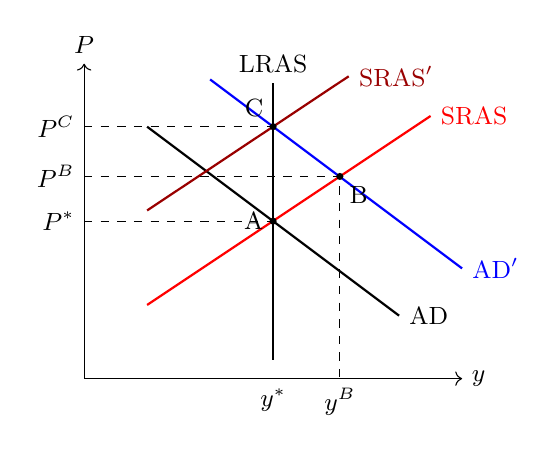
\begin{tikzpicture}[scale=0.8,font=\small]
  \draw[->] (0,0)--(6,0) node[right]{$y$};
  \draw[->] (0,0)--(0,5) node[above]{$P$};
  \draw[thick] (3,0.3)--(3,4.7) node[above]{LRAS};
  \draw[thick] (1,4)--(5,1) node[right]{AD};
  \draw[thick,blue] (2,4.75)--(6,1.75) node[right]{AD$'$};
  \draw[thick,red] (1,1.17)--(5.5,4.17) node[right]{SRAS};
  \draw[thick,red!60!black] (1,2.67)--(4.2,4.8) node[right]{SRAS$'$};
  \fill (3,2.5) circle (1.6pt) node[left]{A};
  \fill (4.06,3.21) circle (1.6pt) node[below right]{B};
  \fill (3,4) circle (1.6pt) node[above left]{C};
  \draw[dashed] (0,2.5) node[left]{$P^*$}--(3,2.5);
  \draw[dashed] (0,3.21) node[left]{$P^B$}--(4.06,3.21)--(4.06,0) node[below]{$y^B$};
  \draw[dashed] (0,4) node[left]{$P^C$}--(3,4);
  \node[below] at (3,0) {$y^*$};
\end{tikzpicture}
\end{center}
\emph{How to read the figure.} Output is on the horizontal axis and the price level on the vertical axis. The economy starts at A, where AD, SRAS and LRAS all cross. The expansion moves AD to the right (blue line), so the short-run equilibrium is B, on the old SRAS. Once nominal wages adjust, SRAS shifts up and to the left (dark red line), and the economy ends at C: back on LRAS, with a higher price level.

\paragraph{Step by step.}
\begin{itemize}
  \item \textbf{Initial equilibrium (A):} AD crosses SRAS on the LRAS line, at $(y^*,P^*)$. The economy is stable and no policy is changing.
  \item \textbf{Short run (A$\to$B):} the monetary expansion shifts AD to AD$'$, raising demand for goods and services. Along the old SRAS, with nominal wages fixed:
  \[
  P\uparrow\ \Rightarrow\ \frac{w}{P}\downarrow\ \Rightarrow\ \text{hiring is cheaper, } L\uparrow\ \Rightarrow\ y\uparrow .
  \]
  Price rises from $P^*$ to $P^B$ and output from $y^*$ to $y^B>y^*$.
  \item \textbf{Long run (B$\to$C):} over time workers see that the price level has risen and ask for higher nominal wages $w$ to protect their purchasing power. As $w$ rises, the real wage $w/P$ goes back to its original level. Labour costs rise, so SRAS shifts left to SRAS$'$:
  \[
  w\uparrow\ \Rightarrow\ \frac{w}{P}\uparrow \text{ (back to original)}\ \Rightarrow\ L\downarrow\ \Rightarrow\ y\downarrow \text{ back to } y^*,\qquad P\uparrow \text{ further to } P^C .
  \]
  \item \textbf{Outcome:} the price level is permanently higher ($P^C>P^B>P^*$), but output is back at potential $y^*$.
\end{itemize}
\begin{tipbox}
A demand shock (such as a monetary expansion) has real effects only when there is a market imperfection, here sticky nominal wages. Without such an imperfection, a demand shock only moves prices. In the long run: higher $P$, same $y^*$. This short-run real effect is exactly what tempts the CB in the Barro--Gordon model below.
\end{tipbox}

\subsection{Barro--Gordon model: setup \pg{89--91}}

\paragraph{Overview.} A static (one-period) model with a central bank and a private sector (workers and firms) that has rational expectations. The CB chooses money growth; the public chooses its inflation expectation (through nominal wage contracts) \emph{before} the CB acts.

\paragraph{Variables and parameters.}
\begin{itemize}
  \item $y$: actual output; $y_n$: natural (market-clearing) level of output.
  \item $\pi$: actual inflation rate; $\pi^e$: inflation rate expected by the public; $\bar\pi$: socially optimal inflation rate, assumed $\bar\pi=0$.
  \item $k>0$: political-pressure parameter. The CB's output target is $y_n+k$, i.e.\ \emph{above} the natural level.
  \item $\lambda>0$: weight the CB puts on output stabilization relative to price stabilization.
  \item $a>0$: sensitivity of output to inflation surprises $\pi-\pi^e$.
  \item $\Delta M$: growth rate of the money supply (the CB's instrument).
  \item $e$: supply shock; $v$: price (inflation) shock. Both have mean zero, are uncorrelated, and have variances $\sigma_e^2,\sigma_v^2$:
  \[
  E[e]=E[v]=0,\qquad E[ev]=E[e]E[v]=0,\qquad E[e^2]=\sigma_e^2,\qquad E[v^2]=\sigma_v^2 .
  \]
\end{itemize}

\paragraph{CB loss function.} The CB minimizes the expected value of
\begin{equation}
V=\tfrac12\lambda\,(y-y_n-k)^2+\tfrac12(\pi-\bar\pi)^2,\qquad \bar\pi=0 .\label{eq:bg-loss}
\end{equation}
The first term penalizes deviations of output from the target $y_n+k$; the second penalizes deviations of inflation from $0$. So the CB's problem is to stabilize $y$ around $y_n+k$ and $\pi$ around $0$.

\paragraph{Aggregate supply (expectations-augmented / Lucas supply).}
\begin{equation}
y=y_n+a(\pi-\pi^e)+e .\label{eq:bg-as}
\end{equation}
\begin{itemize}
  \item \textbf{Motivation:} wages are set in \emph{nominal} terms in one-period contracts, based on $\pi^e$. If actual inflation is higher than expected ($\pi>\pi^e$), prices rise faster than workers anticipated, the real wage is eroded, firms hire more workers and output rises above $y_n$. Only \emph{surprise} inflation raises output.
  \item $e$ is a supply shock that shifts aggregate supply left or right, e.g.\ a sharp rise in the price of a key input such as oil (a negative $e$).
\end{itemize}

\paragraph{Inflation.} The CB controls money growth but not inflation exactly:
\begin{equation}
\pi=\Delta M+v .\label{eq:bg-pi}
\end{equation}
The price shock $v$ means the CB cannot fully control $\pi$.

\paragraph{Timing of events.}
\begin{center}
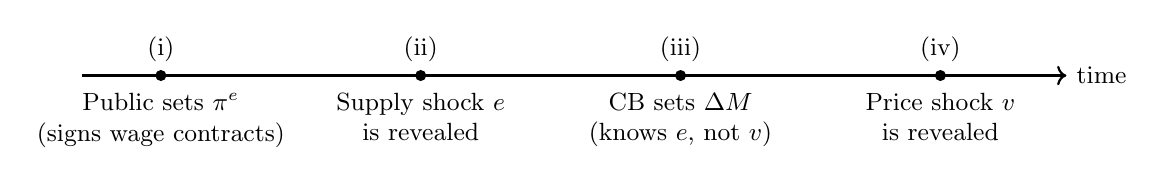
\begin{tikzpicture}[font=\small,x=1cm]
  \draw[->,thick] (0,0)--(12.5,0) node[right]{time};
  \foreach \x/\lab/\txt in {1/(i)/{Public sets $\pi^e$\\(signs wage contracts)},4.3/(ii)/{Supply shock $e$\\is revealed},7.6/(iii)/{CB sets $\Delta M$\\(knows $e$, not $v$)},10.9/(iv)/{Price shock $v$\\is revealed}}{
    \fill (\x,0) circle (2pt);
    \node[above] at (\x,0.05) {\lab};
    \node[below,align=center] at (\x,-0.1) {\txt};
  }
\end{tikzpicture}
\end{center}
Read the timeline left to right. Expectations are locked in first, so when the CB moves at stage (iii), $\pi^e$ is already fixed and the CB takes it as given. The CB can respond to $e$, which it has seen, but not to $v$, which is revealed only after it acts. So the public faces shocks and rigid wage contracts, and the CB uses monetary policy to stabilize output and inflation.

\paragraph{The loss in terms of the CB's instrument.} Substitute \eqref{eq:bg-as} into \eqref{eq:bg-loss}, using $\bar\pi=0$. Since $y-y_n=a(\pi-\pi^e)+e$,
\begin{equation}
V=\tfrac12\lambda\big[a(\pi-\pi^e)+e-k\big]^2+\tfrac12\pi^2 .\label{eq:bg-loss-pi}
\end{equation}
Now substitute $\pi=\Delta M+v$ from \eqref{eq:bg-pi} and expand $a(\pi-\pi^e)=a\Delta M+av-a\pi^e$:
\begin{equation}
V=\tfrac12\lambda\big[a\Delta M+av-a\pi^e+e-k\big]^2+\tfrac12(\Delta M+v)^2 .\label{eq:bg-loss-dm}
\end{equation}
How $\Delta M$ is chosen differs between discretion and a rule; that is the whole point of the comparison below.

\subsection{Equilibrium under discretion \pg{91--93}}

\paragraph{Solution strategy (backward induction).}
\begin{enumerate}
  \item Solve the CB's problem at stage (iii), taking $\pi^e$ and $e$ as given: this gives $\Delta M$ as a function of $(\pi^e,e)$.
  \item Go back to stage (i): the public, knowing this reaction function, forms rational expectations $\pi^e=E[\pi]$.
  \item Substitute $\pi^e$ back to get equilibrium $\Delta M$, $\pi$, output, and the expected loss.
\end{enumerate}

\paragraph{Step 1: the CB's problem.} Having observed $e$, and with $\pi^e$ already fixed, the CB solves
\[
\min_{\Delta M}\ E\{V\mid e\},
\]
where $V$ is \eqref{eq:bg-loss-dm} and the expectation is over the unknown $v$ only.

We use the chain rule, $\frac{d}{dx}\tfrac12 f(x)^2=f(x)f'(x)$, and the fact that we may differentiate inside the expectation. The derivative of the first term of \eqref{eq:bg-loss-dm} with respect to $\Delta M$ is $\lambda[\cdot]\cdot a$; the derivative of the second is $(\Delta M+v)$. The first-order condition (FOC) is
\begin{align*}
&E\big\{\lambda\big(a\Delta M+av-a\pi^e+e-k\big)a+\Delta M+v\ \big|\ e\big\}=0\\
\intertext{Multiply out the first term ($e$, $\pi^e$, $\Delta M$ are known, so only $v$ is random):}
&\lambda a^2\Delta M+\lambda a^2E[v]-\lambda a^2\pi^e+\lambda a e-\lambda a k+\Delta M+E[v]=0\\
\intertext{Use $E[v]=0$ and group the terms:}
&\lambda a^2\Delta M+\Delta M=\lambda a^2\pi^e+\lambda a(k-e)\\
\intertext{Factor out $\Delta M$:}
&(1+\lambda a^2)\,\Delta M=\lambda a^2\pi^e+\lambda a(k-e).
\end{align*}
The second-order condition holds since $\partial^2 V/\partial(\Delta M)^2=\lambda a^2+1>0$. Divide by $1+\lambda a^2$:
\begin{equation}
\Delta M=\frac{\lambda a^2\pi^e+\lambda a(k-e)}{1+\lambda a^2}.\label{eq:bg-dm}
\end{equation}
Interpretation of \eqref{eq:bg-dm}:
\begin{itemize}
  \item \textbf{Policy depends on the realized supply shock $e$.} A bad supply shock ($e<0$) lowers output and raises $\Delta M$ to offset it. Offsetting it fully would cost inflation, so the CB faces a \emph{trade-off} between stabilizing output and stabilizing inflation.
  \item \textbf{Optimal policy depends on $\pi^e$.} Higher expected inflation lowers output for a given $\pi$, so the CB partly accommodates it with more money growth.
\end{itemize}

\paragraph{The reaction function (special case $e=v=0$).} With no shocks, $\pi=\Delta M$ and \eqref{eq:bg-dm} becomes
\begin{equation}
\pi=\Delta M=\frac{\lambda a^2}{1+\lambda a^2}\,\pi^e+\frac{\lambda a}{1+\lambda a^2}\,k .\label{eq:bg-react}
\end{equation}
\begin{center}
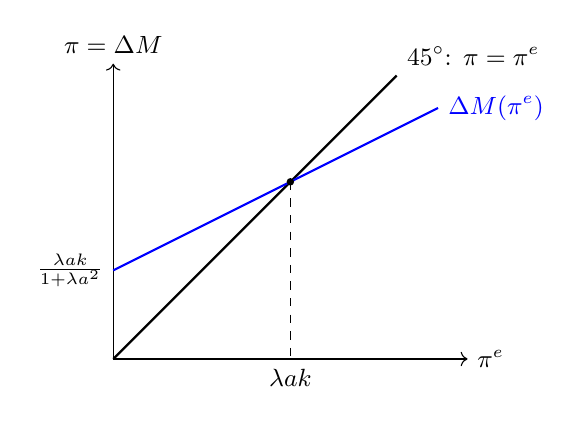
\begin{tikzpicture}[scale=0.75,font=\small]
  \draw[->] (0,0)--(6,0) node[right]{$\pi^e$};
  \draw[->] (0,0)--(0,5) node[above]{$\pi=\Delta M$};
  \draw[thick] (0,0)--(4.8,4.8) node[above right]{$45^\circ$: $\pi=\pi^e$};
  \draw[thick,blue] (0,1.5)--(5.5,4.25) node[right]{$\Delta M(\pi^e)$};
  \node[left] at (0,1.5) {$\frac{\lambda a k}{1+\lambda a^2}$};
  \fill (3,3) circle (1.8pt);
  \draw[dashed] (3,3)--(3,0) node[below]{$\lambda a k$};
\end{tikzpicture}
\end{center}
\emph{How to read the figure.} The horizontal axis is expected inflation and the vertical axis is the inflation the CB chooses. The blue line is the CB's best response \eqref{eq:bg-react}. Along the $45^\circ$ line, actual inflation equals expected inflation, which must hold in an equilibrium without shocks. The equilibrium is where the two lines cross.
\begin{itemize}
  \item \textbf{Intercept} $\frac{\lambda ak}{1+\lambda a^2}>0$ when $k>0$: even if the public expects zero inflation, the CB inflates.
  \item \textbf{Slope} $\frac{\lambda a^2}{1+\lambda a^2}<1$: the line is flatter than the $45^\circ$ line. The CB does not fully match an increase in expectations with money growth, because it also cares about inflation itself. The flatter the slope, the more weight it puts on inflation relative to output.
  \item \textbf{If $\pi^e=0$:} $\Delta M=\frac{\lambda a}{1+\lambda a^2}k$, which depends only on the political pressure $k$. If $k=0$, then $\Delta M=0$; if $k>0$, the CB raises $\Delta M$. So with $k>0$, $\pi^e=0$ \emph{cannot} be an equilibrium: the public would be surprised every time.
\end{itemize}

\paragraph{Step 2: rational expectations.} The public moves first and understands the CB's incentives, so it uses \eqref{eq:bg-dm} to form its expectation. It cannot predict $e$ or $v$, and both have mean zero. Rational expectations means $\pi^e=E[\pi]$:
\begin{align*}
\pi^e&=E[\pi]=E[\Delta M+v]=E[\Delta M] &&\text{(by \eqref{eq:bg-pi} and $E[v]=0$)}\\
&=\frac{\lambda a^2\pi^e+\lambda a(k-E[e])}{1+\lambda a^2} &&\text{(take expectations of \eqref{eq:bg-dm})}\\
&=\frac{\lambda a^2\pi^e+\lambda ak}{1+\lambda a^2} &&\text{(use $E[e]=0$).}
\end{align*}
Solve this for $\pi^e$. Multiply both sides by $1+\lambda a^2$:
\begin{align*}
(1+\lambda a^2)\pi^e&=\lambda a^2\pi^e+\lambda ak\\
\intertext{Subtract $\lambda a^2\pi^e$ from both sides:}
\pi^e&=\lambda ak .
\end{align*}
\begin{equation}
\boxed{\pi^e=\lambda ak>0}\label{eq:bg-pie}
\end{equation}
Expected inflation increases with $\lambda$ (more weight on output), with $a$ (surprises are more effective) and with $k$ (more ambitious output target). This is the crossing point in the figure: plugging $\pi^e=\lambda ak$ into \eqref{eq:bg-react} gives back $\pi=\lambda ak$.

\paragraph{Step 3: equilibrium money growth and inflation.} Substitute \eqref{eq:bg-pie} into \eqref{eq:bg-dm}:
\begin{align*}
\Delta M^D&=\frac{\lambda a^2(\lambda ak)+\lambda a(k-e)}{1+\lambda a^2}
=\frac{\lambda^2a^3k+\lambda ak-\lambda ae}{1+\lambda a^2}\\
\intertext{Factor $\lambda ak$ out of the first two terms of the numerator, $\lambda^2a^3k+\lambda ak=(1+\lambda a^2)\lambda ak$:}
&=\frac{(1+\lambda a^2)\lambda ak-\lambda ae}{1+\lambda a^2}
=\lambda ak-\frac{\lambda a}{1+\lambda a^2}\,e .
\end{align*}
Then by \eqref{eq:bg-pi}:
\begin{equation}
\Delta M^D=\lambda ak-\frac{\lambda a}{1+\lambda a^2}\,e,\qquad
\pi^D=\lambda ak-\frac{\lambda a}{1+\lambda a^2}\,e+v .\label{eq:bg-piD}
\end{equation}
Money growth has two parts. The constant $\lambda ak$ is the \emph{inflation bias}. The term $-\frac{\lambda a}{1+\lambda a^2}e$ is the stabilization response to the supply shock. Without $k$, policy would only stabilize the supply shock.

\paragraph{Output under discretion.} Compute the inflation surprise from \eqref{eq:bg-piD} and \eqref{eq:bg-pie}:
\[
\pi^D-\pi^e=-\frac{\lambda a}{1+\lambda a^2}\,e+v .
\]
Plug it into \eqref{eq:bg-as}:
\begin{align*}
y-y_n&=a(\pi-\pi^e)+e=-\frac{\lambda a^2}{1+\lambda a^2}\,e+av+e\\
\intertext{Combine the $e$ terms, $e-\frac{\lambda a^2}{1+\lambda a^2}e=\frac{1+\lambda a^2-\lambda a^2}{1+\lambda a^2}e$:}
y-y_n&=\frac{e}{1+\lambda a^2}+av .
\end{align*}
On average, output equals $y_n$: the bias buys \emph{no} extra output. Policy absorbs a fraction $\frac{\lambda a^2}{1+\lambda a^2}$ of the supply shock.

\paragraph{Expected loss under discretion, term by term.} Insert $y-y_n$ and $\pi^D$ into \eqref{eq:bg-loss-pi}:
\[
V=\frac{\lambda}{2}\Big[\underbrace{\frac{e}{1+\lambda a^2}+av-k}_{\text{output gap minus }k}\Big]^2
+\frac12\Big[\underbrace{\lambda ak-\frac{\lambda a}{1+\lambda a^2}\,e+v}_{\pi^D}\Big]^2 .
\]
Recall $(x+y+z)^2=x^2+y^2+z^2+2xy+2xz+2yz$. Expanding the first square:
\[
\Big[\tfrac{e}{1+\lambda a^2}+av-k\Big]^2=\frac{e^2}{(1+\lambda a^2)^2}+a^2v^2+k^2+\frac{2aev}{1+\lambda a^2}-\frac{2ke}{1+\lambda a^2}-2akv .
\]
Take expectations, using $E[e^2]=\sigma_e^2$, $E[v^2]=\sigma_v^2$, and $E[ev]=E[e]=E[v]=0$, so all cross terms vanish:
\[
E\Big[\tfrac{e}{1+\lambda a^2}+av-k\Big]^2=\frac{\sigma_e^2}{(1+\lambda a^2)^2}+a^2\sigma_v^2+k^2 .
\]
Expanding the second square in the same way:
\begin{multline*}
\Big[\lambda ak-\tfrac{\lambda a}{1+\lambda a^2}e+v\Big]^2=\lambda^2a^2k^2+\frac{\lambda^2a^2e^2}{(1+\lambda a^2)^2}+v^2\\
-\frac{2\lambda^2a^2ke}{1+\lambda a^2}+2\lambda akv-\frac{2\lambda aev}{1+\lambda a^2},
\end{multline*}
\[
E\Big[\lambda ak-\tfrac{\lambda a}{1+\lambda a^2}e+v\Big]^2=\lambda^2a^2k^2+\frac{\lambda^2a^2\sigma_e^2}{(1+\lambda a^2)^2}+\sigma_v^2 .
\]
Now assemble $E[V]=\frac{\lambda}{2}(\text{first})+\frac12(\text{second})$ and collect by $k^2$, $\sigma_v^2$, $\sigma_e^2$:
\begin{align*}
k^2\text{ terms:}\quad&\frac{\lambda}{2}k^2+\frac12\lambda^2a^2k^2=\frac{\lambda}{2}(1+\lambda a^2)k^2,\\
\sigma_v^2\text{ terms:}\quad&\frac{\lambda}{2}a^2\sigma_v^2+\frac12\sigma_v^2=\frac12(1+\lambda a^2)\sigma_v^2,\\
\sigma_e^2\text{ terms:}\quad&\frac{\lambda}{2}\frac{\sigma_e^2}{(1+\lambda a^2)^2}+\frac12\frac{\lambda^2a^2\sigma_e^2}{(1+\lambda a^2)^2}
=\frac{\lambda(1+\lambda a^2)\,\sigma_e^2}{2(1+\lambda a^2)^2}=\frac{\lambda}{2(1+\lambda a^2)}\sigma_e^2 .
\end{align*}
\begin{keybox}[title=Equilibrium under discretion]
\begin{equation}
\pi^e=\lambda ak,\qquad
V_D^e\equiv E[V]=\frac{\lambda}{2}(1+\lambda a^2)k^2+\frac12(1+\lambda a^2)\sigma_v^2+\frac{\lambda}{2(1+\lambda a^2)}\sigma_e^2 .\label{eq:bg-VD}
\end{equation}
\end{keybox}
The three terms are the cost of the political pressure $k$ (including the inflation bias), the cost of the uncontrollable price shock, and the cost of the supply shock after optimal stabilization.

\subsection{Equilibrium under a policy rule \pg{93--94}}

\paragraph{Setup.} The model equations \eqref{eq:bg-loss}--\eqref{eq:bg-pi} are unchanged. Now policy is a linear rule
\begin{equation}
\Delta M=b_0+b_1e ,\label{eq:bg-rule}
\end{equation}
where $b_0$ is the average money growth and $b_1$ is the response to the supply shock. Key difference from discretion:
\begin{itemize}
  \item The CB must commit to $b_0$ and $b_1$ \emph{before} the public forms $\pi^e$ and \emph{before} it observes $e$.
  \item So it chooses $b_0,b_1$ to minimize the \emph{unconditional} expected loss $E[V]$. Here $e$ is not given; it is random.
  \item Because the rule is announced first, the CB takes into account that its choice moves $\pi^e$.
\end{itemize}

\paragraph{Expected inflation under the rule.} From \eqref{eq:bg-pi} and \eqref{eq:bg-rule}, $\pi=b_0+b_1e+v$. With rational expectations and $E[e]=E[v]=0$:
\[
\pi^e=E[\pi]=b_0 .
\]
So the inflation surprise is $\pi-\pi^e=b_1e+v$, and $b_0$ drops out of it.

\paragraph{The CB's problem.} Substitute $\pi-\pi^e=b_1e+v$ and $\pi=b_0+b_1e+v$ into \eqref{eq:bg-loss-pi}:
\[
\min_{b_0,b_1}\ E\Big[\frac{\lambda}{2}\big(ab_1e+av+e-k\big)^2+\frac12\big(b_0+b_1e+v\big)^2\Big].
\]

\paragraph{FOC for $b_0$.} $b_0$ does not appear in the first square (it cancelled out of $\pi-\pi^e$), so only the second term contributes:
\begin{align*}
\frac{\partial E[V]}{\partial b_0}&=E\big[b_0+b_1e+v\big]=0\\
&\Rightarrow\ b_0+b_1E[e]+E[v]=0\ \Rightarrow\ b_0^*=0 .
\end{align*}
Under commitment, raising average money growth raises $\pi^e$ one for one, so it can never create an output surprise; it only adds inflation. The best average inflation is therefore zero.

\paragraph{FOC for $b_1$.} By the chain rule, $\partial(ab_1e+\dots)/\partial b_1=ae$ and $\partial(b_0+b_1e+v)/\partial b_1=e$:
\begin{align*}
\frac{\partial E[V]}{\partial b_1}&=E\Big[\lambda\big(ab_1e+av+e-k\big)ae+\big(b_0+b_1e+v\big)e\Big]=0\\
\intertext{Multiply out inside the expectation:}
&E\big[\lambda a^2b_1e^2+\lambda a^2ev+\lambda ae^2-\lambda ake+b_0e+b_1e^2+ev\big]=0\\
\intertext{Use $E[e^2]=\sigma_e^2$ and $E[ev]=E[e]=0$:}
&\lambda a^2b_1\sigma_e^2+0+\lambda a\sigma_e^2-0+0+b_1\sigma_e^2+0=0\\
\intertext{Divide by $\sigma_e^2>0$ and collect the $b_1$ terms:}
&(1+\lambda a^2)\,b_1=-\lambda a
\quad\Rightarrow\quad b_1^*=-\frac{\lambda a}{1+\lambda a^2}.
\end{align*}

\paragraph{Equilibrium under the rule.} Substituting $b_0^*,b_1^*$ into \eqref{eq:bg-rule}:
\begin{equation}
\Delta M^R=-\frac{\lambda a}{1+\lambda a^2}\,e,\qquad
\pi^R=-\frac{\lambda a}{1+\lambda a^2}\,e+v,\qquad
E[\pi^R]=\pi^e=0 .\label{eq:bg-piR}
\end{equation}
Expected inflation is zero. The response to the supply shock is \emph{the same} as under discretion.

\paragraph{Expected loss under the rule.} Output gap: $y-y_n=a(\pi-\pi^e)+e=-\frac{\lambda a^2}{1+\lambda a^2}e+av+e=\frac{e}{1+\lambda a^2}+av$, exactly as under discretion. Hence
\[
V=\frac{\lambda}{2}\Big[\frac{e}{1+\lambda a^2}+av-k\Big]^2+\frac12\Big[-\frac{\lambda a}{1+\lambda a^2}\,e+v\Big]^2 .
\]
The first expectation was already computed: $\frac{\sigma_e^2}{(1+\lambda a^2)^2}+a^2\sigma_v^2+k^2$. The second is the discretion one without the $\lambda ak$ term: $\frac{\lambda^2a^2\sigma_e^2}{(1+\lambda a^2)^2}+\sigma_v^2$. Collecting terms exactly as before (the only change is that the $\frac12\lambda^2a^2k^2$ term is gone):
\begin{keybox}[title=Equilibrium under the optimal rule]
\begin{equation}
\pi^e=0,\qquad
V_R^e=\frac{\lambda}{2}k^2+\frac12(1+\lambda a^2)\sigma_v^2+\frac{\lambda}{2(1+\lambda a^2)}\sigma_e^2 .\label{eq:bg-VR}
\end{equation}
\end{keybox}

\subsection{Comparing discretion and the rule \pg{94}}
Subtract \eqref{eq:bg-VR} from \eqref{eq:bg-VD}. The $\sigma_v^2$ and $\sigma_e^2$ terms are identical and cancel:
\begin{align*}
V_D^e-V_R^e&=\frac{\lambda}{2}(1+\lambda a^2)k^2-\frac{\lambda}{2}k^2
=\frac{\lambda}{2}k^2\big[(1+\lambda a^2)-1\big]
=\frac{\lambda^2a^2k^2}{2}>0 .
\end{align*}
\begin{keybox}[title=Rule beats discretion]
\[
V_D^e-V_R^e=\frac{\lambda^2a^2k^2}{2}>0 .
\]
The expected loss is lower under the rule. The gap is exactly the cost of the inflation bias, $\frac12(\lambda ak)^2$.
\end{keybox}

\paragraph{Why?} Compare output under the two regimes:
\begin{align*}
\text{Discretion:}\quad y-y_n&=a\Big(\lambda ak-\tfrac{\lambda a}{1+\lambda a^2}e+v-\lambda ak\Big)+e=\frac{e}{1+\lambda a^2}+av,\\
\text{Rule:}\quad y-y_n&=a\Big(0-\tfrac{\lambda a}{1+\lambda a^2}e+v-0\Big)+e=\frac{e}{1+\lambda a^2}+av .
\end{align*}
Output is \emph{identical}, and so is the response to shocks. The only difference is average inflation: $\lambda ak$ under discretion versus $0$ under the rule.
\begin{tipbox}
Under discretion the CB tries to exploit the short-run trade-off between inflation and output, because once $\pi^e$ is fixed, extra inflation seems to buy output. With rational expectations the public anticipates this, so $E[\pi]=\pi^e$ and there is no output gain, only higher inflation.
\begin{itemize}
  \item Discretion: $\pi$ high, $\pi^e$ high. Rule: $\pi$ low, $\pi^e$ low.
  \item In both cases the surprise is the same: $a(\pi-\pi^e)^D=a(\pi-\pi^e)^R$.
\end{itemize}
The rule wins because commitment lets the CB internalize that average money growth moves $\pi^e$ one for one.
\end{tipbox}

\subsection{Solutions to the inflation bias \pg{95}}

\paragraph{(1) Change the CB's mandate: a strict zero-inflation target, $\Delta M=0$.}
Suppose the CB is required to deliver $\pi=0$ on average and simply sets $\Delta M=0$, with no response to shocks. Then:
\begin{align*}
\pi&=v &&\text{(by \eqref{eq:bg-pi} with $\Delta M=0$)}\\
\pi^e&=E[\pi]=E[v]=0 &&\text{(rational expectations)}\\
y-y_n&=a(v-0)+e=av+e &&\text{(by \eqref{eq:bg-as}).}
\end{align*}
Expected loss, expanding $(av+e-k)^2=a^2v^2+e^2+k^2+2aev-2akv-2ke$ and dropping the cross terms, which have zero expectation:
\begin{align*}
V_0^e&=E\Big[\frac{\lambda}{2}(av+e-k)^2+\frac12v^2\Big]
=\frac{\lambda}{2}\big(a^2\sigma_v^2+\sigma_e^2+k^2\big)+\frac12\sigma_v^2\\
&=\frac{\lambda k^2}{2}+\frac12(1+\lambda a^2)\sigma_v^2+\frac{\lambda}{2}\sigma_e^2 .
\end{align*}
\emph{Compare with discretion.} Subtract term by term from \eqref{eq:bg-VD}:
\begin{align*}
V_D^e-V_0^e&=\Big[\frac{\lambda}{2}(1+\lambda a^2)k^2-\frac{\lambda}{2}k^2\Big]+\Big[\frac{\lambda}{2(1+\lambda a^2)}-\frac{\lambda}{2}\Big]\sigma_e^2\\
\intertext{Simplify each bracket, using $\frac{1}{1+\lambda a^2}-1=\frac{-\lambda a^2}{1+\lambda a^2}$:}
&=\frac{\lambda^2a^2k^2}{2}-\frac{\lambda^2a^2}{2(1+\lambda a^2)}\sigma_e^2\ \gtrless\ 0 .
\end{align*}
\begin{itemize}
  \item The first term is the \textbf{benefit} of $\Delta M=0$: the inflation bias disappears.
  \item The second term is its \textbf{cost}: the CB no longer stabilizes supply shocks.
  \item Discretion is preferred to $\Delta M=0$ ($V_D^e<V_0^e$) if and only if
  \[
  \frac{\lambda^2a^2k^2}{2}<\frac{\lambda^2a^2\sigma_e^2}{2(1+\lambda a^2)}
  \iff k^2<\frac{\sigma_e^2}{1+\lambda a^2},
  \]
  that is, when supply shocks are large relative to the bias, so flexibility is worth the extra inflation.
\end{itemize}
\emph{Compare with the rule.} Subtract $V_0^e$ from \eqref{eq:bg-VR}; the $k^2$ and $\sigma_v^2$ terms cancel:
\[
V_R^e-V_0^e=\Big[\frac{\lambda}{2(1+\lambda a^2)}-\frac{\lambda}{2}\Big]\sigma_e^2=-\frac{\lambda^2a^2}{2(1+\lambda a^2)}\sigma_e^2<0 .
\]
So the optimal rule is still the best. Even when $\Delta M=0$ beats discretion, it is only \emph{second best}: it removes the bias but gives up shock stabilization, while the optimal rule removes the bias \emph{and} keeps stabilization.

\paragraph{(2) Remove the political pressure $k$.} Compare the two policies:
\[
\Delta M^D=\lambda ak-\frac{\lambda a}{1+\lambda a^2}\,e,\qquad
\Delta M^R=-\frac{\lambda a}{1+\lambda a^2}\,e .
\]
With $k=0$ they coincide: discretion $=$ rule. If the CB has no desire to push output above its natural level (e.g.\ an independent CB without political pressure), it has nothing to gain from surprises, and the bias disappears.

\paragraph{(3) Reputation.} In a repeated setting, the CB can build a reputation for keeping inflation low. Suppose the public follows a \emph{trigger strategy}:
\[
\pi^e=\begin{cases}0 & \text{if the CB has so far kept } E[\Delta M]=0,\\[2pt] \lambda ak & \text{otherwise (the discretionary level, forever or for a punishment period).}\end{cases}
\]
Then $E[\Delta M]=0$ can be sustained as an equilibrium as long as the CB values its reputation enough. In each period the CB compares:
\begin{itemize}
  \item the \textbf{one-time gain} from cheating: with $\pi^e=0$ already set, it inflates to raise output;
  \item the \textbf{future cost}: the public then expects $\lambda ak$, and the CB suffers the discretionary loss instead of the rule loss, an extra $\frac{\lambda^2a^2k^2}{2}$ per period.
\end{itemize}
\emph{Illustration (no shocks, $e=v=0$).} If $\pi^e=0$ and the CB cheats, it plays its best response \eqref{eq:bg-react}, $\pi=\frac{\lambda ak}{1+\lambda a^2}$. Its loss is then $\frac{\lambda}{2}(a\pi-k)^2+\frac12\pi^2$, with $a\pi-k=-\frac{k}{1+\lambda a^2}$:
\[
\frac{\lambda}{2}\frac{k^2}{(1+\lambda a^2)^2}+\frac12\frac{\lambda^2a^2k^2}{(1+\lambda a^2)^2}=\frac{\lambda k^2}{2(1+\lambda a^2)} .
\]
Keeping $\pi=0$ gives loss $\frac{\lambda k^2}{2}$. So the gain from cheating is
\[
\frac{\lambda k^2}{2}-\frac{\lambda k^2}{2(1+\lambda a^2)}=\frac{\lambda^2a^2k^2}{2(1+\lambda a^2)} .
\]
This is smaller than the per-period punishment cost $\frac{\lambda^2a^2k^2}{2}$. With discount factor $\beta$ and a one-period punishment, low inflation is sustainable if $\frac{\lambda^2a^2k^2}{2(1+\lambda a^2)}\le\beta\frac{\lambda^2a^2k^2}{2}$, i.e.\ $\beta\ge\frac{1}{1+\lambda a^2}$. A longer punishment makes the condition easier to meet.

\begin{keybox}[title=Summary]
\begin{itemize}
  \item \textbf{Discretion:} $\pi^e=\lambda ak$, the same output as under the rule, and an extra expected loss $\frac12\lambda^2a^2k^2$ (the inflation bias).
  \item \textbf{Optimal rule (commitment):} $\Delta M=-\frac{\lambda a}{1+\lambda a^2}e$, $\pi^e=0$, the same shock response. This is the best regime.
  \item \textbf{Fixes for the bias:} commit to a rule; a zero-inflation mandate (removes the bias but not the stabilization cost, so second best at most); remove $k$; reputation (trigger strategies in repeated play).
\end{itemize}
\end{keybox}

\appendix
\section[Microeconomic Foundations: Competitive Markets, Welfare, Monopoly, Price Discrimination]{Microeconomic Foundations: Competitive Markets, Welfare,\\ Monopoly, Price Discrimination}

This appendix collects the partial-equilibrium microeconomics used throughout the notes: how a price-taking firm chooses output, how a market and an industry with free entry reach equilibrium, why competitive equilibrium maximizes total surplus, how taxes create deadweight loss, how a monopolist sets price, and how price discrimination changes output and welfare. Everything is static (one period) and, unless stated otherwise, goods are perfectly divisible.

\paragraph{Calculus facts used in this appendix.}
\begin{itemize}
\item \textbf{Chain rule:} if $y=y(p)$ then $\frac{d}{dp}f(y(p))=f'(y(p))\,y'(p)$.
\item \textbf{Implicit differentiation:} if an equation $G(p,m)=0$ defines $p$ as a function of $m$, differentiate both sides with respect to $m$ (treating $p=p(m)$) and solve for $p'(m)$.
\item \textbf{Comparative statics of an optimum:} if $y^*(c)$ solves $\max_y \pi(y,c)$, with FOC $\pi_y(y^*(c),c)=0$ and SOC $\pi_{yy}<0$, then differentiating the FOC in $c$ gives $\pi_{yy}\,\frac{dy^*}{dc}+\pi_{yc}=0$, i.e.\ $\frac{dy^*}{dc}=-\frac{\pi_{yc}}{\pi_{yy}}$.
\item \textbf{Concavity inequality:} a differentiable concave function lies below each of its tangent planes: $u(x')\le u(x^0)+\nabla u(x^0)\cdot(x'-x^0)$ for all $x',x^0$.
\item \textbf{Price elasticity of demand:} $\epsilon=\frac{dy}{dp}\frac{p}{y}$ (percentage change in quantity per 1\% change in price); $\epsilon<0$ for downward-sloping demand, and we write $|\epsilon|=-\epsilon$. Demand is \emph{elastic} if $|\epsilon|>1$, \emph{inelastic} if $|\epsilon|<1$.
\end{itemize}

%======================================================================
\subsection{The competitive firm and its supply curve \pg{45}}

\paragraph{Setup.}
\begin{itemize}
\item One good, produced in quantity $y\ge 0$ by a single firm.
\item $c(y)$: total cost of producing $y$. It splits as $c(y)=c_v(y)+F$, where $c_v(y)$ is variable cost (with $c_v(0)=0$) and $F\ge 0$ is a fixed cost that must be paid even if $y=0$ (short run).
\item Cost concepts: marginal cost $MC=c'(y)$; average cost $AC=c(y)/y$; average variable cost $AVC=c_v(y)/y$. Note $AC-AVC=F/y$.
\item $\bar p$: the market price. A \textbf{competitive firm} takes $\bar p$ as given and outside its control (it is a \emph{price-taker}).
\end{itemize}

Because consumers can buy from many other sellers at $\bar p$, the demand curve facing an ideal competitive firm is
\[
D(p)=\begin{cases}0 & \text{if } p>\bar p \quad(\text{no consumer pays more than the market price}),\\[2pt] \text{any amount} & \text{if } p=\bar p,\\[2pt] \infty & \text{if } p<\bar p \quad(\text{everyone would buy from this firm}).\end{cases}
\]
So the firm effectively sells any quantity it likes at $p=\bar p$; we write $p$ for that given price below.

\paragraph{Profit maximization.} The firm chooses $y$ to solve
\begin{equation}\label{eq:micro-cf}
\max_{y\ge 0}\ \pi(y)=p\,y-c(y).
\end{equation}
Differentiate with respect to $y$ and set to zero:
\begin{align*}
\pi'(y)&=p-c'(y)=0 &&\text{(first-order condition, FOC)}\\
\Longrightarrow\quad p&=c'(y^*). &&\text{(price = marginal cost)}
\end{align*}
The second-order condition (SOC) for a maximum is $\pi''(y^*)=-c''(y^*)\le 0$, i.e.\ $c''(y^*)\ge 0$: marginal cost must be non-decreasing at the optimum.

Read the FOC $p=c'(y)$ as a function of $y$: it gives the price at which the firm would want to supply $y$, the \textbf{inverse supply function} $p(y)=c'(y)$. Solving it for $y$ gives the supply function $y(p)$. The condition $p=MC$ is also what makes competitive output efficient (Section~\ref{sec:micro-welfare}): the price buyers pay equals the cost of the last unit.

\paragraph{1. The supply curve slopes up (interior solution).} The supply function satisfies the FOC identically in $p$:
\begin{align*}
p&=c'\big(y(p)\big) &&\text{for every } p\\
1&=c''\big(y(p)\big)\,y'(p) &&\text{(differentiate both sides w.r.t.\ $p$, chain rule)}\\
y'(p)&=\frac{1}{c''(y(p))}>0 &&\text{(divide by $c''>0$, the strict SOC).}
\end{align*}
\emph{Interpretation:} a higher price makes extra units worth producing even though each extra unit costs more (rising $MC$), so a competitive firm's supply curve has positive slope.

\paragraph{2. When is the interior solution chosen? (Shutdown condition.)} The firm can always choose $y=0$, in which case it pays only the fixed cost and earns $\pi(0)=-F$. Producing $y(p)>0$ is (weakly) better iff
\begin{align*}
p\,y(p)-c_v(y(p))-F&\ \ge\ -F &&\text{(profit from producing $\ge$ profit from shutting down)}\\
p\,y(p)-c_v(y(p))&\ \ge\ 0 &&\text{(add $F$ to both sides: $F$ is paid either way)}\\
p&\ \ge\ \frac{c_v(y(p))}{y(p)}=AVC(y(p)) &&\text{(divide by $y(p)>0$).}
\end{align*}
Combined with $p=MC$, the firm produces a positive amount only where $MC\ge AVC$.

\begin{keybox}[title=Short-run supply of a competitive firm]
\[
y(p)=\begin{cases}0 & \text{if } p<\min AVC,\\ \text{the solution of } p=c'(y) \text{ on the rising part of } MC & \text{if } p\ge \min AVC.\end{cases}
\]
The fixed cost $F$ does not affect the shutdown decision, because it is paid whether or not the firm produces.
\end{keybox}

\begin{center}
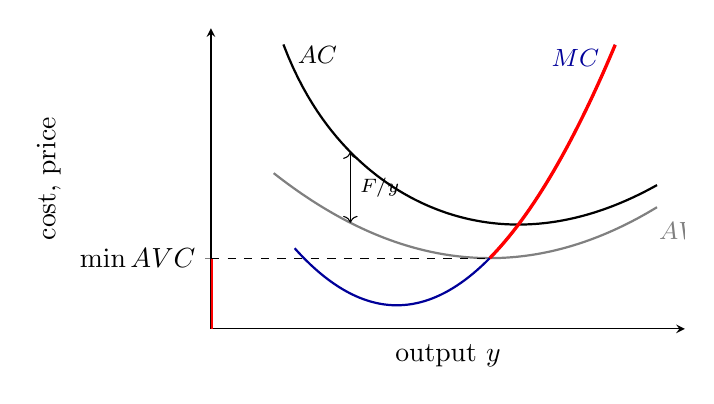
\begin{tikzpicture}
\begin{axis}[width=7.6cm,height=5.4cm,axis lines=left,xmin=0,xmax=3.4,ymin=0,ymax=8.5,
  xlabel={output $y$},ylabel={cost, price},xtick=\empty,ytick={2},yticklabels={$\min AVC$},
  domain=0.45:3.2,samples=80,restrict y to domain=0:8.3,clip=true]
\addplot[thick,black]{x^2-4*x+6+2/x} node[pos=0.04,right]{\small $AC$};
\addplot[thick,gray]{x^2-4*x+6} node[pos=0.97,below right]{\small $AVC$};
\addplot[thick,blue!60!black,domain=0.6:2.9]{3*x^2-8*x+6} node[pos=0.96,left]{\small $MC$};
\addplot[very thick,red,domain=2:2.9]{3*x^2-8*x+6};
\draw[very thick,red] (axis cs:0,0)--(axis cs:0,2);
\draw[dashed] (axis cs:0,2)--(axis cs:2,2);
\draw[<->,thin] (axis cs:1,3.0)--(axis cs:1,5.0) node[midway,right]{\scriptsize $F/y$};
\end{axis}
\end{tikzpicture}
\end{center}
\textit{How to read the figure.} Output is on the horizontal axis and cost per unit (or price) on the vertical axis. $AVC$ and $AC$ are U-shaped and $MC$ cuts both at their minima (when marginal cost is below an average, it pulls the average down; when above, it pulls it up). The vertical gap between $AC$ and $AVC$ is $F/y$, which shrinks as $y$ grows. The firm's supply curve is drawn in red: zero output (the vertical axis) for prices below $\min AVC$, and the $MC$ curve above its intersection with $AVC$.

%======================================================================
\subsection{Industry supply, market equilibrium, entry and exit \pg{46}}

\paragraph{Setup.}
\begin{itemize}
\item $n$ consumers, $i=1,\dots,n$, with individual demand functions $x_i(p)$; market demand $X(p)=\sum_{i=1}^n x_i(p)$, with $X'(p)<0$.
\item $m$ competitive firms, $j=1,\dots,m$, with supply functions $y_j(p)$ from the previous subsection, $y_j'(p)>0$.
\item \textbf{Industry supply} is the horizontal sum of firm supplies: $Y(p)=\sum_{j=1}^m y_j(p)$.
\end{itemize}

\paragraph{Market equilibrium.} The equilibrium price $p^*$ equates industry demand and industry supply:
\begin{equation}\label{eq:micro-mkteq}
\sum_{i=1}^{n} x_i(p^*)=\sum_{j=1}^{m} y_j(p^*).
\end{equation}

\paragraph{Effect of the number of firms on the price.} Let all $m$ firms be identical with supply $y(p)$, so industry supply is $m\,y(p)$ and \eqref{eq:micro-mkteq} becomes
\[
X(p)=m\,y(p).
\]
This equation defines the equilibrium price as an implicit function $p(m)$ of the number of firms. Differentiate both sides with respect to $m$ (product rule on the right, chain rule on both sides):
\begin{align*}
X'(p)\,p'(m)&=y(p)+m\,y'(p)\,p'(m) \\
X'(p)\,p'(m)-m\,y'(p)\,p'(m)&=y(p) &&\text{(collect the $p'(m)$ terms)}\\
p'(m)&=\frac{y(p)}{X'(p)-m\,y'(p)} &&\text{(divide by $X'(p)-m\,y'(p)$).}
\end{align*}
\emph{Sign:} the numerator $y(p)>0$; in the denominator $X'(p)<0$ and $-m\,y'(p)<0$, so the denominator is negative. Hence $p'(m)<0$. Each firm's output then changes by
\[
\frac{d\,y(p(m))}{dm}=y'(p)\,p'(m)<0 \qquad(\text{positive}\times\text{negative}).
\]
\emph{Interpretation:} more firms shift industry supply out, which lowers the market price, and each firm responds to the lower price by producing less ($m\uparrow\Rightarrow p\downarrow\Rightarrow y\downarrow$).

\paragraph{Entry and exit (long run).} In the long run the number of firms $m$ is variable. Assume there are no costs of entering or exiting and that potential entrants have the same cost function $c(y)$ as incumbents.
\begin{itemize}
\item If incumbents earn positive profit, new firms enter; each entrant adds its supply, so the industry supply curve becomes flatter and the price falls.
\item If firms make losses, some exit, and the price rises.
\item Entry stops when profit is zero: $p\,y-c(y)=0$, i.e.\ $p=AC(y)$. At the same time each firm sets $p=MC(y)$. Both hold only where $MC=AC$, which is the bottom of the $AC$ curve.
\end{itemize}

\begin{keybox}[title=Long-run competitive equilibrium with free entry]
\[
p^*=MC(y^*)=AC(y^*)=\min_y AC(y)\qquad(\text{break-even price}).
\]
When $m$ can be large, the long-run industry supply curve is (approximately) flat at $p^*$; demand determines only total quantity and hence the number of firms.
\end{keybox}

\paragraph{Example.} Let $c(y)=y^2+1$ (so $F=1$, $c_v(y)=y^2$). Then
\begin{align*}
AC(y)&=\frac{y^2+1}{y}=y+\frac1y, \qquad MC(y)=2y.\\
y+\frac1y&=2y &&\text{(break-even: set $AC=MC$)}\\
\frac1y&=y\ \Longrightarrow\ y^2=1\ \Longrightarrow\ y^*=1 &&\text{(subtract $y$; multiply by $y>0$)}\\
p^*&=MC(1)=2. &&\text{(and indeed $AC(1)=1+1=2$)}
\end{align*}
Each firm's supply is $y(p)=p/2$ (from $p=2y$), so with $m$ firms industry supply is $Y=m\,p/2$, i.e.\ the line $p=2Y/m$ through the origin, flatter for larger $m$. Firms keep entering as long as entry does not drive the equilibrium price below $2$. For instance, with market demand $p=8-Y$: $m=6$ firms give $8-Y=Y/3\Rightarrow Y=6$, $p=2$, each firm produces $1$ and earns zero profit; a seventh firm would push the price to $16/9<2$ and make every firm lose money.

\begin{center}
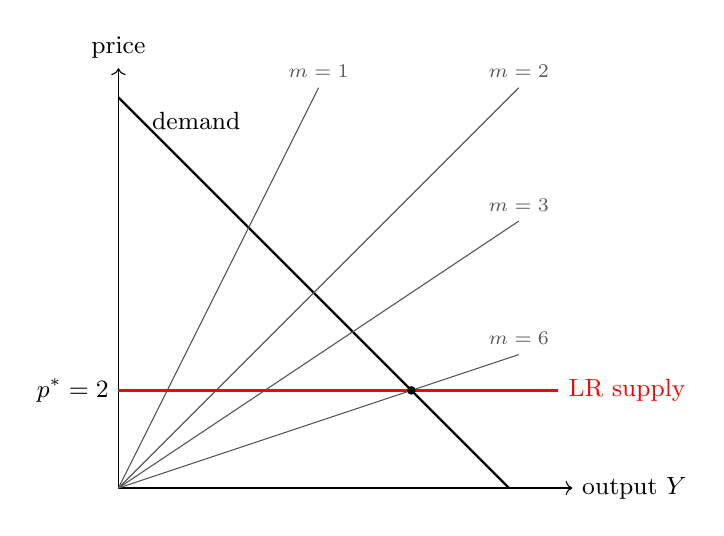
\begin{tikzpicture}[scale=0.62]
\draw[->] (0,0)--(9.3,0) node[right]{\small output $Y$};
\draw[->] (0,0)--(0,8.6) node[above]{\small price};
\draw[thick] (0,8)--(8,0) node[pos=0.06,right]{\small demand};
\foreach \m/\lab in {1/1,2/2,3/3,6/6}{
  \draw[gray!70!black] (0,0)--({min(8.2,4.1*\m)},{min(8.2,4.1*\m)*2/\m}) node[above,font=\scriptsize]{$m=\lab$};
}
\draw[very thick,red] (0,2)--(9,2) node[right]{\small LR supply};
\node[left] at (0,2) {\small $p^*=2$};
\fill (6,2) circle (2.5pt);
\end{tikzpicture}
\end{center}
\textit{How to read the figure.} Each grey ray is industry supply $p=2Y/m$ with $m$ firms; adding firms rotates it down (flatter). The demand line crosses successive rays at lower and lower prices. Entry continues until the crossing reaches the break-even price $p^*=2$ (here at $m=6$), so the long-run supply curve is the horizontal red line at $\min AC$.

%======================================================================
\subsection{Welfare: surplus and Pareto efficiency \pg{47--48}}\label{sec:micro-welfare}

\paragraph{Setup (one representative consumer).}
\begin{itemize}
\item Two goods: the $x$-good (the good being studied) and the $y$-good (``money'', all other goods), with the price of $y$ normalized to $1$.
\item \textbf{Quasilinear utility} $U(x,y)=u(x)+y$, with $u'>0$, $u''<0$, $u(0)=0$.
\item The consumer is endowed with $w$ units of the $y$-good. Producing $x$ units of the $x$-good uses up $c(x)$ units of the $y$-good ($c'>0$, $c''\ge 0$), so what is left to consume is $y=w-c(x)$.
\end{itemize}

\paragraph{The efficient quantity.} Choose $x$ to maximize utility:
\begin{align*}
&\max_{x,y}\ u(x)+y\quad\text{s.t.}\quad y=w-c(x)\\
\Longleftrightarrow\ &\max_x\ u(x)+w-c(x) &&\text{(substitute the constraint)}\\
\Longrightarrow\ & u'(x^*)=c'(x^*). &&\text{(FOC; $w$ is a constant)}
\end{align*}
The SOC $u''-c''<0$ holds by the assumptions.

\paragraph{Surplus interpretation.} With quasilinear utility, utility maximization at price $p$ gives $u'(x)=p$, so the inverse demand curve is the marginal-utility curve $u'(x)$; the competitive (inverse) supply curve is the marginal-cost curve $c'(x)$. Then, using $u(0)=0$:
\[
u(x)=\int_0^x u'(s)\,ds=\text{area under demand},\qquad c(x)-c(0)=\int_0^x c'(s)\,ds=\text{area under supply}.
\]
(Fixed costs $c(0)$ do not depend on $x$ and are ignored in what follows.) Define
\begin{align*}
CS(x)&=u(x)-p\,x &&\text{(consumer surplus: value minus amount paid)}\\
PS(x)&=p\,x-c(x) &&\text{(producer surplus = profit)}\\
CS(x)+PS(x)&=u(x)-p\,x+p\,x-c(x)=u(x)-c(x) &&\text{(payments $px$ cancel: a transfer).}
\end{align*}
So maximizing $u(x)-c(x)$ is the same as maximizing total surplus, the area under the demand curve and above the supply curve.

\begin{keybox}[title=First welfare result (partial equilibrium)]
In competitive equilibrium consumers set $u'(x)=p^*$ and firms set $c'(x)=p^*$, so $u'(x^*)=c'(x^*)$: the competitive output is exactly the one that maximizes total surplus $u(x)-c(x)$.
\end{keybox}

\begin{center}
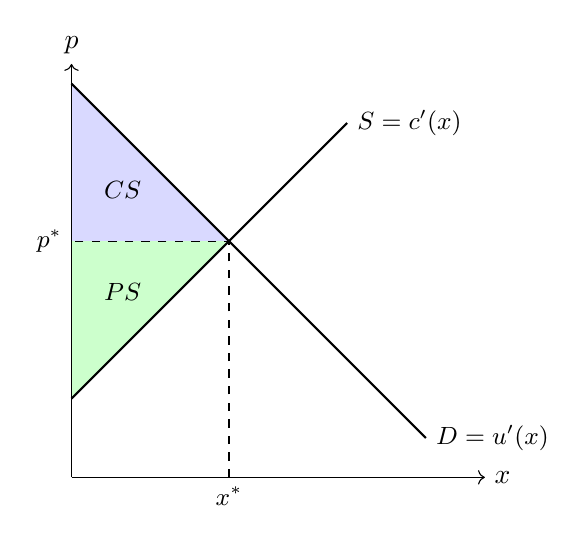
\begin{tikzpicture}[scale=0.5]
\fill[blue!15] (0,10)--(0,6)--(4,6)--cycle;
\fill[green!20] (0,6)--(0,2)--(4,6)--cycle;
\draw[->] (0,0)--(10.5,0) node[right]{$x$};
\draw[->] (0,0)--(0,10.5) node[above]{$p$};
\draw[thick] (0,10)--(9,1) node[right]{\small $D=u'(x)$};
\draw[thick] (0,2)--(7,9) node[right]{\small $S=c'(x)$};
\draw[dashed] (4,0) node[below]{\small $x^*$}--(4,6)--(0,6) node[left]{\small $p^*$};
\node at (1.3,7.3) {\small $CS$};
\node at (1.3,4.7) {\small $PS$};
\end{tikzpicture}
\end{center}
\textit{How to read the figure.} Demand slopes down because marginal utility diminishes; supply slopes up because marginal cost rises. Consumer surplus (blue) is the area between demand and the price line; producer surplus (green) is the area between the price line and supply. Their sum, the triangle between demand and supply up to $x^*$, is total surplus. Stopping at any $x<x^*$ would forgo units whose value $u'$ exceeds their cost $c'$; going beyond $x^*$ would produce units that cost more than they are worth.

\paragraph{Several consumers and firms.}
\begin{itemize}
\item Consumers $i=1,\dots,n$: utility $u_i(x_i)+y_i$, endowment $w_i$ of the $y$-good.
\item Firms $j=1,\dots,m$: firm $j$ produces $z_j$ units of the $x$-good at cost $c_j(z_j)$ (in units of the $y$-good).
\item Feasibility: total $x$ consumed equals total produced, $\sum_i x_i=\sum_j z_j$; total $y$ consumed equals endowments minus resources used in production, $\sum_{i=1}^n y_i=\sum_{i=1}^n w_i-\sum_{j=1}^m c_j(z_j)$.
\end{itemize}
A planner maximizes the sum of utilities $\sum_{i=1}^n u_i(x_i)+\sum_{i=1}^n y_i$. Substituting the $y$-feasibility condition:
\begin{equation}\label{eq:micro-planner}
\max_{\{x_i\},\{z_j\}}\ \sum_{i=1}^n u_i(x_i)+\sum_{i=1}^n w_i-\sum_{j=1}^m c_j(z_j)\quad\text{s.t.}\quad \sum_{i=1}^n x_i=\sum_{j=1}^m z_j .
\end{equation}
Lagrangian with multiplier $\lambda$ on the constraint:
\[
\mathcal L=\sum_i u_i(x_i)+\sum_i w_i-\sum_j c_j(z_j)+\lambda\Big(\sum_j z_j-\sum_i x_i\Big).
\]
FOCs:
\begin{align*}
\frac{\partial\mathcal L}{\partial x_i}&=u_i'(x_i^*)-\lambda=0\ \Longrightarrow\ u_i'(x_i^*)=\lambda\quad\text{for all } i,\\
\frac{\partial\mathcal L}{\partial z_j}&=-c_j'(z_j^*)+\lambda=0\ \Longrightarrow\ c_j'(z_j^*)=\lambda\quad\text{for all } j.
\end{align*}
These are exactly the competitive equilibrium conditions with $p^*=\lambda$: each consumer sets $u_i'(x_i)=p^*$, each firm sets $c_j'(z_j)=p^*$. \emph{Interpretation:} the equilibrium price acts as the shadow value of the $x$-good, equating every consumer's marginal utility with every firm's marginal cost, which is what the planner wants.

\paragraph{Pareto efficiency.} A more general welfare criterion than ``sum of utilities'' is Pareto efficiency.
\begin{itemize}
\item An allocation is \textbf{Pareto efficient} if there is no other feasible allocation that makes some agent better off without making any agent worse off.
\end{itemize}
To characterize it, take two agents and total resources $\bar x$, $\bar y$ (so $x_2=\bar x-x_1$, $y_2=\bar y-y_1$). An allocation is Pareto efficient iff it maximizes agent 1's utility holding agent 2's utility at some level $\bar u$:
\begin{align*}
&\max_{x_1,y_1}\ u_1(x_1)+y_1\quad\text{s.t.}\quad u_2(\bar x-x_1)+\bar y-y_1=\bar u\\
&y_1=u_2(\bar x-x_1)+\bar y-\bar u &&\text{(solve the constraint for $y_1$)}\\
&\max_{x_1}\ u_1(x_1)+u_2(\bar x-x_1)+(\bar y-\bar u) &&\text{(substitute; $\bar y-\bar u$ is a constant)}\\
&u_1'(x_1)-u_2'(\bar x-x_1)=0 &&\text{(FOC, chain rule on $u_2$)}.
\end{align*}
\begin{keybox}[title=Necessary condition for Pareto efficiency (quasilinear case)]
\[
u_1'(x_1)=u_2'(x_2),\qquad x_2=\bar x-x_1:
\]
marginal utilities of the $x$-good (in units of money) are equalized across agents. So, essentially, Pareto efficiency requires maximizing $u_1(x_1)+u_2(x_2)$.
\end{keybox}
\emph{Interpretation:} if agent 1's marginal utility were higher, moving a little $x$ from agent 2 to agent 1, and having agent 1 hand agent 2 just enough $y$ to compensate, would leave agent 2 indifferent and agent 1 strictly better off. In competitive equilibrium every consumer sets $u_i'(x_i)=p^*$, so the marginal utilities are automatically equal and the equilibrium is Pareto efficient.

\begin{tipbox}
With quasilinear utility, the way the $y$-good (``money'') is divided does not affect efficiency: the efficiency condition pins down only the allocation of $x$. Moving $y$ between people is pure redistribution: it changes fairness (equity), not efficiency.
\end{tipbox}

%======================================================================
\subsection{Taxes and subsidies \pg{49}}

\paragraph{Setup.} A tax drives a wedge between two prices:
\begin{itemize}
\item $p_d$: the \textbf{demand price}, paid by buyers (including the tax);
\item $p_s$: the \textbf{supply price}, received by sellers.
\end{itemize}
The demand function is $D(\cdot)$ and supply function $S(\cdot)$; $P_d(x)$ and $P_s(x)$ are the inverse demand and inverse supply curves. Three instruments:
\begin{itemize}
\item \textbf{Quantity (unit) tax} $t$ per unit sold: $p_d=p_s+t$.
\item \textbf{Value (ad valorem) tax} at rate $\tau$ on expenditure: $p_d=(1+\tau)\,p_s$.
\item \textbf{Quantity subsidy} $s$ per unit: the seller receives $s$ more per unit than the buyer pays, so $p_d=p_s-s$.
\end{itemize}

\paragraph{Equilibrium.} Buyers respond to $p_d$, sellers to $p_s$, and quantity demanded must equal quantity supplied:
\[
D(p_d)=S(p_s),\qquad p_d=p_s+t .
\]
Equivalently, with inverse curves, the equilibrium quantity $x_t$ solves
\[
P_d(x_t)=P_s(x_t)+t\qquad\big(\text{or } P_s(x_t)=P_d(x_t)-t\big),
\]
and then $p_d=P_d(x_t)$, $p_s=P_s(x_t)$. Since $P_d$ falls and $P_s$ rises in $x$, a positive $t$ requires a smaller $x$: $x_t<x^*$, where $x^*$ is the no-tax quantity ($P_d(x^*)=P_s(x^*)$).

\paragraph{Welfare with the tax.} At the post-tax quantity $x_t$ (with $u$ and $c$ as in Section~\ref{sec:micro-welfare}):
\begin{align*}
CS&=u(x_t)-p_d\,x_t &&\text{(buyers pay $p_d$)}\\
PS&=p_s\,x_t-c(x_t) &&\text{(sellers receive $p_s$)}\\
T&=t\,x_t=(p_d-p_s)\,x_t &&\text{(tax revenue, returned to society)}\\
W(x_t)=CS+PS+T&=u(x_t)-p_dx_t+p_sx_t-c(x_t)+(p_d-p_s)x_t\\
&=u(x_t)-c(x_t). &&\text{(all payments cancel)}
\end{align*}
Tax revenue must be counted as part of welfare: it is a transfer from buyers and sellers to the government, not a loss.

\begin{keybox}[title=Deadweight loss]
\[
DWL=W(x^*)-W(x_t)=\int_{x_t}^{x^*}\big[u'(s)-c'(s)\big]\,ds>0 .
\]
It is the surplus from the trades between $x_t$ and $x^*$ that no longer happen, although buyers valued those units above their cost of production.
\end{keybox}

\begin{center}
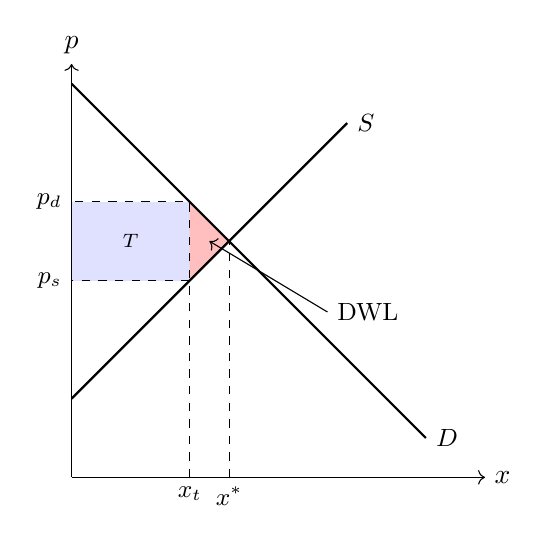
\begin{tikzpicture}[scale=0.5]
\fill[blue!12] (0,5) rectangle (3,7);
\fill[red!25] (3,7)--(3,5)--(4,6)--cycle;
\draw[->] (0,0)--(10.5,0) node[right]{$x$};
\draw[->] (0,0)--(0,10.5) node[above]{$p$};
\draw[thick] (0,10)--(9,1) node[right]{\small $D$};
\draw[thick] (0,2)--(7,9) node[right]{\small $S$};
\draw[dashed] (3,0) node[below]{\small $x_t$}--(3,7)--(0,7) node[left]{\small $p_d$};
\draw[dashed] (3,5)--(0,5) node[left]{\small $p_s$};
\draw[dashed] (4,0) node[below]{\small $x^*$}--(4,6);
\node at (1.5,6) {\scriptsize $T$};
\draw[<-] (3.5,6)--(6.5,4.2) node[right]{\small DWL};
\end{tikzpicture}
\end{center}
\textit{How to read the figure.} Without the tax the market clears at $x^*$. With a unit tax $t$, the quantity $x_t$ is where the vertical gap between demand and supply equals $t$: buyers pay $p_d$, sellers get $p_s=p_d-t$. The blue rectangle (height $t$, width $x_t$) is tax revenue $T$, a transfer. The red triangle between $x_t$ and $x^*$ is the deadweight loss: surplus that nobody receives.

%======================================================================
\subsection{Monopoly: the pricing rule \pg{50--52}}

\paragraph{Setup.}
\begin{itemize}
\item A single seller (the \textbf{monopolist}) with cost function $c(y)$, $c'>0$.
\item Market demand $D(p)$, downward sloping; its inverse $p(y)$ (the price at which consumers buy exactly $y$) satisfies $p'(y)<0$.
\item Revenue $r(y)=p(y)\,y$; marginal revenue $MR=r'(y)$.
\end{itemize}
A monopolist has market power: the amount it can sell responds \emph{continuously} to the price it charges. Contrast the competitive firm, whose sales drop to zero if it charges above the market price. A competitive firm is a price-taker; a monopolist is a \textbf{price-maker}.

\paragraph{The problem.} The monopolist faces two constraints, technology ($c(y)$) and consumer behaviour (it cannot sell more than is demanded):
\[
\max_{p,\,y}\ p\,y-c(y)\quad\text{s.t.}\quad D(p)\ge y .
\]
It would never produce output it cannot sell, so the constraint binds, $y=D(p)$. The problem can be written in terms of price, $\max_p\ p\,D(p)-c(D(p))$, or, more conveniently, using the inverse demand curve, in terms of quantity:
\begin{equation}\label{eq:micro-monop}
\max_y\ \pi(y)=p(y)\,y-c(y).
\end{equation}
Differentiate (product rule on $p(y)\,y$):
\begin{align}
\text{FOC:}\quad & \underbrace{p(y)+p'(y)\,y}_{MR=r'(y)}=\underbrace{c'(y)}_{MC}, \label{eq:micro-mrmc}\\
\text{SOC:}\quad & \pi''(y)=2p'(y)+p''(y)\,y-c''(y)\le 0. \notag
\end{align}

\paragraph{Why marginal revenue is below price.} When the monopolist considers selling $dy$ more units there are two effects:
\begin{itemize}
\item revenue rises by $p\,dy$ from selling the extra units at the current price;
\item but to sell them it must cut the price by $dp=p'(y)\,dy<0$ on all $y$ units it already sells.
\end{itemize}
So $dr=p\,dy+y\,dp=\big[p+p'(y)\,y\big]\,dy$. Since $p'(y)<0$, $MR<p(y)$ for every $y>0$, while at $y=0$, $MR=p(0)$: the first unit costs no price cut on earlier units. Hence the $MR$ curve starts at the demand intercept and lies below the inverse demand curve.

The SOC says that the slope of $MR$, $2p'+p''y$, is less than the slope of $MC$, $c''$: the $MR$ curve cuts the $MC$ curve \emph{from above}.

\paragraph{Elasticity form of the FOC.} Factor $p(y)$ out of $MR$:
\begin{align*}
r'(y)&=p(y)\Big[1+\frac{dp}{dy}\,\frac{y}{p}\Big] &&\text{(factor out $p$)}\\
&=p(y)\Big[1+\frac{1}{\epsilon(y)}\Big], &&\epsilon(y)=\frac{p}{y}\frac{dy}{dp}\ \text{(so }\tfrac{dp}{dy}\tfrac{y}{p}=\tfrac{1}{\epsilon}\text{)}\\
&=p(y)\Big[1-\frac{1}{|\epsilon(y)|}\Big] &&\text{(since $\epsilon<0$, $\epsilon=-|\epsilon|$).}
\end{align*}
So the FOC \eqref{eq:micro-mrmc} reads
\begin{equation}\label{eq:micro-markup}
p(y)\Big[1-\frac{1}{|\epsilon(y)|}\Big]=c'(y).
\end{equation}
\emph{Demand must be elastic at the optimum.} If $|\epsilon(y)|<1$, the bracket is negative, so $MR<0<MC$: cutting output would raise revenue \emph{and} lower cost. Hence at the monopoly optimum $|\epsilon(y)|\ge 1$ (strictly $>1$ when $MC>0$), i.e.\ $\epsilon(y)<-1$.

\begin{keybox}[title=Monopoly markup rule]
Solving \eqref{eq:micro-markup} for $p$:
\[
p=\frac{c'(y)}{1-1/|\epsilon|}.
\]
Price is a markup over marginal cost; the markup is larger the less elastic is demand, and goes to zero (price $\to MC$) as $|\epsilon|\to\infty$, the competitive case.
\end{keybox}

\paragraph{Special case 1: linear demand.} Let $p(y)=a-by$ ($a,b>0$) and constant marginal cost, $c(y)=cy$ with $c<a$.
\begin{align*}
r(y)&=ay-by^2,\qquad r'(y)=a-2by &&\text{($MR$ is twice as steep as demand)}\\
a-2by^*&=c &&\text{(set $MR=MC$)}\\
y^*&=\frac{a-c}{2b} &&\text{(solve for $y$)}\\
p^*&=a-b\,\frac{a-c}{2b}=\frac{a+c}{2}. &&\text{(substitute into demand)}
\end{align*}
For comparison, the competitive outcome $p=c$ gives $y_c=(a-c)/b=2y^*$: the monopolist produces half the competitive output.

\paragraph{Special case 2: constant-elasticity demand.} Let $y=A\,p^{-b}$ with $A>0$, $b>1$. Then
\[
\epsilon=\frac{p}{y}\frac{dy}{dp}=\frac{p}{Ap^{-b}}\cdot(-b)A\,p^{-b-1}=-b,
\]
constant at every point. With constant marginal cost $c$, \eqref{eq:micro-markup} gives
\[
p=\frac{c}{1-1/b}=\frac{b}{b-1}\,c,
\]
a \emph{constant} markup over marginal cost whose size depends only on the elasticity of demand.

\begin{center}
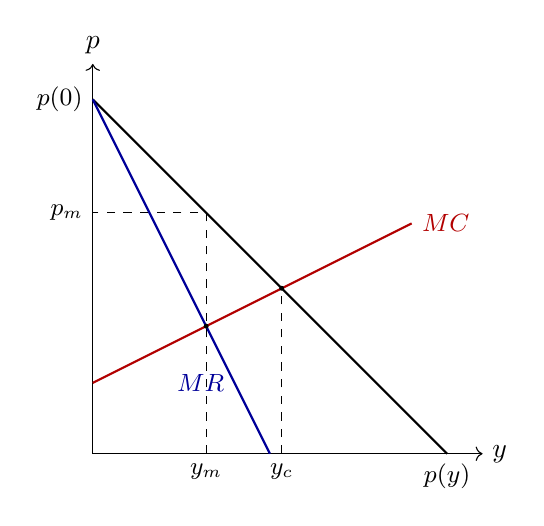
\begin{tikzpicture}[scale=0.45]
\draw[->] (0,0)--(11,0) node[right]{$y$};
\draw[->] (0,0)--(0,11) node[above]{$p$};
\draw[thick] (0,10) node[left]{\small $p(0)$}--(10,0) node[below]{\small $p(y)$};
\draw[thick,blue!60!black] (0,10)--(5,0) node[pos=0.8,left]{\small $MR$};
\draw[thick,red!70!black] (0,2)--(9,6.5) node[right]{\small $MC$};
\draw[dashed] (3.2,0) node[below]{\small $y_m$}--(3.2,6.8)--(0,6.8) node[left]{\small $p_m$};
\draw[dashed] (5.33,0) node[below]{\small $y_c$}--(5.33,4.67);
\fill (3.2,3.6) circle (2pt);
\fill (5.33,4.67) circle (2pt);
\end{tikzpicture}
\end{center}
\textit{How to read the figure.} Inverse demand $p(y)$ is the consumers' marginal willingness to pay; $MR$ starts at the same intercept $p(0)$ and falls twice as fast (linear case). The monopolist produces $y_m$ where $MR$ crosses $MC$ from above, then charges the highest price consumers will pay for $y_m$, read off the demand curve: $p_m$. The competitive output $y_c$ is where demand meets $MC$; since $MR$ lies below demand, $y_m<y_c$ and $p_m>MC(y_m)$.

%======================================================================
\subsection{Monopoly: cost pass-through \pg{52--53}}

\paragraph{Question.} How do the monopolist's output and price respond when its marginal cost rises? Assume constant marginal cost $c$, so the problem is $\max_y\ \pi(y,c)=p(y)\,y-c\,y$ with FOC
\begin{equation}\label{eq:micro-foc-c}
p(y)+y\,p'(y)-c=0 .
\end{equation}

\paragraph{Output.} Let $y(c)$ solve \eqref{eq:micro-foc-c}. Differentiate the identity with respect to $c$ (chain rule; product rule on $y\,p'(y)$):
\begin{align*}
p'(y)\frac{dy}{dc}+\Big[p'(y)\frac{dy}{dc}+y\,p''(y)\frac{dy}{dc}\Big]-1&=0\\
\big[2p'(y)+y\,p''(y)\big]\frac{dy}{dc}&=1 &&\text{(collect terms)}\\
\frac{dy}{dc}&=\frac{1}{2p'(y)+y\,p''(y)}<0 .
\end{align*}
This is the general formula $\frac{dy}{dc}=-\pi_{yc}/\pi_{yy}$ with $\pi_{yc}=-1$ and $\pi_{yy}=2p'+yp''$. The denominator is the SOC (with $c''=0$), which is negative at a maximum, so $dy/dc<0$: the monopolist always cuts output when marginal cost rises.

\paragraph{Price.} Price moves along the demand curve, $p=p(y(c))$:
\begin{align*}
\frac{dp}{dc}&=p'(y)\,\frac{dy}{dc} &&\text{(chain rule)}\\
&=\frac{p'(y)}{2p'(y)+y\,p''(y)} &&\text{(substitute $dy/dc$)}\\
&=\frac{1}{2+y\,p''(y)/p'(y)} &&\text{(divide top and bottom by $p'(y)$).}
\end{align*}
It is a ratio of two negative numbers, so $dp/dc>0$. The magnitude depends on the curvature of demand, $p''$.

\paragraph{Linear demand.} $p''(y)=0$, so
\[
\frac{dp}{dc}=\frac12 .
\]
(Check with the closed form $p^*=(a+c)/2$.) The monopolist passes half of a cost increase on to consumers.

\paragraph{Constant-elasticity demand.} With $\epsilon<-1$ (write $|\epsilon|=b>1$), the markup rule gives $p=\dfrac{c}{1-1/|\epsilon|}=\dfrac{\epsilon}{1+\epsilon}\,c$, so
\[
\frac{dp}{dc}=\frac{\epsilon}{1+\epsilon}=\frac{|\epsilon|}{|\epsilon|-1}>1 .
\]
Check with the general formula: inverting $y=Ap^{-b}$ gives $p(y)=(y/A)^{-1/b}$, so
\begin{align*}
p'(y)&=-\frac1b\,\frac{p}{y},\qquad p''(y)=\frac1b\Big(\frac1b+1\Big)\frac{p}{y^2}\\
y\,\frac{p''(y)}{p'(y)}&=-\Big(\frac1b+1\Big)=-\frac{1+b}{b}\\
\frac{dp}{dc}&=\frac{1}{2-\frac{1+b}{b}}=\frac{1}{\frac{b-1}{b}}=\frac{b}{b-1}. \checkmark
\end{align*}

\begin{keybox}[title=Pass-through of a cost increase under monopoly]
\begin{itemize}
\item Linear demand: $dp/dc=1/2$ (less than full pass-through).
\item Constant elasticity: $dp/dc=|\epsilon|/(|\epsilon|-1)>1$ (more than full pass-through), because price is a constant percentage markup over cost.
\item In the constant-elasticity case, as demand becomes very elastic ($|\epsilon|\to\infty$) the markup vanishes and $dp/dc\to 1$; as demand becomes less elastic ($|\epsilon|\to 1^+$) the markup explodes and $dp/dc\to\infty$.
\end{itemize}
\end{keybox}

\begin{tipbox}
Do not confuse this with competitive tax incidence, where the side of the market with the more inelastic curve bears more of the tax. A monopolist never operates on the inelastic part of demand ($|\epsilon|<1$), and its pass-through is governed by the curvature of demand, not by elasticity alone.
\end{tipbox}

%======================================================================
\subsection{Monopoly: welfare, output and quality \pg{53--55}}

\paragraph{Quasilinear facts used here.} With $U(x,y)=u(x)+y$:
\begin{itemize}
\item $\partial U/\partial y=1$: the marginal utility of money is constant whatever the level of $y$. Hence demand for $x$ does not depend on income (a richer consumer does not buy more $x$).
\item Maximizing $u(x)+y$ s.t.\ $px+y=m$: substitute $y=m-px$, FOC $u'(x)-p=0$. So the inverse demand curve is $p(x)=u'(x)$, and $p'(x)=u''(x)<0$ when $u$ is concave.
\end{itemize}

\paragraph{Setup.} One consumer with utility $u(x)+y$; $c(x)$ is the amount of the $y$-good needed to produce $x$ units of the $x$-good. Social welfare is $W(x)=u(x)-c(x)$ (Section~\ref{sec:micro-welfare}).

\paragraph{Social optimum.} $W'(x_0)=u'(x_0)-c'(x_0)=0$, i.e.\ $u'(x_0)=p(x_0)=c'(x_0)$: price equals marginal cost at the efficient output $x_0$.

\paragraph{Monopoly output is too low.} The monopoly output $x_m$ satisfies \eqref{eq:micro-mrmc}: $p(x_m)+p'(x_m)\,x_m=c'(x_m)$. Evaluate the slope of welfare at $x_m$:
\begin{align*}
W'(x_m)&=u'(x_m)-c'(x_m)\\
&=p(x_m)-c'(x_m) &&\text{(consumer optimum: $u'=p$)}\\
&=p(x_m)-\big[p(x_m)+p'(x_m)\,x_m\big] &&\text{(monopoly FOC for $c'(x_m)$)}\\
&=-p'(x_m)\,x_m=-u''(x_m)\,x_m>0 &&\text{($u$ concave, $x_m>0$).}
\end{align*}
\emph{Interpretation:} at the monopoly output, social welfare is still increasing in $x$, so raising output from $x_m$ would raise welfare. The monopolist stops early because it counts the price cut on inframarginal units as a cost, while society counts it as a transfer to consumers.

\paragraph{Same result via $W=CS+\pi$.} Write
\[
W(x)=\underbrace{\big[u(x)-p(x)\,x\big]}_{CS(x)}+\underbrace{\big[p(x)\,x-c(x)\big]}_{\pi(x)} .
\]
At $x_m$ the monopolist maximizes profit, so $\pi'(x_m)=0$ and $W'(x_m)=CS'(x_m)$. Differentiating $CS$:
\begin{align*}
CS'(x_m)&=u'(x_m)-p(x_m)-p'(x_m)\,x_m\\
&=-p'(x_m)\,x_m>0 &&\text{(since $u'(x_m)=p(x_m)$).}
\end{align*}
Consumers, too, would like output to be increased: more output means a lower price on all units they buy.

\paragraph{Quality choice: setup.} A monopolist also chooses other product dimensions, e.g.\ \textbf{quality} $q$.
\begin{itemize}
\item Gross consumer benefit $u(x,q)$ and inverse demand $p(x,q)=u_x(x,q)$ (subscripts denote partial derivatives).
\item Cost $c(x,q)$.
\item Quality is a good and costly: $u_q>0$, $c_q>0$.
\item Social welfare $W(x,q)=u(x,q)-c(x,q)$.
\end{itemize}

\paragraph{Monopolist's choice.} $\max_{x,q}\ p(x,q)\,x-c(x,q)$, with FOCs at the optimum $(x_m,q_m)$:
\begin{align}
p(x_m,q_m)+p_x(x_m,q_m)\,x_m&=c_x(x_m,q_m), \label{eq:micro-q1}\\
x_m\,p_q(x_m,q_m)&=c_q(x_m,q_m). \label{eq:micro-q2}
\end{align}
Condition \eqref{eq:micro-q2}: the monopolist raises quality until the extra revenue (higher price on all $x_m$ units) equals the extra cost. Since $c_q>0$, it implies $p_q>0$.

\paragraph{Welfare derivatives at $(x_m,q_m)$.} By definition of $W$:
\begin{align}
\frac{\partial W}{\partial x}&=u_x(x_m,q_m)-c_x(x_m,q_m), \label{eq:micro-q3}\\
\frac{\partial W}{\partial q}&=u_q(x_m,q_m)-c_q(x_m,q_m). \label{eq:micro-q4}
\end{align}
Substitute $u_x=p$ and \eqref{eq:micro-q1} into \eqref{eq:micro-q3}:
\[
\frac{\partial W}{\partial x}=p-\big(p+p_x\,x_m\big)=-p_x(x_m,q_m)\,x_m>0 .
\]
Holding quality fixed, the monopolist produces too little output, as before. Substitute \eqref{eq:micro-q2} into \eqref{eq:micro-q4}:
\begin{equation}\label{eq:micro-q5}
\frac{\partial W}{\partial q}=\underbrace{u_q(x_m,q_m)}_{>0}-\underbrace{p_q(x_m,q_m)}_{>0\text{ by \eqref{eq:micro-q2}}}\,x_m ,
\end{equation}
a difference of two positive terms: its sign is not determined without more structure.

\paragraph{Signing \eqref{eq:micro-q5} via consumer surplus.} Write welfare as consumer surplus plus profit:
\[
W(x,q)=\underbrace{\big[u(x,q)-p(x,q)\,x\big]}_{CS(x,q)}+\underbrace{\big[p(x,q)\,x-c(x,q)\big]}_{\pi(x,q)} .
\]
Because the monopolist maximizes profit, $\partial\pi/\partial x=\partial\pi/\partial q=0$ at $(x_m,q_m)$, so there the derivatives of welfare with respect to $x$ and $q$ equal the derivatives of $CS$. Using $u(x,q)=\int_0^x p(s,q)\,ds$ (with $u(0,q)=0$):
\begin{align*}
\frac{\partial CS}{\partial q}&=u_q(x,q)-p_q(x,q)\,x\\
&=\int_0^x p_q(s,q)\,ds-\int_0^x p_q(x,q)\,ds &&\text{(differentiate under the integral; write $p_qx$ as an integral)}\\
&=\int_0^x\big[p_q(s,q)-p_q(x,q)\big]\,ds .
\end{align*}
The sign is ambiguous and depends on the cross-partial $\partial^2p/\partial x\,\partial q$:
\begin{itemize}
\item if $p_{xq}<0$ (quality raises the willingness to pay of inframarginal buyers, $s<x$, more than of the marginal buyer), the integrand is positive, $\partial W/\partial q>0$, and the monopolist under-provides quality;
\item if $p_{xq}>0$, the integrand is negative and the monopolist over-provides quality.
\end{itemize}

\paragraph{Average vs.\ marginal willingness to pay.} Another reading of \eqref{eq:micro-q5} uses the reservation-price model: think of consumers as lined up in order of decreasing willingness to pay, so $p(x,q)$ is the reservation price of consumer number $x$ (the \emph{marginal} consumer), $u(x,q)=\int_0^x p(s,q)\,ds$ is the sum of reservation prices (total willingness to pay), and $u(x,q)/x$ is the \emph{average} willingness to pay. Divide \eqref{eq:micro-q5} by $x_m$ (a constant with respect to $q$):
\[
\frac{1}{x_m}\frac{\partial W(x_m,q_m)}{\partial q}=\frac{u_q(x_m,q_m)}{x_m}-p_q(x_m,q_m)=\frac{\partial}{\partial q}\Big[\frac{u(x_m,q_m)}{x_m}-p(x_m,q_m)\Big].
\]
\begin{keybox}[title=Spence quality distortion]
The welfare gain from more quality is proportional to (change in \emph{average} willingness to pay) minus (change in \emph{marginal} willingness to pay). Society cares about all consumers' willingness to pay; the monopolist cares only about the marginal consumer's, since that sets the price. If average WTP rises faster with $q$ than marginal WTP, the monopolist supplies too little quality; in the reverse case, too much.
\end{keybox}

%======================================================================
\subsection{Price discrimination: types, setup, first and second degree \pg{56--58}}

To price-discriminate, a firm must be able to \emph{sort} consumers (know or infer who is who) and to \emph{prevent resale} (otherwise low-price buyers would resell to high-price buyers).

\begin{itemize}
\item \textbf{First degree} (perfect price discrimination): the seller charges a different price for each unit, equal to the buyer's maximum willingness to pay for that unit.
\item \textbf{Second degree} (nonlinear pricing): the price depends on the number of units bought, but not on who buys. Every consumer faces the same price schedule, but the schedule charges different amounts for different quantities (e.g.\ 3 for one unit, 5 for two; quantity discounts).
\item \textbf{Third degree}: different groups of purchasers are charged different prices (e.g.\ student or senior discounts), but within a group each buyer pays one constant price per unit.
\end{itemize}

\paragraph{Setup.}
\begin{itemize}
\item Consumers $i=1,2$ with quasilinear utility $u_i(x)+y$, normalized so that $u_i(0)=0$; $m$ denotes money income.
\item A single seller with constant marginal cost, $c(x)=cx$.
\item \textbf{Total (maximum) willingness to pay} $r_i(x)$: the largest payment for $x$ units that leaves consumer $i$ no worse off than buying nothing:
\[
u_i(0)+y=u_i(x)+y-r_i(x)\ \Longrightarrow\ r_i(x)=u_i(x)\qquad(\text{using } u_i(0)=0).
\]
So the maximum total payment for $x$ units is just the utility from $x$ units.
\item \textbf{Marginal willingness to pay} = inverse demand: maximizing $u_i(x)+y$ s.t.\ $px+y=m$ gives $u_i'(x)=p$. The price needed to induce consumer $i$ to buy $x$ is $p_i(x)=u_i'(x)$: the maximum price for the next unit.
\item Consumer 2 is the \textbf{high-demand} type, consumer 1 the low-demand type:
\[
r_2(x)>r_1(x)\ \text{ i.e. } u_2(x)>u_1(x),\quad\text{and}\quad u_2'(x)>u_1'(x)\qquad\text{for all } x>0 .
\]
\end{itemize}

\paragraph{First-degree price discrimination.} Take one consumer with utility $u(x)+y$. The monopolist makes a \textbf{take-it-or-leave-it offer} $(r,x)$: pay $r$ in total and consume $x$, or consume nothing. The consumer accepts only if he gets non-negative surplus, $u(x)-r\ge 0$. The monopolist solves
\begin{align*}
&\max_{r,\,x}\ r-cx\quad\text{s.t.}\quad u(x)\ge r .
\end{align*}
\begin{align*}
&r=u(x) &&\text{(the monopolist wants $r$ as large as possible, so the constraint binds)}\\
&\max_x\ u(x)-cx &&\text{(substitute the constraint)}\\
&u'(x^*)=c &&\text{(FOC; SOC $u''<0$ holds)}\\
&r^*=u(x^*) &&\text{(the take-it-or-leave-it price for that quantity).}
\end{align*}

\begin{keybox}[title=First-degree price discrimination]
The monopolist produces the Pareto-efficient output: marginal willingness to pay equals marginal cost, $u'(x^*)=c$, the same quantity as under perfect competition. But consumer surplus is $CS=u(x^*)-r^*=0$: the consumer is just indifferent to not buying, and the monopolist captures the entire surplus.
\begin{center}\small
\begin{tabular}{lccc}
 & total payment & $CS$ & $PS$ (profit)\\\hline
Perfect competition ($p^*=c$ per unit) & $cx^*$ & $u(x^*)-cx^*$ & $0$\\
First-degree PD & $r^*=u(x^*)$ & $0$ & $u(x^*)-cx^*$
\end{tabular}
\end{center}
\end{keybox}
\emph{Interpretation:} efficiency and distribution separate. Total surplus $u(x^*)-cx^*$ is the same in both regimes; only who gets it differs.

\paragraph{Two ways to implement it.} (i) A bundle price: sell $x^*$ for the lump sum $r^*=u(x^*)$. (ii) Sell each unit at a different price, equal to the marginal willingness to pay for that unit. To see that (ii) collects the same revenue, split $x$ into $n$ pieces of size $\Delta x$, $x=n\Delta x$. The willingness to pay $p_k$ for the $k$-th piece makes the consumer indifferent between buying it or not:
\begin{align*}
u(0)+m&=u(\Delta x)+m-p_1\ \Longrightarrow\ u(0)=u(\Delta x)-p_1 &&\text{(first piece)}\\
u(\Delta x)&=u(2\Delta x)-p_2 &&\text{(second piece)}\\
&\ \,\vdots\\
u\big((n-1)\Delta x\big)&=u(x)-p_n &&\text{(last piece).}
\end{align*}
Add up the $n$ equations: all intermediate terms $u(k\Delta x)$ appear once on each side and cancel, leaving $u(0)=u(x)-\sum_{k=1}^n p_k$. With $u(0)=0$:
\[
\sum_{k=1}^{n}p_k=u(x):\qquad\text{sum of marginal willingnesses to pay = total willingness to pay.}
\]
So charging each unit its marginal value extracts the whole area under the demand curve, exactly like the bundle price. Under competitive (uniform) pricing, by contrast, every unit sells at the single price $p$ (one horizontal line), and the consumer keeps the area above it.

\begin{center}
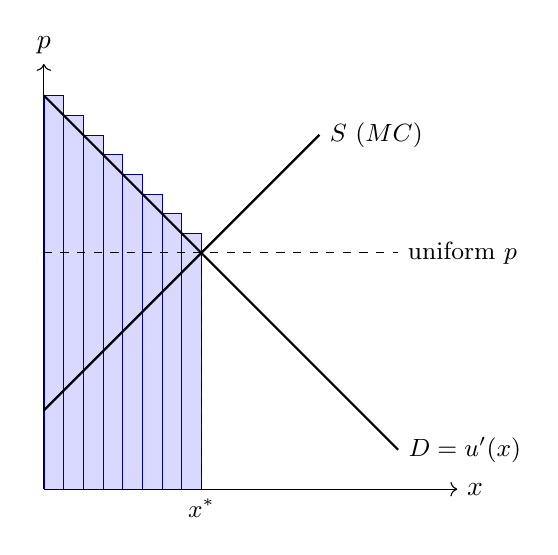
\begin{tikzpicture}[scale=0.5]
\foreach \k in {0,...,7}{
  \pgfmathsetmacro{\xl}{0.5*\k}
  \pgfmathsetmacro{\h}{10-0.5*\k}
  \fill[blue!15] (\xl,0) rectangle ({\xl+0.5},\h);
  \draw[blue!50!black,very thin] (\xl,0) rectangle ({\xl+0.5},\h);
}
\draw[->] (0,0)--(10.5,0) node[right]{$x$};
\draw[->] (0,0)--(0,10.8) node[above]{$p$};
\draw[thick] (0,10)--(9,1) node[right]{\small $D=u'(x)$};
\draw[thick] (0,2)--(7,9) node[right]{\small $S$ ($MC$)};
\draw[dashed] (0,6)--(9,6) node[right]{\small uniform $p$};
\draw[dashed] (4,0) node[below]{\small $x^*$}--(4,6);
\end{tikzpicture}
\end{center}
\textit{How to read the figure.} The shaded strips are the per-unit prices $p_1,p_2,\dots$ under per-unit pricing; each strip's height is the willingness to pay for that piece. Their total area is the area under the demand curve up to $x^*$, $u(x^*)$, which is also the bundle price. Under uniform pricing the consumer pays only the horizontal line $p$ on every unit and keeps the area between demand and that line.

\paragraph{Second-degree price discrimination (nonlinear pricing).} The firm's revenue is a nonlinear function of the amount purchased (e.g.\ quantity discounts). With two consumers, $u_1(x_1)+y_1$ (low demand) and $u_2(x_2)+y_2$ (high demand), the assumption above that the consumer with the larger \emph{total} willingness to pay also has the larger \emph{marginal} willingness to pay ($u_2>u_1$ and $u_2'>u_1'$) is known as the \textbf{single-crossing property}. It is what lets the seller design a menu of (quantity, payment) bundles that the two types choose between voluntarily (self-selection). The full second-degree analysis is not developed in these notes.

%======================================================================
\subsection{Third-degree price discrimination \pg{59--61}}

\paragraph{Setup.}
\begin{itemize}
\item Two identifiable groups (markets) $i=1,2$; the firm can enforce the division (e.g.\ by age for discounts), so there is no resale.
\item $p_i(x_i)$: inverse demand of group $i$; $x_i$ is the quantity sold to group $i$.
\item Constant marginal cost $c$.
\item Elasticity in market $i$: $\epsilon_i=\dfrac{dx_i}{dp_i}\dfrac{p_i}{x_i}<0$, written $|\epsilon_i|$ in absolute value.
\end{itemize}
Within each group every unit sells at one price, but the prices can differ across groups.

\paragraph{Separate markets.} The firm solves
\[
\max_{x_1,x_2}\ p_1(x_1)\,x_1+p_2(x_2)\,x_2-cx_1-cx_2 .
\]
The objective is additively separable, so each market is a separate monopoly problem. FOCs:
\begin{align*}
p_1(x_1)+p_1'(x_1)\,x_1&=c, & p_2(x_2)+p_2'(x_2)\,x_2&=c .
\end{align*}
Rewrite each in elasticity form exactly as in \eqref{eq:micro-markup}:
\begin{equation}\label{eq:micro-3rd}
p_1(x_1)\Big[1-\frac{1}{|\epsilon_1|}\Big]=c,\qquad p_2(x_2)\Big[1-\frac{1}{|\epsilon_2|}\Big]=c .
\end{equation}
Both left-hand sides equal $c$, so $p_1\big[1-1/|\epsilon_1|\big]=p_2\big[1-1/|\epsilon_2|\big]$, i.e.
\[
\frac{p_1}{p_2}=\frac{1-1/|\epsilon_2|}{1-1/|\epsilon_1|}.
\]
The right side exceeds $1$ iff $1-1/|\epsilon_2|>1-1/|\epsilon_1|$ iff $|\epsilon_2|>|\epsilon_1|$.

\begin{keybox}[title=Inverse-elasticity rule]
\[
p_1>p_2\iff|\epsilon_1|<|\epsilon_2| .
\]
The market with the more elastic demand (the more price-sensitive group) is charged the lower price.
\end{keybox}

\paragraph{Linked markets.} Suppose the firm cannot separate the markets cleanly, so the quantity sold in one market affects willingness to pay in the other: $p_i=p_i(x_1,x_2)$. The firm solves
\[
\max_{x_1,x_2}\ p_1(x_1,x_2)\,x_1+p_2(x_1,x_2)\,x_2-cx_1-cx_2 .
\]
Now $x_1$ affects revenue in market 2 as well. FOCs:
\begin{align*}
\frac{\partial}{\partial x_1}:\quad p_1+\frac{\partial p_1}{\partial x_1}\,x_1+\frac{\partial p_2}{\partial x_1}\,x_2&=c,\\
\frac{\partial}{\partial x_2}:\quad p_2+\frac{\partial p_2}{\partial x_2}\,x_2+\frac{\partial p_1}{\partial x_2}\,x_1&=c.
\end{align*}
Defining the own-market elasticity by $\frac{1}{\epsilon_i}=\frac{\partial p_i}{\partial x_i}\frac{x_i}{p_i}$ and factoring $p_i$ out of the first two terms, as before:
\begin{align}
p_1\Big[1-\frac{1}{|\epsilon_1|}\Big]+\frac{\partial p_2}{\partial x_1}\,x_2&=c, \label{eq:micro-link1}\\
p_2\Big[1-\frac{1}{|\epsilon_2|}\Big]+\frac{\partial p_1}{\partial x_2}\,x_1&=c. \label{eq:micro-link2}
\end{align}
\emph{Symmetry of cross effects.} With quasilinear utility $u(x_1,x_2)+y$, the inverse demands are $p_i=\partial u/\partial x_i$, so (Young's theorem: cross-partials are equal)
\[
\frac{\partial p_1}{\partial x_2}=\frac{\partial^2u}{\partial x_2\,\partial x_1}=\frac{\partial^2u}{\partial x_1\,\partial x_2}=\frac{\partial p_2}{\partial x_1}\equiv u_{12}.
\]
Subtract \eqref{eq:micro-link2} from \eqref{eq:micro-link1} and use this symmetry:
\begin{align*}
p_1\Big[1-\tfrac{1}{|\epsilon_1|}\Big]-p_2\Big[1-\tfrac{1}{|\epsilon_2|}\Big]+u_{12}\,x_2-u_{12}\,x_1&=0\\
p_1\Big[1-\tfrac{1}{|\epsilon_1|}\Big]-p_2\Big[1-\tfrac{1}{|\epsilon_2|}\Big]&=(x_1-x_2)\,\frac{\partial p_2}{\partial x_1}.
\end{align*}

\emph{Sign of the cross effect.} The two groups buy the same good, so it is natural to treat the two ``goods'' as \textbf{substitutes}: selling more to group 1 lowers group 2's willingness to pay, $\partial p_2/\partial x_1=u_{12}<0$. (Formally: inverting the inverse demands, $\partial x_1/\partial p_2=-u_{12}/\det H$ where $H$ is the Hessian of $u$, with $\det H>0$ by strict concavity; substitutes, $\partial x_1/\partial p_2>0$, means $u_{12}<0$.)

Now suppose $x_1>x_2$. Then the right-hand side $(x_1-x_2)\,u_{12}<0$, so
\begin{align*}
p_1\Big[1-\tfrac{1}{|\epsilon_1|}\Big]&<p_2\Big[1-\tfrac{1}{|\epsilon_2|}\Big]\\
\frac{p_1}{p_2}&<\frac{1-1/|\epsilon_2|}{1-1/|\epsilon_1|} &&\text{(divide by $p_2[1-1/|\epsilon_1|]>0$).}
\end{align*}
If $|\epsilon_1|>|\epsilon_2|$, then $1-1/|\epsilon_1|>1-1/|\epsilon_2|$, the right side is below $1$, and therefore $p_1<p_2$.

\emph{Interpretation:} as with separate markets, the more elastic market (here market 1, which also buys more) gets the lower price. The cross effect matters for the exact prices, but with substitutes it does not overturn the inverse-elasticity ranking.

\paragraph{Welfare effect: setup.}
\begin{itemize}
\item Two groups summarized by quasilinear utility $u(x_1,x_2)+y$ with $u$ concave, so $p_i(x_1,x_2)=\partial u(x_1,x_2)/\partial x_i$.
\item $c(x_1,x_2)$: cost of providing $x_1$ and $x_2$. Social welfare $W(x_1,x_2)=u(x_1,x_2)-c(x_1,x_2)$.
\item Two situations to compare: an initial one $(x_1^0,x_2^0)$ with prices $(p_1^0,p_2^0)$, and a new one $(x_1',x_2')$ with prices $(p_1',p_2')$. Write $\Delta x_i=x_i'-x_i^0$, $\Delta u=u(x')-u(x^0)$, $\Delta c$, $\Delta W=\Delta u-\Delta c$.
\end{itemize}
\emph{Question:} does moving to third-degree price discrimination raise social welfare?

\paragraph{Bounds on $\Delta u$.} Apply the concavity inequality (a concave function lies below its tangent plane) twice.
\begin{itemize}
\item Tangent plane at $x^0$, evaluated at $x'$:
\begin{align*}
u(x_1',x_2')&\le u(x_1^0,x_2^0)+\frac{\partial u(x^0)}{\partial x_1}(x_1'-x_1^0)+\frac{\partial u(x^0)}{\partial x_2}(x_2'-x_2^0)\\
\Delta u&\le p_1^0\,\Delta x_1+p_2^0\,\Delta x_2 &&\text{(use $p_i^0=\partial u(x^0)/\partial x_i$).}
\end{align*}
\item Tangent plane at $x'$, evaluated at $x^0$:
\begin{align*}
u(x_1^0,x_2^0)&\le u(x_1',x_2')+p_1'\,(x_1^0-x_1')+p_2'\,(x_2^0-x_2')\\
\Delta u&\ge p_1'\,\Delta x_1+p_2'\,\Delta x_2 &&\text{(rearrange; flip signs).}
\end{align*}
\end{itemize}
Subtract $\Delta c$ throughout:
\[
p_1^0\,\Delta x_1+p_2^0\,\Delta x_2-\Delta c\ \ge\ \Delta W\ \ge\ p_1'\,\Delta x_1+p_2'\,\Delta x_2-\Delta c .
\]
With constant marginal cost, $\Delta c=c\,\Delta x_1+c\,\Delta x_2$, so
\begin{equation}\label{eq:micro-wbounds}
(p_1^0-c)\,\Delta x_1+(p_2^0-c)\,\Delta x_2\ \ge\ \Delta W\ \ge\ (p_1'-c)\,\Delta x_1+(p_2'-c)\,\Delta x_2 .
\end{equation}

\paragraph{Applying the bounds to price discrimination.} Let the initial situation be uniform monopoly pricing (no discrimination), $p_1^0=p_2^0=p^0$, and let $(p_1',p_2')$ be the discriminatory prices. Then \eqref{eq:micro-wbounds} becomes
\[
(p^0-c)\,(\Delta x_1+\Delta x_2)\ \ge\ \Delta W\ \ge\ (p_1'-c)\,\Delta x_1+(p_2'-c)\,\Delta x_2 .
\]
\begin{itemize}
\item \textbf{Upper bound.} A monopolist prices above marginal cost, $p^0-c>0$. If total output fell, $\Delta x_1+\Delta x_2<0$, the upper bound would be negative and so $\Delta W<0$. Hence welfare can rise only if total output rises.
\item \textbf{Lower bound.} If the price-cost-weighted sum of output changes is positive, then $\Delta W$ is above a positive number, so welfare rises.
\end{itemize}
\begin{keybox}[title=Welfare effect of third-degree price discrimination]
\begin{itemize}
\item \textbf{Necessary} for $\Delta W>0$: total output increases, $\Delta x_1+\Delta x_2>0$.
\item \textbf{Sufficient} for $\Delta W>0$: $\sum_i(p_i'-c)\,\Delta x_i>0$.
\end{itemize}
\end{keybox}
\emph{Interpretation:} discrimination moves units from one group to the other. At the uniform price every unit has the same marginal value $p^0$, so merely reshuffling a fixed total cannot help; welfare can rise only if discrimination expands total sales (e.g.\ by opening a market that the uniform price left unserved).

\paragraph{Example: linear demands, zero marginal cost.} Let $x_i=a_i-b_ip_i$ ($a_i,b_i>0$), so $p_i(x_i)=(a_i-x_i)/b_i$, and let $c=0$.

\emph{With discrimination,} the firm maximizes revenue in each market separately:
\begin{align*}
&\max_{x_i}\ R_i(x_i)=\frac{a_i-x_i}{b_i}\,x_i=\frac{a_ix_i-x_i^2}{b_i}\\
&\frac{dR_i}{dx_i}=\frac{a_i-2x_i}{b_i}=0 &&\text{(FOC, $MR=MC=0$)}\\
&x_i=\frac{a_i}{2},\qquad x_1+x_2=\frac{a_1+a_2}{2}.
\end{align*}
\emph{Without discrimination,} the firm chooses one price $p$ for both markets:
\begin{align*}
&R(p)=p\,(x_1+x_2)=p\big[(a_1-b_1p)+(a_2-b_2p)\big]=(a_1+a_2)\,p-(b_1+b_2)\,p^2\\
&R'(p)=(a_1+a_2)-2(b_1+b_2)\,p=0 &&\text{(FOC)}\\
&p^*=\frac{a_1+a_2}{2(b_1+b_2)} &&\text{(solve for $p$)}\\
&x_1+x_2=(a_1+a_2)-(b_1+b_2)\,p^*=(a_1+a_2)-\frac{a_1+a_2}{2}=\frac{a_1+a_2}{2}. &&\text{(substitute)}
\end{align*}
Total output is the same under both regimes, $\Delta x_1+\Delta x_2=0$. By the upper bound, $\Delta W\le(p^0-c)\cdot 0=0$.

\begin{keybox}[title=Linear demand result]
With linear demands and both markets served at the uniform price (i.e.\ $a_i-b_ip^*\ge 0$ for $i=1,2$), third-degree price discrimination leaves total output unchanged and therefore cannot raise welfare: $\Delta W\le 0$ (typically $<0$, because output is misallocated across the groups).
\end{keybox}

\end{document}
